\documentclass[11pt]{book}
\usepackage{hyperref,fancyhdr,setspace,graphicx,eurosym}
\usepackage[utf8]{inputenc}
\usepackage[spanish,activeacute]{babel}

\pagestyle{fancy}
\renewcommand{\chaptermark}[1]{\markboth{\emph{\thechapter.\ #1}}{}}
\renewcommand{\sectionmark}[1]{\markright{\emph{\thesection.\ #1}}{}}
\renewcommand{\footrulewidth}{1px}
\fancyhf{}
\fancyhead[LE,RO]{\thepage}
\fancyhead[CO]{\rightmark}
\fancyhead[CE]{\leftmark}
\fancyfoot[C]{\thepage}

\addto\captionsspanish{
  \def\contentsname{\'Indice}
}

\begin{document}

\frontmatter
\title{Relatos de distintos viajes}
\author{Eugenio Costa}
\date{}
\maketitle
\thispagestyle{empty}

\cleardoublepage

\thispagestyle{empty}
\begin{flushright}
\item \emph{\small A mis viejos. \textexclamdown Gracias!}
\item \emph{\small A Ezequiel, Eugenio y Guido.\\
Buenos amigos son columna de un buen viaje.}
\end{flushright}

\clearpage
\thispagestyle{empty}
\tableofcontents
\thispagestyle{empty}

\clearpage
\thispagestyle{empty}
\setcounter{page}{1}
\chapter{Introducci\'on}

\begin{flushright}
\item \emph{\small ``Lo mejor de los viajes es lo de antes y lo de despu\'es.''\\
Maurice Maeterlinck}
\end{flushright}

\section{La bici}

Desde que nac\'i en 1985 hasta algunos a\~nos despu\'es pedale\'e muy poco.
\textexclamdown Es que heredaba una bici con rueditas estabilizadoras de
pl\'astico duro, que hac\'ian tanto ruido que me daba verg\"uenza usarla! Por
eso demor\'e en aprender a pedalear sin rueditas. Y pensar que ahora me
vendr\'ia muy bien instalar un par.

Tiempo despu\'es, a la hora de la siesta pap\'a me llevaba a la calle con la
misma bicicleta pero ya sin las rueditas. Me dec\'ia que no mire atr\'as y me
empujaba hasta mantener un equilibrio, para soltarme silenciosamente.
\textexclamdown Era incre\'ible poder andar tan r\'apido y sin ruidos! Pero
siempre terminaba mirando atr\'as sabiendo que no me acompa\~nar\'ia, y el
intento de aprendizaje terminaba en porrazo y pocos raspones. \textexclamdown Si
a golpes se hacen los hombres, gozo de virilidad desde peque\~no!

A mis diez a\~nos me regalaron una bici rojita con buenos frenos, con la que
empec\'e a andar. Pero esos d\'ias lo hac\'ia porque se supon\'ia que lo
hiciera, como cualquier otro juego, y no porque de verdad lo eligiera.

Empec\'e a admirar luego una hermosa bicicleta, me encantaba. Estaba en una
bicicleter\'ia nueva, y yo iba siempre a molestar al vendedor con preguntas y
a mirarla. No pod\'ia creer que trajera un nuevo sistema de cambios y que se
viera tan bien. Hasta el nombre me gustaba, la relativamente simple
``Talera'', que para un chico de once a\~nos era una locura. Desde que mis
viejos me la regalaron pedaleo porque de verdad me gusta, fue mi deporte
elegido. En casa ten\'iamos que practicar por lo menos un deporte, y \'este
era el que m\'as me divert\'ia.

Andaba sin parar, el vendedor me alentaba a andar siempre r\'apido para
entrenar. No pod\'ia ir de casa al centro paseando, lo ten\'ia que hacer
exigido. Cada vez pod\'ia un poquito m\'as, aunque todav\'ia era chico.

Dos amigos tambi\'en se compraron buenas bicis, y los dem\'as usaban la de
siempre: ``la rojita'', ``la freestyle'' o ``la cl\'asica'' eran algunas.
Pase\'abamos mucho, organiz\'abamos carreras en las plazas, practic\'abamos
piruetas, tambi\'en jug\'abamos a la mancha, que era lo m\'as cansador y
divertido. Termin\'abamos exhaustos o siendo ``mancha''.

Planeaba correr carreras pero consegu\'i competir en cuatro, perdiendo as\'i
el campeonato. La m\'as larga fue bajo lluvia y sobre barro. Hab\'ia ido poca
gente porque a nadie se le ocurri\'o viajar con lluvia, \textexclamdown con
decir que en mi categor\'ia corr\'iamos dos! Y llegu\'e al glorioso segundo
puesto. Tambi\'en el trofeo la hace inolvidable.

Pas\'o un tiempo. Para entrenar no nos bastaba con andar r\'apido por la ciudad
hasta llegar a las plazas. Nos dedicamos a tomar caminos de tierra, atravesando
campos y llegando a pueblos. Los lugares \'infimos y ``perdidos'' empezaron a
ser usuales. Nos alej\'abamos para conocer, todo nos sorprend\'ia.
(\textexclamdown Esto no cambi\'o mucho!) Una tarde de sol salimos todos los
amigos hacia ``la olla'', un lugar a 25~km de Pergamino que nos hab\'ian
recomendado conocer. \textexclamdown El primer viajecito! Uno desert\'o a 5~km
de la salida, el pobre ven\'ia cargando toda el agua del grupo. Otros se
demoraban, pero casi todos cubrimos los 50~km planeados. Al llegar a casa tan
transpirado no par\'e de hablar de lo nuevo que hab\'iamos conocido.
\textexclamdown Tan hermoso y tan cerquita!

No todos siguieron yendo. De hecho, s\'olo a dos nos encant\'o y no dejamos de
ir. Mi amigo y compa\~nero de viajes Ezequiel, y yo. Para los chicos era una
actividad m\'as aparte de tantas otras, un d\'ia de encuentros. Eventualmente
nos acompa\~naban. Para nosotros en cambio era nuestro modo de divertirnos y
deporte elegido.\\

Lleg\'o en esos momentos el primer viaje diferente: a mis 14 a\~nos, un amigo
de mi viejo me invit\'o a hacer el cruce de la Cordillera en bici por Mendoza.
Viaj\'abamos Julio Godoy --quien organizaba--, Gustavo Bozicovich --un amigo--,
mi t\'io Carlitos al volante, y yo. As\'i conoc\'i los caracoles chilenos, y
los baj\'e en dos ruedas. Adelant\'e al primer cami\'on de mi vida, era de
ciencia ficci\'on. Las im\'agenes, sonidos y olores de ese viaje nunca dejaron
de rodar por mi cabeza. Estaba admirado por conocer cosas nuevas y diferentes,
hermosas. Casi no conoc\'ia las monta\~nas.

Despu\'es de ese recorrido volv\'i a la divertida rutina de la escuela, y en
las tardes a ``la olla'' con Ezequiel. Durante las varias horas de pedaleo no
par\'abamos de charlar ni de re\'ir. El camino se nos empez\'o a tornar
mon\'otono y tomamos entonces otros. Empezamos a conocer en cada salida un
pueblo nuevo, llegamos a conocer casi todos en el radio de 30~km desde nuestra
ciudad. Gelo Godoy, con sus 90 a\~nos, nos mostr\'o varios caminos para
recorrer a pedal.

Todo esto nos llev\'o a querer viajar en bici. Cuando coment\'e en casa la idea
que plane\'abamos para un verano --unir los 7 lagos, desde San Mart\'in de los
Andes hasta Bariloche-- no me dejaron hacerlo. No creyeron prudente dejarme
emprender un viaje de aventuras a mis 17 a\~nos. Ir a Mar del Plata en familia y
con bici, despu\'es de todo, en absoluto me disgustaba. Todav\'ia no a\~noraba
lo que no conoc\'ia.

En esas vacaciones no dej\'e de pedalear, la pasi\'on segu\'ia mudada al mar y
sin alforjas. La playa quedaba a 16~km de casa, el camino era una delicia.
Conoc\'i adem\'as todos los rincones de la gran ciudad.

De vuelta en Pergamino pedaleamos Ezequiel y yo a Pe\~na, pueblo peque\~nito e
hist\'orico. Paramos en un antig\"uo parador a tomar algo y seguimos, curiosos,
alimentando esas ganas de viajar en bici. Este fue mi \'ultimo viaje en la
hermosa y ya desgastada bici, pues la robaron. Sabiendo que no ven\'ia mal el
cambio, los viejos me consiguieron una bicicleta excelente para seguir andando.

Llegu\'e a entenderme con el nuevo veh\'iculo casi al momento de subirme: lo
sent\'ia como una moto. Los cambios eran r\'apidos y precisos, \textexclamdown
y los frenos tan potentes!

Ir a la escuela en eso era un verdadero placer, no me importaban los calores del
verano ni los fr\'ios del invierno. Usaba pocos minutos en cubrir esos casi
cuatro kil\'ometros, lo controlaba siempre. No dejaba un momento sin hacer
fuerza. Recuerdo que una ma\~nana cruc\'e un auto a tres cuadras de casa, y nos
volvimos a cruzar al llegar: hab\'ia llegado tan r\'apido como el veh\'iculo
motorizado. \textexclamdown Qu\'e hermosa euforia, despu\'es de la exigencia
f\'isica!

Llegaba transpirad\'isimo sin excepci\'on, mis amigos me cargaban. La dejaba
en sus casas, esperaba a que desayunaran sin buzo ni remera para no
transpirarlos, y me miraban como a un loco. A la salida de la escuela
tambi\'en pedaleaba tanto como pod\'ia. Presum\'ia adelantando a las otras
bicis por la derecha, \textexclamdown y si pod\'ia por el medio de dos, mucho
mejor! Qu\'e peligroso era, y qu\'e hermoso fue. No me alegra, pero es eso lo
que a veces disfruto.

Un d\'ia llegaba tarde a clase, y por atar la ``ametralladora'' a un poste
fuera de la escuela tambi\'en me la robaron. Esta vez el mal trago fue
dif\'icil de digerir porque esa bici era la continuaci\'on de mi cuerpo. Pero
los viejos lograron conseguirme la tercera y actual bici, tan buena y
confiable como la ``Talera'', pero no fuera de serie como \'esta. Una
bicicleta para andar kil\'ometros sin preocuparme por su estado, tal como
necesito. \textexclamdown Ya lleva cuatro viajes ``largos'' el fiel
transporte! E incontables cortos.

\section{Los viajes}

Finalizado el secundario y cumplidos los 18, ten\'ia permitido salir de viaje
con amigos. Entonces empezamos. El primer viaje ``planeado'' por nosotros (el
plan fue comprar un pasaje a Jun\'in de los Andes, un primo nos organiz\'o el
itinerario d\'ias antes de la salida) fue excelente. Tomamos dos semanas para
completar 450~km, viaj\'abamos muy despacio por el peso de las alforjas y para
conocer de modo placentero un paisaje tan distinto a nuestras pampas. Volvimos
felices, hab\'iamos conocido algo totalmente nuevo, un diferente estilo de
vida m\'as simple, m\'as escencial. En el reencuentro de amigos est\'abamos
seguros de que esta era la mejor opci\'on a la hora de salir de vacaciones, y
los otros ocho tambi\'en sent\'ian lo mismo al relatarnos lo que se
divirtieron juntos por la costa. La eterna decisi\'on: mochila y monta\~nas, o
casa y playas.

Pas\'o un a\~no de estudios con poco ejercicio f\'isico, un Diciembre de
pedaleos ininterrumpidos, y llegaron las fiestas del fin del a\~no 2004.
Ezequiel y yo tomamos un colectivo apenas comenzado el 2005 a San Rafael,
Mendoza: plane\'abamos el cruce de la Cordillera, por la {\small RN}7 hasta el
Oc\'eano Pac\'ifico (Vi\~na del Mar, en Chile). Otro viaje ``redondo'' en que
cubrimos el doble de kilometraje que en el primero, 900~km.

D\'ias despu\'es del fascinante cruce llegu\'e a Mar del Plata, donde me
esperaba la familia veraneante. Rearm\'e la bici en la terminal con la ayuda
de un turista, y llegu\'e a la casa pedaleando. Me acuerdo de sus expresiones,
\textexclamdown nunca me hab\'ian visto con barba! Entre fotos y relatos no
par\'e de hablar, empapado de emoci\'on mientras iba entendiendo todo lo que
hab\'iamos hecho. Se sorprend\'ian porque durante dos d\'ias com\'i sin
descanso: desaparec\'ia la panera llena de tostadas, todas las milanesas de la
fuente, despu\'es (y mientras todos com\'ian postres, ya cansados de esperarme)
terminaba con la ensalada que sobraba. \textexclamdown La vieja se preocupaba!
Me ba\~naba dos veces al d\'ia. Dorm\'ia c\'omodamente, mucho. Se vuelve al
hogar y se vive lo mismo que antes de la salida, pero vi\'endolo desde otro
punto de vista, otro modo de pensarlo. Es apasionante vivir estas dos vidas en
el mismo a\~no.

Ese Enero llegu\'e a Pergamino con mil ideas por contarles a mis viejos: todos
los proyectos que hab\'iamos tratado durante el viaje con mi amigo. En una cena
les coment\'e, luego de toda una lista de viajes por Am\'erica, que a modo de
broche de oro, al recibirnos de Ingenieros, nos gustar\'ia dar una buena vuelta
por Europa, antes de empezar la vida de ``adultos'' con trabajo fijo. (Luego me
cambi\'e a Ciencias de la Computaci\'on, \textexclamdown menos mal que pap\'a no
acept\'o!) \textexclamdown Para so\~nar lo hacemos en grande! Es que el mundo es
enorme e interesante. Pap\'a contest\'o, con una simpleza imposible:
``\textquestiondown Porqu\'e no te vas ahora? No sab\'es si al recibirte lo vas
a poder hacer''. Abr\'i la boca, pero qued\'e mudo. Y sigui\'o: ``Comunicate con
nuestros amigos, seguro te van a ayudar''.

Un cuatrimestre de estudios, el vuelo transatl\'antico, un viaje
\emph{distinto}, muchos escritos, y la vuelta.

Ya en Diciembre, festejamos el A\~no Nuevo de 2006 en casa, y esa misma
madrugada salimos Ezequiel y yo a pedalear por Argentina. Quer\'iamos llegar
para ese Febrero a Ushuaia partiendo desde Bariloche, alrededor de 2.000~km de
Patagonia; pero diversos contratiempos nos llevaron a conformarnos con unir San
Mart\'in de los Andes con Esquel, alrededor de 800~km. \textexclamdown Conoc\'i
los l\'imites, que hasta entonces nunca se me hab\'ian presentado! Sin embargo
logr\'e disfrutar mucho de este paseo, porque luego de un viaje en bici solo por
Alemania, dependiendo de internet para sentirme acompa\~nado, ya no me importaba
estar en Villa la Angostura en vez de m\'as cerca de Ushuaia; con un amigo todo
era diferente. No necesitaba hacer cosas enormes para divertirme, basta con
estar bien acompa\~nado y con buena voluntad.

Despu\'es conocimos el Noroeste Argentino, y luego Bolivia y Per\'u (aunque esta vez de mochileros); nuevos viajes perfectos, cada cual con su particularidad.

\section{Los diarios, y el libro}

Al embarcarnos Eze y yo en nuestro primer viaje en bici, mis viejos, un tanto
preocupados, me pidieron que enviara noticias siempre que pudiera. Al
encontrar cyber-caf\'es me sentaba a escribir unas l\'ineas informativas, pero
no pod\'ia parar de escribir. La cantidad de cosas que conocimos fue
apabullante, y compartirlo es para mi otro modo de seguir disfrutando.
\textquestiondown Qu\'e placer m\'as grande que volver a casa y contar un
viaje? \textexclamdown Yo empezaba a hacerlo desde la misma ruta, gracias a la
red! Me respond\'ian a estos mensajes que escribiera m\'as, para mantenerlos
al tanto y para tener el recuerdo siempre fresco. Entonces, durante el viaje
por Mendoza, escrib\'i m\'as. Y de nuevo la misma cadena de elogios y
recuerdos guardados. Releer esos escritos durante el a\~no es para m\'i volver
a sentirlos.

Al viajar a Europa supuse que escribir\'ia bastante, \textexclamdown pero no
imaginaba tanto! Mis amigos bromeaban diciendo que no les alcanzaba el tiempo
para leerlos, la familia se alegraba y quer\'ia a\'un m\'as detalles. As\'i es
que no dej\'e pasar tres d\'ias, siempre ten\'ia una computadora conectada a
mano, y siempre ocupaba una hora de inactividad tur\'istica para escribirles.
Entonces quise escribir. \textexclamdown Era tal placer hacerlo sabiendo que
en Argentina familiares, amigos y hasta conocidos no tan cercanos esperaban
con ganas esos diarios! Y no escrib\'ia pensando en revivirlo dentro de tres
meses, ni en los elogios y buenos deseos que me llenaban de entusiasmo; lo
hac\'ia revivi\'endolo en ese preciso instante, al intentar llevar lo
descripto a quienes leyeran. Revisaba las fotos del d\'ia para no olvidar
ning\'un momento, realmente lo volv\'ia a vivir.

As\'i junt\'e esa cantidad de escritos que insin\'uan un libro. Y le di forma,
con la esperanza de alg\'un d\'ia imprimirlo y poder compartir esas vivencias
m\'as all\'a de mi familia. Significar\'a mi mayor satisfacci\'on que ustedes,
al leer estos relatos, los puedan vivir tambi\'en conmigo.\\

\textbf{Nota preliminar:}

Notar\'an que cada viaje tiene un estilo de escritura distinto, quise
mantenerlos tanto como el libro permitiera. Espero haber logrado un equilibrio
entre la correcci\'on y cierta imparcialidad que merece un texto descriptivo, y
la c\'alida frescura de los relatos originales.

\mainmatter

\chapter{Los 7 Lagos, de Jun\'in de los Andes a Bariloche}
\begin{flushright}
\item \emph{\small ``No escuches lo que dicen. And\'a, miralo.''\\
Proverbio chino}.
\end{flushright}
\section{Primeros d\'ias, lago Huechulaufquen}

Estoy en San Mart\'in de los Andes, y les cuento que estoy de diez. Esto es
incre\'ible, no lo puedo creer. El primer d\'ia embarcamos en las bicis hacia el
lago Huechulaufquen. \textexclamdown Eran las 2am y segu\'iamos pedaleando,
desde las 6:30pm! Nos agarr\'o la noche como a los mejores, pero seguimos a pie,
a la luz de la luna llena, que iluminaba la enormidad del lago. A las tres de la
ma\~nana paramos en el primer campamento que se nos cruz\'o, y empezamos a armar
la carpa y el calentador para cenar unos ricos capeletinis de verdura. Comimos,
ordenamos, y a la bolsa. A las 10:30 nos levantamos, fuimos al lago a lavar las
cosas, ordenamos todo, y partimos hacia el lago Paim\'un, muertos despu\'es de
las cinco horas de caminata/pedaleo de ayer con peso y monta\~na.
\textexclamdown Adem\'as, este primer d\'ia nos toc\'o viento en contra!

Hacia el Paim\'un tuvimos unas bajadas fenomenales. Con todo el peso de las
alforjas sobre la rueda de atr\'as, la delantera bailaba. A 25~km/h parec\'ian
240~km/h; y no nos lastimamos, lo que no quita que no nos hayamos ca\'ido.
Llegu\'e a 47~km/h y Ezequiel iba m\'as r\'apido. Un entretenido peligro en esas
bajadas-subidas, curvas-contracurvas, etc-etc.

Perdidos pas\'abamos el Paim\'un, cuando nos encontramos con Alfon --mi primo--
de pura casualidad. \textexclamdown Llegaban justo de cortar le\~na! Volvimos a
su campamento, donde nos esperaban los cuatro amigos con una trucha (que no fue
pescada por ellos, \textexclamdown aunque intentaron!) y algunos choclitos
hervidos. Luego caminamos a una cascada, que pudimos ver desde abajo y desde
atr\'as. \textexclamdown Parec\'ia una catarata y ten\'ia s\'olo 5 metros! De
los 45 minutos que tomaba llegar, 15' eran trepando una mota\~na a trav\'es de
rocas. Inolvidable.

Volvimos a ver c\'omo pescaban con mosca, un embole, pero al lado del lago y a
los pies de los cerros y del volc\'an Lan\'in, no la pasamos muy mal que
digamos. Dormimos ah\'i, y salimos la siguiente ma\~nana en un cole a San
Mart\'in de los Andes.

Aqu\'i estoy, despu\'es de dar unas vueltas para reconocer terreno. Fuimos a una
farmacia para ver qu\'e le pasa a Eze, y aunque le digan que no pasa nada no se
puede ni mover. No s\'e si sigue, vuelve o se queda, pero ma\~nana me gustar\'ia
seguir, lo vemos esta noche.

Un fuerte abrazo a todos, estoy de diez ac\'a en el Sur, conociendo. Bueno, nada
m\'as, muchas gracias, viejos;

Tute.

\section{Por la ruta de los 7 Lagos}

Eze se sinti\'o mejor, as\'i que de San Mart\'in de los Andes salimos hacia el
Lago Hermoso. Fue un poco duro pero estuvo mortal. Pasamos por el lago L\'acar
(donde compr\'e el pasaje, llego a Mar del Plata el 21 a la noche,
\textexclamdown espero carne con tomates!), el Mach\'onico (se ve\'ia lindo;
ah\'i habl\'e con un propietario de un {\small VW} Passat, \textexclamdown un
mentiroso sobre su auto!); y llegamos al lago Hermoso, donde acampamos y la
pasamos fr\'io. Venimos corriendo carreras porque ya estamos en Villa la
Angostura y pasado ma\~nana en ``Baril\'o'', planeado para dentro de una semana.

Del Hermoso salimos al Espejo Chico, pasando por el Falkner (de los m\'as
lindos), Villarino, y otros que ya no recuerdo. \textexclamdown Cierto, el
Escondido! Divino. Ten\'iamos tres capas de transpiraci\'on con sus respectivas
tres capas de tierra pegadas. Asquerosamente divertido.

Dormimos en el Espejo Chico, hermos\'isimo lago. Al fondo se empiezan a ver los
picos nevados de la Cordillera, m\'as cerca de la costa se ven truchas saltando,
y hay flores amarillas por todo el pasto. Un espect\'aculo. Comimos capeletinis
con ``pur\'e Cica'' arriba, riqu\'isimo.

De all\'i nos fugamos para Villa la Angostura. Pasamos por otros lagos, nos
cansamos mucho; por ese ripio con piedras a 25~km/h se sent\'ia como a 80~km/h.
Pero la cosa es que no \'ibamos a 25, \textexclamdown llegamos a 45~km/h con
alforjas y todo! Arribamos sanos y salvos y vivos, una bajada inolvidable. De
verdad. Cubiertos por un t\'unel de \'arboles y \'arboles que nos hac\'ian
sombra, en bicis sobre el ripio\ldots\ es un sue\~no que se hace realidad.
Pasamos por Pichi Traful, un camping muy organizado pero m\'as lleno que Punta
Mogotes en Mar del Plata, as\'i que seguimos a la Villa. Fue un poco cansador.

Mucha gente en el camino nos tira buena onda, algunos no lo pueden creer. Nos
cruzamos un paral\'itico en una especie de triciclo movido por sus brazos.
\textexclamdown Con una camioneta de apoyo recorr\'ia los 7 lagos! Hay que tener
fuerza de voluntad para hacer eso. Y ganas de vivir. Un grande.

\textexclamdown Olvidaba de contar sobre una subida largu\'isima y terrible con
viento en contra! Pero eso no es nada, imag\'inennos transpirad\'isimos, con
cada auto ech\'andonos mucha tierra. Pero les digo que no es nada, ahora
imag\'inennos subiendo a 4 km/h en el cambio 1-1, rodeados por \emph{siete}
t\'abanos que se met\'ian en los ojos, orejas, nariz, boca, picaban las piernas,
y qu\'e se yo que m\'as. \textexclamdown El mal humor de Ezequiel fue lo m\'as
divertido que viv\'i, en ese tramo! Fue realmente insoportable pero yo me
divert\'i mucho con esos molestos zumbidos. En la bajada los perdimos, y pudimos
seguir viaje en paz.

En Villa la Angostura conocimos el Parque Nacional Los Arrayanes. A eso no lo
puedo describir ni en video, ni en foto, ni en persona, ni menos que menos
escribiendo. Pero probemos. Eran 12~km a trav\'es de Alerces, Coihues y otras
yerbas, de un camino lleno de subidas y bajadas sin viento, dentro de un t\'unel
de vegetaci\'on del ancho promedio de dos personas y rodeados por el lago Nahuel
Huapi. Ah\'i fuimos r\'apido de verdad, por lo que era el camino. Como las
alforjas estaban en el campamento no hab\'ia problemas en las curvas. Esos 12~km
se nos tornaron 3~km, primera vez de todo el viaje en que lo que hicimos
pareci\'o menos. Recorrimos el parque, incre\'ibles los lisos, fr\'ios y
anaranjados Arrayanes, y volvimos.

Esto merece m\'as que mil palabras; imaginen, simplemente, el para\'iso terrenal
para el cicloturista. Despu\'es de esto no espero nada del Bah\'ia Manzano
recomendado, porque no puedo imaginar algo mejor. El camino a veces estaba
escalonado, o lleno de ra\'ices, as\'i que destrozamos las llantas, pero
de verdad que no tiene precio recorrerlo. Ah\'i s\'i que planeo volver diez
veces por a\~no, m\'as all\'a de los 7 Lagos.

Ya de noche, empezamos a pedalear en busca de alg\'un campamento saliendo de la
Villa. Ezequiel insist\'ia en seguir a la luz de la luna hasta Bariloche, pero
entre cansado e inseguro en la ruta, lo convenc\'i de parar. Encontramos un
campamento pasando Bah\'ia Manzano. Ma\~nana recorreremos por aqu\'i
descansando, ya que pasado viajamos 70~km hasta Bariloche, y lo haremos en un
solo d\'ia. All\'a saldremos de joda una noche, recorreremos el Circuito Chico y
dem\'as yerbas barilochenses. Eso es todo, creo. No\ldots\ qu\'e va a ser todo.
\textexclamdown Qu\'e lindo recordar!

Apenas vimos el Nahuel Huapi desde la ruta nos volvimos locos de la emoci\'on,
pero tambi\'en de la sed y garganta seca. No s\'e estimar pero a m\'as de quince
metros de altura sobre el lago est\'abamos seguro. Empezamos a deslizar tipo
``culi-pat\'in'' por la tierra, ensuciamos todo, pero llegamos a las rocas
cercanas al lago. Fue adrenal\'inico pero vali\'o la pena: ahora pod\'iamos
tomar agua fresca y ve\'iamos pececitos chiquitos recorriendo el lago. La
cuesti\'on era ahora subir, y, obvio, por esa tierra resbaladiza no lo
lograr\'iamos. As\'i que rodeamos un poco el lago, subimos a trav\'es de rocas
un poco flojas, y encontramos plantas. Miramos arriba y ahora era acantilado,
pero siguiendo un poquito m\'as pudimos subir a trav\'es de tierra,
agarr\'andonos de las plantas. Llegamos arriba despu\'es de mucho trepar.
\textexclamdown Casi terminamos el agua que bajamos a buscar en ese viaje cuesta
arriba!

Madre, no sab\'es lo que valieron tus alfajores ``Capit\'an del Espacio'' ac\'a,
en el Sur. Otro comentario sin relaci\'on: de vez en cuando cruzamos un cami\'on
internacional y me dan ganas de manejarlo.

Agarren un mapa porque sino no entender\'an ni la mitad de lo que habl\'e.
\textexclamdown Con decirles que yo aprend\'i bien el mapa recorri\'endolo!

Bueno, si quer\'ian que escribiera, \textexclamdown lo lograron!

Un fuerte abrazo a todos,

Tute.

\section{De Villa la Angostura a\ldots\ \textexclamdown Bariloche!}

Hoy salimos del camping de Bah\'ia Manzano en Villa la Angostura, a recorrer la
bah\'ia. Me hizo acordar mucho a Caril\'o, con la diferencia de que si
gir\'abamos la cabeza a alg\'un lado siempre se ve\'ia el lago. Salimos para
Bariloche sin saber si lleg\'abamos al anochecer o a la madrugada siguiente,
pero el viento quiso que lleg\'aramos a las 8 pm, bien de d\'ia ac\'a en el Sur.
Un viento a favor infartante, las subidas eran planicies, las planicies bajadas,
y las bajadas eran euforia.

Mucha gente saluda a los ciclistas para levantar los \'animos, y lo logran.
Hicimos en un d\'ia 70~km casi, llegamos bien. Nos sacamos fotos en los
\'ultimos carteles de distancias, y calculamos unos 330~km recorridos hasta
ahora, sin contar las vueltas que se avecinan por Bariloche.

Aunque no lo crean\ldots\ \textexclamdown paramos en el mism\'isimo hotel de
nuestro viaje de 5$^\circ$! Nuestra habitaci\'on est\'a justo en frente de donde
dorm\'ia la mitad de nuestro grupo de amigos. \textexclamdown Lindos recuerdos
que hay al volver ah\'i! Pagamos m\'as que siempre, pero se justifica f\'acil:
camas, \textexclamdown s\'abanas!, ducha, inodoro, \textexclamdown bidet!, TV,
alfombra y\ldots\ \textexclamdown jab\'on! \textexclamdown Jab\'on, despu\'es de
ocho d\'ias! Fue incre\'ible. Diez minutos de agua caliente sin que te joda si
alguien abre la canilla fr\'ia y te queme, o la caliente y te congele. Me
enjabon\'e hasta las patillas, y antes de enjuagarme me frot\'e; sobre la
ba\~nera blanca se iba tierra, y tierra, y tierra\ldots\ \textexclamdown
Incre\'ible la cantidad que tra\'ia! \textexclamdown Un asco!

Ma\~nana voy al lavadero, porque la (casi \'unica) remera no solo tiene olor a
humo, transpiraciones o al lago; el jab\'on blanco tambi\'en hace lo suyo. Y
tiene un color marr\'on que mata. Las medias la van a pasar bien en la
lavander\'ia, tambi\'en.

Ahora estamos en un cyber despu\'es de comer una pizzita; ma\~nana nos iremos
del hotel a un campamento libre para no secarnos de plata, y esa ser\'a la noche
de jodas en Bariloche porque lo vamos a encontrar a Eugenio, otro amigo que anda
por ac\'a.

\textexclamdown Hoy por fin voy a dormir sin pasar fr\'io en alg\'un momento de
la noche! Ma\~nana recorreremos algunas calles de Bariloche y el circuito chico.

Ma, llego a ``Mardel'' el 22 a la noche. Nos vemos;

\textexclamdown Tute!

\section{\textexclamdown Lo hicimos! \textquestiondown Y ahora?}

Hicimos el circuito chico, fue entretenido. Vimos de diversos puntos el lago, y
nos cruzamos en el camino --por primera vez de tres-- una Porsche Cayenne Turbo.

Ibamos a 40~km/h en una bajada, cuando me di cuenta de que en ese punto nos
hab\'ian sacado la foto en el viaje de 5$^\circ$ a\~no, con el hotel ``Llao
Llao'' de fondo. Clav\'e los frenos y posamos para otra foto. Subimos hasta la
puerta del hotel, volvimos a bajar, recorrimos la playita frente al lago, y
seguimos. Encontramos un lugarcito entre \'arboles para parar que ten\'ia un
cartel que invitaba a una caminata de 45' hasta el lago Escondido (el de
Bariloche). Dejamos las bicis a la vera del camino (locura) y empezamos.

Nos sacamos una foto con Arrayanes en un peque\~no bosque que encontramos (nos
quitamos las ganas: \textexclamdown no ten\'iamos esa foto del Bosque!) y
caminamos por un camino rodeado de ca\~nas que hac\'ian de t\'unel. Lindo
sendero, con el Nahuel Huapi a veces borde\'andonos. Caminando y corriendo
llegamos de nuevo hasta la ruta del Circuito Chico, \textexclamdown qu\'e
locura! El Circuito Chico es una gran curva, y lo que hab\'iamos hecho con la
caminata era cortar camino por una recta. O sea que hubi\'esemos llegado
tranquilamente al Lago Escondido de haber seguido pedaleando, como luego
har\'iamos. Claro que igual vali\'o la pena: esa caminata fue divina. Volvimos a
donde estaban las bicis, y seguimos.

Despu\'es de una curva y contracurva por la ruta que agarramos muy r\'apido,
llegamos al Escondido, un peque\~no y pintoresco lago usado por nadadores. Un
lindo muelle, y mucha gente. Seguimos el circuito y pasamos por una cascada,
donde paramos a tomar un chocolate y a sacarnos una foto: era un lugar que
tambi\'en visitamos en 5$^\circ$. Continuamos camino, hasta darnos cuenta que
lleg\'abamos al cementerio del monta\~n\'es. Entramos. Lindo lugar: 5' de
caminata cuesta arriba para llegar al pie de una monta\~na, desde donde se
ve\'ia el Lago y varias cruces, historias y cosas. Muy interesante. Seguimos,
paramos en Colonia Suiza donde Eze compr\'o un licor para regalo (con Euge no
nos encontramos de noche, hablando del tema), miramos el paisaje, y continuamos
cuesta abajo entre curvas. A 40~km/h pasamos una curva de 90$^\circ$ que termina
en puente. \textexclamdown Todo era as\'i! Qu\'e lindo. Hab\'ia que frenar
(\textexclamdown en bici!) para no pasarnos en las curvas. Me parece imposible:
en la bici, aparte de poder doblar mucho, nunca se anda tan r\'apido. Ah\'i
s\'i.

Luego de una bajada hab\'ia una curva de 180$^\circ$. Se me empez\'o a cerrar
m\'as de lo que pod\'ia doblar, y tuve que frenar para no caer a la banquina.
Segu\'i hasta que encontr\'e un parador donde esperar a Eze. Com\'i una rica
mitad de cereza que hab\'ia tirada en el camino (la otra mitad estaba podrida,
seguro alguien la tir\'o por la ventanilla), y segu\'i esperando.
\textexclamdown Cuando lleg\'o me cont\'o que en esa cerrada curva casi choca
contra un auto! El auto segu\'ia derecho para tomar un desv\'io, y \'el lo
esquiv\'o y por eso se cay\'o, cortando el cable del freno trasero.
\textexclamdown Y no tuvo m\'as que algunos golpes! Menos mal, era maniobra
peligrosa.

Seguimos pasando d\'ias en Bariloche, recorriendo, leyendo, conociendo,
descansando. Nos adelantamos al pasaje de vuelta. Al camping hab\'ia tres o
cuatro cuadras de subida empinada. \textexclamdown Un d\'ia la logramos subir
sin bajarnos de la bici! A la bajada era un verdadero peligro, porque no se
pod\'ia controlar muy bien la bici entre la pendiente y los serruchos. Adem\'as,
terminaba en curva cerrada, y si sub\'ia justo alguien lo pod\'iamos llevar
puesto. \textexclamdown Pero nunca ocurri\'o, por suerte! Cu\'anta suerte
tuvimos este viaje.

Terminamos en la Terminal, luego de embalar las bicis. Eze se fue en un cole 2
horas antes que yo (un viaje desastrozo: \textexclamdown se le sali\'o una rueda
y tuvo 5 horas de retraso!). Yo me fui dos horas despu\'es por ``Via
Bariloche'', nada mejor. \textexclamdown Con los \$0,10 que ten\'ia pretend\'ian
que le dejara propina al maletero para que subiera mi bici, sabiendo que no
hab\'ia pagado sobrepeso! Imposible, pero la subi\'o igual y ni acept\'o los 10
centavos, muy buena onda. El azafato del cole hab\'ia visto eso, y me dej\'o
doble raci\'on de cena caliente m\'as la entrada fr\'ia. Qu\'e atenci\'on.
\textexclamdown Estaba sobre un colch\'on, despu\'es de 15 d\'ias durmiendo
sobre tierra! No lo pod\'ia creer. Dorm\'i y com\'i profundamente.

Me baj\'e en Mar del Plata, y fin del excelente viaje.


\chapter{Cruce de la Cordillera, de Mendoza a Valpara\'iso}
\begin{flushright}
\item \emph{\small ``El viajero ve lo que ve, el turista ve lo que fue a ver.
El prop\'osito de viajar no es pisar tierra extranjera, sino pisar la propia
tierra como si fuera extranjera.''\\
Gilbert Chesterton}
\end{flushright}

Emocionados antes de la salida a nuestro segundo viaje en bici, y luego de armar
el equipaje y comprobar que quedara firmemente sujeto al portapaquetes, un d\'ia
antes de la partida salimos, a la hora de la siesta, a dar una vuelta con bicis
cargadas por Pergamino. Euf\'oricos por el inminente proyecto recorrimos el
centro, anduvimos a distintas velocidades, comprobamos si las alforjas
molestaban al pedaleo, y cruzamos a pocos amigos, de quienes nos despedimos.

Volviendo a casa nos sorprendi\'o un diluvio de verano que nos empap\'o tanto
como a nuestro equipaje, y as\'i probamos que las nuevas alforjas \emph{no son}
impermeables: hay que cubrirlas bajo la lluvia. Mejor tarde que\ldots\
\textexclamdown demasiado tarde!

La siguiente ma\~nana subimos al colectivo con nuestro equipaje sucio y mojado,
\textexclamdown como si estuvi\'eramos llegando en lugar de empezando!

\section{San Rafael y el Ca\~n\'on del Atuel}

\subsection*{Lunes 3 de Enero de 2005}

El colectivo ``{\small TAC}'' que nos llevar\'ia hasta la terminal de San Rafael
quem\'o su embrague 30~km antes del destino, as\'i que, con la ansiedad que ya
nos movilizaba, tomamos nuestro equipaje, quitamos los cartones de las bicis,
las armamos y empezamos a pedalear. Los pasajeros y el conductor nos miraban
sorprendidos, este \'ultimo nos dej\'o varias galletitas que usan en los
desayunos para nuestra jornada. Malo el coche, pero esa ansiedad no nos
permiti\'o verlo. Nos calm\'o salir antes, pero no fue la mejor idea porque nos
separaban a\'un 50~km del primer paisaje bonito: el Ca\~n\'on. Antes, planicie
\'arida con muchos \'alamos. {\small TAC} arregl\'o su veh\'iculo, y al pasarnos
nos tocaban bocina y hac\'ian se\~nas de luces: ``\textexclamdown buen viaje!''

Nada muy interesante por estos kil\'ometros, solo el hecho de estar sobre
nuestras bicis en suelo mendocino (nuevo para nosotros), con alforjas y
respectivas banderitas argentinas. Entramos en una bodega que cruzamos,
interesante conocer pero nada que me atrape.

A los 50~km empez\'o el ca\~n\'on, donde pinchamos una rueda que se repar\'o
r\'apidamente. Cambiar la c\'amara delantera es m\'as f\'acil porque no lleva el
peso. Pasamos a un grupo de treinta ciclistas adultos reunidos en la banquina,
que ten\'ian colectivo de apoyo. Nos saludaban muy cari\~nosos gritando:
\emph{``\textexclamdown \'eeesos son ciclistas!''} Es important\'isimo el apoyo
y afecto de la gente para mantenernos incentivados y con toda la energ\'ia para
el viaje. Devolvimos agradecidos sus saludos sin dejar de pedalear.

Recorrimos luego 25~km de este paisaje lindo, es decir, completamos 75~km en el
primer d\'ia. A orillas del r\'io Atuel, en un lugar barato y lindo armamos
campamento. Por ese r\'io pasan m\'as raftings que colectivos por una avenida
porte\~na, y es tan calmo que decidimos que si subimos a un bote lo haremos
en Uspallata por el r\'io Mendoza, m\'as movido. Se ver\'a.

Cena, y a descansar.

\subsection*{Martes 4 de Enero}

Descansamos bien pero, quemados por el sol, decidimos esa ma\~nana postergar la
salida. Hab\'ia un sol radiante, as\'i que nos metimos en el r\'io y caminamos
un poco por el lugar. Pasamos las horas de la siesta bajo la sombra de un buen
\'arbol, echados sobre las bicis cargadas.

Todav\'ia frescos por el chapuz\'on salimos a pedalear; imponente el Ca\~n\'on
del Atuel. Despu\'es de una sinuosa subida y t\'unel cruzamos el primer dique: a
su derecha se muestra el gran lago que forma, y a su izquierda, un peque\~no y
lejano cursito de agua. Durante la subida ve\'iamos la inmensa pared de
hormig\'on acercarse, impresiona. No estaba trabajando en ese momento.

La subida era larga y en curvas, el paisaje mutaba constantemente. El cielo
atr\'as estaba claro como en una playa veraniega, y adelante estaba azul oscuro
y de grises, parec\'ia una gran tormenta. \textexclamdown Nos inquietaba que
lloviera! Para proteger el equipaje lo cubrimos con nylon, poco est\'etico pero
\'util. Par\'abamos en cada curva que hubiera guarda riel donde apoyar las bicis
para mirar al paisaje, comer las barritas de cereales que nos regalaron en
Navidad, y para descansar de la subida que nunca terminaba. Y seguimos subiendo
intensamente hasta llegar a la cima del cerro. Pero ah\'i no era la cima,
aparec\'ian curvas y ondulaciones, y las seguimos subiendo, hasta el punto m\'as
alto. \textquestiondown Pero los cerros crecen ac\'a? Subimos un poco m\'as (se
hizo \emph{largo}) para llegar a la cima de verdad, desde donde pod\'iamos ver
con ojitos asombrados la bajada que nos esperaba.

\textexclamdown Por fin el placer! Y para aumentarlo empezaba una fina
lluviecita, las curvas de ripio exigir\'ian m\'as atenci\'on. Nos sacamos fotos
arriba (las caras de loco suelto dan gracia) y comenzamos. Unas piedrotas
--imposibles de ver por la lluvia que ba\~naba la cara-- sobresal\'ian del
camino. \textexclamdown Cuando me sorprendi\'o la primera casi pierdo el
manubrio y beso al piso! Pero por suerte no pas\'o, y segu\'i acelerando
agarrado m\'as firmemente para poder pasar por sobre las otras cada vez m\'as
r\'apido, r\'igido sobre la bici, sin sentarme por supuesto. Inolvidable, la
suspensi\'on gritaba un sonido met\'alico en cada choque, salvaba mis mu\~necas
y equilibrio. \textexclamdown Y c\'omo se sent\'ia estar ah\'i arriba! Sumado a
la velocidad, la tierrita ba\~nando la cara y bici, las alforjas
balance\'andose, el olor a tierra mojada, estar en Mendoza\ldots\ Alegr\'ia.

A 25~km del primer campamento llegamos a un lugar sin pendiente donde paramos a
tomar agua, miramos hacia abajo, y encontramos un valle con \'arboles y plantas
verdes. Incre\'ible, s\'olo se ven arbustos bajos por esta zona, pero \'este
parec\'ia un rinconcito de Villa la Angostura. El r\'io cerca, y una islita de
piedras en el medio sonar\'ian toda la noche. Eso es lo lindo de viajar a pedal:
es m\'as f\'acil de llegar a ver esos rincones. Quer\'iamos bajar, pero hab\'ia
una cuesta empinada de piedras sueltas, imposible con todo cargado. Pedaleamos
hasta encontrar un buen lugar por donde acercarnos; cruzamos por ah\'i un cartel
anunciando la prohibici\'on de acampar: ``el uso de diques puede inundar la
zona''. Por eso ser\'ia tan f\'ertil esa tierra.

Llegamos a una bajada menos intensa y, uno arriba y el otro abajo, nos
arreglamos para mover las bicis, cargadas como mulas. Echamos la carpa en unas
hierbas altas que hac\'ian de colch\'on (impensable en un viaje de mochilero, y
menos por zonas \'aridas), al lado de un \'arbol de esos viejos y muy grandes,
donde cocinar\'iamos los capeletinis. Hicimos un tesito a orillas del
r\'io\ldots\ lo \'unico que molestaba eran unas mosquitas que ni siquiera
picaban (recordando los t\'abanos del sur, invalorable). Para\'iso.

``Hacer un tesito'' de viaje significa bajar al r\'io a buscar agua fresca,
traerla en un tarro de lata, encender un fuego con ramas y alg\'un tronquito, y
(si no se pudo de modo m\'as simple, como esta vez) sostener durante 5 minutos
con una rama gruesa y verde la lata sobre el fuego. Las tacitas son de
pl\'astico: tomar de un recipiente de lata quemar\'a irremediablemente los
labios. \textexclamdown Ese es el ``placer'' del t\'e de mochilero!

\begin{center}
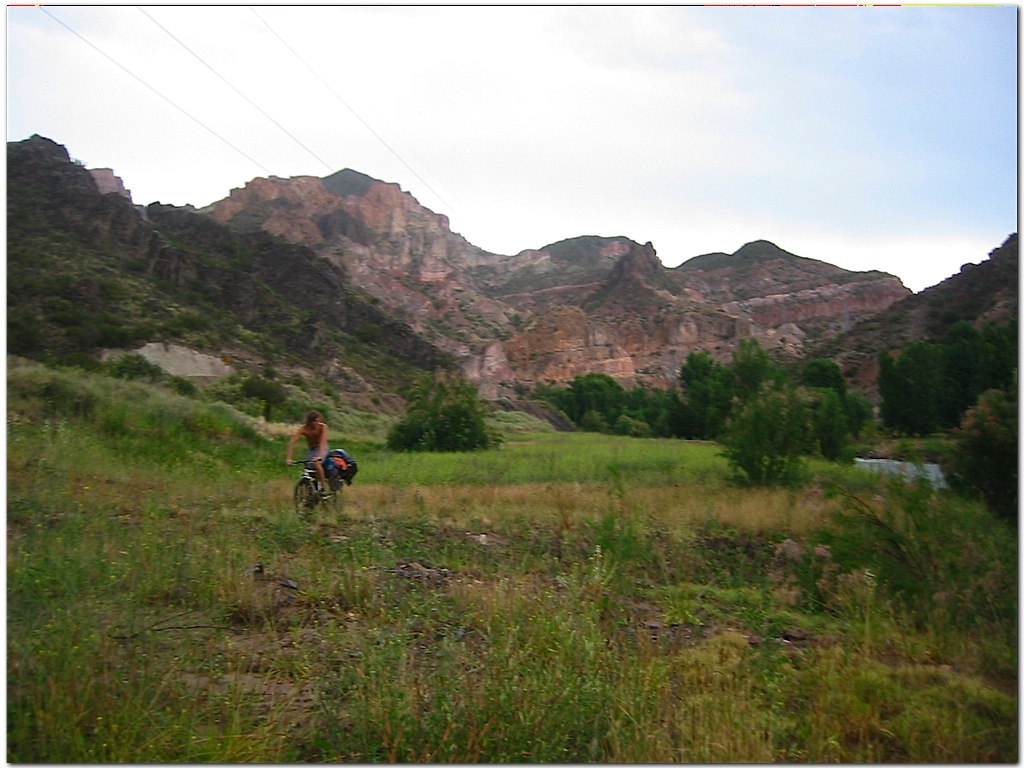
\includegraphics[width=300px]{images/Mendoza_0196.jpg}\\
\textsc{Como en casa.}
\end{center}

Cruzamos a la islita del r\'io, pisando las piedras grandes para estar firmes.
La correntada era fuerte, pero al pasar m\'as baja que nuestra cintura nos
permit\'ia caminar. Yo cruc\'e primero, y, para no mojar dos pares de
zapatillas, ten\'ia que tirarle a Eze mi par. \textexclamdown Con errar un tiro
perd\'ia mis zapatillas en el r\'io y se terminaba el viaje! Pero un poco
nervioso y otro divertido llegu\'e a tirarlas, as\'i que bien calzado Eze
cruz\'o a la islita. \textexclamdown Agua \emph{fr\'ia}! Empezaba justo una
lluviecita fina con sol, ver las gotas iluminadas caer, refrescando, me hizo
sentir en un oasis. Miramos alrededor, dijimos ``esto es lo que queremos'', y
volvimos a buscar troncos para mantener un largo fuego despu\'es de la cena.

Mientras busc\'abamos los le\~nos empez\'o a sonar una tenebrosa y fuerte
sirena, \textexclamdown peor que las de los bomberos! Y qu\'e m\'as pod\'ia
ser que el cercano dique, si ah\'i hay \emph{nada}. Me desesper\'e. Volvimos a
fondo al campamento, lo primero que hice fue subir la bici hasta un lugar alto,
en la cuesta de las piedras sueltas. Estaba asustad\'isimo, porque imaginaba esa
imagen de dibujitos animados en que viene una ola enorme que se lleva todo, y
Eze, m\'as tranquilo, se descostillaba de la risa de s\'olo ver mi cara. Cuando
me tranquilic\'e un poco y entend\'i que no era as\'i de grave intent\'e bajar
la bici, pero no pod\'ia. La hab\'ia subido tanto como nunca hubiera podido:
\textexclamdown era imposible subirla hasta all\'a corriendo a trav\'es de las
piedras sueltas! Ahora no par\'abamos de reirnos.

``\textquestiondown Y ahora qu\'e hacemos?'' El campamento estaba armado.
\textexclamdown Toda esa noche estaba armada! Clavamos una rama a orillas del
r\'io para comprobar que el nivel empezaba a subir, y s\'i; nos exigi\'o
levantar campamento al hundirse lentamente. Todo lo que desarmamos,
\textexclamdown todo!, de nuevo sobre las bicis. Alrededor de las 9 de la noche,
cuando todav\'ia ni hab\'iamos cenado. Triste pero as\'i era la vida. Armamos
todo, y repet\'i la foto que sacamos al llegar mostrando al campamento, pero
ahora enfrente no hab\'ia m\'as que el paisaje y la carpa doblada sobre el
pasto. Por la poca luz y mi mal pulso (entre nervios y cansancio) sali\'o
movida. \textexclamdown Como para olvidar el momento!

Abandon\'abamos nuestro lugarcito saliendo por el barranco ``f\'acil''.
Volvimos unos metros por la ruta para sacarnos una foto con el amigable cartel
``prohibido acampar'' y, \textquestiondown qu\'e encontramos a su lado? Un
camino perfecto para subir y bajar pedaleando al mismo valle. En la emoci\'on lo
pasamos por alto y tuvimos que hacer malabares para transportar la carga.

Empezamos a andar de noche. Est\'abamos un poco cansados por el kilometraje del
primer d\'ia y la subida de hoy, pero no pod\'iamos hacer otra cosa. Salieron
todas las estrellas que pudieron pero la luna no se asom\'o, es la luna nueva
m\'as inoportuna que me haya tocado. Nos iluminaba una humilde linternita
encintada a mi manubrio, entre su poca iluminaci\'on y mi mareo a veces perd\'ia
la l\'inea del camino. \textexclamdown Y el compa\~nero que segu\'ia mi huella
me retaba por no ir por el medio! Poca agua y mucho cansancio para m\'i me
dejaron con baja presi\'on, me costaba enfocar. Cuando la rueda delantera
empezaba a saltar, o el pedal izquierdo a tocar la tierra acumulada en la
banquina, era se\~nal de no estar avanzando por donde quer\'iamos.
\textexclamdown Gracioso por el final feliz! (No nos ca\'imos al r\'io.) Pasamos
un restaurant y un dique, buscando otro cuadrado de pasto donde armar la carpa.
Por el camino, simplemente, no hab\'ia lugar.

Los diques son algo impresionante, sobre todo para estos dos estudiantes de
Ingenier\'ia. Es interesant\'isimo estar sobre esas moles que vibran tanto para
producir, de la fuerza del agua bajando, energ\'ia para las licuadoras y
bombitas de luz de las casas. Qu\'e ingenio.

Volviendo a nuestro problema, a medida que avanz\'abamos buscando un cuadrado
libre de arbustos y fuera del paso, el camino se tornaba m\'as angosto y
des\'ertico.

En el camino encontramos un t\'unel escarbado en la piedra de la monta\~na.
Oscuridad plena adentro, y las linternas con suerte llegaban a iluminar el
rugoso techo. No pod\'iamos saber el largo, ver si era en curvas, si habr\'ia
alguien adentro, si nos chocar\'ian\ldots\ Llev\'abamos una baliza en la parte
trasera de las alforjas para ser vistos. Pero, \textquestiondown y si ven\'ia
alguien medio dormido? Dejamos las bicis sobre el camino pensando todas estas
cosas y, seguramente, exager\'andolas. Por supuesto no nos quedar\'iamos hasta
que saliera el sol, as\'i que volvimos a montarlas y encaramos esos metros. Si
alguien nos tomaba del hombro o nos gritaba cerca, con plena seguridad se nos
deten\'ia el coraz\'on.

Y en plena oscuridad y con los ojos abiertos muy grandes, avanzando lentamente,
se escuch\'o un \emph{``\textexclamdown \textexclamdown ch\'annk!!''} Y\ldots\
\textexclamdown luz! Al hablar lo hac\'iamos murmurando, as\'i que mi alarido,
y su correspondiente eco, se hicieron notar. \textexclamdown Ahora no pod\'iamos
parar de reir! Habr\'ia sensores que al notar movimiento encender\'ian las
luces, igual nunca escuch\'e un encendido tan ruidoso. Aunque no tengo dudas de
que al venir asustado y dormido lo magnifiqu\'e. Cruzamos el t\'unel, no
recuerdo si por el tiempo que demoramos las luces se volvieron a apagar y a
prender, pero ya est\'abamos adentro y advertidos del ruido que provocar\'ian.

Pasada la medianoche y a\'un sin comer, nos sentamos sobre el camino para
descansar un rato. El cansancio molestaba. Comimos bastante chocolate
``Cabsha'', me dej\'o tan asqueado que a\'un me invade una fea sensaci\'on con
s\'olo ver el paquete. Imaginen empezar a andar en bicicleta ya cansados, con
est\'omago vac\'io, y, horas despu\'es, literalmente en medio de una noche y
del camino, esperando un lomo completo con huevo y muchos aderezos, abrir el
pl\'astico del chocolate medio derretido, y comerlo en abundancia.
\textexclamdown Disgust\'o! Pero ten\'ia hambre. Cuando hay hambre s\'i hay pan
duro, pero se lo come igual.

Era la una de la madrugada cuando llegamos al siguiente dique asesino de
acampantes, para cenar los tan esperados capeletinis. Ayer comimos polenta con
tuco, pero esta vez el plato no gozaba siquiera de un saborizante. El precavido
de mi compa\~nero llev\'o atados los le\~nos que \'ibamos a usar en la cocinita
de aquel valle, una salvaci\'on. Todav\'ia me pregunto c\'omo logr\'o
encenderlos: conseguir ramas en estos paisajes no es tarea f\'acil. Los comimos
sentados sobre el gran muro de ese dique, con las piernas colgando sobre la gran
ca\'ida, mirando al vac\'io y el agua caer. Algunos reflectores iluminaban la
obra, era en verdad espectacular.

Hasta el otro dique nos separaba poquito, 8~km creo. Claro que en ese momento
eran mortales para mi, pero no significaban una locura. \textexclamdown La
situaci\'on entera era una locura en realidad!

La suma tiene que dar 118~km para esta noche en que armamos la carpa en una
placita, al lado del dique cuarto. Me tir\'e as\'i nom\'as, con todas las
botellas vac\'ias alrededor, y palm\'e instant\'aneamente agradeciendo ese
pedazo de pasto. ``Prohibido acampar'' en ese parquecito de la entrada,
obviamente, pero de verdad ya no quedaba otra posibilidad. Eran las 3am al
momento de dormirnos. Un d\'ia que no podemos tildar de aburrido.

\subsection*{Mi\'ercoles 5 de Enero}

Alrededor de las diez de esa ma\~nana me despert\'o el calor del sol sobre la
carpa. La micci\'on amarilla intensa revelaba mi deshidrataci\'on. Dolor de
cabeza al moverme y esa cosquilla anterior al calambre constantemente presente
en las piernas confirmaban.

Se despert\'o Ezequiel, y entramos al dique a pedir agua. El gran ruido de las
turbinas nos imped\'ia anunciarnos a dos obreros que trabajaban del otro lado de
la entrada. Entr\'e en la cocina, hab\'ia un dispenser de agua, de los de
oficina. Entre lo que tom\'e en ese momento y las botellas que llen\'e, lo
vaciamos. Ezequiel se preocupaba un poco porque nadie sab\'ia que hab\'iamos
entrado, pero yo me sent\'ia mal, y no me incomodaba nuestro exceso de
confianza. Tom\'e hasta saciarme, y ya me sent\'ia mejor. Cansado f\'isicamente,
pero bien dormido.

Antes del mediod\'ia partimos hacia el Nih\"uil, donde dormir\'iamos aquella
noche. Entre 10 y 15~km no sonaban demasiado, pero unos caracoles en subida en
ripio me terminaron de fulminar. Color verde por el cansancio, me puse verde
claro cuando vi los caracoles desde arriba: \textexclamdown qu\'e bien luc\'ian!
Nuestros primeros caracoles, \textexclamdown y de subida! Las familias sub\'ian
y bajaban en auto, tomando mates y comiendo galletitas o facturas. A nosotros se
nos ca\'ian las babas como a perro. No se imaginan c\'omo empec\'e a valorar el
auto, las comidas, la limpieza\ldots\ y el Viaje.

Llegar a El Nih\"uil fue al principio una liberaci\'on, despu\'es una mala
sorpresa. \textexclamdown Era vac\'io el lugar! Una ciudad que comparo con
Urquiza, pueblo aleda\~no a Pergamino de poca belleza, pero con un dique feo, y
un lago con playas sin sombras donde descansar por detr\'as. Ser\'a que mi
cansancio no me permit\'ia disfrutar, porque diques los hay en todo el camino y
siempre me cautivaron. Pero de \'este, que era tan grande, recib\'ia una pared
de hormig\'on m\'as que un logro de la Ingenier\'ia. Es realmente importante
estar bien an\'imicamente, de eso depende no s\'olo llegar sino tambi\'en
disfrutar el viaje. No pod\'iamos perder tiempo durmiendo ah\'i, pero estaba
moribundo. \textexclamdown Para colmo, los campamentos cobraban como una
hoster\'ia barata en San Mart\'in de los Andes! Y alojaban a gente grande en
auto, no sent\'iamos afinidad.

Almorzamos muy bien, un s\'andwich de milanesa grande y completo, que para comer
tuvimos que salir del restaurantito para que no nos cobren el ``servicio''. No
recuerdo que estuvi\'eramos tan sucios pero es altamente probable. Dormimos una
reparadora siestita en una plaza, y decidimos que volver\'iamos en colectivo a
San Rafael por mi cansancio, pero cuando el chofer se levant\'o de su siesta, me
dijo que las bicis no entraban.

Averig\"uamos que el camino de vuelta era pavimentado, de 20~km hasta El
Desv\'io, un cruce de rutas con parador; y 20~km desde all\'i hasta la Cuesta de
los Terneros, donde empieza una bajada en curvas (de alrededor de 30~km) hasta
San Rafael. 70~km totales. Conclusi\'on: a pedalear para El Desv\'io, que estaba
a mitad de camino de la Cuesta de los Terneros. Ruta desierta, recta y plana;
\textexclamdown m\'as cansadora que los caracoles de ripio y en subida!

Al llegar tom\'e poca chocolatada porque estaba asqueado, y com\'i una
zanahoria; impensable al llegar a un lugarcito donde poder comprar dulces.
\textexclamdown No se asusten que durante el pedaleo, las barras de cereales y
el agua en botellas de 2 litros son moneda corriente! Nos contaron ah\'i que la
noche anterior hab\'ia granizado por la zona y en el dique ni nos enteramos,
\textexclamdown qu\'e buena suerte! Me qued\'e una hora sentado hasta
recuperarme un poco, viendo las chatitas tur\'isticas ir y venir. Era un lugar
de paso, aburrido; y si bien quer\'ia armar la carpa al costado preferimos
seguir hasta la Cuesta de los Terneros y ver menos turismo. Con un poco de
esfuerzo llegar\'iamos, como lo hicimos hasta El Desv\'io.

Pero esta vez era una larga recta en subida suave que no se llega a notar, y uno
avanza entonces frenado sin saber porqu\'e. El paisaje permit\'ia ver por
kil\'ometros la extensi\'on de ruta que faltaba. No hab\'ia carteles, y los
mojones no se acercaban por mucho que pedale\'aramos. En un cruce de caminos
hab\'ia una garita para colectivos, la mir\'e con cari\~no para pasar la noche,
pero ol\'ia muy mal y no nos dejaba c\'omodos.

Ahora estaba verde militar no oscuro, y Eze me habr\'a querido matar, pero justo
antes de la bajada caracoleada de los Terneros, anunciada por un bello cartel,
dije: ``\textexclamdown Basta! Paremos ac\'a porque muero sino''. A esos 20~km
del Desv\'io est\'abamos en la cima de todo el recorrido, el punto m\'as alto.
48~km en subidas este d\'ia en que me duraba a\'un el cansancio de ayer. Y
seguimos subiendo unas dos cuadras para llegar al monumento de San Francisco de
As\'is, donde ahora s\'i dormir\'iamos. Usamos unas 5 o 6 horas en completar
este recorrido. De ah\'i se ve\'ia todo divino, pero no lo pude apreciar mucho
esa tarde. Ezequiel s\'i, recorri\'o y sac\'o las fotos que yo no quise ni pude.

Arm\'e la carpa sin estacas ni sobretecho, sobre un suelo duro e irregular, y
dorm\'i una siesta de una hora en el anochecer. Es bueno dormir, repara r\'apido
la mala onda del cansancio f\'isico. El cansancio persiste pero la mala onda no.
Ezequiel termin\'o con el armado de carpa, y cenamos galletitas con pat\'e, para
no armar el fuego y por mi asqueo. Y ca\'i dormido r\'apidamente.

Antes de la medianoche empez\'o a soplar un ventarr\'on que tumbaba la carpa. Y
nos dimos cuenta: \textquestiondown c\'omo armar la carpa en la punta de un
cerro mendocino? El fuerte viento la mov\'ia golpeando mis pies, despu\'es de un
corto sue\~no me despert\'e sobresaltado. Todav\'ia nos re\'imos porque
empec\'e:

\subparagraph{}\label{ssub:tormenta}
--- \textexclamdown Zequi\'el, zequi\'el! \textexclamdown Se rompi\'o la carpa!
  Zequi\'el, \textexclamdown despertate!\\
\hangindent=1.6cm

Yo no entend\'ia nada, me costaba moverme, y el muchacho no respond\'ia. Al
tocarlo me pregunt\'o para qu\'e lo molestaba; le expliqu\'e, me reincorpor\'e y
segu\'i con la mano todo el per\'imetro que me rodeaba, \textexclamdown estaba
impecable! Algo golpeteaba y entredormido pens\'e que se hab\'ia roto una pared.
Si no era por las estacas despu\'es puestas, en ese momento se desarmaba todo.

Segu\'iamos intentando dormir, y entonces los ruidos se magnificaban. A las 12,
la concentraci\'on de adrenalina en sangre sobrepasaba a la sentida en el valle,
al escuchar la sirena de aquel dique. \textexclamdown Qu\'e d\'ias de descanso
nos tocan! El sobretecho embolsaba el viento y aplastaba la carpa, hasta que se
solt\'o un anclaje y empez\'o a flamear, golpeando las paredes con el gancho. El
ruido nos cans\'o, y entonces lo quitamos y lo entramos para dejar pasar el
viento a trav\'es de los mosquiteros de las paredes, y que ya no se volteen las
paredes. Mientras intentaba volver a dormirme pensaba: ``si viene tormenta y
granizo, pongo la bolsa arriba m\'io y duermo''. Estaba loco, \textquestiondown
c\'omo iba a quedarme quieto si llov\'ia? \textexclamdown Eso me proteger\'ia de
las piedras solamente! Pero de verdad no ten\'iamos otra cosa que hacer. El
fr\'io no molestaba, est\'abamos bien con la bolsa, y por San Rafael no es el
problema a combatir. Importante. Por fortuna no tuvimos que soportar lluvias.

Desde ese momento dorm\'i anestesiado, pero Ezequiel no peg\'o un ojo hasta las
6 de la madrugada; no estaba tan cansado como para dormirse ah\'i. Para colmo, a
las 8:30 empezaron a parar chatitas tur\'isticas, as\'i nos dimos cuenta de que
se trataba de un mirador tur\'istico. En general, a las personas les interesa
hablar con nosotros, pero ese d\'ia nuestra apariencia no ser\'ia de lo m\'as
presentable porque no se acerc\'o ni una persona. \textexclamdown Y les aseguro
que hab\'ia decenas disfrutando de la vista! Yo sentado en un banco de plaza,
escuchando a los gu\'ias hablando de la era paleozoica y de que la Patagonia
llega hasta el centro de Mendoza y no Neuqu\'en. Y Ezequiel se levant\'o un rato
m\'as tarde con cara de pocos amigos. \textexclamdown Mala noche de descanso!

\subsection*{Jueves 6 de Enero}

Reparad\'isimo gracias a mi buen sue\~no, pero todav\'ia un poco cansadas las
piernas, salimos al mediod\'ia de vuelta a la ciudad. Nos separaban de San
Rafael 35 o 40~km de bajada intensa. Foto con la bici posando frente al cartel
que la anunciaba, y a andar. El viento en contra no nos dej\'o exprimir a pleno
el desnivel, \textexclamdown pero c\'omo descansamos! Chupados del viento uno
atr\'as del otro, en bajada, no se pedalea. Y se divierte, jugando con la corta
distancia entre rueda y rueda. Comimos duraznos como desaforados: 2 kg, 15
duraznitos peque\~nos, val\'ian \$1. Dejaron mi cuerpito bailando\ldots

En este frutado desayuno Ezequiel me confes\'o que al momento de despertarlo
antes de esa medianoche, se hac\'ia el dormido, \textexclamdown pero estaba
m\'as asustado que yo! Dice que vio luces de autos entrar y casi muere del
susto, pero despu\'es los vio salir. Yo me acord\'e de ver luces de auto
iluminando las paredes pero por ah\'i lo hab\'ia so\~nado, estaba desmayado.
Ah\'i arriba pod\'ian hacer lo que quisieran, nadie se enterar\'ia. De toda esa
noche charlamos en esta casita de los duraznos, bajo dos bajos y enormes (para
esta zona) \'arboles, desayunando.

\begin{center} 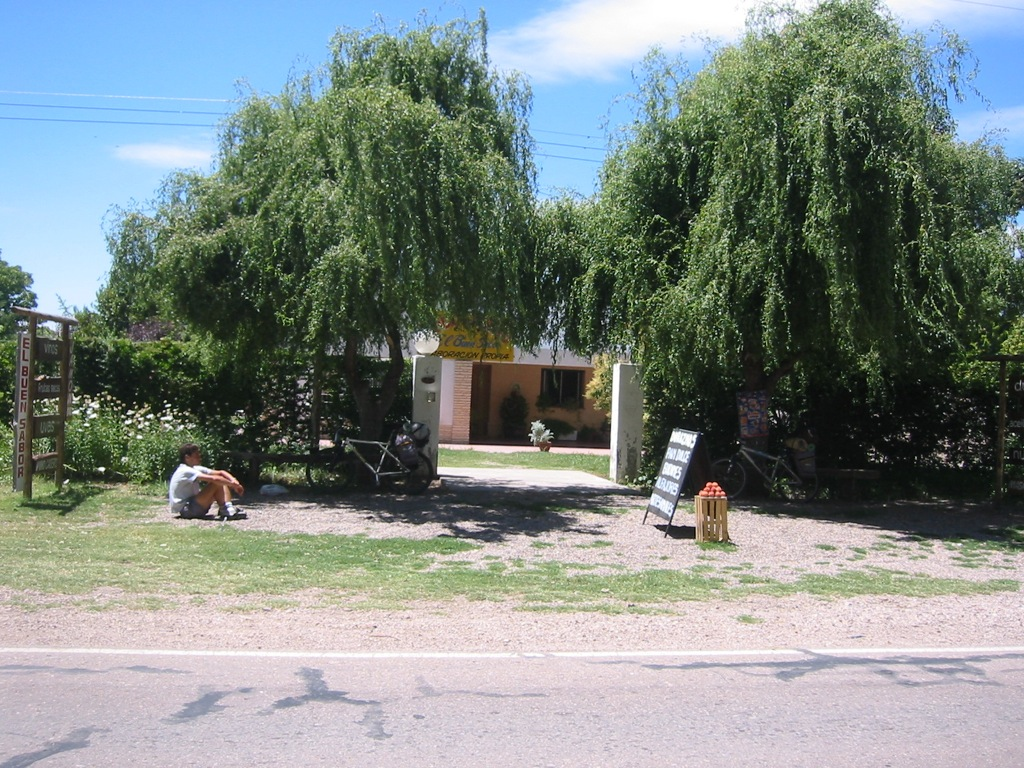
\includegraphics[width=300px]{images/Mendoza_0249.jpg}\\
\textsc{Frutado desayuno camino a San Rafael.} \end{center}

Llegamos a San Rafael, almorzamos muy bien, y decidimos salir para Mendoza en
esa misma tarde porque no encontramos mucho por hacer all\'i. Ten\'iamos
alt\'isimas expectativas, pero pocos fueron los kil\'ometros que las cubrieron
(el ca\~n\'on del Atuel, menos de la mitad del circuito). En realidad todo
estar\'a excelente pero no tanto como esperaba, y, adem\'as, no ten\'ia ganas de
disfrutar porque prefer\'ia siempre dormir. Pero contentos de terminar esta
primera etapa del viaje, y conocer lo que conocimos y hacer lo que hicimos, sin
da\~nos a la salud. Haber llegado.\\

En Mendoza nos cambi\'o la cara. Culminada con \'exito la primer etapa (sin
quemar combustible para cumplirla) nos esperaba esta maravilla de ciudad. De
nuevo sorpresa pero esta vez de la linda, est\'a todo excelente por ac\'a.
Prolija y limpia, buena onda de la gente y mediana de tama\~no, Mendoza capital
est\'a fabulosa. Dejamos los bolsos en un hostal, y recorrimos descansando ayer
y hoy. Era divertido: no ten\'iamos equipaje sobre la bici, ni subidas ni ripio
bajo las ruedas, \textexclamdown y sin embargo no pod\'iamos pedalear!
\textexclamdown Nos costaba avanzar, a\'un en el cambio m\'as liviano!

Al siguiente d\'ia fuimos a la pile de un club, descansamos toda la tarde. La
ducha fue otra salvaci\'on, nunca me dio asco mi piel sucia pero esta vez\ldots\
\textexclamdown mejor no entrar en detalles!

\textexclamdown As\'i que con la frente de nuevo en alto, ma\~nana encaramos el
cruce de la Cordillera en bici! El primer plan era subir por Villavicencio hasta
Uspallata, cruzar por la Ruta 7 a Chile, y volver a Mendoza en colectivo, pero
decidimos subir todo por la 7, volver de Chile hasta Uspallata y\ldots\
\textexclamdown bajar a Mendoza por los caracoles de Villavicencio! As\'i
integramos ambos caminos. Nos lo sugiri\'o un buen lugare\~no interesado por
las bicis cargadas. Ningunos tontos: \textexclamdown as\'i con bajadas
cualquiera viaja!

Estamos ansiosos por entrar en las monta\~nas.

\section{\textexclamdown Empieza el Cruce!}

\subsection*{S\'abado 8 de Enero}

Salimos de Mendoza a Potrerillos, casi descansados, por la ma\~nana.
\textexclamdown C\'omo nos cost\'o salir de la urbanidad de la capital! Hasta el
cruce con la ruta 7 se hizo mucho m\'as largo de lo pensado: 35~km. Luego
tuvimos otros 40~km hasta Potrerillos, pero se ve\'ia de cortina de fondo la
Cordillera de los Andes y nos acerc\'abamos directamente, as\'i que se sent\'ian
bien distinto. Unas horas pedaleando, y logramos meternos en la cortina.

Paramos en una quinta a pedir agua, y un hombre nos advirti\'o del gran calor,
del gran fr\'io, del gran viento\ldots\ ``\textexclamdown Gracias!''
\textquestiondown Pero qu\'e \'ibamos a hacer? Muchas p\'alidas juntas
acompa\~nadas de pocas soluciones. Adem\'as, era lo aceptado al salir de viaje.
Luego, en un parador de barro a la vera de la ruta, paramos a comer un
salad\'isimo pan casero, riqu\'isimo. El lugar divino, atendido por una familia
que vive de esas muy baratas ventas, todos simp\'aticos, y muy prolijito a pesar
de las diferentes sillas y mesas. Bonito. Risas por una tonta ca\'ida al entrar,
un breve descanso, y a seguir.

Llegamos a la bajada a Potrerillos, y en un kiosquito del pintoresco pueblo me
hice ``fana'' de ``Coca-Cola''. \textexclamdown Qu\'e sabrosa se siente al
necesitar l\'iquidos y energ\'ia al mismo tiempo! La disfrut\'e mucho. Llegamos
cansados, por el atrasado y las subidas de la entrada a la Cordillera. El viento
en contra empieza desde el mediod\'ia. Aprendimos r\'apido este detalle,
\textexclamdown pero nunca logramos levantarnos temprano para evitarlo!

Nos indicaron dos campamentos, quedaban bajando por esa calle del kiosco, que
termina en curva cerrada a la izquierda y puente angosto. Los campamentos eran
pasando este puente, a mano izquierda; a mano derecha y tras unos \'alamos
est\'a el dique. Comenzamos a bajar y tomamos r\'apidamente velocidad,
\textexclamdown al describir la curva y pasar por el puente iba tan r\'apido que
no la pod\'ia controlar! Estaba por entrar en sentido contrario una camioneta,
que al vernos pasar hizo se\~nas de luces. \textexclamdown No vi si con cara de
bienvenida o de pocos amigos!

En el primer campamento no entraba ni una carpa m\'as. No dormir\'iamos ah\'i. Y
el segundo estaba tan vac\'io que despertaba sospechas. \textexclamdown Ni el
due\~no estaba! Pero en frente estaban los bomberos, y nos abrieron la
tranquera, asegurando que el due\~no volver\'ia; la idea nos gust\'o. Los
\'arboles estaban marcados con n\'umeros romanos rojos, tenebroso en la soledad.
Pero era perfecto para acampar: sombra en la ma\~nana, colchoncito de pastos
bajo la carpa, enchufes y luz, parrilla, ba\~nos, una linda mesa de
madera\ldots\ \textexclamdown Pero no hab\'ia nadie! No entend\'iamos porqu\'e
la diferencia de gente entre los dos. Nos fuimos a ba\~nar pero los calefones a
le\~na estaban apagados, as\'i que mientras uno se ba\~naba el otro avivaba el
fuego. Cenamos frutas hervidas sobre la original mesa: un c\'irculo de madera
usado para transportar grandes cantidades de cable enrollado. Y, asustados,
pasamos una linda noche. El hombre nunca apareci\'o.

\subsection*{Domingo 9 de Enero}

Desayunamos algo, y seguimos viaje. El due\~no del campamento era de pocas
palabras, as\'i que a\'un pensamos en qu\'e historia esconde este campamento.
Cay\'o esa ma\~nana y le pagamos los servicios.

Ya bien descansados, nos sent\'iamos como siempre, otra vez. Seguimos hasta
Uspallata por la misma Ruta Nacional N$^\circ$7. Bordeamos un poco el movido
r\'io Mendoza, pasaban raftings r\'apido y nos daban ganas de subirnos, debe ser
muy divertido. Con monta\~nas cada vez m\'as altas, nieve apareciendo en pocos
picos, el r\'io siempre tronando al lado y t\'uneles que atravesar (donde se
encajonan los ruidos de los autos y camiones subiendo, estridentes) el
camino fue muy entretenido. Me acuerdo que le contaba a Ezequiel de c\'omo en
los t\'uneles el viento tambi\'en se encajona y lo acelera a uno, una
sensaci\'on emocionante y rara, pero esta vez no atravesamos ni un t\'unel con
buen viento, \textexclamdown todo lo contrario! En alguno nos cost\'o mucho
avanzar.

Unos kil\'ometros antes de Uspallata vimos el cementerio, tendido en la ca\'ida
de una monta\~na. Nos acercamos a las flores para ver c\'omo las manten\'ian en
semejante clima y, claro, eran pl\'asticas. Todas flores de colores, en todas
las tumbas, le daban un toque alegre.

Despu\'es encontramos un barcito donde parar a almorzar, estaba lleno de
camioneros, y todos sus veh\'iculos estacionados alrededor. Son de los camiones
m\'as potentes e inmensos, para cruzar los Andes por Mendoza. Ah\'i comimos un
gran s\'andwich (yo guard\'e la mitad en las alforjas porque ya estaba saciado)
y nos quedamos viendo una pel\'icula c\'omica. La pasamos de diez, los paradores
encantan.

Llegamos despu\'es a la ciudad, y nos instalamos en el primer campamento que
encontramos, pero estaba sucio y casi completamente lleno as\'i que pedimos que
nos devuelvan el dinero. Vuelta a poner el equipaje en las bicis, y seguimos
hasta otro: cerrado al p\'ublico por un festival folcl\'orico. Pens\'abamos
dormir en alg\'un parquecito alquilado (``arrendado'') de una quinta, pero no
encontr\'abamos con qui\'en hablar.

Terminamos preguntando en una iglesia, donde despu\'es de una linda misa y de
idas y venidas de se\~noras a dirigentes y a curas, nos dejaron dormir en la
galer\'ia techada que tienen. \textexclamdown Ni la carpa ten\'iamos que armar!
El piso duro no molest\'o para el buen sue\~no, aunque mi compa\~nero no pudo
decir lo mismo. Los curas y viejas que dirigen divinos, nos despidieron de muy
buena onda, ofreci\'endose para lo que necesit\'aramos. Pensamos que era bueno,
adem\'as, ahorrar los \$12; qu\'e incre\'ible como pasa a otra dimensi\'on el
uso de la plata al viajar as\'i. Yo cen\'e el medio s\'andwich que guard\'e al
mediod\'ia (la mayonesa todav\'ia funcionaba bien), y Eze comi\'o algo liviano.
La noche se hizo para descansar, \textexclamdown nada de andar cocinando!

Nos entretuvimos con una mesa de pool a la que le faltaban algunas bolas
(estaban medio escondidas en un huequito y no las encontramos). Era
divertid\'isimo: uno met\'ia una bola y se escuchaban golpes durante los
siguientes seis minutos. \textexclamdown Despertar\'iamos a toda Uspallata si
segu\'iamos! Tranquilos esta noche, un buen\'isimo descanso. Ac\'a en Uspallata
una curiosidad: hab\'ia rico helado de bananita Dolca en una peque\~na
helader\'ia.

\subsection*{Lunes 10 de Enero}

Ya descansados, casi como nuevos, afrontamos la ruta a Polvaredas.
\textexclamdown Cada vez m\'as Cordillera! Se levant\'o a lo \'ultimo un fuerte
viento en contra, pero 40~km se recorrieron solos entre bajadas y ayudas de la
turbulencia que arrastran los camiones.

En un momento nos pas\'o frenando un grand\'isimo cami\'on chileno, que par\'o
m\'as adelante. Ezequiel se detuvo al lado de su ventanilla y despu\'es el
camionero arranc\'o. Entonces mi amigo se volvi\'o unos metros con una bolsa
naranja grande, sonriendo, y celebr\'o:

\subparagraph{}\label{ssub:camion} --- ``Son buenas para la sed'', me dijo.
\textexclamdown Mir\'a todas las mandarinas que nos dej\'o!\\ \hangindent=1.6cm

La bolsa estaba un tercio llena, as\'i que al sol de esas horas de la siesta
disfrutamos varias, y dejamos otras tantas a la vera del camino. Ten\'ia raz\'on
el conductor: son buenas para la sed. Era una zona donde el r\'io cav\'o un gran
ca\~n\'on y pasa muy por debajo del nivel de la ruta, un lugar precioso y lleno
de distintos colores. Un d\'ia de viaje espectacular, bajo un sol radiante.

Al llegar a Polvaredas era temprano, as\'i que paramos a almorzar. Un gendarme,
luego de explicaciones sobre la canalizaci\'on de los vientos para que siempre
desde el mediod\'ia corra en ese sentido, nos indic\'o un paradorcito donde
comer algo. Charlamos un rato con la due\~na del lugar, tambi\'en le interesaba
escuchar nuestra historia.

A diferencia del sur ac\'a hay poco y nada de mochileros, y llaman f\'acilmente
la atenci\'on. Dicen que es m\'as f\'acil ser ayudado al viajar en bici, porque
los que salen a dedo son vistos como ``hippies'' o m\'as vagos, y la gente no se
solidariza tanto. Nos levanta mucho el \'animo el inter\'es de la gente, nos
llena de voluntad para seguir.

Luego del s\'andwich en este c\'alido parador seguimos a Punta de Vacas, donde
unos gendarmes nos dieron un papel para salir del pa\'is, y para dormir nos
ofrec\'ian una edificaci\'on abandonada, muy oscura y sucia, que ahora usan de
estacionamiento. La otra opci\'on era que caminemos a la vera de un r\'io
perpendicular a la ruta, pero despu\'es de unos 20 minutos de empezar a hacerlo
vimos un cartel que indicaba tres horas (\textexclamdown !) de caminata hasta el
primer campamento, y ya era el atardecer. O no ten\'ian idea del camino (andar
en bici por ah\'i era imposible) o no entend\'ian nuestro viaje, pero volvimos a
Punta de Vacas a tomar una gaseosa para poder seguir hasta Penitentes. El viento
en contra ya nos estaba agotando, es lo que m\'as cansa.

En Punta de Vacas caminamos por los pocos lugares que hay, hasta que encontramos
un contenedor abierto, con un cartel que indicaba que se trataba de un barcito.
Era una preciosura. Al abrir la angosta puerta de doble hoja se entra a una sala
tan larga, angosta y simple como un contenedor puede llegar a ser. Dos personas
charlaban tras una barra y miraban televisi\'on, solos. Cinco mesas
(rectangulares, redondas y cuadradas, ni una similar a la otra) ocupaban el
espacio restante, cada una con sillas de diferentes tipos. Eran en realidad
cinco tipos de sillas, pero mezclados entre las diferentes mesas.
\textexclamdown Una desprolijidad que parec\'ia minuciosamente acomodada!
Pedimos una Sprite de litro, y trajo adem\'as dos vasos de vidrio, cotidianos de
casa de familia. Luego nos tom\'o la foto que le pedimos; es gracioso ver
nuestra posici\'on: tirados sobre las sillas, acostados como si fueran
reposeras, inm\'oviles, forzando la dif\'icil sonrisa mientras apunt\'abamos con
la cara a la c\'amara. Tomamos la botella, nos quedamos un rato m\'as con las
piernas quietas mientras afuera el viento sonaba, y seguimos hasta Penitentes.
Fort\'isimo viento, restaban pocos kil\'ometros pero nos llevar\'ia mucho tiempo
recorrerlos.

Paramos metros antes de Penitentes, en la casa de un vago divino que viv\'ia al
lado de la ruta, con la tranquilidad del pe\'on de campo. Nos ense\~n\'o mucho
de la zona, y nos se\~nal\'o una hoster\'ia donde parar. Ten\'ia adem\'as un
museo de cosas naturales levantado por \'el mismo. Ah\'i vive todo el a\~no, en
medio de la monta\~na, y su \'unica compa\~n\'ia es un guardi\'an y obediente
perro. Tiene electricidad generada por un grupo electr\'ogeno que usa poco.
Prefiere encender una l\'ampara a queros\'en antes que arrancar el motor en
invierno. Muy simple. Nos contaba que de chico sub\'ia con su moto (una Puma),
por el camino de Villavicencio hasta La Cruz, y se tiraba luego con el motor
apagado a dibujar las curvas. \textexclamdown Se le iluminaban los ojos, y
todav\'ia no entend\'iamos lo divertido que puede llegar a ser! Nos volvi\'o a
asegurar, al preguntarle incr\'edulos, que son 365 curvas, ``s\'i se\~nor''.

Paramos en Hotel Ayel\'en, y nos indicaron la Hoster\'ia Ayel\'en, pues no nos
encontraron el suficiente acento alem\'an como para recibirnos. Qu\'e bueno
compartir una cena con ellos, extranjeros de todas las edades prepar\'andose
para escalar el Aconcagua, o gente que ya estuvo intentando y tal vez llegaron,
y estar\'ian contando sus periplos.

No contentos con esto, en la Hoster\'ia nos mandaron a la Guarder\'ia, donde
paraba una familia de pintores y alba\~niles por un trabajo provisorio. As\'i
que por \$10 ten\'iamos habitaci\'on compartida: la m\'as alta de toda la
hoster\'ia y con vista al r\'io (no a las pistas de esqu\'i). Nos duchamos --el
remedio instant\'aneo contra el cansancio y fr\'io que provocan la suciedad-- y
cenamos un lomo completo mirando (esta vez s\'i) a las ahora verdes pistas de
esqu\'i.

Descansamos muy bien.

\subsection*{Martes 11 de Enero}

La ma\~nana del 11 recorrimos poquito las pistas a pie, para salir a la siesta
hacia el Puente del Inca; ya se ve\'ian sus construcciones desde la monta\~na.
Nos distanciaban 8~km de viento en contra, f\'aciles a paso lento. Paramos en el
cementerio del monta\~n\'es, es emocionante. Gente de todo el mundo muerta en
las monta\~nas, con placas llenas de honores sobre tumbas decididamente
rudimentarias.

Al llegar al Puente cruzamos para conocer, caminamos por el viejo hotel derruido
y la capilla, muy interesante y bonito. Fue un d\'ia tranquilo para descansar
piernas y traste, que ven\'ian sufriendo los kil\'ometros que, sino, contin\'uan
acumul\'andose.

Paramos en un camping de por ah\'i, por \$0,50 la due\~na de la casa (en su
patio era el ``campamento'') nos permit\'ia usar la hornalla para cocinar
polenta con leche. Le agregamos salsa, y comimos en nuestra mesa desde la ollita
de aluminio. El fuerte viento la enfriaba tan r\'apido que nos apuramos a comer,
\textexclamdown nos terminamos atorando! \textexclamdown Y para colmo no
llegamos a saciarnos! Qu\'e angurrientos, tuvimos que esperar un rato para poder
acostarnos.

Ducha caliente, a secar el ba\~no, y a dormir pl\'acidamente hasta la siguiente
madrugada.

\subsection*{Mi\'ercoles 12 de Enero}

Nos levantamos a las 8 para visitar las termas del Puente, que s\'olo hab\'iamos
visto. Pasamos media hora relajados en las piletas, nos acostumbramos
r\'apidamente al fuerte olor a minerales. No nos quedamos m\'as porque empezaba
a llegar turismo e incomodaba. Encontramos a un alem\'an en la misma que
nosotros, y mientras nos vest\'iamos le elogiaba su pa\'is pero, sin aceptar
mis palabras, no dejaba de halagar a la Argentina. ``Estando aqu\'i no hay mucho
que a\~norar de Alemania'', explicaba en ingl\'es. Qu\'e lindo, viajar.

Ten\'iamos planeado quedarnos a descansar otro d\'ia en la zona pero\ldots\
\textexclamdown ya conocimos casi todo! Este d\'ia seguimos para Las Cuevas,
pasando por uno de los puntos m\'as atractivos del viaje: el cerro Aconcagua.
Las nubes lo tapaban as\'i que lo imaginamos graaande graande. Ahora tengo otra
excusa para volver a Mendoza: ``\textexclamdown no vi su cumbre!''

Tipo 11 el viento en contra nos empez\'o a frenar, alrededor del mediod\'ia
llegamos y paramos en Las Cuevas, donde ahora s\'i pasar\'iamos el d\'ia de
descanso. Nos metimos y recorrimos, sorprendidos, toda la superficie de una
proveedur\'ia antigua abandonada y derruida. Luego tomamos un gordo chocolate
caliente en la proveedur\'ia antigua de al lado, acompa\~nado con galletitas
dulces y de agua. Un estilo muy alem\'an me pareci\'o el de estos lugares.
Nos atendi\'o una se\~nora de unos setenta a\~nos, ten\'ia un restaurant hermoso
con decoraciones de monta\~na.

Ahora s\'i har\'iamos noche ah\'i, pero\ldots\ \textexclamdown est\'abamos tan
cerca del paso internacional! \textexclamdown Desde ah\'i se ve\'ia el inicio
del t\'unel Cristo Redentor y todo! Nuestro error fue no subir a la imagen del
Cristo por el camino viejo, pues a la 1 de la tarde ya est\'abamos esperando la
chatita que nos atravesar\'ia por el t\'unel (se proh\'ibe, acertadamente,
hacerlo a ciclistas). Mientras esper\'abamos, un gendarme nos indicaba que
nuestras banderitas argentinas no deben lavarse: cuando no dan m\'as, se
cambian. La ansiedad por conocer nos mata continuamente, no podemos estar
quietos. Pasar al otro lado fue un tr\'amite sorprendentemente r\'apido y
f\'acil. Tanto, que olvid\'e declarar la c\'amara de fotos y las bicicletas.

El conductor de la camioneta chilena que nos cruzaba nos dec\'ia que tengamos
cuidado al pedalear por Chile, pues ``\textexclamdown hay muchos conductores
argentinos dando vueltas por ah\'i!'' Entre risas se complet\'o el largo
t\'unel, nos despedimos agradecidos. Fue un alivio el cruce porque no
est\'abamos seguros de poder hacerlo.

\begin{center} 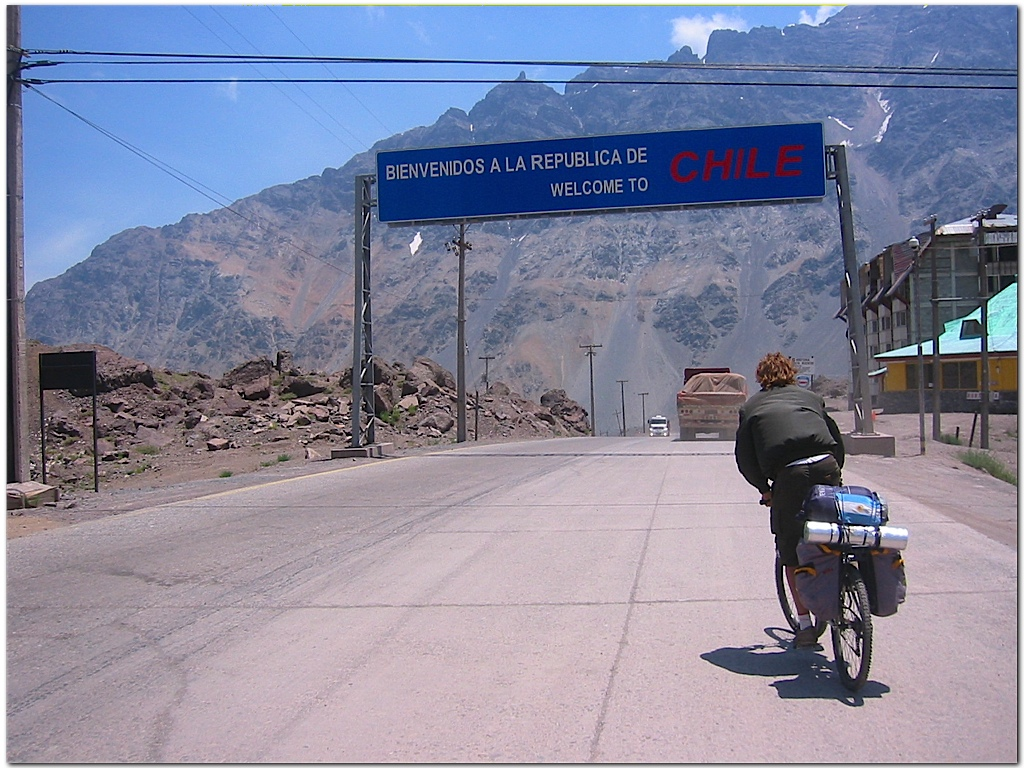
\includegraphics[width=300px]{images/Mendoza_0370.jpg}\\
\textsc{Luego del Cruce, emoci\'on.} \end{center}

Bajamos los caracoles con un fuerte viento en contra, que no nos imped\'ia
adelantar a los camiones. Recordaba de mi primer viaje el olor a frenos quemados
que hab\'ia aqu\'i, pero esta vez el viento nos impidi\'o sentirlo. Baj\'abamos
lagrimeando, entre la emoci\'on y velocidad.

Este fue el momento perfecto del viaje, no puedo describir lo que se siente; fue
espeluznante. A 50~km/h en promedio (entre 70 y 30~km/h) ten\'iamos que apretar
firmemente los frenos para desacelerar la cargada bici, y poder as\'i doblar las
varias y regulares curvas de 180$^\circ$ que conforman este tramo.
Constantemente frenando con dos dedos de cada mano, pedaleando, y zigzagueando.
\textexclamdown Sin ese viento en contra no se si viv\'iamos para contarlo! Las
alforjas empujan fuerte desde ah\'i arriba, se nota mucho. Durante las curvas la
rueda de atr\'as se deslizaba un poco de costado, advirtiendo con un chillido
que no pod\'ia frenar mucho m\'as; eran inyecciones de adrenalina por todo el
cuerpo. Cruzamos en un momento a una pareja en bicis que parec\'ia extranjera,
subi\'endolos. \textexclamdown Tan cargados como nosotros! Los saludamos en el
instante que dur\'o el cruce. No s\'e d\'onde dormir\'ian.

En un momento un cami\'on sub\'ia por su mano contraria, por la l\'inea que yo
iba a usar en mi bajada, de modo de poder abrirse m\'as y no tener que
desacelerar tanto. Por la banquina no lo pasaba, as\'i que pas\'e por mi
izquierda, la parte interna y contraria de la curva, y el hombre pas\'o
tambi\'en por su izquierda, la parte externa. Un cruce \emph{divertido}.

Y en otro momento de esta larga bajada a Los Andes, pero ya en recta,
avanz\'abamos con diferencia de velocidad sobre un cami\'on que m\'as adelante
aceleraba, despu\'es de curvas. Vi que ven\'ia otro cami\'on en sentido
contrario, no lo podr\'ia adelantar; pero quien ven\'ia de frente se abri\'o
cuanto pudo hacia su derecha, y mediante se\~nas con su mano indicaba que nos
dejaba paso al medio. Levant\'e mi mano agradeciendo, y aceleramos pasando por
el medio de los dos camiones: uno bajando, el otro subiendo, y nosotros por el
medio. Emocionante, y peligroso.

La ruta ten\'ia varios cortes por repavimentaci\'on, donde quedaba calzada
\'unica. Al llegar a uno, pasamos justito antes de que cerraran el paso para
permitirles lugar a quienes ven\'ian en sentido contrario, previa autorizaci\'on
del operario, quien avis\'o por handy: ``cruzan tambi\'en dos bicicletas''.
Avanz\'abamos r\'apido por la calzada en buenas condiciones; a nuestra izquierda
ten\'iamos una peque\~na e irregular banquina, y a la derecha una continua
monta\~nita de piedras sueltas que usar\'ian para asfaltar. Porque
demor\'abamos, permitieron el paso de veh\'iculos. \textexclamdown Ver a un
cami\'on subiendo por nuestra misma senda no era de lo m\'as c\'omodo!
Desaceleramos, cruzamos a la calzada que estaban arreglando, y dejamos paso a
quienes sub\'ian. Qu\'e f\'acil es en bicicleta.

Llegamos a Los Andes. Ah\'i nos sugirieron preguntar por Eric, un veterinario
holand\'es, que hizo brutos viajes en bicicleta, y aloja gratuitamente a sus
``colegas''. En la plaza central de un hermoso boulevard muchos nos miraban
sorprendidos y se acercaban a hacer preguntas, pero s\'olo dos de ellos supieron
indicarnos la casa de este hombre. Como justo estaba de viaje tuvimos que buscar
otro lugar donde dormir.

Nos mostraron un hotel ``barato'' pero era hotel, as\'i que seguimos viaje para
ver si encontr\'abamos campamentos. Todav\'ia ten\'iamos horas de luz. Pasamos
San Felipe, luego dos campamentos que no aceptaban d\'olares y me enojaron
mucho, pues quer\'ia parar. M\'as adelante nos indic\'o un hombre con ojos muy
rojos un lugar donde parar, con gestos en el aire nos indicaba:

\subparagraph{}\label{ssub:manan-tiales}
--- Van a ver el cartel: manan-tiales. S\'i: \emph{\textexclamdown
manan-tiales!}\\

Y como todos los chilenos que nos ayudaron, repet\'ia las indicaciones a seguir.
\textexclamdown Era muy gracioso!

Llegamos por fin al prolijo lugar cercano a Panqueue, atendido por una muy
amable y humilde familia. Mientras esper\'abamos al padre, dos chiquitos nos
llenaban de preguntas, estaban admirados. No lo pod\'ian creer: nunca hab\'ian
visto personas viajando en bicicleta. Cuando el hombre lleg\'o, no ten\'iamos
que actuar la cara de cansados, tambi\'en la oscuridad hablar\'ia por nosotros.
Les contamos la historia de este d\'ia, que empez\'o temprano en la ma\~nana en
el ya lejano Puente del Inca, pero no conoc\'ian Argentina. ``Es un lugar muy
lindo\ldots'', y parec\'iamos de otro planeta.

No s\'olo no tuvieron problemas en dejarnos pasar, sino que adem\'as nos
hicieron sentir muy c\'omodos. Ped\'ian s\'olo dos d\'olares por cada uno
contando carpa. El hombre nos mostraba las instalaciones: la pileta de agua
congelada de manantial que podr\'iamos usar ma\~nana, los ba\~nos (ya era hora
de apagar los calefones, pero esperaron a que nos instal\'aramos y
ba\~n\'aramos), las parrillas, etc. Vimos que era un lugar muy familiar, estaba
lleno de autos y tal vez por eso se sorprendieran los chicos por nuestras bicis.

Personas muy serviciales, \textquestiondown c\'omo no voy a enojarme cuando
alguien generaliza diciendo ``los chilenos son antip\'aticos''? Es claro que los
primeros que encontr\'aramos no nos iban a ayudar como necesit\'abamos, pero
depend\'ia de seguir buscando el encontrar buenas personas.

Este d\'ia completamos 125~km y pasamos por alto tres noches (en Puente del
Inca, en Las Cuevas y en Los Andes). Nos cost\'o encontrar un lugar pero
lleg\'o, asegur\'andonos un buen descanso y linda cena. Charl\'abamos de pasar
el siguiente d\'ia en la pileta, descansando, pero al mediod\'ia no pod\'iamos
estar parados en Chile, \textexclamdown hab\'ia que seguir conociendo! Y de
nuevo acortamos d\'ias continuando viaje.

\subsection*{Jueves 13 de Enero}

Bien descansados, la siguiente tarde nos recibi\'o en la ruta, llena de curvas
al principio, con prolij\'isimos montes frutales alrededor, gran sol y cielo
azul. Pero luego el viaje se torn\'o mon\'otono, con suaves sierras y una recta
autopista que se ve\'ia a lo lejos seguir\ldots\ Eso es malo porque parece que
no se avanza, el paisaje parece nunca cambiar. Almorzamos panes caseros y
bananas frente a un comercio del camino, atendido por una mujer que relataba
todos sus problemas al justificar su precio del d\'olar. Me dio un poco de mal
humor.

Ah\'i mismo arreglamos una pinchadura, y un joven nos indic\'o que m\'as
adelante hay un t\'unel prohibido para ciclistas, pero no ten\'iamos otra ruta
alternativa hacia el Pac\'ifico. El problema era si el t\'unel ten\'ia 1~km, 8
como nos dec\'ia el chico, o menos de 1 como otro nos dijo. Ni 8 ni menos de 1,
pero se nos hizo muy corto por el miedo de que fuera verdaderamente largo. Los
autos nos tocaban bocina con raz\'on.

Par\'abamos en La Calera por el viento en contra que nos cansaba, pero era feo y
ni campamento ni hoster\'ia hab\'ia. Paramos a tomar un helado para seguir luego
viaje, pero no nos aceptaban pagar en d\'olares. Una joven madre escuch\'o el
problema y se ofreci\'o a cambiarnos \$600 chilenos por un d\'olar. Linda
actitud.

En ruta a Quillota y luego del helado, pinchamos una rueda trasera sobre un
puente en curva. Una camioneta argentina nos vi\'o arregl\'andola y fren\'o,
baj\'o y se ofreci\'o a llevarnos, pues compart\'iamos destino, Vi\~na del Mar,
a unos 60~km. Pero no cumplir\'iamos con la gran meta, as\'i que decidimos
(Ezequiel decidi\'o, en honor a la verdad) agradecerle y seguir pedaleando
despu\'es del arreglo. El buen hombre se subi\'o sonriendo a la camioneta, y
sigui\'o luego de felicitarnos. Otra buena actitud.

Seguimos acumulando cansancio hasta Quillota, pero era igual, m\'as desprolija y
parec\'ia menos segura, as\'i que, luego de cambiar d\'olares, tipo 7~pm paramos
a comer un gran s\'andwich. Preguntaba la cocinera: ``\textquestiondown Lechuga
picada o de hojas completas?'' \textexclamdown Atenci\'on de lo m\'as
personalizada luego de ganarnos su simpat\'ia! Al principio se enojaba porque
quer\'iamos entrar las bicis, pero le contamos el viaje y que quer\'iamos comida
r\'apida, que necesit\'abamos cuidar todo lo que ten\'iamos (literalmente,
todo), y entonces cedi\'o. Nos sirvi\'o en platos distintos, el m\'io era
amarillo y de ni\~nos, como de juguete. \textexclamdown Ezequiel se
re\'ia cuando saqu\'e la c\'amara para recordarlo! Mis fotos no sirven para
portarretratos ni para concursos, tendr\'e que aceptarlo.

No nos qued\'o otra que seguir a Conc\'on, donde empezar\'ia la costa pac\'ifica
chilena. 90~km este segundo d\'ia, alto promedio en Chile. \textexclamdown En
dos d\'ias cruz\'abamos la Cordillera desde Puente del Inca, y lleg\'abamos al
Pac\'ifico! Tuvo su precio pero tambi\'en su recompensa. El cansancio f\'isico
acumulado es similar al de San Rafael, pero la buena onda ps\'iquica de por fin
estar en los paisajes que esper\'abamos y de la meta (no circuito sino
\emph{viaje}) nos permit\'ia seguir sin perder la sonrisa.

Llegamos a Conc\'on ya de noche. Sobre un puente ped\'i foto a Ezequiel, pero no
quer\'ia sacarla porque no mostraba ni el momento, ni el lugar; no ``dec\'ia''
nada. Pero el recuerdo es lo que para mi vale; por eso me cuesta entender que
mis amigos o hermanos se aburran al mostrarles \emph{todas} las fotos. S\'olo yo
puedo recrear la escena en mi cabeza partiendo del retrato, ya que lo viv\'i.

La gran pregunta era ahora d\'onde pasar esa noche. Una chica de Santiago de
Chile nos dijo que acampaba bajo ese puente, pero es ilegal y si los
sorprend\'ian los echaban. Quer\'iamos comodidad, \textexclamdown era casi el
fin de nuestro viaje! Toc\'abamos puertas para alquilar una habitaci\'on o un
pedazo de pasto pero no nos hac\'ian caso, ya estaba oscuro para pedir ese tipo
de ayudas. Info tur\'istica cerrada y hoteles caros promet\'ian jodernos la
noche de merecido descanso. Preguntando llegamos a una hoster\'ia no muy cara, y
excelente. Ducha, inodoro que necesitaba urgentemente (y que siete cadenazos no
pod\'ian terminar con su trabajo), tres camas (una grande y dos de plaza y
media), m\'as frazadas y {\small TV}, nos daban el descanso y respiro que
necesit\'abamos. Los U\$S 14 m\'as disfrutados del viaje. Un reconfortante
ba\~no y a comer algo, con un leve mareo por hambre y cansancio, que a la vez me
hac\'ian querer salir a festejar y quedarme a dormir.

Caimos en un lugar barat\'in, que por resultar ser de argentinos no jodieron con
la moneda internacional que nos quedaba. La joven pareja nos prepar\'o buenos
s\'andwiches con un chimi-churri ``lo m\'as argentino posible'', y palta, muy
buena. Despu\'es charlamos de lo lindo, nos ense\~naron muchas cosas sobre
c\'omo movernos en Chile. Nos felicitaron por el viaje, y quedamos en volver a
almorzar ma\~nana. Nos ofrec\'ian su casa para dormir, nos ofrecieron internet.
``\textexclamdown Gracias!''

\subsection*{Viernes 14 de Enero}

Hoy nos despertamos temprano para aprovechar el desayuno del hotel, nos tiramos
otro rato a dormir, nos duchamos otra vez\ldots\ \textexclamdown y eran las 12!
\textquestiondown C\'omo parar a almorzar en un lugar conocido, si no
conoc\'iamos la costa chilena?

Comimos unos poderosos alfajores de dulce de leche, y recorrimos toda la
costanera hasta Valpara\'iso. ``La foto'' del viaje fue en una playa de Vi\~na
del Mar; salen tambi\'en los protagonistas secundarios, esos alfajorzotes, y el
oc\'eano, que no se nos ocurri\'o tocar para comprobar que es tan fr\'io como
dicen. La excusa es esta vez para volver a Chile.

Encontramos mucha belleza en esta costanera, donde el mar se ve hermoso con ese
color turquesa, y esas piedrotas angulosas que lo decoran. Como balneario no
deben ser buenos, pero s\'i para ver. Es una ruta com\'un, mano-contramano, que
bordea la serpenteante costa, separada del mar s\'olo por pocos metros de altura
y un guarda riel. Se disfrut\'o much\'isimo de estos descansados 25~km. Una
familia vio nuestras banderas argentinas y nos gritaban saludando y alentando.
Vi muchos Subaru, pero pocos del Turbo, los deben elegir por la nieve y su
tracci\'on integral. Un Porsche en un restaurant coqueto que daba al Pac\'ifico
adornaba el estacionamiento.

Helados de por medio, anduvimos hasta Valpara\'iso, donde preguntamos por la
casa de Pablo Neruda. \textexclamdown Est\'abamos tan cerquita, pero para llegar
hasta all\'a arriba ten\'iamos que desviarnos tanto! Hasta esa avenida de arriba
caminamos diez cuadras de subida muy empinada, con bicis cargadas. Antes tuvimos
que llegar al inicio de esa subida, describiendo entonces una ``V'' corta. Las
cuadras son figurativas para nuestro sistema, porque pasamos s\'olo dos o tres
cruces de calle en esa distancia.

La casa es un sue\~no. Cinco pisos de poca superficie cada uno, habitaciones de
tama\~nos raros, decenas de naturalezas muertas en cada habitaci\'on y pasillo,
adornos de todo tipo, escaleras de diferentes formas y alturas, el mar se ve
desde todas y cada una de las muchas ventanas (hasta desde los ba\~nos), y saber
que Neruda ah\'i escribi\'o y am\'o tantas cosas\ldots\ El artista imitaba al
barco desde su casa, porque si bien le apasionaba el mar, no se animaba a
navegar. Menos mal que estaba esta casa tan divina, porque encontramos
Valpara\'iso muy industrial y poco tur\'istico, a diferencia de la belleza que
muestra Vi\~na del Mar\protect\footnote{Recorrimos poco, luego conoc\'i
descripciones inversas.}.

La vuelta a abajo fue monumental, esas diez cuadras de ahora \emph{intensa}
bajada, pero de calle com\'un, con esos saltitos de brea entre los bloques de
cemento, fueron tremendas. \textexclamdown Con dos dedos en cada freno y con los
otros agarrados del manubrio, necesit\'abamos m\'as manos! No lleg\'abamos ni a
frenar bien ni a sostenernos firmemente, pero de hacer una cosa dej\'abamos
totalmente la otra! La rueda de atr\'as pegaba un chillido en cada saltito,
mostrando que ven\'ia agarrada del pavimento como pod\'ia. Las relativamente
pocas bocacalles nos daban un m\'inimo de seguridad.

Y ahora a comer m\'as alfajores y a la terminal, para volver a Uspallata y bajar
a Mendoza, pero por los caracoles de ripio de Villavicencio. Comprobaremos que
las 365 curvas no son exageraci\'on.

\subsection*{Mail enviado desde Santiago de Chile, pocas horas despu\'es:}

As\'i como llegamos a la terminal, nos subimos corriendo a un bus a Santiago,
porque no hay lugar ni para las moscas en los colectivos, mucho menos directo a
Uspallata desde Valpara\'iso. Llegamos a la estaci\'on y todos nos dec\'ian ``no
hay lugar''\ldots\ \textquestiondown C\'omo pudimos ir tan confiados, como si ya
todo estuviera planeado? Plata para volver en bici no ten\'iamos. Si nos
dec\'ian ``tienen que esperar cinco d\'ias'' probablemente tuvi\'eramos que
comer una vez al d\'ia. Pero el hombre nos dio los pasajes, que despu\'es
descubrimos que estaban mal, entonces volv\'i desesperado a su oficina mientras
Ezequiel cuidaba los veh\'iculos.

\subparagraph{}\label{ssub:Valparaiso} --- Bueno chicos, \textquestiondown pero
ustedes se quieren ir ahora? \\ --- \textexclamdown S\'i, claro! \textexclamdown
Ahora! \\ --- \textquestiondown Ahora, pero ya en este preciso momento? \\ ---
\textexclamdown S\'i, cuanto antes puedan mejor! \\ --- Bueno, entonces
\emph{ya} vayan al colectivo de la plataforma 7 porque los est\'a esperando, les
digo que se demoren 5 minutos. \\ --- \textexclamdown Pero tenemos las
bicicletas! \textexclamdown Todav\'ia no las desarmamos! \\ --- No importa, las
metemos en las bodegas como est\'en.\\ \hangindent=1cm

Corrimos al bus, nos ayudaron a meter las bicis, subimos y arrancamos. No s\'e
como llamar a eso pero les aseguro que as\'i estaba planificado, parec\'ia que
estaban esperando a estos dos viajeros para irse a Santiago y combinar hasta
Uspallata.

En el viaje \'ibamos pensando: ``\textquestiondown Qu\'e pas\'o?'' Est\'abamos
confundidos, no sab\'iamos si hab\'iamos hecho bien en subirnos, mir\'abamos y
revis\'abamos los pasajes, nos pregunt\'abamos si nos habremos olvidado algo
en las corridas\ldots\ \ \textexclamdown Fue raro! Pero funcion\'o como
esper\'abamos.

Al anochecer, al entrar en la Capital ve\'iamos c\'omo son sus colectivos de
l\'inea, nada lindos. Todos viejos, todos iguales, todos amarillos con grandes y
negros n\'umeros cuadrados a los lados que indican la l\'inea. Acostumbrado a
los colectivos porte\~nos, que muchos son un monumento art\'istico, se notaba el
cambio. Y ac\'a estamos, en la gran ciudad, esperando se hagan las 8 am para
salir a Uspallata en un ``R\'apido''.

Comimos en plato y con cubiertos, \textexclamdown ni me acordaba como se usaban!
Los del restaurant, divinos. Era sobre un boulevard muy lindo en
construcci\'on, lleno de conos y carteles naranjas. Una mujer cercana a los
sesenta a\~nos, luego de felicitarnos fervorosamente nos sugiri\'o cenar ah\'i,
y no le err\'o: \textexclamdown hasta las bicis al lado de la mesa nos
permitieron! Era demasiado. Era un lugar muy grande con muchas mesas, de las que
quedaban dos libres. Todo el restauran se daba vuelta para ver a los dos
delirantes maniobrando las m\'aquinas cargadas, para dejarlas cerquita pero sin
que molestaran al pasillo. Al lograr sentarnos, transpirando de la verg\"uenza,
nos sugirieron que cambiemos de mesa para estar m\'as c\'omodos. ``As\'i est\'a
bien\ldots'' Pero con \'animos de ayudarnos nos levantaron y llevaron a otro
lugar, de verdad m\'as c\'omodo. Escuchaban con atenci\'on sobre el viaje, todos
se sorprenden y nosotros tambi\'en porque ya pasamos los 700~km recorridos.
\textexclamdown Es que hicimos 230~km en Chile, en dos d\'ias! Vamos a un
promedio de m\'as de 60~km por d\'ia desde que salimos, mi traste ans\'ia un
sill\'on donde apoyarse.

Nos vemos en pocos d\'ias, luego del festejo en Mendoza de haber \emph{cruzado
la Cordillera} a pedal. Nos morimos de risa por el tono con que decimos
``\emph{cruzar la Cordillera}''. \textexclamdown Suena gordo y lo exageramos a
prop\'osito!

Ac\'a el argentino que atiende el cyber (que no para de decir ``boludo'',
necesita volver a su pa\'is) nos dice que no hay fernet por Chile, as\'i que nos
sacaremos las ganas en Argentina. Estamos totalmente libres de toxinas despu\'es
de dos semanas transpirando y tomando agua de monta\~na. \textexclamdown Pero no
ser\'a por mucho tiempo!

A medianoche salimos del cyber, y, paseando por una plaza central, nos
encontraron dos chicas de unos 25 a\~nos, que caminaban junto a un peruano de
similar edad, completamente ebrios. Empezaron a charlar, se re\'ian, hac\'ian
chistes\ldots\ \textexclamdown Hac\'ian preguntas, y no dejaban tiempo
suficiente para que respondi\'eramos! Ezequiel no puede recordar lo siguiente
sin re\'irse: el hombre quer\'ia que dij\'eramos que ellos (Per\'u) eran los
m\'as grandes jugando al f\'utbol. Nosotros le fundament\'abamos porqu\'e no lo
quer\'iamos decir pero \'el insist\'ia, todo lo que quer\'ia era escuchar eso.
Sin mucho sentimiento le asentimos: ``s\'i, ustedes son los m\'as grandes''.
\textexclamdown Despu\'es de todo era irrelevante! Al escucharlo dibuj\'o
sonrisa, se qued\'o tranquilo, y se fueron. \textexclamdown Simplemente lo
quer\'ia escuchar! Un encuentro raro y divertido. Ezequiel nunca lo recuerda sin
re\'irse.

Hablando de sin-sentidos, qu\'e guachos somos varios argentinos, despu\'es ``nos
queremos llevar bien con `los chilenos' ''. Un verdulero de Uspallata nos dijo,
concluyendo entre otras cosas: ``\textexclamdown y lo bien que los tratamos, a
los hijos de p@\#\&!'' \textquestiondown No se dan cuenta? Y la mujer del
restaurant de Conc\'on, que ``nos odian porque\ldots\ \textexclamdown somos
mejores!'' Y sonrisa. Cara-rotas es poco decir. Brutos.

\textquestiondown Cu\'antos chilenos nos odian? \textquestiondown S\'i?\\
\indent \textquestiondown Y qui\'enes, por ejemplo? \textquestiondown S\'i?\\
\indent \textquestiondown Y porqu\'e? Empezar por casa es m\'as f\'acil que
justificar el maltrato, me parece.

Del encuentro con los tres muchachos de fiesta seguimos paseando por el Centro.
Pasamos por edificaciones hermos\'isimas, muy bien iluminadas, imponentes,
tendr\'an una historia digna de conocerse.

Caminamos por una linda y prolija peatonal donde, tom\'abamos un helado parados
con las bicis entre las piernas, para cuidarlas. Pasaron dos o tres hombres de
unos 40 a\~nos que hablaban en ingl\'es, no se notaba que hab\'ian tomado sino
por c\'omo hablaban. O tal vez lo hac\'ian por la libertad de saberse en la otra
punta del mundo donde no todos hablan ingl\'es. Pero empezaron en voz alta:
``\'estos son verdaderos ciclistas, nosotros somos gallinas''. Yo me di vuelta,
sorprendido, con una sonrisa que les habr\'a mostrado que los escuchaba. ``Eso
es viajar en bicicleta: con los bolsos, la carpa, la bolsa de dormir\ldots\ \
\textexclamdown Como nosotros cualquiera es ciclista!'' Lo hac\'ia de muy buen
modo, con mucho humor, ten\'ia ganas de contestarles para empezar a charlar,
pero as\'i como aparecieron a mirar las alforjas y banderita se volvieron a ir.

Nos dec\'ian lo mismo que los viajeros de San Rafael, pero ahora no podemos
pensar que fuera por compromiso o para ayudarnos durante una \'aspera subida,
empapados en transpiraci\'on como aquella vez. \textexclamdown Era su
conversaci\'on! Es evidente que no se necesita privarse de comodidades por
d\'ias para ser ciclistas. Pero aparentemente a ellos les interesaban los viajes
largos y les gustar\'ia hacer uno, tal vez no se animaran a decir ``chau vieja,
vengo en tres semanas''. Sino, \textquestiondown para qu\'e decirlo?
\textexclamdown Con decir ``a estos dos les chifla el mo\~no'' bastaba! O
simplemente dos tipos que tienen ganas de pedalear, ni locos ni Ciclistas con
may\'usculas. No hay que quedarse, hay que salir, cada uno en la medida que
pueda y quiera. Pero hacerlo cuando se puede.

Otro pensamiento para m\'i raro: una mujer en Quillota no dejaba de pensar que
estamos locos. Le explic\'abamos que no, que era el modo que eleg\'iamos para
conocer. ``\textexclamdown Pero hay que tener ganas, ehh!'', conclu\'ia.
Baldeaba su vereda mientras conversaba. Tomamos de su agua, y seguimos
pedaleando despu\'es de saludar y agradecer. Tal vez sea este tipo de reacciones
las que me llevaron a querer escribir los relatos. Mostrar la simpleza y
humanidad (no super-heroismo) que hay en nuestras ganas de viajar en bici.

Volvimos a la Terminal de Santiago por ese boulevard tan lindo en
construcci\'on. Tanto desorden provocado por las mejoras, la poca luz, y mi
cansancio y sue\~no, hac\'ian que empiece a enfocar dificultosamente. Sin
embargo, me acuerdo como si una cinta lo estuviera proyectando sobre mi frente.
Parec\'ia de mentiras, parec\'ia un jueguito de computadora. En la capital
chilena, pedaleando en contramano (no hab\'ia tr\'ansito) a trav\'es de
m\'aquinas amarillas, conos rojos luminosos, carteles de diferentes colores,
tipograf\'ias y modos de colgarlos, gente en la noche de ese Viernes y madrugada
de S\'abado\ldots\ Esos momentos tan especiales hacen que vayamos muy r\'apido,
ya que no hay grandes distancias por recorrer. Entonces yo lo segu\'ia a mi
amigo, que con sus alforjas y banderita flameando era como un se\~nuelo, y me
divert\'ia viendo el paisaje moverse cercano y r\'apidamente. De esos momentos
que se graban en la memoria.

Llegamos a la Terminal, y tuvimos que mostrarle los pasajes al guardia para que
nos dejara pasar. La cierran, pero no para todos. Nuestra noche no se hizo muy
larga: pudimos dormir bien en el piso porque est\'abamos cansados, aunque no
mucho tiempo como necesit\'abamos. Nos despertaban para limpiar, y nos
volv\'iamos a estirar en el suelo. Ni escuch\'abamos cuando quer\'ian
levantarnos, entonces sent\'iamos que nos pateaban con poca tranquilidad en la
planta de los pies. \textexclamdown Al despertarnos ve\'iamos a la se\~nora que
trabaja en la limpieza con cara de pocos amigos, y a los dem\'as viajeros
mir\'andonos conteniendo la risa! La luz del lugar nos volv\'ia a encandilar,
hasta que encontr\'abamos otro lugar y posici\'on donde seguir durmiendo. Lo
hac\'iamos contra las puertas de las boleter\'ias, para que al abrir nos
despertasen y tomar entonces el colectivo de esa madrugada.

\section{Las 365 curvas de Villavicencio}

\subsection*{S\'abado 15 de Enero}

Subimos a nuestro bus despu\'es de embalar las bicis, llegamos a Uspallata
despu\'es de ver toda la ruta que hab\'iamos recorrido, ahora de vuelta y a
trav\'es de la ventana. Pod\'iamos ver en todo el viaje al r\'io y las v\'ias,
que no pod\'iamos apreciar desde nuestro lado al bajar contra la monta\~na. Y
as\'i, mirando la extensi\'on recorrida, dije lo que nunca se me hubiera
ocurrido pensar: ``\textexclamdown hay que tener ganas, ehh!''. \textexclamdown
Pero nunca faltaron! (Casi.)

En Uspallata comimos bien y salimos para Villavicencio, que, a no mucha
distancia de bajada y con poco viento por la zona, promet\'ia ser una frutilla
del postre, un fin de viaje relajado. \textexclamdown El broche de oro!
Villavicencio estaba a 70~km al final (m\'as 50~km a Mendoza capital) pero todo
bajada y sin viento\ldots\ Villavicencio estaba a 70~km con mitad subida, mitad
bajada, y fuerte (el primer d\'ia, pues al final nos tomamos dos para
completarlo) viento en contra. \textexclamdown El clima de viajeros en bici
volver\'ia, nuestro viaje no terminaba! El broche de oro requer\'ia exigencia.

Demor\'abamos la salida. Tomamos helado, paramos en una arboleda\ldots\
despu\'es nos esperaban aridez, sol y condiciones desfavorables para mantener
una velocidad media. Subimos a un promedio de 6~km/h entre el cambio liviano y
caminatas. El viento nos frenaba mientras los serruchos nos quitaban el
equilibrio. En las subidas empinadas la rueda delantera se levantaba al mover
los pedales, impidiendo a la trasera traccionar. Tomamos toda el agua que no
usar\'iamos hasta Mendoza. \textexclamdown Y todav\'ia no est\'abamos a medio
camino de la Reserva! Peligroso, aunque de vez en cuando cruz\'abamos personas.

Cay\'o la noche, pero la luna estaba creciendo as\'i que hab\'ia luminosidad.
Seguimos por unas eses en subida que recordaban a esa subida de San Rafael:
mientras se piensa que no se puede estar m\'as alto, se sigue subiendo y las
eses se prolongan, y los cerros siguen cortando la visi\'on del camino de
subida\ldots\ \textexclamdown Y charl\'abamos de qu\'e hacer en caso de que se
nos cruzara un puma! ``Hay que hacerse el grande con los brazos, y quedarse
quieto''. \textexclamdown Serenidad es lo que faltaba!

No encontr\'abamos ni donde tirar la carpa hasta una cruz que hay por ah\'i.
(``La Cruz'', un mirador de la pared Norte del Aconcagua.) No entend\'iamos
que fuera un mirador: \textexclamdown tanto tiempo vimos ese paisaje durante la
lenta subida! Era el punto casi m\'as alto antes de empezar la --m\'itica para
nosotros-- bajada de Villavicencio de unos 20~km y 365 curvas. Era de noche y
est\'abamos de verdad cansados, con poca agua y hambrientos. Decidimos no s\'olo
descansar sino adem\'as esperar a que saliera el sol, para deleitarnos de verdad
con esa bajada tan deseada, que en planes ya deber\'iamos haber bajado pero
todav\'ia ni siquiera ve\'iamos.

Mientras arm\'abamos la carpa pasaron dos autos. Hicimos se\~nas a cada uno para
que frenara y por favor calmara nuestra sed. Uno pas\'o despacito mirando, pero
no debe haberse animado. \textexclamdown Estaba oscuro! El segundo, una
``Traffic'' conducida por una joven pareja, fren\'o a preguntar algo y nos
dej\'o dos litros de agua despu\'es de contarles un poco nuestro viaje.
Impresionante. La chica as\'i estaba, impresionada. Nos salv\'o esa noche y el
siguiente desayuno, pero, m\'as que nada, la salud y bienestar para el siguiente
d\'ia. \textquestiondown Qui\'en viaja en auto con una botella de dos litros
atr\'as, llena de agua? Otra casualidad que necesit\'abamos y nos solucion\'o un
importante problema. Eran dos chicos de Capital Federal, que subieron todo sin
saber c\'omo era y\ldots\ \textexclamdown se les hizo largo! No sabemos c\'omo
se les puede hacer largo este camino. Los primeros eran amigos y siguieron
viaje, pero ellos, cansados, pasaron la noche tambi\'en cerca de La Cruz.

Comimos algo, y nos tiramos a dormir. En medio del silencio cordillerano, Eze
pregunt\'o: ``\textquestiondown Qu\'e estar\'an haciendo los muchachos ahora?''
Y tambi\'en empec\'e a pensar en aquello. Era un s\'abado a las 10:30 de la
noche. ``El abuelo'' se estar\'ia ba\~nando para recibir a los dem\'as en su
casa. El ``pelado Queen'' estar\'ia poni\'endose desodorante para caminar al
centro. El ``Otto'' estar\'ia afeit\'andose con la canilla abierta.
\textexclamdown Las cosas cotidianas que cada uno de nosotros hace un d\'ia como
ese a una hora como esa, y que sin embargo nos eran tan lejanas y fuera de la
realidad, que ni siquiera las a\~nor\'abamos! Creo que esa noche mis viejos
estaban de gala en el casamiento de un sobrino. Es rar\'isimo e
interesant\'isimo pensar en esos mundos distintos pero paralelos. Nosotros
est\'abamos echados como nos hab\'iamos echado en una carpa, en una noche
ventosa en el medio de un cerro, habiendo cenado un paquete de ``Melbas'' y un
alfajor ``Milka''. \textexclamdown Habiendo hablado de hacernos los grandes con
los brazos ante la presencia de un puma!

Estos pensamientos no nos impidieron dormir profundamente.

\subsection*{Domingo 16 de Enero}

Nos levantamos a la ma\~nana siguiente, y desayunamos las sobras de la cena
(galletitas ``Melba''). As\'i que muy bien nutridos, a las 9:30am, levantamos
campamento y salimos en las bicis.

\textexclamdown Impresionante! El viento hab\'ia rotado y ya pod\'iamos pasar
los 20~km/h. Despu\'es de un d\'ia a 6~km/h significaba un reconfortante alivio.
No s\'olo eso: a 35~km/h los serruchos nos acalambraban los dedos, y llegamos
hasta la verdadera \'ultima subida. Desde ah\'i empezaban \emph{los caracoles},
de ripio, piedras y marcados serruchos.

Fue divino, \textexclamdown se demor\'o pero lleg\'o el premio! Desde ah\'i
arriba se ve\'ia el suelo de Mendoza, la lejana planicie tras las monta\~nas. La
ruta que tomar\'iamos desde el Hotel Villavicencio a la Capital parec\'ia desde
ah\'i una pista de aterrizaje. Los caracoles son incontables curvas (si uno las
baja) de ripio que pasan por varios cerros, as\'i que tienen variadas formas,
pendientes, y peraltes, a diferencia de los regulares y asfaltados caracoles de
bajada a Chile. \textexclamdown Una deliciosa prueba para los ciclistas! Era
lindo ver c\'omo la bici iba de lado a lado de la senda, mientras uno no variaba
la direcci\'on, as\'i de sinuoso era el camino. Otra vez, \emph{espeluznante}.
Nunca viv\'i algo tan entretenido sobre la bici, por tiempo tan prolongado. Eso
es lo que lo hizo \'unico.

\begin{center} 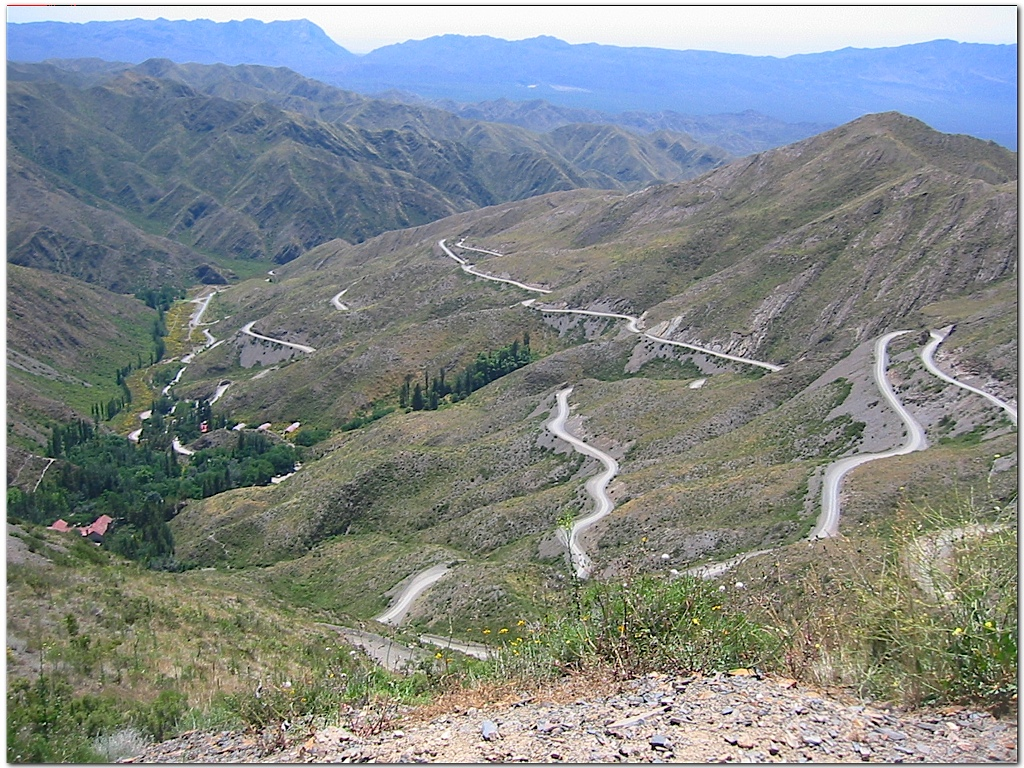
\includegraphics[width=300px]{images/Mendoza_0450.jpg}\\
\textsc{El impredecible camino.} \end{center}

La sensaci\'on de que un motor no nos deja de acelerar, de llegar a 45~km/h a
frenar antes de las (cerradas) curvas --que no se ve c\'omo sigue el camino si
son a la derecha--; la senda all\'a abajo, vi\'endose serpentear y esperando
nuestro paso; el dedo \'indice en los frenos mientras los otros cuatro se
aferran fuertemente del vibrante manubrio; las cubiertas escarbando la tierra
intentando desacelerar\ldots\ pocas veces (por suerte) la delantera queriendo
seguir derecho mientras se intenta doblar, \textexclamdown adelantando
apretadamente a un Honda azul (dos veces), que despu\'es encontramos en el
Hotel! Fue algo verdaderamente emocionante.

Llegamos al hotel con sonrisas que no cab\'ian en nuestra caras, y nos tomamos
la foto junto a las bicis. En el ba\~no, un hombre nos pregunt\'o si hablamos
ingl\'es. Era californiano, \'el bajaba con su esposa y un chofer en el Honda,
visita Argentina para recorrer vi\~nedos. Estaba interesado en nuestro viaje:
``\textquestiondown a d\'onde van con tantos bolsos?'' Tambi\'en se alegraba de
que no tuvi\'eramos los caracoles de subida. ``Bueno, si no contamos todo el
\emph{largo} d\'ia de ayer, entonces no, \textexclamdown no tuvimos subidas!''
Risas, y al restaurant a festejar.

El men\'u era con plato de entrada, principal y postre. Todo por \$20, como dos
noches en un campamento caro. \textexclamdown Buen\'isimo! Nos sentamos, pero
por nuestra apariencia de zaparrastrosos no combin\'abamos ni con el perro del
lugar. \textexclamdown C\'omo se disfrutan las comidas de viaje! Se come porque
de verdad se llega a necesitar, y si adem\'as es rico\ldots\ \ Primero empanadas
y un ``aderezo picante'' para el pan; despu\'es chivito con ``batatas a la
miel'', y flan con dulce de leche de postre. \textexclamdown La pasamos mal
estos \'ultimos d\'ias! Comimos hasta las migas de las dos paneras, y despu\'es
caminamos los 200m hasta el Hotel.

Hay much\'isima vegetaci\'on en este punto, y hac\'ia d\'ias que no ve\'iamos ni
un \'arbol. Subimos al mirador para ver al hotel con la misma perspectiva que en
las etiquetas de cada botella, un cuento de hadas estar ah\'i. No sab\'ia que
exist\'ia. Desde entonces, cada vez que veo esa imagen, sea en una botella o en
un cami\'on por la ruta, se me imposibilita no recordar ese d\'ia de sol.
Invariablemente, siempre, en cualquier momento y lugar. Conocimos finalmente la
capilla, y volvimos al restauran a la hora de la siesta, para dormir un poco
sobre el pasto y bajo la sombra de un gran \'arbol. No quer\'iamos llegar a
Mendoza y dar por terminado el viaje.

Apareci\'o un hombre de Esquel, de unos 55 a\~nos; reci\'en empezaba su viaje en
bici desde Mendoza. Planeaba cruzar por San Juan a la Serena (Chile), bajar
bordeando el Pac\'ifico hasta Vi\~na del Mar, y volver a la capital mendocina
atravesando el Cristo Redentor. Un \emph{gran} viaje. Su bici era muy com\'un,
casi de paseo, y llevaba menos carga que Ezequiel o yo. Una simpleza infinita,
no s\'olo por la imagen pero tambi\'en por su modo de pensar y hablar. Charlamos
un buen rato, nos dej\'o el tel\'efono para visitarlo si sale nuestro viaje del
2006. Le cambi\'e mi botella grande de agua por una chiquita que \'el tra\'ia,
as\'i llega a La Cruz sin deshidratarse. Nos despedimos dese\'andole lo mejor, y
seguimos viaje a Mendoza.

Una ruta aburrida y derecha luego de pocas emocionantes curvas ahora
pavimentadas, pero todo de bajada. Un promedio cercano a 35~km/h la primer hora.
Estamos acostumbrados a movernos a 15~km/h, pero llegamos a 63~km/h en este
asfalto. Y era en una curva no muy abierta, y se escuchaban las cubiertas
silbando; \textexclamdown piel de gallina y sentida sonrisa! A medida que la
recta avanzaba, solita bajo nuestros quietos pies, el clima cambiaba
perceptiblemente. Mayor temperatura, mayor humedad, y un sol m\'as intenso y
pesado. Cuando paramos a tomar el agua nos sorprendimos de su temperatura,
estaba no tibia sino \emph{caliente}. Toc\'abamos los metales, el manubrio, la
cubierta; estaban \emph{calientes}. \textexclamdown Impresionante! A volver a
transpirar pesadamente.

Culminamos el viaje en Mendoza Capital, \textexclamdown de nuevo
esta gran ciudad! Quisimos parar en la hoster\'ia amiga pero estaba llena.
Hab\'ia gente pero no nuestros conocidos, les dejamos saludos y las buenas
noticias. Gastamos despu\'es el tel\'efono buscando hoster\'ias, hasta que nos
interrumpi\'o un hombre: ``\textquestiondown necesitan hoster\'ia?'' Las cosas
siempre terminan bien por ac\'a. Barata y con todo lo que necesitamos. El hombre
nos ofrec\'ia ``pastelitos mendocinos'', cuando vimos los tradicionales
bizcochos nos morimos de la risa. Nos quedaremos hoy, ma\~nana iremos a este
club que ya fuimos, le dar\'e un beso a la familia mendocina y tomar\'e el coche
cama a Mar del Plata. Mejor no puede ser todo. \textexclamdown Imagin\'andolo no
llegar\'ia a tal gozo!

Content\'isimos de terminar el viaje de 900~km aproximados, sin contratiempos ni
momentos feos, conociendo mucho, y casi la totalidad de los kil\'ometros
maravillados por alguna cosa de la regi\'on. Y de hacer estos \'ultimos
caracoles que de verdad me maravillaron, agradecido de por vida. Todo eso, sin
golpes ni heridas. \textexclamdown Y bastante vivos!

Dormimos muy bien en camas c\'omodas, con s\'abanas. Nos ba\~namos, lavamos la
ropa en el mismo lugar. Nos re\'imos sin parar. Cenamos pizza en un restaurant,
donde no nos cost\'o hacernos amigos del mozo, que nos trajo de postre dos
mitades de durazno con crema con una muy sugestiva presentaci\'on.\\

\subsection*{Lunes 17 de Enero}

Fuimos a un club para atenuar el choque con el calor h\'umedo. Nos duchamos
cuanto pudimos, comimos helados, y recorrimos. Cen\'e en un restaurant con mis
t\'ios, previa pizza con Ezequiel que prefer\'ia recorrer la ciudad a pie.
Compr\'e el pasaje a Mar del Plata, que por suerte consegu\'i para el Martes
porque de nuevo me confi\'e: fue dif\'icil conseguir lugar. \textexclamdown Me
tuve que conformar con un coche cama sin paradas! De nuevo de lujo, como el de
vuelta de Bariloche. Me gusta gastar los \'ultimos ahorros en un lujo
caprichoso.

Saldo para la bici: 3 c\'amaras pinchadas, una rueda torcida y por tanto freno
gastado, mi porta paquetes desoldado en dos puntos (\textexclamdown
Villavicencio!), y cadena muy seca. Un rayo cortado. \emph{Nada}.

Saldo para m\'i: una visi\'on m\'as simple de todas las cosas.

\newpage
\thispagestyle{empty}

\chapter{Europa}
\begin{flushright}
\item \emph{\small ``Al viajar, uno aprende m\'as de su propio pa\'is que del lugar que est\'a visitando.''  \\
An\'onimo}
\end{flushright}
\section{Preparativos}

Antes del viaje y luego del pedaleo por Mendoza, en el primer cuatrimestre del
2005, estaba cursando en Buenos Aires el Ciclo B\'asico para Ingenier\'ia.
Despu\'es de la generosa invitaci\'on de mi viejo a visitar Europa, descripta
en la introducci\'on, empec\'e a enviar mails a mis t\'ios espa\~noles (viven
en el centro y norte de Espa\~na), a amigos (del sur espa\~nol) y a un amigo
de pap\'a que vive en el centro de Alemania, en G\"ottingen, y se llama Gustavo.
Iba a ir unas semanas, como a cualquier viaje, pero desde que empezaron los
mails comenzaban las sorpresas.

Los espa\~noles me recib\'ian con gusto, mi t\'io se tomaba vacaciones ese
verano (en Julio) para mostrarme \emph{todo} lo que quer\'ia. Y Gustavo me
contest\'o que si me quer\'ia quedar seis meses, que simplemente lo hiciera:
su casa estaba abierta; y me describ\'ia un poco (\textexclamdown \emph{muy}
poco, aunque pareciera tanto!) c\'omo ser\'ia mi vida en Alemania, queriendo
ocuparse de que no me aburriera un minuto. \'El no entend\'ia: \textexclamdown
yo curso ac\'a! \textexclamdown Estudio! De todos modos reenvi\'e ese mail a
mis viejos, para que agradecieran ellos tambi\'en la gran invitaci\'on. Los
dos contestar\'ian que era una locura, pero ver\'ian en Gustavo una hermosa
actitud.

Llegu\'e de la facultad al mediod\'ia, y me esperaban mails de ambos. El de
mam\'a me descarril\'o. Ella me iba a extra\~nar mucho, pues era una
oportunidad que no pod\'ia perder. Que lo pensara. Que irme con el ciclo
b\'asico terminado era una buena idea. Pero no cerraba ah\'i el mail porque ya
me suger\'ia en el mism\'isimo mensaje que llevara una raqueta porque a Gustavo
le gusta jugar al tenis, que disfrute de los bosques de alrededor, y de lo
amigable de la gente de su barrio. \textexclamdown Y yo esperaba recibir
solamente un ``qu\'e lindo gesto el de Gustavo''! Emocionado y todav\'ia
incr\'edulo, le\'i el de pap\'a. Avalaba lo que dec\'ia mam\'a, me autorizaba a
tomarme medio a\~no de vacaciones (\textexclamdown con tanto estr\'es lo
necesitaba!), y me daba libertad de volver cuando quisiera, sea a los 2, 3 \'o 6
meses.

Imaginen por d\'onde volar\'ia mi cabeza esos tiempos, que fui a rendir el
\'ultimo parcial con el dinero del pasaje en el pantal\'on. Le ped\'i
compa\~n\'ia a un amigo que terminaba de rendir conmigo, \'el no pod\'ia creer
que rindiera y caminara tranquilo con eso\ldots\ \textexclamdown En realidad
yo tampoco lo pod\'ia creer!

El 5 de Julio, cena despedida en casa: familia nuclear, un amigo y yo. Las
corridas de no olvidarme de nada, los documentos, la plata, llevarlo a mi
hermano a la casa, a mi amigo, dormirme, despertarme, ba\~narme, vestirme. Los
``\textquestiondown Ten\'es la billetera? \textquestiondown Y d\'onde?''
``\textquestiondown Llev\'as los documentos en un lugar seguro?
\textquestiondown D\'onde?'' Cerrar el bolso a \'ultimo momento pero
asegur\'andome de no dejar nada\ldots

El 6 a la madrugada, foto en Ezeiza y despedida con mis viejos. S\'olo los
hab\'ia visto emocionados por este viaje a trav\'es de internet, pero ahora en
persona. ``Chau''. Es tan simple que me molestaba sentirlo, pero de verdad que
no es f\'acil decir ese ``chau'' por un tiempo. Pas\'e todo ese d\'ia
sentadito, escuchando a las turbinas alej\'andome de a cientos y miles de
kil\'ometros de todo continente conocido. Pensaba en lo impresionante que era
todo. Hac\'ia horas hab\'ia rendido y ahora estaba viajando a Espa\~na, donde
me esperar\'ia una rama familiar divina y que nunca conoc\'i.

En la madrugada del 7 llegu\'e a Madrid. Busqu\'e la mochila, y a ver si me
recibe la familia y nos reconocemos\ldots

\section{Espa\~na y familia europea}

\subsection*{Jueves, 7 de Julio}

\textexclamdown Hola Familia y amigos! \textquestiondown C\'omo andan?
\textexclamdown Por aqu\'i todo bastante bien, a pesar de todo!

Me voy a olvidar del 90\% si no escribo todo porque son \emph{tantas} cosas
juntas las que aprendo y veo y admiro, que seguramente se me pasa gran parte, y
de no escribirlo se me pasar\'ia casi todo. Sin estos espa\~noles que me llevan
de la oreja para cada lado no sabr\'ia que hacer. Conocen mucho de su historia,
y pueden transmitirla con facilidad.

Empezando desde el vuelo, buen d\'ia al despegar y noche clara al aterrizar.
S\'olo nublado durante el vuelo. El poco tiempo que compart\'i con mi
compa\~nera de viaje me mor\'i de risa. Era de tu edad, Ma, y ten\'ia las
mism\'isimas peleas con el hijo que vos y yo al viajar. Antes de hablar de
eso me hac\'ia chistes como si fuera un amigo cualquiera: ve\'iamos el video
de precauciones del avi\'on y dec\'ia (entre otros) ``\textexclamdown oye
Manolo, que ha llegado el cotill\'oon!'' cuando tiraban las mascarillas de
gas. Est\'abamos tentados, \textexclamdown qu\'e buena onda que hay de viaje!
Despu\'es fue a otro asiento as\'i dorm\'iamos m\'as c\'omodos.

Reci\'en ca\'ia de lo lejos que voy al descender, viendo el mapa. Cruzamos
Brasil hasta llegar al Atl\'antico, \textexclamdown y ahora estoy en el viejo
mundo! Viejo literalmente, si hablamos de ``civilizaci\'on'' como la
entendemos.

Mi ritmo circadiano todav\'ia no capta la hora de ac\'a ni la de Argentina,
los espa\~noles se r\'ien porque de noche doy vueltas, y de d\'ia duermo
profundamente y no me pueden despertar. Dicen que duermo ``m\'as que las
s\'abanas''.\\

El primer d\'ia fuimos V\'ictor (t\'io madrile\~no), Daniel (primo asturiano)
y Eugen\'in (padre de Daniel, y responsable de mi nombre) a Segovia. Es una
ciudad famosa por conservar un acueducto del siglo segundo, formado por
piedras encastradas perfectamente. Lo sorprendente adem\'as es que se us\'o
hasta hace pocos a\~nos, cuando la falta de eficiencia lo tornaba caro
(evaporaciones fue lo \'unico que me explicaron). Funcion\'o durante 1800
a\~nos.

De ah\'i vimos la muralla de estas ciudades de \'epoca; un ``alc\'azar''
(``castillo'', para m\'i) t\'ipico de dibujitos con agua al rededor, puente
levadizo y grandes muros y torres; y muchas casitas y callejuelas antiguas.
Todo pintoresco, no se les escapa la tortuga ni en peque\~nos detalles.

A la vuelta nos pas\'o por la autopista una Ferrari 360 descapotada \emph{muy}
r\'apido. \textexclamdown Son\'o tan fuerte, pero tan poco tiempo a nuestro
lado! Dicen que si te pescan a m\'as de 180~km/h por las autopistas te quitan
el carnet por tres meses, aparte de cobrar una jugosa multa. Un ejemplo a
imitar. No v\'i autos viejos, tampoco ``baratijas'' de esas que ni {\small
ABS} traen y llegan a 140~km/h.

Al llegar a Madrid conocimos su parte vieja. A mi me re-sorprenden, pero ac\'a
deben ser moneda corriente estas antig\"uas urbanizaciones. Vi calles de dos
metros de ancho, es decir que para salir de la casa uno tiene que inclinarse
antes sobre la puerta sin bajar un pie, para asegurarse de que no pasan
veh\'iculos y se puede bajar. Las estrechas callejuelas serpentean por donde
los constructores quisieron, y hay tantas ondulaciones que un poco por
perspectiva y otro por el ceder del terreno, se ven las casas inclinadas hacia
la calle. Es decir que no se ven las paredes perpendiculares al piso,
\textexclamdown por las dudas no pisar\'ia las plantas m\'as altas!

Vimos por {\small TV} las corridas t\'ipicas de Pamplona, esas que largan
toros por la ciudad hasta la plaza mayor, y la joda dura una semana seguida.
\textexclamdown Hay mucho que aprender de estas culturas tan avanzadas!\\

La segunda ma\~nana (siento que son m\'as por todo lo que recorrimos) sal\'i a
correr temprano por ``el Retiro'', el equivalente a Palermo de Madrid. Se
diferencia por ser m\'as ``parque'' y menos ``salvaje'', y por estar no
alejado sino en \emph{medio} del centro de la ciudad. Corr\'i poco y
sufrido, entre el verano y poco entrenamiento. % Conflicto de días?

Luego del desayuno, fuimos con Eugenio a Toledo. Conoc\'i la catedral, es
\emph{inmensa} y llena de capillas adentro; no podr\'ia juzgar cu\'al es m\'as
impresionante. Son tantas cosas por metro cuadrado que no tengo dudas de que me
perd\'i la mitad, y me llev\'e la otra mitad. De todos modos si quer\'ia ver
todo seguro terminaba cansado y sin ganas de ver un s\'olo Cristo m\'as. Es, muy
resumidamente, una enormidad que emana arte por donde miren. Por dar un ejemplo,
los coros se sientan en sillas tipo teatro: al levantarse, sube donde apoyan las
sentaderas. Pero es de madera vieja, oscura y fuerte, y tiene trabajos tallados
abajo del asiento para que cuando no est\'an ocupadas se vean. Y son muchas,
pero no hay dos motivos repetidos. No hay simetr\'ia de im\'agenes. Demasiado
lujoso con trabajos en todos los rincones. Desde la primera piedra al \'ultimo
detalle corrieron 300 a\~nos de desarrollo. Deber\'ian ver las cerraduras de la
\'epoca. En medio de las pesadas puertas de madera, impresionan por el tama\~no.
Las argollas son de 8cm de di\'ametro y guardan a esas llavezotas del tama\~no
de un martillo.

Volvimos, profunda siesta, profundo almuerzo (almorzamos siempre buena comida,
gracias al cocinero de lujo que es V\'ictor), y salimos para el Palacio real.

Son cientos de habitaciones, y en cada una hay que ver paredes, techo y suelo
para empezar; para luego observar todas las sillas, muebles, pinturas, figuras,
vajillas, etc. Paredes cubiertas con tapices tejidos a mano de diferentes
colores y estilos (todo de lo m\'as perfecto y de cualquier lugar del mundo),
techos con frescos y adornos en oro que hac\'ian de marco, adem\'as de
ornamentales ara\~nas por todos lados (que, dicho sea de paso, ten\'ian las
bombitas de luz trabajadas); pisos con diversos tipos de m\'armoles, cortados
perfectamente para que al encastrarlos formen figuras; mesa para 144 comensales
donde cada silla debe valer como\ldots\ un viaje a Disney. \textexclamdown
Pasillos revestidos de invalorable arte, y no son m\'as que pasillos! Un
empalago de lujo. Luego, a la armer\'ia, donde hab\'ia maniqu\'ies de caballeros
medievales, con sus caballos protegidos por armaduras tambi\'en. Varios modelos
de este elegant\'isimo deporte (creo que se llamaban ``juntas''), me
encantaron. Las espadas est\'an todas buenas y curiosamente no pasan los
\geneuronarrow{70}. Trabajadas, grandes, pesadas\ldots\ \textexclamdown Ver\'an
que perd\'i la tabla de conversi\'on al peso! Sino no puedo juzgar qu\'e es caro
o barato, porque todo es caro, o caris\'isimo.

Ma\~nana me castigar\'an con el Escorial y el Valle de los Ca\'idos. Estar
ac\'a, con \emph{toda} esa historia que cuentan, y as\'i entender el porqu\'e
de cada detalle (no solo el hecho de ver las fara\'onicas construcciones),
conmueve. Esa tarde llegar\'e a Gij\'on, Asturias, para luego recorrer toda la
zona Norte que promete ser interesante, adem\'as de m\'as verde. Y conocer\'e
a Carmen y Jorge, esposa e hijo menor de Eugen\'in. Hoy desped\'i a Daniel que
se va de viaje, le agradec\'i la compa\~n\'ia y buena onda.

Les cuento que Mar\'ia, mujer de V\'ictor, me cag\'o a pedos por usar los dos
d\'ias la misma remera, y me la exigi\'o para lavar. \textexclamdown No se
qu\'e problema se hac\'ia, si al llegar de vuelta a Pergamino la iba a lavar
yo!\\

PD1: Ac\'a son ``rar\'isimos'' los enchufes planos de patas oblicuas, menos
mal que consiguieron un buen adaptador por ah\'i.

PD2: Saqu\'e la billetera s\'olo para comprar ese adaptador\ldots\
\textquestiondown atentos estos espa\~noles?

\subsection*{S\'abado 9 de Julio}

\textexclamdown Hola! Muchas gracias por sus mails, si bien parecen fr\'ias
las {\small PC}s deben ser otra causa que ``aiuda'' a que no extra\~ne un
``co\~no''.

El s\'abado Uge me levant\'o (dos veces, como siempre) para desayunar y salir.
Dorm\'i como nutria, as\'i que estuve bastante despierto. Desped\'i a V\'ictor
y familia, por ah\'i los vuelva a ver por Cand\'as. Visitar\'an a la madre de
Eugenio luego de una operaci\'on. \textexclamdown Es incre\'ible esa mujer! Ya
llegar\'e.

Salimos en el auto y, como siempre, no ten\'ia idea a donde me llevaban pero
el paisaje me encantaba. Dicen que hay muchos accidentes de tr\'ansito a pesar
del gran orden. Cuando coment\'e mi sorpresa por el orden, respondi\'o
V\'ictor: ``Vas a ver lo que es el orden cuando conozcas Alemania'', y todos
concordaron. \textexclamdown Qu\'e diferente ser\'a, para que estos
espa\~noles declaren su tr\'ansito desordenado!

Paramos en un lugar por fuera bastante simple (en relaci\'on a Espa\~na,
porque si lo veo en Pergamino me siento al lado para mirarlo como a glaciares),
despu\'es supe: El Escorial. La visita fue interesant\'isima. El rey Felipe
II era humilde (tambi\'en en relaci\'on a otros reyes, porque esta enormidad
era su casa de veraneo) y construy\'o de granito (piedra com\'un) todo su
castillo. Pinturas por todos lados, solo me impresion\'o de verdad algunas
aberturas (trabajos de minuciosa marqueter\'ia: miles de maderitas de distinto
tipo pegadas unas junto a otras, que forman im\'agenes y dan sensaci\'on de
profundidad). Tambi\'en me llen\'o la vista desde las ventanas, a un precioso
jard\'in todo ornamental, a la enormidad de un muro del palacio --que la
perspectiva acusaba su tama\~no--, a las verdes sierras; y, m\'as al fondo, al
lejano y bajo suelo, amarillo por el trigo. Luego bajamos al pante\'on de la
realeza.

Felipe quiso simpleza e hizo todo de granito, pero los hijos dijeron:
``\emph{\textexclamdown puez co\~no, que ezte hombre mereze m\'az
imponenzia!}'' (aunque no es descabellado que fuera para ellos), y cubrieron
de m\'armoles azules y rojizos \emph{toda} la larga escalera que baja y el
pante\'on; y lo iluminaron con ara\~nas de oro. En el recinto, si no se ve
m\'armol es por los adornos de oro que los tapan. Nos explicaron el orden en
que los van enterrando, y qu\'e har\'ian cuando se acaben los lugares (quedan
tres).

Subimos al pante\'on de los infantes, con capacidad para m\'as de cien. El
impresionante lujo de este pante\'on qued\'o opacado por el anterior. Lo que
m\'as me movi\'o fue la cantidad de ni\~nos enterrados, no s\'olo por la no muy
avanzada medicina de la \'epoca, sino tambi\'en por los problemas con que nacen
los hijos de familiares cercanos; y aqu\'i arreglaban as\'i los casamientos.

Como los cajones son peque\~nos para un cuerpo, los difuntos esperan 30 a\~nos
en el ``pudridero'', para poder ser luego reducidos y alojados en sus
respectivos cajones. Los ``pudrideros'' (nombre muy figurativo, ya lo dijo la
gu\'ia) est\'an a los costados de la escalera entre-panteones.

Era clara la importancia de la iglesia en la \'epoca: es lo m\'as lujoso de
todo el castillo. En esta casa de retiro espiritual para Felipe tambi\'en
funcionar\'ia un monasterio. Iglesia enorme, con miles de detalles de los que
cualquier conocedor de arte se maravillar\'ia, y con los dormitorios a los
costados del gran altar. As\'i, Felipe, (que vivi\'o mucho para su \'epoca, y
pasaba gran parte de sus \'ultimos tiempos en cama) pod\'ia seguir la
celebraci\'on.

Visitamos luego la incre\'ible biblioteca, tambi\'en m\'as lujosa que el
propio palacio, con varias particularidades. Cientos de libros guardados al
rev\'es (las hojas hacia afuera) para que la humedad no los arruine. Los
t\'itulos son escritos sobre las hojas, previamente ba\~nadas en oro. Algunos
son inmensos, con oro en cada hoja y un trabajo que por cada letra yo
invertir\'ia horas. Las mesas de m\'armol sosten\'ian antiguos globos
terr\'aqueos, es interesante pensar en c\'omo diagramar\'ian el mundo con
herramientas tan precarias y viajes tan largos. Hab\'ia un globo con la tierra
en el centro y varios anillos circulares al rededor, que ilustraban el
movimiento de estrellas, sat\'elites y planetas, mostrando a la Tierra como
centro del Universo. V\'i la foto de esta biblioteca en alg\'un libro de la
secundaria, l\'astima que no estudiamos suficiente (obvio, \textexclamdown
porque no estoy ah\'i en el pupitre lo pienso!)

De ah\'i, a un largo pasillo con im\'agenes de guerra y batallas en las
paredes, y ventanas intercaladas. Si ven las guerras de la \'epoca salen
corriendo antes de que disparen la primera lanza. Es sorprendente, me dieron
ganas de ver pelis de la \'epoca. \textexclamdown Y hasta de leer! A la salida
nos esperaba un pasillo donde mostraban c\'omo fue construido todo, mediante
maquetas e im\'agenes. Las gr\'uas, poleas, diagramas\ldots\ es
\emph{indescriptible}. Linda civilizaci\'on.

Salimos al pueblo, y conoc\'i una sinagoga, sorprendente por su bella
simpleza; varios comercios de cosas t\'ipicas, im\'agenes de Don Quijote
(soldado por excelencia, seg\'un me cuentan) y otras yerbas. Buena vista,
entre el palacio sobre una sierra y la planicie madrile\~na.\\

Despu\'es visitar\'iamos el Valle de los Ca\'idos, la humilde tumba de Francisco
Franco cavada dentro de una cueva de piedra, constru\'ida por cientos de presos
pol\'iticos. De esto esperaba \emph{tanto}, que recib\'i lo que esperaba. Ya
conoc\'ia por fotos y descripciones. No pude dejar de pensar en la actualidad de
las ideas (actuales, de hecho), y de c\'omo fue construido, as\'i que esto me
impresion\'o desde el lado hist\'orico, humano. \textquestiondown Bello? Obvio,
pero al esperarlo lo disfrut\'e sin impresionarme como con todo. S\'olo
captur\'e a esas esculturas de un l\'ugubre monje que escoltan los h\'umedos
pasillos, escalofriante. Cercaron la tumba de Franco con una bonita soga para
que no la pisen, la miraba atento mientras Uge insist\'ia en que levante la
vista para poder ver un mosaico en el techo que mostraba, como en todos los
lugares que visitamos, im\'agenes religiosas, casi siempre cat\'olicas. Antes de
entrar le preguntaba a Uge si a los espa\~noles les perturba visitar un
monumento a la tiran\'ia (de modo m\'as suave y menos ``Lisa Simpson''), y me
contest\'o que le ``importa un coj\'on''. Todav\'ia me estoy riendo y
memorizando la frase.

No pude apreciar la inmensidad de la cruz de arriba por no poder acercarme,
pero se supone por lo grande que se ve si bien est\'a tan alta, y al alejarse
se sigue distinguiendo f\'acilmente. Al llegar a Gij\'on, Jorge (su hijo) me
daba m\'as argumentos por los que toda guerra es irracional y fundada en odios
que ni siquiera existen en el momento: su bisabuelo ni sab\'ia si era
republicano o del otro bando, y sin embargo, en su ignorancia de simple
pescador, qued\'o encerrado en una vieja iglesia. El ir a la iglesia o no era
raz\'on suficiente para pertenecer a uno u otro bando. Divisi\'on binaria por
excelencia.\\

\textexclamdown Veo las fotos para no olvidarme, y entiendo lo movido que
estuvo el d\'ia! En viaje a Gij\'on paramos en \'Avila, que mostraba un muro y
torres pero de lo m\'as t\'ipico que podamos imaginar, y de las m\'as
antiguas. Oscuras, largos muros interrumpidos por altas torres con almenas.
Excelent\'isima vista desde all\'a arriba. Almorzamos en un restaurant de lujo
con un poco de sue\~no. Luego, la vista de la ruta a Gij\'on no me permitir\'ia
dormir.

En viaje vi parques e\'olicos y peque\~nas pantallas solares. Hay puentes
tapados por madera que cruzan la autopista de campo abierto a campo abierto
(no une caminos) para que los animales salvajes sigan su curso, y que la nueva
autopista no rompa el equilibrio de la regi\'on. Esto es demasiado. Cuentan
que una obra se retras\'o varios d\'ias para esperar a que nacieran unos
halcones en peligro de extinci\'on. \textexclamdown A cada minuto corresponde
un comentario! Hay cig\"ue\~nas en cada lugar alto, hacen unos nidos enormes.

Cruzamos el t\'unel a Asturias. Lo bueno, adem\'as del camino sinuoso y
serpenteante entre verde y boscoso, con subidas y bajadas, es que a Uge le
gusta manejar, y lo hace bien. Nunca pas\'o los 140~km/h con control de
velocidad crucero (o casi). \textexclamdown Pero en curvas tampoco los baj\'o!
No conoc\'ia la marca Honda, si es para viajar en rutas es un placer.

Llegamos al atardecer del viaje de Madrid. Me acomod\'e, cen\'e, y sal\'i
hasta las 3 am (muy buena onda los amigos de Jorge). Hoy a la ma\~nana salimos
a correr por la costanera, al sol y en remera. \textexclamdown En Julio! Por
este camino hay varias obras de arte moderno y abstracto, desentonan con el
clasicismo al que vengo acostumbrado. (En mi vida cre\'i que hablar\'ia de
arte.)

Hoy almorc\'e en lo de la madre de Uge, Josefa, en Cand\'as; cocin\'o la
sobrina Lily y es tambi\'en cocinera de lujo. No paro de comer, pero no
entiendo porqu\'e ac\'a lo hago lento si en mis 19 a\~nos nunca lo hice. Vimos
la F1, ac\'a se mean por Alonso como all\'a por todos los corredores del
{\small TC} juntos. Va bien en el campeonato. Visita tur\'istica a este pueblo
ma\~nana, pues hoy internaban a Josefa. Esta mujer no se puede creer: es la
delicadeza de una abuela con el humor m\'as\ldots\ \ \textexclamdown o menos
de abuela!, que se puedan imaginar. Me re\'i m\'as que con Uge. Jorge se
hab\'ia olvidado unas pastillas en la casa, y entonces le dijo: ``Pero queriido,
\textquestiondown ninguna de las m\'ias le va?'' Sonriendo p\'icara.
Incre\'ible, qu\'e hermosa actitud hacia la vida.

Me interrumpieron la escritura (no es raro si estoy ac\'a hace tiempo) para
presentarme a dos t\'ias de Jorge. Divinas, una es Ingeniero Qu\'imica
apasionada, capa en energ\'ia at\'omica (me explica que toda casa que se
edifique en Espa\~na debe tener paneles solares, de manera de no depender
100\% de un \'unico sistema energ\'etico). Charlamos un mont\'on,
interesante. Y as\'i termina el Domingo, ahora a dormir ``m\'as que las
s\'abanas'' para ma\~nana visitar Cand\'as.\\

PD1: \textquestiondown Vieron qu\'e palabra, ``pupitre''?

PD2: \textexclamdown Co\~no, que ze me ezt\'an pegando algunaz palabraz
ezpa\~nolaz!

PD3: Existi\'o un s\'olo ``gallego'' como los conocemos o prejuzgamos, y fue
quien invent\'o el bidet. \textexclamdown Todav\'ia no s\'e usarlos!

\subsection*{Lunes 11 de Julio}

\textexclamdown Me olvid\'e de describir el Parlamento donde sesionan en
Madrid! Fue incre\'ible: pasamos tres filtros hasta lograr entrar (no cerraron
el auto, por ejemplo, por los sensores de infrarrojos que hay al rededor).
Est\'an en obras y dirige V\'ictor, por eso pudimos pasar. Aparte de la
cantidad de sillas bonitas, tanto arte, lujo, y la silla del rey, lo que m\'as
me impresion\'o fue 4 agujeros de bala que dejaron en 1981 durante un intento
de golpe de estado. Estuvieron unas horas con tanques en la calle, pero las
fuerzas armadas en general no les dieron bolilla seg\'un me cuentan.

Caminamos todo Cand\'as, para ver las cosas que ya esperaba; si bien
\emph{todo} es bello, nada me sorprendi\'o. Vi desde un camino alto la casa de
nuestros bisabuelos, conoc\'i el ``Cristo con falda'', desolador, en una
incre\'ible capilla; dimos una vuelta por una pen\'insula alta, donde adem\'as
de toda la vista al Mar Cant\'abrico encontramos una capilla al santo de los
novios creo, hermos\'isima, simple y chiquita, y armada as\'i nom\'as en lo
alto del monte. Bajamos al puerto y vimos el faro a le\~na, la pe\~na furada
(una gran piedra en la playa agujereada al medio, a veces tapada por el agua y a
veces sobre la seca arena debido a las contundentes mareas diarias), y tom\'e
agua de una fuente que hace a quien la bebe ``despierto, atento''. Esperan
desde ahora no trabajar tanto al despertarme. \textexclamdown Me parece, ahora
que lo pienso, que me trajeron a Cand\'as s\'olo para esto! Muchos detalles en
este bonito e hist\'orico pueblo.

Despu\'es, lo mismo por Gij\'on. Recorr\'i bastante, conoc\'i mucho, caminamos
por su parte antig\"ua, tomamos sidra tirada (desde la botella, vertiendo desde
el brazo estirado por sobre la cabeza, hasta el vaso, que espera el l\'iquido a
la altura de la cintura), que estaba bastante buena pero no es de mi devoci\'on
(tiene buen gusto a jugo de manzana). \textexclamdown Y me empec\'e a re\'ir con
las puteadas del gallego! \textexclamdown Hab\'ia tanto viento que enchastraba
todo menos el vaso! \textexclamdown Se daba vuelta como mirando al viento para
putearlo! Muy gracioso.

Al otro d\'ia salimos de Gij\'on para conocer la Universidad Laboral.
Imponente, pregunt\'e la ``\'epoca'' en que fue constru\'ida, y tiene s\'olo
alrededor de 60 a\~nos. Franco mand\'o a construirla como orfanato minero,
pero nunca se lleg\'o a usar para eso, y ahora funciona como escuela y
universidad. Es del estilo de los alc\'azares, no la describir\'e en detalle
pero daba esa imagen. Mil cosas incre\'ibles (que la alumna de secundaria,
voluntaria en vacaciones, nos relataba al guiarnos) y una que me interes\'o
m\'as que todas: al sacar los andamios de la capilla con forma ovalada el
techo cedi\'o 30 cm, y por eso la cruz que est\'a grabada en la punta ya no
proyecta la luz del sol camino al altar. La universidad est\'a bastante alta,
y subimos a su torre de 17 pisos para apreciar Gij\'on. Una maqueta.

De ah\'i a un hermos\'isimo gran parque en la otra pen\'insula Este de Gij\'on,
no la que ya recorrimos. Hab\'ia una edificaci\'on chica tipo trinchera que se
us\'o durante la guerra civil. No se el nombre: t\'ipico ver dos soldaditos
metrallando ah\'i encerrados, y un enemigo que les mete una granada adentro, eso
era (``b\'unker''). Muy impresionante verlo ahora, todo libre y
desmilitarizado. Se cerr\'o su entrada, no por las granadas sino por las
bombitas de olor que dejaban algunos borrachines. Un pesquero y dos yates nos
indicaban d\'onde estaba el mar, que se confund\'ia con el cielo.

\begin{center} 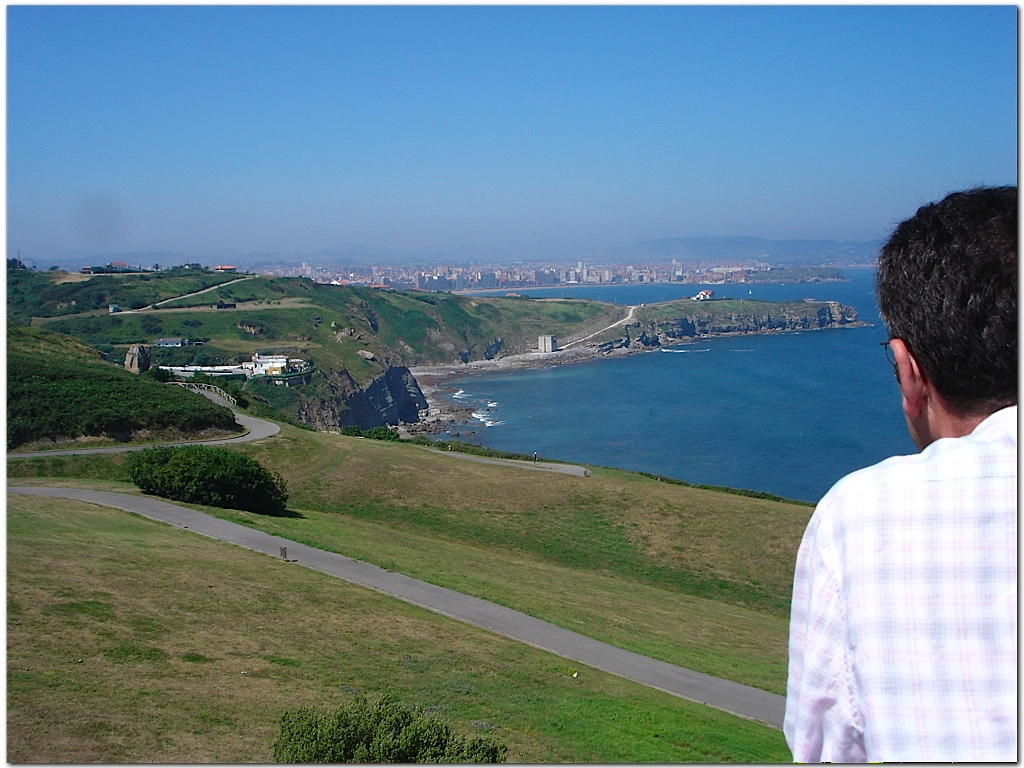
\includegraphics[width=300px]{images/Espana-805.JPG}\\
\textsc{Mirador Este de Gij\'on.} \end{center}

Bajando un poco por la costanera una escultura: ``la madre del emigrante''. Es
la primer escultura que me conmueve, lo llena a uno de esa desolaci\'on que el
artista habr\'a querido imprimir. Ver de este lado lo que estudiamos all\'a
como ``inmigraci\'on'' es simplemente esa imagen.

Esa tarde me met\'i en el mar. Terriblemente fr\'io al entrar, muy relajador
al salir. Y estar, un placer, desde que uno se acostumbra a las algas. Azul,
con pocas y suaves olas, y sin bancos de arena ni pozos, no tiraba ni para el
costado. Lo m\'as destacable es que en la escalera 7 (hay varias y bastante
unidas) estaba prohibido ba\~narse, y yo estaba en la 5. Las mareas y
correntadas cambian en pocos metros. El estar reci\'en llegado todav\'ia me
hac\'ia sentir el placer de meterme al mar en ``invierno''.

\begin{center}
  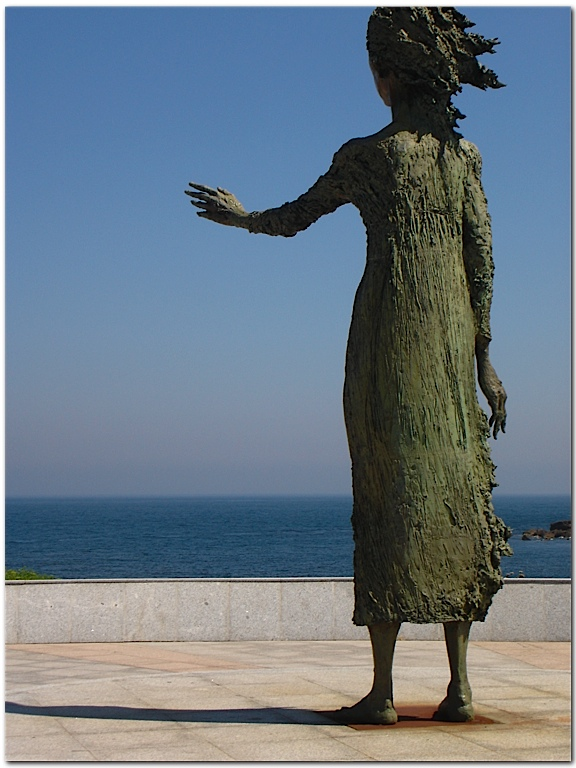
\includegraphics[width=200px]{images/Espana-812.JPG}\\
  \textsc{La madre del emigrante.}
\end{center}

En la tarde, la frutilla del postre: Covadonga. Un camino a los lagos que Uge
no recorr\'ia desde hac\'ia 30 a\~nos. Es \emph{perfecta} esa ruta, me dieron
ganas de comprarme una bici y recorrerla toda, y volver a Gij\'on por caminos
de tierra. De esos paisajes que se ven en postales suizas o austr\'iacas se
trata. Los terrenos, muy chicos, est\'an divididos por arbustos. Lo t\'ipico
de las postales de aqu\'i: una gran catedral con la imagen de la Virgen de
Covadonga, y un excelent\'isimo sagrario (en realidad lo repelo bastante, muy
tur\'istico y comercial me pareci\'o). Lo lindo de la catedral era verla inmersa
ah\'i, en ese bosque tan divino. Arriba de una sierra hay una imagen de Pelayo y
la cruz, donde seg\'un la leyenda ``casi'' se cae, y un camino que la un\'ia a
donde est\'abamos. \textexclamdown Me dieron buenas ganas de subir! Pero era
largo dice Uge. Despu\'es, la cueva donde apareci\'o la Virgen, hermosa la
imagen y la vista. Pero de nuevo lo mismo, yo estaba mala onda me parece por la
cantidad de cosas que se vend\'ia, y de gente curiosa como yo. Y de ah\'i, al
para\'iso.

Una ruta casi de una mano subiendo sin parar, escoltada por mucha vegetaci\'on
\emph{verde}, a veces tipo t\'unel; algunos ciclistas subiendo (en pocas horas
ser\'ian los m\'as felices del mundo con la cantidad de curvas que hay),
vaquitas en medio de la ruta con cencerros, y algunas ovejas de pelaje largo.
Primer mirador: desde muy alto a los valles verdes, a la ahora lejana catedral,
y atr\'as, los picos nevados. \textexclamdown Nieve! La ruta se ve\'ia por
cualquier ventanilla del auto serpenteando a trav\'es del bosque. Seguimos hasta
encontrar un auto parado: el conductor intentaba espantar a las vacas sueltas.
Miles que est\'an buscando sombra caminan por estas monta\~nas, parte de los
``Picos de Europa''. Salimos temprano para no encontrar demasiada gente, y dio
resultado.

Primer lago, y tras un cerro el segundo lago. Paramos, caminamos hasta el
cerro y se pod\'ia ver los dos lagos, adem\'as de diversos caminos para seguir
a pie. Paradis\'iaco.

Bajamos y cruzamos los tradicionales horrios, construcciones de madera
levantadas del suelo para guarecer a las vacas del sol, y guardar granos
alejado de las ratas. Conoc\'i el puente de Covadonga, lo conozco de
memoria por fotos y, a diferencia de lo que cre\'ia, est\'a en una ciudad;
pero verlo ``en serio'' fue maravilloso. Es como todos los castillos, uno sabe
que son as\'i, pero estar se siente diferente. Esta zona me enamor\'o.

Volvimos por la ruta ``vieja'' para parar en un museo de sidra (interesante,
lo m\'as: las prensas que usaban hace doscientos a\~nos, de madera y con
palancas, a m\'as larga mejor); y para disfrutar de las incontables curvas, que
si uno se cerraba demasiado choca con la sierra, y si se abre, contra el
guarda riel. Y Uge maneja muy bien as\'i que no se nos dificult\'o disfrutar
de esto \'ultimo. Vimos Gij\'on desde el d\'ecimo mirador (a cu\'al m\'as
hermoso), y vuelta a casa.

Me preguntan qu\'e como, y como como como en casa (\textexclamdown qu\'e
trabalenguas!) S\'olo que usan otras especias, pero todo muy producido y rico.
Nunca de m\'as ni tampoco de menos, bien medido. Si estaba rico y somos
glotones, \textexclamdown s\'olo entonces nos quedamos cortos! Pero
relativamente. Buena costumbre a la que no acostumbramos.

Y ahora ver\'e si el calor me permite correr como espero. Sino, al mar.
\textexclamdown Hay tantos problemas por los que preocuparse, en esta zona! Lo
comparaba con el viaje de 5$^\circ$ a\~no en ese sentido. Fuera de broma, hoy es
tapa del diario la sombra de un tibur\'on que apareci\'o en las playas, pero
dicen que no hace nada. Ya les contar\'e. O tal vez no\ldots En fin,
\textexclamdown de cualquier modo, saldr\'e a conocer!

\subsection*{Mi\'ercoles 13 de Julio}

Es impresionante c\'omo escribo pensando que pasaron varios d\'ias, pero son a
lo sumo dos.

La tarde despu\'es de Covadonga sal\'i a correr por la costanera hasta el
mirador del Este, que me hab\'ia encantado. Hab\'ia ido en auto y me enga\~n\'o:
la costanera est\'a \emph{llena} de subidas y bajadas. Pensaba ir y volver sin
parar pero, fulminado, me tir\'e en el mirador a contemplar las maravillas de
este infierno. Estaba ventoso. Volv\'i trotando, me tir\'e en el mar vestido
como estaba, y, ya en casa, me d\'i una \emph{gran} ducha. Luego una siesta de
20 a 22hs antes de cenar (fulminado, en serio), \textexclamdown y a la Semana
Negra!

La Semana Negra es una gran feria anual en Gij\'on, que tiene cosas tan variadas
e inconexas que da risa el s\'olo mirar. Los puestos son tipo la Rural de
Pergamino, pero el tema, nada que ver. Empez\'o como un encuentro sobre libros y
pelis de novela negra, pero termin\'o siendo una semana de fiesta, sin otra
excusa que las ganas de juntarse a tomar algo. El olor a frito mata. Hoy me
contaron que ayer estuvo Sabina y me quise cortar las venas. El mi\'ercoles
escuch\'e ah\'i a una banda h\'ungara (cientos de instrumentos de viento y un
ritmo muy movido) que me hizo recordar a Goran Bregovic. Todos puteaban porque
ni hablar se pod\'ia, pero al recordar el teatro y ser algo tan particular me
encant\'o. Tambi\'en escuchamos rockabily, es para mi jazz, pero, para el que
sabe del tema, mezclado con Rock \& Roll.

Muy bueno y divertido.

\subsection*{Jueves 14 de Julio}

Esta ma\~nana visitamos Cudillero. Otro pueblo antiguo y netamente pesquero,
pero colgado de la monta\~na, que cae abruptamente al mar. No hay calles,
subir hasta el mirador no es tarea sencilla. Cuando encontramos una, subimos
lo que ser\'ian dos cuadras para una ciudad planificada (pero sin bocacalles),
y una curva nos hizo hacer una ``V'' corta, como en los montes de Valpara\'iso.
Un hombre nos indic\'o que el mirador estaba ``despu\'es de la casa verde''. Sin
cruces de calle: hab\'ia que seguir el camino hasta encontrarla. Un laberinto de
casas antiguas, que se asientan como en gradas mirando al mar. Hab\'iamos
caminado un mont\'on por ser ``una cuadra'' pero \emph{nada} para estar
\emph{tan} altos. Es que todo es subida por calles estrechas, y mirando el
camino uno no nota cu\'anto avanza. \textquestiondown C\'omo har\'an los que
viven arriba para moverse, al envejecer? Varios gatitos de por medio, un poco
amigable pequin\'es, y dos viejitas charlando, nos indicaban que, m\'as que
caminos, \'estos son los patios de las casas.

Cuando llegamos se ve\'ia la grandeza del paisaje, sin interrupciones de tejados
o cables. \textexclamdown Y ni siquiera desde ah\'i arriba se ve\'ian caminitos
por la ciudad! \textexclamdown Son muchas las casas para que no est\'en
claramente unidas! Pocas para vivir en un lugar alejado, s\'olo alimentado
gracias al inmenso mar. Se ve\'ian barquitos pescando y un poco de trigo
salvaje, las piedras bajo el mar\ldots\ calculo que las fotos parecer\'an de
fot\'ografo, aunque el clima un poco nuboso y h\'umedo no era el propicio.

Bajamos del mirador caminando por otro sendero. Circul\'abamos casi a la misma
altura que un techo cuando vi sobre su chimenea a una gaviota del tama\~no de un
pavo real. \textexclamdown Hermosa! El plumaje suave me hac\'ia acordar al gato,
el cuerpo grande al de los gansos, la carita a \'aguilas creo, con el pico
curvado hacia abajo y los ojos tambi\'en grandes. Perd\'on si me pongo
t\'ecnico, es que la anatom\'ia animal es mi fuerte. Distingu\'i entre las tejas
a un bicharraco todo gris y desplumado, camuflado entre los colores de barro de
las tejas del techo; el hijo de la gaviota seg\'un Uge. Se ve que esta gaviota
enga\~n\'o a su gavioto porque ten\'ia poco de este animal el bicho, por ah\'i
al crecer se le aclara el plumaje. Le tomaba una foto cuando el pavo real se
hech\'o a volar y nos empez\'o a atacar. S\'i, ser\'ia el hijo este ave gris, y
la madre lo estar\'ia protegiendo sino salud\'andonos a modo ``gaviota''. El
tama\~no era, como ya dije, de dos pavos reales juntos. Hermosos bichos.

Pasado el peligro continuamos camino abajo, siguiendo una escalera antig\'ua y
de piedra que ten\'ia escalones para un costado, para el otro, con pocitos y
pasto, para adelante, para atr\'as\ldots\ Nada de horizontales. Hay que bajar
paso por paso, examinando c\'omo ser\'a el escal\'on que sigue, para llegar
hasta abajo sano y salvo.

Llegamos a una galer\'ia llena de sombrillas, donde se puede comer mariscos en
los numerosos restaurants. Sobre el turismo, no entiendo c\'omo hab\'ia tantos
autos en el estacionamiento, pero tan pocos turistas husmeando por el pueblo.

Al ver que era temprano (\textexclamdown c\'omo madrugo!), en lugar de volver
a casa Uge me llev\'o al barrio antiguo de Oviedo, la ciudad donde estudia
Jorge. Hermos\'isimas calles y edificios, peatonales y plazas, variedad de
esculturas en lugares p\'ublicos. Muy lindo, muy art\'istico. Breve recorrida, y
volvimos.

Esa tarde para todo argentino almorzamos pescados, tipo sardinas pero m\'as
grandecitos. \emph{Muy} rico. Otro d\'ia comimos ``bonito'', excelente
tambi\'en. Qu\'e l\'astima que en Argentina no se coma pescado, entre lo sano
y rico que es. \textexclamdown S\'i, entiendo lo del olor en la cocina!

Despu\'es del almuerzo, olv\'idense de sentarse a estar de ocio: visitamos
el museo del minero. La gu\'ia nos explicaba c\'omo era la mina desde un hotel
cinco estrellas: ``la verdadera mina es como lo ven aqu\'i, pero diez veces
peor''. Todo el camino se trat\'o de eso. \emph{Incre\'ible}. Incre\'ible
porque de ese hotel cinco estrellas dos mujeres pidieron que las volvieran a
subir, y nosotros no est\'abamos nada c\'omodos en ese subsuelo (lejano de los
640 m de profundidad en que trabajan). Las condiciones en la mina siempre
fueron y ahora son (no tant\'isimo, solo tan) malas. S\'olo contar\'e un
detalle, lo dem\'as es verlo para impresionarse. Bajando un pasillito desde
donde escarban la monta\~na para extraer carb\'on (en vez de usar la escalera,
usando el camino que usar\'ian los mineros, pero pavimentado y sin barro) nada
estaba horizontal o vertical; y mientras ve\'ia a mi lado que por la escalera
bajaban los ``grandes'', parec\'ian recostados sobre la nada y no verticales
al piso. \textexclamdown Me marea pensarlo! Si me daban un vaso de agua seguro
volcaba al sostenerlo. Hab\'ia perdido el sentido de lo que era vertical, y al
bajar a las v\'ias no entend\'ia nada. Todo interesant\'isimo, creia que las
minas eran otro lugar de trabajo, como los dibujitos mostraban. Las relaciones
minero/empresario, se imaginan, fueron de lo m\'as tirantes.

Cuando sub\'i al museo de m\'aquinas antiguas (\textexclamdown lo mejor!), Uge
me apuraba en cada punto: ``ve esto, Tute; ve aquello''. \textexclamdown
Encima di dos vueltas porque, cegado por alguna, siempre se me pasaba la que
estaba a mis espaldas! Una reproducci\'on de la m\'aquina a vapor hecha muy
grande permit\'ia entender claramente su funcionamiento y usos en la mina. El
vapor se generaba desde el carb\'on de la misma monta\~na. Tambi\'en hab\'ia
mucho sobre p\'olvora, importante para cavar los t\'uneles.

Completaban la gran muestra maquetas de accidentes en la mina, c\'omo eran los
hospitales, y textos que explicaban la evoluci\'on a trav\'es del tiempo. Sobre
anest\'esicos, fue tristemente gracioso leer sobre un m\'edico que,
inyect\'andose coca\'ina en los nervios a modo de prueba, se volvi\'o adicto. El
pobre termin\'o dedicando su vida a tratar la adicci\'on m\'as que a descubrir
novedades sobre anestesias. Mientras le\'ia sobre adrenalina, Uge y Jorge
comparaban riendo mi expresi\'on con la que tendr\'ia ese m\'edico;
\textexclamdown la pasamos de diez ah\'i adentro!

Sigo: \textquestiondown Saben lo que es el ``Gris\'u''? Adem\'as del bolichazo
de Bariloche (que simula una mina), es el gas metano mezclado con el aire de
la mina, se forma al desprender el carb\'on y caus\'o muchas muertes. Morboso
para mi el cambio de sentido de la palabra.

Ma\~nana viajo a M\'alaga, al sur de Espa\~na. Qu\'e bueno volver a volar; no
lo esperaba pero cruzar las monta\~nas de Asturias en tren o colectivo demoro
tanto que se hace la hora de ir a Alemania. Y cruzando Espa\~na el paisaje, si
bien lindo, es m\'as mon\'otono.

En Alemania volver\'e a escribir, seguramente bastante los primeros d\'ias. Si
Gustavo me lleva a todos los lugares que planea, entonces \emph{todos} los
d\'ias. Da igual, tengo ansiedad de s\'olo llegar.

\subsection*{Mi\'ercoles 20 de Julio}

\textexclamdown Hola familia, y feliz d\'ia a los amigos!

Estuve m\'as desconectado ac\'a en M\'alaga. Llegu\'e el Domingo a la noche
despu\'es de un excelente vuelo de casi una hora. Era un avioncito de dos
turbinas, chiquito, \textexclamdown pero tan (in)c\'omodo como el grande que
me llev\'o al otro lado del oc\'eano! Hasta que nos taparon las bajas nubes
asturianas pude ver la costa cant\'abrica, con sierras, quebradas y esas
peque\~nas finquitas; todo muy lindo. Despu\'es de una densa capa de nubes
oscuras, el encandilante sol. Despu\'es, la sombra del avi\'on proyectada
sobre el algod\'on, m\'as que blanco. \textexclamdown Hac\'ia d\'ias no ve\'ia
sol!

Llegu\'e, y me recibieron los amigos: Mangacha, Richard y su hijo de mi edad:
Gussy. Mucho lujo por aqu\'i, dicen que es la provincia m\'as pobre pero es la
m\'as ostentosa de lo que conozco. Alrededor de los grandes yates del puerto
Ban\'us se estacionan Ferraris, cuando no son las ``t\'ipicas'' 360 son las
m\'as grandes. Porsche Cayenne y Boxster, moneda corriente; 911 como
Volkswagen Boras all\'a, no tanto pero est\'an. Todos los autos son caritos, a
diferencia de Argentina, ac\'a un Audi A6 no llama la atenci\'on. Y tanto como
en el Norte, lleno de A8s. \textexclamdown Hasta vi un S8! Cuando me baj\'e
del avi\'on y no sab\'ia esto cre\'i que hab\'ia una muestra o algo porque vi
una Lamborghini, una Ferrari y una Cayenne juntas en un lugar. Pregunt\'e, y
me dijeron que as\'i es.

Menos verde y m\'as \'arido, me dediqu\'e a un tenis de una hora con Gussy y
padre, y a bicicletear por las sierras, que poco tiempo pero con los
desniveles y este \emph{sol} era suficiente para querer incendiar remera y
gorra al llegar. Vi un mont\'on de construcciones.

Comimos mejillones y dem\'as cosas ricas y aut\'octonas. Las paellas tienen
otro sabor. \textquestiondown Me estar\'e desquitando por los tallarines
caseros de ``la abuela'' que describen? Mangacha y flia divinos, sin ellos me
pegaba el embole del siglo. No paramos de pasarla bien. Le\'i bastante
tambi\'en.

Ma\~nana viajo a Madrid, noche en lo de V\'ictor y Mar\'ia, \textexclamdown y
pasado a Frankfurt! Donde tomo un tren a G\"ottingen.

Me voy de Espa\~na con algunas ense\~nanzas:

\begin{enumerate}
  \item{Groucho \emph{no} es Karl Marx. Ya vi dos pelis y hoy veo la tercera,
  \textexclamdown es un \'idolo!}
  \item{\textexclamdown El agua ac\'a gira para el otro lado en inodoros y
  piletas! Los Simpsons no mienten, el Ing. Civil Richard me explic\'o
  porqu\'e. De todos modos lo voy a filmar para ``cre\'ermela''. Estos no me
  enga\~nan.}
  \item{La manzana en las ensaladas queda bien.}
\end{enumerate}

Y otras cosas igual de brutas/interesantes.

Que pasen un buen d\'ia del amigo;

Tute.

\subsection*{Jueves 21 de Julio}

En M\'alaga no recorr\'i mucho pero tampoco estuve mucho tiempo. Para lo que
estuve hice lo justo: andar en bici por sierras, meterme en una linda playa
(llena de algas que me atrapaban y desesperaban) y conocer un poco la ciudad.

Llegu\'e a Madrid, y tom\'e el metro (subte) a lo de V\'ictor y Mar\'ia para
pasar la noche. Ac\'a los subtes describen c\'irculos por toda la ciudad,
hay 13 l\'ineas interconectadas y siguen construyendo. No transpir\'e tanto
como el verano urbano ameritaba, porque los vagones tienen aire acondicionado.
Desarrollo.

Divinos como siempre los anfitriones. Descans\'e y me ba\~n\'e, luego V\'ictor
cocin\'o una buena tortilla. Mientras la com\'iamos me contaba que ellos no
cenaban hoy, pero cocin\'o y cena para acompa\~narme. Charlamos de buenos
vinos, buenos jamones, buenos puros, buena carne\ldots\ \ \textexclamdown
Qu\'e lindo cuando la gente es fan\'atica y disfruta de las cosas! Si ven los
jamones que hay ac\'a se desmayan. Los cortan directamente de la pata, secada
en sal. Sabros\'isimos.

Me despert\'o V\'ictor, hizo el desayuno y me llev\'o al aeropuerto; no me
dej\'o ir en Metro. Malcrianza total. Me sent\'e al lado de la pista de
aterrizaje para esperar, y se ve\'ia todo el movimiento. Uno por minuto
calcul\'e. La de despegue ser\'ia del otro lado. \textexclamdown No lo pod\'ia
creer, tan seguidos! Verlos bajar me recordaba a los avioncitos de telgopor que
venden en las playas marpalatenses: uno m\'as arriba y atr\'as que el otro.
\textquestiondown Se acuerdan, todos atados? Ac\'a similar, pero sin hilos y con
turbinas que despiertan la curiosidad. Se ve\'ia hilera de a tres: el que tocaba
pista, el de atr\'as, y el de m\'as atr\'as.

No veo la hora de conocer Alemania.

\section{Pa\'is nuevo, vida nueva. Alemania.}
\subsection*{Viernes, 22 de Julio}

En este d'ia un poco nublado, me toc'o un avi'on c'omodo a Frankfurt.
\textexclamdown Qu'e emoci'on, por fin llegar a Alemania! Ir'iamos a Suiza para
despu'es virar al Norte y meternos en Alemania, es decir que no fuimos en
diagonal, y que vi cadenas monta\~nosas varias. Me sorprend'i volando a M'alaga
de ver un avi'on a lo lejos mientras nosotros 'ibamos en la misma direcci'on, en
comparaci'on esta ruta parec'ia una autopista: \textexclamdown cont'e 7 aviones
cercanos a nuestro vuelo! En uno me asust'e bastante: iba mirando alg'un lago
distra'ido, y pas'o \emph{\textexclamdown a fondo!} otro avi'on en sentido
contrario, poquito m'as abajo que nosotros. Se ve'ia grande y evidenciaba lo
r'apido que van estas m'aquinas, al pasar tan cercano. Uno ni se imagina la
velocidad, porque son m'as suaves que sentarse en un puf estos monstruos. Otro
se acercaba de costado y descend'ia para pasarnos por abajo. \textexclamdown Son
\emph{tan} grandes! Es muy tonto (mejor tildarlo de curioso) preguntarse esto,
pero me parece incre'ible el funcionamiento de los aviones. Es magia. Pasamos
monta\~nas, ciudades y lagos hermosos, un sue\~no, y vi un pico nevado sobre las
nubes bajas. Tambi'en se notaban varias pistas de aterrizaje desde el aire.

Bajando en Alemania se ve'ia todo perfectito. Los arbolitos, miles, todos en
fila india; las casas con techos a dos aguas, todas similares y de colores
ocres, marrones y amarillos; puentes y autopistas, trenes por todos lados,
barcos de carga en un gran r'io, este avi'on bajando, en fila con otros a este
gran aeropuerto. Todos {\small BMW}s (muchos ``rurales'', que all'a casi no
hay), Audis, {\small VW}, Mercedes, no muchos Porsches; todo prolijo, todo bien
hecho, todo lindo. No hay cosas que desentonen. Maquetas.

\emph{Toda} Alemania es verde, tupida. Voy a correr a un bosque cercano a la
casa, el camino es un t'unel de vegetaci'on por el que se filtran rayos de sol.
Lleno de subidas y bajadas que lo hacen m'as especial. Olv'idense de un camino
de 2~km sin curvas, eso no existe. S'olo en autopistas. Tengo bici para recorrer
las sendas, donde hay turbinas e'olicas. Parecen comentarios desprendidos, pero
sigue todo una misma l'inea: belleza y prolijidad por donde se mire y ande.
\textexclamdown Hasta el asfalto es m'as lindo! Yo no se porqu'e pero me gusta
m'as oscuro, y en Espa\~na era m'as claro. \textexclamdown Aunque si era al
rev'es seguro me gustaba el claro!

Al aterrizar tom'e primero un colectivo que me lleve a la parte 1 del aeropuerto
de Frankfurt, que es enorme. Compr'e un boleto de tren en esta zona 1,
\textexclamdown pero ni idea ten'ia d'onde tomarlo! Preguntando por aqu'i y
por all'a y caminando, llegu'e a un anden 1, pero subterr'aneo. Sub'i al tren
equivocado, obvio; lo tom'e antes por ansioso. \textexclamdown Pero le mostr'e
mi boleto a un alem'an puto y a las apuradas me dijo que era ese! Cuando no
ve'ia nunca la luz del d'ia y ve'ia que el nivel no se condec'ia con lo pagado
--y que paraba cada 100m-- me di cuenta de que no ser'ia\ldots\ pregunt'e, y la
se\~nora que se sentaba a mi lado me dijo que tome el subte (\textexclamdown en
un subte, no tren, estaba!) de vuelta, 4 paradas, y en ``Frankfurt Main'' mire
cu'al era mi tren; es decir que lo tomaba m'as adelante del aeropuerto y este
subte s'olo me llevaba a la estaci'on principal, \emph{Hauptbahnhof}. Menos mal
que pequ'e por temprano y no por tarde.

Llegu'e a la estaci'on y era m'as grande que el aeropuerto. Tenia \emph{seis}
minutos para la salida de mi tren desde all'i. Informaci'on estaba dos niveles
arriba. Sub'i corriendo por las escaleras con mochila y bolso, todav'ia me
pregunto c'omo llegu'e sin dejar las rodillas por el camino. Si tomaba las
escaleras mec'anicas la gente me demoraba, \textquestiondown y a qui'en se le va
a ocurrir usar las fijas? Al preguntar en Informaci'on, col'andome con permiso
y cara de ``llego tarde, \emph{\textexclamdown enschuldigung!}'', me quedaban 4
minutos pero era cerca: and'en 7.

Pregunt'e a una joven pareja ah'i mismo para confirmar, y contestaron que sale
del and'en 6.

\subparagraph{}\label{ssub:AngeldelaGuarda} --- \textexclamdown Pero en
informaci'on me dijeron 7!\\ --- Pero lo cambiaron a 'ultima hora.\\
\hangindent=1cm

Y les cre'i, porque ellos tomaban el mismo tren: pasaban G\"ottingen. Si nos
equivoc'abamos, nos equivoc'abamos juntos, y m'as vale eso que no estar seguro
solo. Una hora de viaje por valles, sierras, campos y fincas, parado en un tren
m'as suave que el avi'on; y despu'es de saludar a la pareja 'angel-de-la-guarda
cari\~nosamente, baj'e en mi nueva ciudad.

Taxi a la joyer'ia de Gustavo, y \emph{here I am}, por fin. De taxi un Skoda,
del nivel del Passat o mayor. Todos {\small TD}is. Yo no lo puedo creer.

Me instal'e, bien recibido por toda la familia (Gustavo e Ina, y sus hijos,
Pablo y Felipe). A cenar y descansar.

\subsection*{S'abado, 23 de Julio}

Hoy conoc'i a un amigo de Gustavo, ``Folka'', de unos 65 a\~nos. ``Folka'' es
una parte de su nombre, que empieza con ``\emph{Volks}''; significa hombre del
pueblo (y no, no existe el femenino de ese nombre). Sabe 5 idiomas
perfectamente, y me dej'o picando la posibilidad de visitar Turqu'ia en Agosto,
en un ``viaje de cultura''. Simp'atico el tipo, adem'as. Profesor de universidad
de idiomas y geograf'ia. Conduce un New Beetle negro descapotable. Viaj'o por
todo el mundo, a Gustavo y a mi nos ense\~na castellano y sobre cosas que hay en
Argentina, Chile, Per'u\ldots\ Y lo hace con buena onda, sin arrogancia. Juega
al tenis y lo lleva loco a Gustavo: ``todas a los pies''.

Al abuelo de Ina lo mataron en la II Guerra Mundial. No lo llevaron al frente de
batalla porque con su auto --uno de los pocos-- tra'ia v'iveres a la ciudad.
Pero alg'un nazi o cobarde denunci'o algo y lo llevaron a fusilar. Claro que es
la historia que ellos me cuentan no la del denunciante, pero es perfectamente
posible. Estoy leyendo ``Stalingrad''. Cada d'ia que pasa veo lo irracional que
son las guerras. Y cada p'agina del libro tambi'en me lo muestra.

Vi partes de la divisi'on Alemania comunista/federal. Me atosigaron con charlas
pol'iticas al verlo. Debe haber sido interesante, pero al no estar bien
instruido y le'ido no pude aprovechar la discusi'on.

Ayer a las 5pm est'abamos asando en la parrilla nueva de Gustavo. No sab'iamos
si almorzar o cenar (ac'a se almuerza tipo 3). Cre'imos que merendar'iamos pero
la sobremesa hasta las 8 nos indic'o que se trataba de una cena. Les ense\~n'e a
hacer matambre al lim'on. Como no existe el matambre Gustavo fue a la
carnicer'ia y le indic'o al comerciante que sacara una vaca para mostrarle qu'e
cortar.

Hoy comimos en un pueblo afuera de G\"ottingen, un restaurant ``t'ipicamente
alem'an'' seg'un Ina; delicioso todo. La cerveza ac'a me gust'o. No es helada.
No es tan amarga.

Volvimos por una ruta que pasaba cerquita de las turbinas e'olicas,
\textexclamdown su enormidad espanta! Despu'es vimos decenas de ovejitas,
dos perros, y un pastor. Era un encuentro de pastores, todos vestidos muy de
'epoca me pareci'o. Hab'ia cientos de autos, cientos de personas, y dos
chiringuitos vendiendo helados y cervezas. Me pareci'o un poco americana la idea
porque estaban todos en las mesas charlando y riendo, sin dar ni bolilla al
pobre pastor arreando las muchas ovejas. Eran la excusa para juntarse a tomar en
un prado. Los dos ovejeros alemanes corr'ian y ladraban, y el pastor con su
bast'on llevaba a todas las ovejas por donde quer'ia. Otro pastor ten'ia un
bast'on muy raro. Al preguntarle de qu'e se trataba, despleg'o dos palitos
formando una silla de cuero, y enterrando una punta se sent'o c'omodamente y
cruzado de brazos ante nosotros. \textexclamdown Pago en d'olares esa sillita
para mis viajes! C'omodo y divertido artilugio.

El BMW serie 5 de Gustavo pierde parte del encanto al enterarse uno de como lo
adquiri'o. Una mujer se lo cambi'o junto a muchos euros por un anillo y un
reloj. Es decir que esa \emph{m'aquina} vale lo que para una mujer dos joyas.
Que las personas somos diferentes no hay dudas. \textexclamdown S'olo Dios nos
puede llegar a ver iguales!

Aqu'i \emph{todas} las bicis llevan luces a d'inamo, que se dejan en las calles
porque no existe el robo, al menos en G\"ottingen. Y cada beb'e de cada edad usa
la sillita correspondiente para el auto, por seguridad ante posibles accidentes.
Aunque a veces, con tantos cuidados, se pasan del equilibrio me parece (no es
este el ejemplo).

Todos me dec'ian que es un lugar muy diferente Alemania, y no se equivocaban. Me
encanta.

\subsection*{Domingo, 24 de Julio}

Conoc'i hoy a tres parejas amigas de Gustavo: dos alemanas que no hablaban otro
idioma, y otra alemana que hablaba ingl'es, y el hombre es un fan'atico de todos
los deportes. Practic'o casi todos en serio, hasta esos saltos atl'eticos de
todo tipo que no conozco el nombre. Tiene una hija pre-adolescente m'as
vergonzosa que una paloma pergaminense, que quiere que aprenda castellano.
Porque ya habla alem'an e ingl'es (con 13 a\~nos) pero quiere que aprenda
espa\~nol para cumplir con facilidad los dos idiomas extranjeros obligatorios
que le exige la escuela secundaria. Ya hizo un viaje de intercambio estudiantil
a Estados Unidos que le gust'o. La otra opci'on era franc'es pero concluyeron
que no lo usar'ian tanto como al espa\~nol. Me comprar'ia, por ejemplo, boletos
en tren a \emph{Hannover} para conocer el zool'ogico y todo lo que tengo que
hacer es lograr que mantenga conversaciones en este idioma. Un poco ya sabe, no
ser'a imposible como cre'ia. Me pidi'o dos meses, todos los d'ias. Al terminar,
si todo anduvo bien, pagar'ia adem'as un viaje a Egipto para bucear en el mar
rojo (antes de Octubre).

\textexclamdown Viajar'ia a Egipto a bucear! Todav'ia Gustavo dice ``hay que
arreglar para que conozcas las pir'amides, todo''. Hay tiburones y ``\emph{all
kind of color fishes}''. Me ense\~nar'an buceo, mientras, en una pileta de
G\"ottingen. Ellos saben que yo vine a conocer cosas nuevas. Lo grande es que no
me dicen c'omo, \textexclamdown sino que adem'as me invitan!

Me contaba este hombre, Axel Becker, que viaja a Austria 2 semanas. Entonces me
deja su buena bicicleta todo terreno para andar por los bosques G\"ottingeanos,
mucho mas c'omoda y divertida que la de paseo que me presta Gustavo. Al final no
creo que la use mucho porque\ldots\ \textexclamdown me invit'o a pasar con su
familia y otra amiga a Austria! \textquestiondown Qu'e har'iamos en Austria dos
familias alemanas y un argentino? \textquestiondown Cu'al es el inter'es que los
une en un viaje? ``\emph{Wild Life} europea''. 8~km de un camino de piedras,
cerrado por una tranquera austr'iaca, hasta una casa sin electricidad ni
comodidades t'ipicas. Hay que buscar agua de vertiente, y bajar todos los d'ias
a un pueblo en bici a comprar el pan. Buena onda la familia, Gustavo asegura. 7
horas en una ``Touran'' (la van de camping de Volkswagen) hasta Austria. Hay
nieve, osos pardos (no los veremos seg'un dicen, espero Dios no los oiga),
ciervos (bambis), 2 vaquitas cerca de la casa, y otros bichos que ya no me
acuerdo. La casa es de un conde que tiene un palacio y grandes terrenos. Los
primeros tres d'ias los pasamos en el palacio como para compensar la falta de
comodidades de las otras dos semanas, que pretend'ian ellos asustarme pero son
las que me llaman a ir. Todos estos son proyectos, se llega a concretar alguno y
soy el hombre m'as feliz del mundo. Todo verde dicen, hay caballos, bicis y cada
uno se lleva sus piernas para recorrer. Espero que tambi'en algo para
protegernos, porque otro de los bichos eran ``\emph{wild pigs}'', jabal'ies.
Dicen que no son peligrosos, pero de eso no me f'io tanto. \textexclamdown Ya
les contar'e! Dicen que la sidra preparada por estos campesinos es riqu'isima.
Sino, la tendr'e que tomar igual porque hay pocas opciones, pero todo ser'a
casero.

En este encuentro sali'o un viaje a Egipto, otro a Austria, y curso de buceo;
sin mencionar que el asado argentino se celebr'o en Alemania. Turqu'ia, como ya
dije, era muy loco y voy ``invitado'', no invitado. Entonces no me alcanza el
dinero, o s'i pero para nada m'as. Esto es ``\emph{all inclusive}''.
\textexclamdown De todos modos mucho no voy a gastar en Austria porque no hay
donde usar plata! Ma\~nana voy a trabajar a la agencia de viajes del loco (solo
de viajes de buceo, vean qu'e especificidad) para terminar un sitio web de
Argentina antes de desenchufarme del mundo. Las compus de Gustavo son malas
excepto la mejor del mundo, que est'a en la vidriera de la joyer'ia por poco y
no la puedo usar. Desenchufarme en Europa me suena contradictorio.

Cuando Gustavo me lo present'o, dijo: ``se llama Axel, como Blumberg''. Sigue
las noticias argentinas el loco.

Una de las primeras cosas que le cont'e fueron mis viajes y proyectos de viaje
en bici (qu'e iron'ia, con proyectos ac'a). Esto ya parece medio loco tambi'en,
pero me dijo que podr'ia trabajar en su agencia para integrar cicloturismo (y no
trabajar solo buceo). Con contarles mis viajes, ense\~narles cosas, armar un
posible viaje de los que ya hice estar'ia adentro. Dios quiera que salga,
\textquestiondown se imaginan qu'e placer m'as grande ganar \geneuronarrow{1}
por contar mis viajes o proyectar? \textexclamdown Si fuera lucrativo vivir'ia
de eso en Argentina! Adem'as necesito actividades en esta vida ac'a. Aunque si
salen todas, de verdad no me alcanzar'a el tiempo. Una de las parejas alemanas
eran capas en la universidad y ver'an la posibilidad de ir a estudiar el idioma,
4 horas todas las ma\~nanas. Muy bueno, interesante.

\subsection*{Lunes, 25 de Julio}

Hoy a la ma\~nana pase'e en bici por G\"ottingen. Me dieron ganas de sacarle una
foto a'erea al cruce principal. Hay bici sendas por muchos lugares, y este cruce
es una obra de arte. L'ineas blancas por todo el asfalto, veredas con colores en
el piso para separar peatones de ciclistas, y dos sem'aforos de cada lado:
peatones y bicis, y autos. Ac'a se usa mucho la bicicleta, y es hermos'isimo
verlo. Si vieran qu'e nudo mas complejo parece, y c'omo organiza r'apida y casi
m'agicamente a este enjambre de veh'iculos entender'ian lo perfectito que se ve
todo. Es como las im'agenes de ciudades que repart'ia el ``Billiken'', todo
perfectito. \textquestiondown O ser'a que estoy de vacaciones? No se ven esas
cosas comunmente all'a, porque no hay bicis, de las que hay no son respetadas
como medio de transporte alternativo. Y 'estas tampoco respetan al no ser vistas
de noche, o por no tener patentes que identifiquen. \textquestiondown El huevo o
la gallina?

Despu'es dorm'i una peque\~na siesta porque llov'ia, y al despertar estaba
soleado. Sal'i a correr al bosque, antes de que se vuelva a largar (a la noche
lo hizo). Corr'i bien creo, pero las subidas y bajadas no me permiten comparar
con lo que hago en Argentina. Bajando trabajan las rodillas, y subiendo el
coraz'on, que me pide m'as aire que el que hay en todos los bosques. Pero
justamente estos accidentes geogr'aficos hacen que quiera llegar ``hasta la otra
curva y nada m'as'', para ver qu'e hay del otro lado y se repite en cada curva.
Y siempre encuentro lo que esperaba: belleza natural. Despu'es de la lluvia
hab'ia un olor a tierra mojada que parec'ia energ'ia para correr. Aire
\emph{fresco}. Los caminos son anchos, pero se puede tomar los internos que se
meten entre los 'arboles y tienen el ancho de una bici.

Reci'en comimos un terrible asado. Les gust'o la idea del lim'on en el
\emph{killhungry} (``matambre'', ac'a la traducci'on se hace directa).
Ensaladas de todo tipo, tienen tantas cosas raras que no puedo creer que sean
ricas. La mesa era un desorden: tres idiomas hablaba Gustavo y yo trataba de
seguir mi ingl'es. No s'e como las otras dos parejas alemanas no se enojaron:
casi nunca se integr'o en ese idioma. Simp'aticos todos.

Axel me contaba (sobre el tema que siempre llamar'a mi atenci'on) que despu'es
de la Segunda Guerra Mundial sigue el {\small NPD} y grupos neonazi. No los
pueden censurar por la Constituci'on, pero a diferencia de lo que yo pensaba son
menos del 5\% del pa'is. Le dije que me parec'ia una locura de gente, pero
contest'o que siempre hay locos para todo, y que ``mientras sean poquitos los
podemos contener''. Todos los alemanes (dec'ian 'el y Gustavo), son dem'ocratas,
o republicanos, o lo que sea el {\small SPD} que es el que ahora gobierna.

\subsection*{Martes, 26 de Julio}

En estos barrios el mundo parece perfectito en serio, y chocan los mails del
diario por eso. Claro, es que \emph{este} mundo se acerca a lo que llamo
``perfectito''.

A la ma\~nana fui a las oficinas a hacer unas cositas. Axel me invit'o a
almorzar y despu'es unas gu'ias tur'isticas de la agencia me mostraron un poco
G\"ottingen. Me mostraron una edificaci'on del a\~no 1412. Y varias casas tan
vencidas que dan ganas de quedarse haciendo fuerza para evitar el derrumbe.
Pasamos por un restaurante ``espa\~nol''. Todo lo que ten'ia de espa\~nol era el
men'u, porque la imagen era claramente norteamericana, con algunos indios
mejicanos.

Y a la tarde, \textexclamdown por fin cac'e la bici nueva! Es una m'aquina, m'as
c'omoda que la m'ia (el cuadro m'as grande la hace mas c'omoda, aunque menos
``canchera''), y con cambios m'as r'apidos y precisos (\textexclamdown a'un!).
Me emocion'e, y al llegar a casa cambi'e los pantalones y sal'i al bosque. Para
conocer m'as, en vez de doblar y volver a casa, segu'i el camino derecho.
Despu'es de cruzar todo el bosque llegu'e a las turbinas e'olicas. Me asustaba
un poquito primero por el t'unel del bosque, que hace que no se vea a un metro
de distancia, estando solo en un camino poco transitado. Despu'es, no se porqu'e
(como algunos a los payasos, sin raz'on aparente) pero de cerquita ver esas
turbinas girando tan despacito y tan inmensas, me daban un poco de respeto
tambi'en. No pod'ia pasarlas como por al lado de un poste, las vigilaba como un
perro al caballo. Es raro. Es lo mismo que siento cuando pasa un avi'on de esos
de publicidad mientras estoy dentro del mar en Mar del Plata, hay algo en eso
que me desespera.

Agrego para la ing. qu'imica de Espa\~na que las turbinas e'olicas son
\emph{muy} silenciosas. S'olo se escuchaba mi respiraci'on y los cultivos
mecidos por el viento. \textexclamdown A no andar usando razones inveros'imiles
para apoyar la energ'ia at'omica!

Llegu'e a un pueblito, donde tom'e un camino de campo. Las subidas y bajadas y
curvas entre trigo y girasol, y c'omo se ven los tejados a dos aguas de pueblos
lejanos entre las sierras, son de f'abula. Llegu'e a otro pueblo, y ya quer'ia
volver. En 6~km cruc'e tres pueblos, \textexclamdown igual que en los caminos de
Pergamino! Volver'ia por el mismo camino (imposible volver a encontrarlo
despu'es de tantas bifurcaciones, adem'as ya lo conoc'ia) o describiendo un
circuito. No anduve mucho, unas 2 horas, pero a la hora ya me empieza a
interesar saber donde estoy. Di una vuelta enorme, y describiendo una ``V''
corta volv'i a las mismas turbinas e'olicas, pero ahora ve'ia la ruta con
carteles a G\"ottingen. \textexclamdown Y los techos que vi en todo el camino
eran los de la ciudad que buscaba, que cre'i estaba del otro lado de los
bosques! Es decir que el camino por bosques est'a lleno de curvas que no cont'e,
y hace parecer mucho m'as largo un mismo recorrido. Ahora, a conocer siempre que
pueda, aprovechando los pocos d'ias de buena bici.

La bici tiene 8 pi\~nones, 24 cambios. En algunas bajadas los tiraba a todos y
iba realmente \emph{r'apido}. Al tocar los frenos se sent'ian tan suaves aunque
potentes, como una moto que pesa 10~kg. Ese es el placer de las bicis. En
las curvas cerradas en pavimento en bajada se escuchan los tacos de las
cubiertas todo terreno. \textexclamdown Y la vegetaci'on de los costados
magnifica la sensaci'on de velocidad! Gracias, Axel.

La pr'oxima espero volver a perderme, porque ac'a todo es cerca. Y saber que
est'as perdido, que parece que est'as lejos, pero que en media hora pod'es estar
de vuelta en casa se siente bien. Para dar una idea, lo que hice hoy es como
llegar a Arroyo Dulce desde Perga (sin la vuelta), pero cruzando 4 pueblos. Y
tres turbinas e'olicas: una grande y lenta, y dos m'as peque\~nas y r'apidas. Si
estoy perdido alguien me va a ubicar entre tantas peque\~nas poblaciones. Todo
el mundo habla ingl'es, y todos se excusan de que lo hablan ``\emph{a little
bit}''.

Ma\~nana me espera un d'ia similar, y con confirmaci'on de Austria.
\textexclamdown Qu'e aburrido, un d'ia similar!

\subsection*{Mi'ercoles, 27 de Julio}

El no parar de mover las piernas y el clima pesado me llevaron a quedarme en
casa, as'i que le'i, dorm'i, y anduve poco en bici por la ciudad. Les cuento que
en Austria ``el palacio tiene solo dos habitaciones armadas'', as'i que no puedo
ir. Triste, pero igual no era planeado. Axel me pregunt'o si quer'ia
``cambiarlo'' por Egipto. ``\textexclamdown Pero era un regalo!'', contest'e.
As'i que tengo dos semanas de bici sin parar. Despu'es saldr'e a correr,
mientras la aprovechar'e.

Hoy visitar'e alg'un bar G\"ottingense para ver qu'e onda. Aunque quienes me
llevan son aficionadas al hip-hop, calculo que en el bar un Mi'ercoles ser'a
m'as tranqui la onda. Son quienes trabajan en la agencia de viajes, la semana
que viene hacen el mismo viaje a Egipto. Tienen que viajar por trabajo, para
conocer el producto que venden. \textexclamdown Muy buen trabajo! Veremos
qu'e cuentan cuando vuelvan, la siguiente semana.

\subsection*{Jueves, 28 de Julio}

Hoy me levantaron no muy tarde para ir a Kassel, a un complejo tur'istico muy
grande de termas y cosas de relajaci'on. Menos mal que fuimos, porque sino, con
el estr'es que vengo acumulando muero. Fuimos la familia menos Ina, que trabaj'o
en la joyer'ia. Todo muy bueno: jacuzzis, todas las piles climatizadas y con
sales; me met'i en un sauna y todo. Est'a bueno porque hace transpirar todo el
cuerpo. Uno juega al tenis y transpira casi todo, pero en el sauna se transpira
el 100\% de la piel. Con ``aromaterapia'' que recordaba al living de casa. El
cartel dec'ia ``80 a 90 grados''. Parece que quemara al entrar pero no. O debo
ser \emph{re}bruto y lo deben medir en otro lado. Seguro. Solo al salir queman
los pies, que sino descansaban sobre la toalla. \textexclamdown Es divertido ver
a la gente salir corriendo!

El nudismo no es cosa del otro mundo. Entonces no se para qu'e se sacan todo,
seguro encuentran alguna raz'on que desconozco. Cuando es tan natural uno
ni se da cuenta, es casi lo mismo s'olo que se ven partes m'as blancas del
cuerpo. \textexclamdown Cuando me vaya de Alemania seguro el Gobierno me vuelve
a invitar para volver a embellecer Kassel!

En la pile de afuera se ve'ian aviones cada dos por tres, y los caminitos de
nube que van dejando, cruzados o paralelos. Se nota que Alemania es transitada
all'a arriba, un piloto ac'a debe tener poco tiempo para tomar mates.

Seguimos paseando por Kassel despu'es de las termas, y llegamos a un palacio.
Los chicos estaban muertos en el auto pero quer'ian bajar porque ve'ian a ``los
grandes'' hacerlo. Se ve'ia un camino todo verde que era pasto importado
de Inglaterra para m'i, que sub'ia un gran cerro (lleno de gente) hasta llegar a
un antiguo y gran castillo, lejaano lejano. Bajaban dos bicis de descenso (esas
que parecen moto-cross por forma, precio y velocidad), calculo que la sonrisa
no les entrar'ia en el casco a los ciclistas. \textexclamdown Qu'e diversi'on!
Andar as'i, por un lugar sin camino. Pero no lo visitamos hoy, porque los chicos
estaban inquietos.

En vez de volver por la autopista, lo hicimos por la ruta vieja. Paramos en un
pueblo muy antiguo, \emph{Hann-M\"unden}. Todas las casas son del siglo {\small
XV} o {\small XVI}, y la mayor'ia est'an vencidas; hay una capilla grande hecha
con piedras de todo tama\~no, otra iglesia m'as grandota con un techo alt'isimo
y un campanario original, un puente que cruzaba un r'io muy bonito lleno de
patos y ``una garza gris con pico rojo'' (el patito feo entre todos los patos).
Sobre este r'io se proyecta toda la vegetaci'on, y un palacete relativamente
moderno. Las mesas en la calle invitaban a un chocolate caliente. Gustavo sac'o
una foto a una fecha pintada en una casa: ``1657'', y no era la m'as vieja. Le
pregunt'e para qu'e, y era para comparar la historia de una antig\"ua
civilizaci'on, con la de Argentina, en una peli que est'a haciendo.

\textexclamdown Hasta las gr'uas de la construcci'on son menos feas por aqu'i!
No son en forma de ``T'' sino de ``L'' invertida, m'as bonitas, con tensores
diagonales. Los pesos van abajo, no arriba.

Seguimos viaje, y la ruta se torn'o tan angosta que cre'i que era de un sentido.
\textexclamdown No se c'omo se animaron unos ciclistas que adelantamos a
tomarla! El camino lleno de curvas no nos llevaba a G\"ottingen porque el
desv'io estaba cerrado por reparaciones. Preguntando llegamos a un ferry que nos
cruzar'ia por el r'io hacia otro desv'io. No se ve'ia motor: cruzaba con la
energ'ia de la correntada, sostenido por dos sogas a un cable transversal,
simpleza total. Ese debe estar bueno para que lo conduzcan las mujeres:
\textexclamdown solo puede chocar con dos riberas de pasto!

El ``be-eme'' serie 5 parece ser una m'aquina placentera en las rutas, pero
despacio no se nota, y fuerte no me animaba a disfrutarlo. Es un 6 cilindros y
ruge como un motor grande. Gustavo se quiere comprar un Laguna, \textexclamdown
pero comprar un importado en Alemania es una paradoja! Comprar importados all'a
en Argentina es comprar todos, pero entre lo ``grande'' es comprar alemanes
creo. Dice que dentro de Alemania la de m'as prestigio es Audi. Pero la verdad
es que los rurales {\small BMW} son m'as bellos. L'astima que no hay con
tracci'on integral.

Ahora tengo planeado irme con bici (se suben en el tren) a Kassel, separado por
unos 50~km, para recorrer bien todo lo que qued'o. La vista hacia abajo desde
all'a debe ser indescriptible.

Siguiendo con ``proyectos raros'', Gustavo est'a viendo la posibilidad de dar
una vuelta en globo aerost'atico. \textexclamdown Tiene cada amigo que me hace
morir de risa!

Es impresionante c'omo cambia el clima en un d'ia. Anoche hubo lluvia y tantos
rayos (sin sonido: ``que van de nube en nube'') que me daba cagazo dormir.
Duermo bajo un ventanal. Hoy, sol pleno. Y esta noche, \textexclamdown tormenta
m'as ventosa y ruidosa que la de ayer! As'i se mantienen los bosques verdes, y
el sol en la tarde para disfrutarlos. Sincronizaci'on perfecta hasta ahora.

\subsection*{Viernes, 29 de Julio}

Hoy fue incre'ible. Me levant'e temprano con tormenta. Toda la ma\~nana y
almuerzo: sol, las chicas en la agencia de turismo me preguntaban qu'e hacia de
pantal'on largo. Me acost'e media hora despu'es de almorzar, para salir luego a
andar en bici, pero ahora llov'ia. Una hora despu'es par'o, y no lo dud'e, las
nubes no amenazaban demasiado. Sal'i, esta vez con c'amara de fotos. Me
invitaron a una pile pero prefer'i pedalear por lugares nuevos, \textexclamdown
hice bien!

Tom'e otro camino, como estaba tan mojado no pude acelerar mucho en las bajadas.
En pocos minutos estaba en un cruce conocido, que cre'ia lejano. Es f'acil de
perderse en caminos boscosos. En media hora estaba en las mismas turbinas
e'olicas que antes de ayer hab'ia visto a la hora de pedalear. Y el mismo
pueblo, \emph{Diemarden}, poco m'as abajo. Estuvo bueno porque pedaleaba por ese
t'unel todo oscuro de vegetaci'on, que no se ve por donde sigue el camino, y
``redepente'' llegu'e a un claro, un cultivo de trigo. A mi derecha por el
camino acompa\~naban los bosques, y al terminar la cortina verde aparecieron de
golpe y cerquita las turbinas e'olicas y casi me da un espasmo. Por suerte a la
vuelta me amigu'e y me puse al lado para apreciar su tama\~no (estaban paradas).
Por los pueblos hice un mont'on de fotos que parecen postales, pero no por
m'erito del fot'ografo sino de la Naturaleza que rodea.

No me gustaba la idea de seguir por los mismos caminos pero hab'ia llegado sin
querer, as'i que tom'e otro desv'io, de esos que por ac'a abundan: un camino que
se abr'ia, todo poceado y viejo, oscuro por la vegetaci'on. Parec'ia que llevaba
a lo que llamamos all'a un casco (ac'a no existen las ``estancias'' calculo)
pero un cartel indicaba que a escasos 2~km hab'ia un pueblito. \textexclamdown
20 cuadras y otro poblado! Los 2~km fueron de subida, y arriba de la colina
esperaban dos grandes techos: eran establos y de eso se trata \emph{Bettenrode},
solo equitaci'on. Hermos'isimo. Cuando llegu'e les mostr'e las fotos a Gustavo e
Ina porque no lo conocen, \textexclamdown las ventajas de la bici! En Argentina
viajamos en bici para ver cada detalle, pero ac'a para ser tan detallistas
habr'ia que caminar.

Despu'es de mirar un poco esto, segu'i el cartel de bici senda que indicaba
un camino que parec'ia privado pero que era ``p'ublico'', entre comillas porque
parece muy poco usado. Lo segu'i para ver qu'e hab'ia, y despu'es de una curva
la encontr'e: la bajada de la colina. En todo el viaje se ol'ia la tierra
mojada; se tienen tantas sensaciones juntas, durante tanto tiempo. El tema de la
bajada es que tambi'en estaba cubierta por 'arboles y arbustos y por tanto muy
barrosa, llegu'e a abajo todo sucio. De nuevo me sorprendi'o el final de este
camino: bajando por aqu'i y por all'a, r'apido, oscuro en la vegetaci'on,
apareci'o un techito de esos t'ipicos alemanes, antiguos. Yo, creyendo que
estaba llegando a una casa s'uper antigua que no conoc'ia ni el due\~no,
aceler'e. Al llegar se acab'o todo el bosque y sent'ia de nuevo el sol. Era un
pueblo que estaba a\ldots\ \textexclamdown 10~km de G\"ottingen! \textexclamdown
Y yo pensaba estar el doble de lejos! Ah'i estaba la ruta, \textexclamdown es
que uno no se puede alejar, ac'a! Y sin embargo \emph{siempre} hay cosas nuevas.
El camino desembocaba en una capilla del 1730, alta sobre una gran roca.

Segu'i por la bici senda a otro pueblo que estaba a 1,6~km para el otro lado.
Pensar que en Pergamino hago 50~km para ver Fontezuela, la Olla y si tengo
suerte unos b'uhos, y por aqu'i cada 20 cuadras aparecen pueblos, bajadas,
subidas\ldots\ Este pueblo era puramente campesino. Lleno de establos, vacas,
se\~nores que usan jardineritos, tractores, y una capilla con un peque\~no
monumento a los ca'idos en las guerras mundiales. Para mi los libros para
ni\~nos se escriben ac'a.

Al volver al pueblo de la capilla alta en la roca, el cartel de bici senda
indicaba G\"ottingen a 21~km, aunque por la ruta se acortaba a 11~km. Obvio
quise tomar la bici senda, pero a los 5~km desemboc'o de nuevo en la ruta y no
la pude seguir. No s'e porque la perd'i. Es dif'icil querer volver a casa porque
siempre se quiere seguir ``un poquito'' m'as hasta el ``'ultimo'' pr'oximo
pueblo, que es siempre pen'ultimo. Al volver se abr'ian caminos desde la ruta
que llevaban a las turbinas e'olicas, paradas seguramente por poco viento.
Hab'ia autos abajo y pude comparar el tama\~no: inmensamente grande. Y eso que
'estas eran las ``chicas'', la ``grande'' era inmensa de verdad. Se usan
camiones completos para transportar s'olo las aspas (imaginen: el radio es del
largo de un cami'on con acoplado).

Llegu'e y com'i todo, como siempre. Chocho de haber encontrado esto. Seguir'e
conociendo estas semanas de bici buena. Cuando la devuelva empezar'e a viajar en
tren seguramente. \textexclamdown Podr'ia visitar varias terminales
automotrices! Y conocer la Selva Negra.

Ma\~nana voy a jugar tenis, dobles con Gustavo; contra Folka, y un tipo al que
le salv'o la vida Gustavo. Lo vio tendido en la calle con un paro card'iaco y le
empez'o a empujar fuerte en el pecho, luego le hizo respiraci'on, y ahora vive.
\textexclamdown Estaba muerto! Me dieron ganas de aprender eso, se debe dictar
en la Facultad de Medicina. Es reanimaci'on, en la escuela me lo ense\~naron
pero se imaginar'an c'omo me acuerdo. Cada vez reniego m'as de la bastante
precaria educaci'on en mi escuela. \textexclamdown Pero c'omo la agradec'i, de
estudiante!

\subsection*{Lunes, 1 de Agosto}

El s'abado fuimos a jugar al tenis. Nos alegr'o que Pergamino no viera a sus
representantes en este mini torneo porque nos limpiaron r'apido. \textexclamdown
Qu'e lindo tenis tengo! (No traje abuela, che.) L'astima que juego tan poco. La
misma excusa se le ocurri'o a Gustavo. Pero estuvo muy lindo, un gran d'ia de
sol fue. Mi rev'es es para encuadrarlo y colgarlo en el living. Pero no
entrar'ia porque se van largas todas las bolas\ldots

Cenamos un asado de tira bien salado, en la parrilla que Gustavo hizo con
piedras tomando la nuestra de modelo. Tangos de fondo y todo. Cenamos con una
pareja de argentinos de padres alemanes. El hombre, Cristian, tambi'en tiene
como ultimo sue\~no al jubilarse volver a Argentina, ``a donde sea en la
Cordillera''. Ve'ia m'as los puntos negativos de Alemania. Al menos vino con
familia.

Vino el ``capo'' de la Facultad. Me dej'o una tarjeta que me habilita como
estudiante a comer por \geneuronarrow{2} en los comedores universitarios. No
puedo empezar clases porque est'a cerrado por vacaciones. Una l'astima, pero si
quiero disfrutar del verano\ldots\ \textexclamdown ``Sprechen Sie English?'' es
todo lo que necesitar'e! Que l'astima no pueda charlar con este tipo de la
universidad, parece tan simp'atico y se nota que intenta ayudarme. Adem'as debe
ser interesante su ocupaci'on. Siempre le agradezco, aunque nunca se muy bien
porqu'e.\\

Ayer Domingo fuimos en bici con Gustavo a una pileta a 13~km de casa, aunque de
ida hicimos 20~km porque al hacerlo investigar, nos perdimos. No hab'ia mucho
interesante durante el camino porque se ve'ia siempre lo mismo, es terreno
plano. Pero llegar a cada pueblo era una gloria, \textexclamdown todos son
lindos! Y mientras m'as en la colina est'en, mejor. Gustavo lleg'o muerto,
acalambrada hasta la nariz. Apenas llegamos empezaba una llovizna, as'i que,
luego de un rico helado, pegamos la vuelta. Hice una bajada a fondo, y lo
esperar'ia abajo. Era larga, cre'i que le hab'ia sacado un buen trecho. Cuando
yo no daba m'as empec'e a desacelerar\ldots\ \textexclamdown y el guacho me
empez'o a tocar su bocinita desde cerca! Desde ah'i, \textexclamdown 13~km de
carrera hasta casa! \textexclamdown No ven'ia tan acalambrado entonces! Muy
bueno el viaje, volvimos r'apido de verdad entre la bajada, y el viento antes en
contra ahora a favor. Est'abamos muy cansados pero en esas condiciones cualquier
cambio se tiraba solo, divertido. Sacamos varias fotos, sobre todo en un laguito
de G\"ottingen que ``en invierno se congela y se tiran en trineo'', y ahora en
verano tiene patos navegando.

Llegamos, y a estirar un poco los m'usculos\ldots\ nunca lo hice luego de la
bici, pero juntos hicimos fuerza todo el camino.\\

Y hoy, d'ia de descanso, con lectura y alg'un paseo por la ciudad. Ma\~nana a
las 6am empieza una jornada de entrenamiento con Gustavo de bicicleta por el
bosque, que en teor'ia tiene que durar un mes, a 3 o 4 veces por semana. Llueva
o no, porque si s'olo lo hacemos en d'ias de sol nos queda la mitad del
entrenamiento. As'i llega a Kassel a pedal. 30~km los hizo de un saque, en un
mes podr'a yo creo. El tema es la vuelta, pero al estar obligado, aunque no
podamos, podemos; sea caminando o pedaleando. \textexclamdown Nos esperar'a Ina
con dos asados juntos! Espero que dure esto, yo tengo ganas.

\textexclamdown Un fin de semana tranquilo!

\subsection*{Jueves, 4 de Agosto}

Como ya saben ayer iba a ser d'ia de entrenamiento con Gustavo, pero en la cena
anterior no se qu'e bicho me pic'o y quise ir a Kassel en bici. Lo decid'i el
d'ia del descanso, claro. Me mostraron un mapa con todos los caminitos que pueda
haber para bicis y autos, y me levant'e temprano para ducharme,
\emph{desayunar}, y salir tipo 8:30 am. Llegu'e de vuelta a casa a la misma hora
pero de la tarde, entre bici y paseo. \textexclamdown Doce horas! Queda a 48~km
por ruta 3, para autos y m'as directa. Por eso creo que pas'e los 100~km.

Saqu'e fotos a todos los carteles de pueblos que cruzaba, para contarlos y
acordarme. La primer perdida respecto al mapa fue en un cruce entre un camino de
tierra, y cuatro pavimentados. Perderme consisti'o en llegar a otro pueblo y no
al que quer'ia, pero de todos modos me acercaba a Kassel.

Anduve bastante hasta encontrar el r'io que empezar'ia a bordear al llegar a
\emph{Hann-M\"unden}, y un rato despu'es, tipo 12, vi un buen restaurante en la
ribera. Del otro lado del r'io hab'ia otro pueblo con un campanario de iglesia
hermoso. Lo dud'e un poco porque era temprano pero era el lugar m'as lindo, as'i
que par'e a almorzar. La mujer no hablaba ingl'es, le indiqu'e que por favor
trajera lo que estaban comiendo en una mesa cercana. \textexclamdown De todos
modos decir ``milanesa'' o ``bife'' en ingl'es tambi'en me hubiese complicado! A
la salida quer'ia agradecerles la elecci'on, era riqu'isimo. Primero una
ensalada de esas alemanas con porotos, verduras y crema de leche muy sabrosa.
Despu'es, milanesa con papas fritas. Com'i en una galer'ia donde las moscas no
molestaban porque iban al plato de entrada, y donde un gorrioncito pasaba a
fondo cada dos por tres al lado de mi cabeza. Tambi'en lleno de mariposas
blancas, que iban a una maceta con flores amarillas cercana. En el r'io se ve'ia
un patito nadando y durante un rato un cisne; una poes'ia de lugar.

Mientras tanto pasaban por el camino cientos de bicicletas. Se ve que es un
camino que se usa mucho por lo hermos'isimo que es, y por la cercan'ia a una
ciudad grande como Kassel, que a 10~km estar'ia. Despu'es de llenarme con
tama\~no plato\ldots\ \textexclamdown no pod'ia seguir ni empujando la bici!
Pero no me cost'o mucho esfuerzo digerirlo, me sorprend'ia lo grande del cuerpo
humano. Miren la estupidez que pensaba, pero, \textquestiondown se imaginan
tener que trabajar conscientemente para digerir? \textexclamdown Qu'e buenos
pensamientos surgen luego de horas de ejercicio f'isico!

El camino a Kassel fue divino. Una senda techada por 'arboles, el gran r'io con
frondosa vegetaci'on en las riberas, la ruta tras una pared de 'arboles y
arbustos a la derecha, y al otro lado del r'io, y tambi'en tras una pared de
vegetaci'on, las v'ias del tren que se escuchaba y no se ve'ia. Estos 10~km tuve
sobre mi cabeza a dos aviones caza, esos de a lo sumo dos plazas, \emph{muy}
r'apidos, haciendo piruetas y persigui'endose. 4 horas despu'es, a mi vuelta,
segu'ian, seguro un entrenamiento. Eran ``avionetas'' potentes, no sonaban ni a
motor convencional ni a turbina, por ah'i sea ``turboh'elice''. Tambi'en pasaban
aviones de pasajeros cada dos por tres y un helic'optero; parece una
enciclopedia de transportes.

Cuando vi por primera vez, all'a lejos y arriba de una colina, al H'ercules,
casi muero. Faltaba, pero ya casi estaba. Pregunt'e muchas veces c'omo llegar, y
nadie escondi'o su sorpresa al verme querer hacerlo en bici: todos me indicaban
los tranv'ias 1 'o 3. Alimentaban mis ganas de llegar, igual no era tan cansador
como lo pintaban. Ped'i agua (aprend'i la frase en alem'an, \textexclamdown si
no responden con una pregunta ando de diez!), hasta ah'i hab'ia tomado poco
andando regular y con refrescante viento. Pero en subida y sin aire transpir'e
todo lo que pude, las botellas parec'ian evaporarse.

El parque donde est'a el palacio y el H'ercules m'as arriba es un sue\~no, con
mucho pastito verde y perfecto, lleno de caminos y laguitos, muchos 'arboles,
todo prolijo; patos, cisnes, mucha limpieza. Empec'e a subir todo lo que pude en
la bici, haciendo eses por ese pastito y por caminos paralelos. Al llegar me
saqu'e una foto en la base de las escaleras del H'ercules (\textexclamdown
todav'ia escaleras!), y las empec'e a subir trotando con bici al hombro, porque
me pidi'o Axel ``\emph{take care of it}''. Si me pidi'o cuidarla de robos,
cumpl'i; si es no ensuciarla y usarla poco\ldots\ \textexclamdown con sonrisa
digo que no!

Dej'e la m'aquina a mitad de camino, en una galer'ia donde la pudiera cuidar, y
segu'i subiendo pisos y disfrutando miradores. Es impactante la vista desde
all'a. En una galer'ia creemos estar viendo tanto y tenemos v'ertigo,
\textexclamdown y al subir a la siguiente se ve tan bajita la primera!
Impresiona. Subir, subir y subir hasta esa cosquilla que dice ``\textexclamdown
basta!'' en gl'uteos y pantorrillas. Sub'i hasta donde m'as se pod'ia, pagando
\geneuronarrow{2} para entrar a la construcci'on, que ya s'i me asustaba por lo
alto. Vieja, sostenida por metales ahora. Aqu'i me daba tanto v'ertigo asomarme
por las terrazas (aparte de toda la colina, la verticalidad de la construcci'on)
que no me acerqu'e demasiado. Recorrer adentro y ver la vista a trav'es de las
ventanas, fue muy interesante. Pensaba en quienes subieron la cabeza a la
estatua del H'ercules y me temblaban las piernas.

Y ahora, la bajada. Al bajar las escaleras de este edificio vi, del otro lado,
la ruta por donde suben los colectivos tur'isticos, tan distinto al boscoso
camino que acababa de conocer. \textexclamdown Lindo choque creaba este
zaparrastroso tan transpirado entre los turistas tan pitucos! Transpirar as'i
hace sentir bien. Bajar las escaleras tampoco fue tarea f'acil, ahora la
cosquilla se presentaba en la parte delantera de las piernas. Lo debo haber
hecho r'apido y emocionado por llegar al camino para bicis, porque no recuerdo
c'omo hice con la bici, que tanto molest'o en las escaleras de subida.

\begin{center} 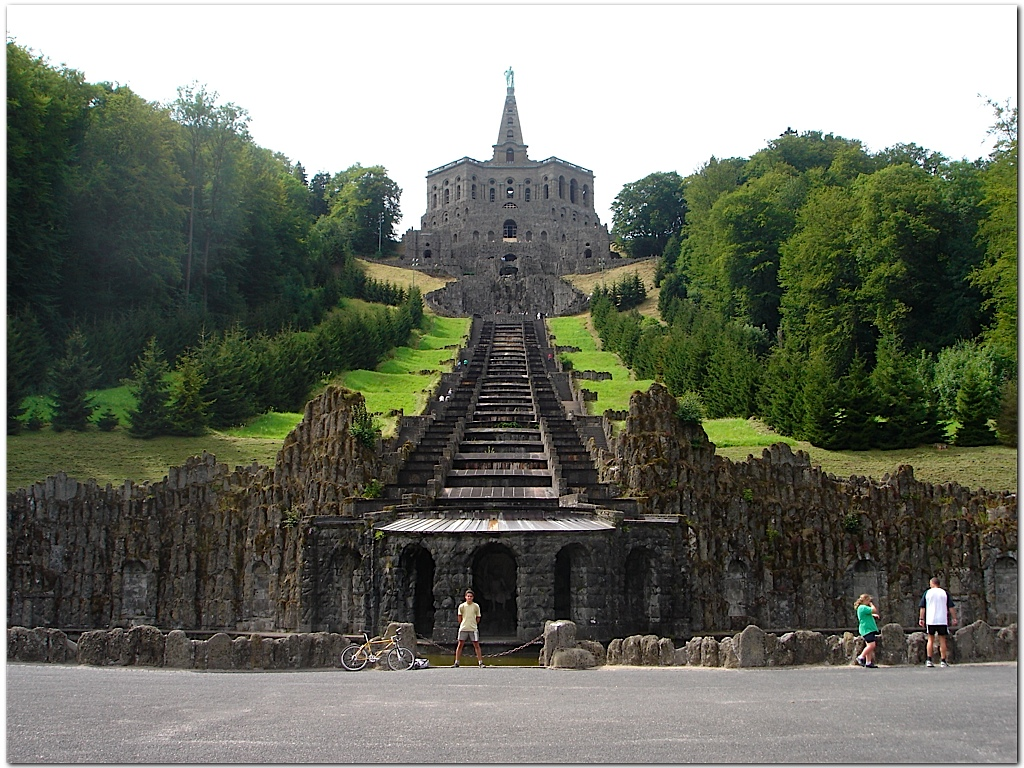
\includegraphics[width=300px]{images/DSC01248.jpg}\\ \textsc{Al
final de la colina, las escaleras al H'ercules.} \end{center}

Cuando llegu'e a la ruta entend'i porqu'e es mejor llevar bien infladas las
ruedas. \textexclamdown Iba muy r'apido, y las curvas se cerraban antes de que
las pudiera doblar! Las intentaba cerrar pero la bici se abr'ia solita, ten'ia
que frenar para poder entrar. Como en algunas curvas con bici cargada, es muy
raro sentir eso porque uno en bici siente que puede doblar lo que aparezca.
'Estas est'an con no mucha presi'on, y no las cambi'e para devolver la bici como
la encontr'e. Yo cre'ia que si segu'ia otra l'inea que la deseada me ca'ia
inevitablemente (el sonido de las cubiertas no da mucha seguridad), pero
descubr'i que no. La transpiraci'on envuelta en viento fresco no se sinti'o de
lo mejor, en todo el viaje esto, porque a la vuelta tuve viento de frente.

Volv'i en vez de por bici sendas (donde hay peatones) por la avenida, donde iba
a la misma velocidad que los autos, en sem'aforos m'as r'apido para no demorar y
divertirme. Fue incre'ible ver en instantes tan lejos al H'ercules, siendo que
para llegar lo estuve viendo a lo lejos durante casi una hora. En la ida hab'ia
medido la fuerza para poder volver a G\"ottingen sin morir en el intento (uno se
da cuenta cuando se est'a cansando o cuando va bien por esa cosquilla en los
m'usculos, que debe tener un nombre) pero la adrenalina de la bajada mezclada
con la emoci'on de haber llegado hac'ian que no la sintiera Us'e mucha fuerza
que se sinti'o bien, pero luego me dar'ia cuenta de que el tema no era llegar,
sino volver. Es obvio, ya lo sab'ia, pero en estos momentos no lo pensaba.

En libros sobre monta\~nismo encontr'e interesantes sensaciones respecto de la
llegada a una cumbre. Sebasti'an Letemend'ia, en ``Cita en la Cumbre'', relata
que all'i arriba no hay un gran alivio ni una fiesta, sino piedras, y el inicio
del descenso. Julio Godoy, en ``An'ecdotas de monta\~nas'', cuenta que al llegar
a la cumbre del Aconcagua sinti'o humildad. La meta es el viaje; la cumbre, una
bella consecuencia.

Hab'ia llegado a las 12 a almorzar, y a la 1:30 al H'ercules; tendr'ia que salir
a las 4 de vuelta a G\"ottingen si usaba poco m'as que las 3:30hs de la ida,
para llegar alrededor de las 8 a la cena. Quise tomar otro camino para conocer
otros pueblos, pero los cruces no eran f'aciles, y para no perderme volv'i de
nuevo por Hann M\"unden.

Com'i unas frutas, y par'e luego en una estaci'on para pedir agua y tomar un
helado ``Cornetto''. Los guachos dejan todo el chocolate en el 'ultimo bocado,
\textexclamdown se convierte r'apidamente en vicio! Sal'i a G\"ottingen despu'es
de enfriarme. La primer subida (\emph{larga}) y el viento se empezaron a hacer
notar. En el camino me detuve de nuevo para ver los aviones. \textexclamdown Los
quer'ia ver mientras pedaleaba y casi caigo al r'io! Despu'es de mucho pedalear
(\textexclamdown c'omo se siente ahora! Fueron 20~km) llegu'e a
``\emph{M\"unden}''. Com'i otro gran helado, y le agregu'e un chocolate
caliente, tentado por un vecino de mesa. Estuve un rato sentado, pase'e poco por
la misma zona que la 'ultima vez con Gustavo y segu'i viaje.

Restaban 30~km, ahora sufridos. Sin saber si llegaba, muerto del cansancio,
sucio, con transpiraci'on fr'ia por el viento en contra, cambiando siempre
velocidades cortas y livianas, dos caminatas\ldots\ Nunca llegaba la bajada,
todas eran subidas. Lleg'o a importarme todo un r'abano, y si llegaba a las 10pm
me daba igual.

Ped'i agua de nuevo a 15~km, y poco despu'es, luego de unas interesantes curvas
por un bosque, por fin la bajada. \textexclamdown Estaba tan contento!
\textexclamdown Ya se ve'ia G\"ottingen! Si el desaf'io era volver,
\textexclamdown casi lo ten'ia! Los kil'ometros se empezaron a pasar solos, no
pedale'e mas. Ni siquiera me manten'ia sentado, porque muy buena bici esta, pero
el asiento es incomod'isimo. As'i que parado, inm'ovil hice 5~km yo creo,
invalorables ahora. Nunca hice tantos~km juntos en un mismo d'ia, s'olo en la
gran bajada chilena, que era casi f'acil.

Llegu'e a zona urbana y hasta que encontr'e la casa de Gustavo, otra eternidad.
\textexclamdown Qu'e profundo cansancio! Se me cerraban los ojos, me dol'ia
hasta el cuello por la posici'on de la bici. Lo bajaba para estirarlo pero era
peligroso para seguir la l'inea. En un momento mis piernas no estaban c'omodas
ni movi'endose, ni quietas; malestar general.

Al llegar, la euforia. \textexclamdown Pude! Quise elongar y se me imposibilit'o
porque me acalambraba de s'olo intentarlo. Me felicitaron, Gustavo me ret'o
suave por no llamar (\textexclamdown Ina debe haber sido primera, porque fue
quien no quiso que vaya!), y me ofrecieron un ba\~no de inmersi'on arriba. Es
una tina de las largas, en que uno entra entero, con agua hirviendo. Hirviendo
literalmente, porque en cuanto met'i el primer pie (sucio y congelado por el
viento fr'io) me sali'o humo por las orejas. La enfri'e un poco, y al meterme
sent'i una inyecci'on de relajaci'on. \textexclamdown Por fin pod'ia dejar
no-tensas las piernas! Y sumergidos en agua caliente, despu'es del fr'io y la
suciedad. Un placer enorme. Decidido: mi casa tendr'a una tina de ba\~no larga
como yo (como 2,20m).

Me llamaron para cenar. S'olo sopa hab'ia, \textexclamdown y parec'ia tan poca!
Pero ya hab'ian comido estos tempraneros (con raz'on la inquietud de si llego o
no llego) as'i que para m'i solo, ahora, era mucha. Com'i un mont'on\ldots\
com'i mucha gelatina despu'es. Al llegar, com'i bastante pan. Y en vez de tomar
agua tom'e un jugo hecho por Ina m'as dulce que la granadina. \textexclamdown A
reponer energ'ias y nutrientes! S'olo en viajes largos me sobrepasaba tanto. Que
no se me hayan vuelto a acalambrar las piernas, y que hoy no me duelan, ser'a
(creo) por ese relajante ba\~no. Hizo un cambio instant'aneo en c'omo las
sent'ia. Me acost'e a las diez, y a las 10:01 me dorm'i. Si lo escrib'ia ayer lo
escrib'ia m'as sentido todav'ia yo creo. \textexclamdown O m'as exagerado,
siendo sincero!\\

Otros comentarios que quiero recordar, m'as all'a de este viaje:

Ina prepara el jugo. Es de un fruto m'as 'acido que la granada, que se saca de
arbustos. Rojo y del tama\~no de granos de granada. Se comen s'i o s'i con
az'ucar, y el jugo es tan dulce como la ya mencionada granadina. \textexclamdown
Rico y poderoso!

En las bici sendas, por la ciudad, parece no haber bocacalles. Los autos miran
si est'a por pasar alg'un ciclista, y frena en caso afirmativo. Uno toma la bici
en la casa, y no da vuelta la cabeza ni frena hasta llegar a donde quiera. Me
acuerdo de ir con Ina en su auto por una avenida, y fren'o bruscamente antes de
una rotonda, sin que haya peatones. Por la vereda nos acompa\~naba una bici, que
al final cruz'o sin mirar porque as'i es como est'a supuesto.

Se ven menos fumadores que en Espa\~na (casi ninguno), y muy pocos celulares.
Para ser sinceros s'olo vi 4 ``celus'', de gente rondando los 20 a\~nos.
\textexclamdown Casi nada! Yo cre'i que ser'ia al rev'es con los celus, como
est'a explotando all'a. A diferencia de Espa\~na tambi'en, se ven algunas
camionetas.

Los colectivos, al abrir las puertas, bajan las suspensiones de la derecha para
acercar a la persona al suelo. Al cerrarlas, vuelve a subir. La idea es simple
con suspensiones neum'aticas, pero verlo es de ciencia ficci'on.

Al entrar en los bosques se percibe notoriamente el cambio de temperatura. Se
siente el aire un poquito m'as fr'io.

Creo que no olvido nada interesante. Hoy seguir'e descansando, y ma\~nana
recorrer'e alguna cosa nueva. Ya estoy mirando con cari\~no el mapa, mirando
otros pueblos cercanos a G\"ottingen. \textexclamdown Hasta se ve Bettenrode,
que son dos establos para equitaci'on!

\subsection*{Domingo, 7 de Agosto}

Hoy me levant'e temprano, desayun'e mucho como siempre, y sal'i en bici para el
Noroeste, pues siempre para el Sudeste u Oeste sal'ia G\"ottingeano. Como
notar'an ahora llevo mapa, de esos para bici que no importa si se mojan. No me
ayuda mucho a seguir los pueblos que quiero porque en general me pierdo en
cruces, pero est'a bueno para saber si estoy muy lejos o no, y calcular el
tiempo de vuelta. Perderse significa llegar a un cercano pueblo de diferente
nombre, con quince caminos que lo unen a otros. No es la gran cosa ``perderse''.
Hoy sal'i a las 9:30 y a las 13:30 ten'ia que estar de vuelta para el asadazo de
Gustavo. \textexclamdown No se extra\~na eso!

Se ve'ia siempre lejana pero amenazadora una gran nube negra, y estaba todo muy
oscuro. Tuve varias lluvias pasajeras intercal'andose con el sol.
\textexclamdown Parec'ia el pato Donald con la nube de lluvia solamente sobre mi
cabeza! Pero no me moj'e mucho, y saqu'e fotos no tan interesantes por el
paisaje, sino por c'omo se ve el cielo con tanto cambio de clima. Para este lado
los pueblos son muy pintorescos. Antiqu'isimos, bien conservados, siempre el
mismo lindo estilo, siempre la gran capilla en el centro de las casitas, que
desde lejos destaca el campanario. Bonito.

Quer'ia llegar al lago Seeburg See, en Eichsfeld. A la izquierda de mi camino me
sorprendi'o lo oscuro de un gran bosque: era incre'ible ver un sol radiante en
la entrada, y no poder ver m'as de tres filas de 'arboles adentro por la total
oscuridad. Por sobre la senda entraba la poca luz de ese d'ia.

Est'a bueno entrar en bosques porque uno no piensa cu'anto tiempo o distancia
avanz'o, uno se limita a avanzar mirando a los costados, adelante, y un poquito
hacia atr'as. Es como un teletransporte entre entrada y salida: uno no piensa
cu'anto tiempo pas'o/pasar'a hasta llegar a donde quiere. En cambio en las
colinas uno ve cambiar el paisaje y acercarse otros pueblos, y piensa cuantos
kil'ometros habr'a recorrido. \textexclamdown Todo tiene su belleza! Agrego que
al acercarse a los bosques en bici uno puede escuchar la lluvia, aunque no
llueva. Las gotas que quedaron en ramas y hojas siguen cayendo luego con el
viento, el sonido contin'ua. Qu'e paz, la Naturaleza.

Despu'es de subir bastante por el bosque --sin darme cuenta por supuesto--
llegu'e a una recta en bajada. Entre la falta de sol para secar el camino y las
nubes de lluvia pasajeras, estaba tan mojado que no ve'ia nada mientras bajaba.
Adem'as el viento de la velocidad me hac'ia llorar. S'olo miraba bien cerquita
de la rueda, para saltar algunas canaletas que cruzaban. De repente se empez'o a
ver luz al final del camino, ser'ia el final del t'unel de vegetaci'on, pero
cuando vi con m'as atenci'on encontr'e adem'as una valla que evita el pase de
autos. \textexclamdown Y no pod'ia frenar! Iba muy r'apido, la rueda de atr'as
entre patinando y levantada, y la de adelante no ``a tope'' con la presi'on.
\textexclamdown Malabares hice para no chocar!

Cuando la sorte'e despu'es de frenar al m'as puro estilo ``McGyver'', me
encontr'e, todav'ia, arriba de una sierra; desde donde se ve'ia Eichsfeld. De
fondo se ve'ia el torment'on; era el fin del mundo, de eso estoy seguro. Por
suerte el camino volv'ia en sentido contrario al de la tormenta.

Recorr'i las calles, siempre los mismos comentarios sobre caminos,
irregularidades por no urbanizar planificadamente, y edificaciones. Siempre lo
mismo pero siempre sorprende. Conoc'i el lago, que nada tiene que envidiarle al
de G\"ottingen, y tiene el turismo m'as aglomerado en un punto. Y emprend'i la
vuelta.

Me iba a alejar un poco, pero prefer'i llegar temprano para ba\~narme antes de
almorzar. No pas'e por muchos pueblos en esta vuelta, pocos y poco interesantes;
pero me met'i en un bosque de esos que teletransportan. Ni siquiera sab'ia si
estaba en el camino correcto y la verdad es que no me importaba. Cuando sal'i,
esas nubes pasajeras ya no estaban, y la gran tormenta estaba cerca. Como ten'ia
viento en contra supuse que se alejar'ia, pero a los pocos kil'ometros empec'e a
verla cada vez m'as cerca. \textexclamdown Pero cerca en serio! No m'as de diez
cuadras. Se ve'ia el agua caer as'i, en forma de nube: una pared negra a menos
de mil metros m'ios que avanzaba. Por una senda perpendicular se ve'ia tragar a
dos peatones y su perro. Y es que no era agua, porque en unos minutos un granizo
\emph{muy} finito me empez'o a picar todo el cuerpo. Par'e al lado de un pino
para resguardarme y al poco tiempo me empec'e a mojar igual. Mir'e mi buzo y
estaba lleno de esos granitos de granizo, toqu'e mi cabeza y lo mismo. Me los
quise sacar, y entre los derretidos y la lluvia\ldots\ \textexclamdown me
\emph{congel'e}! \textquestiondown Vieron lo que se siente al congelarse el
cerebro con helado, despu'es de la cena? (S'olo angurrientos.) Eso mismo. Era
divertido, aunque no se sent'ia nada bien.

Como me mojaba igual pens'e en seguir, pero el granizo picaba tanto que par'e
bajo un techo. Llov'ia torrencialmente, estaba oscuro el mediod'ia. Cuando dej'o
de caer piedras a los pocos minutos, segu'i andando en bici. Por suerte todo de
bajada segu'ia el camino, hab'ia elegido el que sube por los bosques y ahora
llegaba la recompensa. Iba rapid'ismo por una ruta en buen estado con buen lugar
para bicis y el agua saltaba a la cara casi picando, mientras el viento
congelaba toda la piel que encontrara. Pensaba en el ba\~no al llegar y me
relam'ia. La ruta tan linda se transform'o en una ``normal'', menos ancha y
llena de piedritas por mi l'inea externa, patinaba de lo lindo y no se ve'ian
los pozos que me daban un eventual baile. Senda para bicis no hab'ia por ah'i.
Si no me ca'i, no fue por otra causa que la suerte.

Es impresionante c'omo el fr'io hace perder sensibilidad y fuerza. Ten'ia las
manos duras del fr'io, y se me complicaba hacer los cambios. \textexclamdown Al
llegar no pod'ia abrir con una sola mano (desde la llave) una puerta! Al menos,
despu'es de andar tanto bajo la lluvia, la bici se limpi'o del barro que ten'ia.
Las cubiertas parecen salidas de f'abrica. No voy a tener palabras para
agradecerle a quien me la prest'o. \textexclamdown Espero no oxidarla!

Al llegar me di un ba\~no hirviendo, los pies y manos ard'ian. Cuando las manos
dejaron de arder, \textexclamdown sent'ian el agua fr'ia! La tocaba con el
cuerpo y estaba caliente, pon'ia las manos y se volv'ia a sentir fr'ia. Estos
d'ias fueron fr'ios en esta zona, el viento sobre mojado lo multiplic'o. Pobre
cuerpo, c'omo lo pongo a prueba. Y funciona bien: despu'es de unos minutos de
sauna me normalic'e, y almorzamos el asado de la vida.

A seguir leyendo pasivamente hoy, que las lluvias se intercalan con el sol.

\subsection*{Lunes, 8 de Agosto}

Hoy no me mov'i mucho de casa. Igual escribo varias cositas para no olvidar.

A la ma\~nana a las oficinas, despu'es del grande desayuno. Cada vez me gusta
m'as, \textexclamdown hasta me dan ganas de desayunar a la tarde! Un pan con
semillas, gris pero rico, con manteca y mermeladas caseras. Y un ``buen t'e
argentino'' (\textexclamdown se lo traje y lo acabo antes de irme, sin dudas!)
con leche.

Al mediod'ia, y en un intento de regalarle la Gran Selva Amaz'onica a la Virgen,
llevar'ia a Pablo (Felipe anda medio enfermo) a la \emph{Kinderstadt}: un lugar
para que quemen toda la energ'ia que acumulan durante los minutos del desayuno.
\textexclamdown Qu'e intolerante me veo al escribir sobre ellos! No se preocupen
que no los trato tan as'i. Pero es verdad: la ciudad de los chicos tiene juegos
t'ipicos como saltos en trampolines, y no se qu'e m'as porque por suerte no
conoc'i. Es que mientras almorz'abamos lo invit'o un amigo a la casa, y
prefiri'o jugar con 'el. Pero la verdad, divino Pablo, cuando salgo me dice,
sosteni'endome las manos: ``Esto no puede ser, \textexclamdown ven'is a Alemania
y no te vemos nunca!'' Tierno le queda muy corto.

As'i es que despu'es del almuerzo fuimos con Ina a comprar mapas alemanes para
este otro nene, el que escribe. Se me cae la baba, \textexclamdown son
\emph{inmensos}! Son del ``{\small ACA}'' alem'an ({\small \emph{ADAC}}), varios
gratis, y los grandotes pagos.

De ah'i a una jugueter'ia para que Pablo compre un regalo a un amigo que cumple
a\~nos. Cuando Ina, para irse por fin, encontr'o a Pablo\ldots\ \textexclamdown
no me encontraba a mi! Y menos mal que Felipe dorm'ia en el auto. Yo estaba
hipnotizado por la cantidad de ``Playmobil'' que hab'ia. Despu'es de a\~nos me
agarr'o la nostalgia y compr'e dos hombrecitos vestidos de caballeros para que
adornen mi escritorio a la vuelta. De paso me recuerda a los castillos conocidos
y por conocer. \textexclamdown Est'an buen'isimos! Son dos mu\~nequitos simples
pero muy valiosos: juguetes de ni\~no, y caballeros europeos.

De ah'i a pasear haciendo otros mandados y a casa, donde arm'e los mu\~nequitos,
termin'e de mirar el cat'alogo 2005 Playmobil, e intent'e armar un castillo
``play'' con los chicos, de estilo alem'an.

Despu'es me qued'e cuidando a los chicos, y se portaron muy bien. No saben qu'e
nervioso me pon'ia porque tienen cajas y cajas de juguetes, pero quer'ian jugar
con mis dos humildes mu\~nequitos. \textexclamdown Y esto despu'es de hacerles
entender que no era un regalo para ellos, mientras los armaba! Se me perd'ia una
espada de pl'astico y mor'ia, as'i que los guard'e en mi bolsillo y me pincharon
todo el d'ia. \textexclamdown El pago por mi egoismo! Cuando logr'e dejarlos con
\emph{sus} juguetes, me puse a mirar los mapas en la mesa, despu'es de cenar
comida ``t'ipica de la selva negra''. Nada del otro mundo, s'olo forma
diferente.

T'e de por medio, abr'ia la inmensidad de los papeles junto con los mails de mis
t'ios y me deleitaba\ldots\ \textexclamdown Qu'e lindo es abrir mapas!
\textexclamdown Mientras m'as grandes, mejor! Cuando vaya a El Calafate me voy a
comprar uno de toda Am'erica. Y una mesa de 5m de largo para caminar alrededor.
Organic'e a grandes rasgos un viaje por la Selva Negra, sudoeste alem'an, pero
entre cada pueblo hay \emph{tantos} otros peque\~nitos que no s'e por qu'e
camino unirlos. Mando detalle a los organizadores de confianza. Otros me dir'an
que me quede en la \emph{Oktoberfest} de Munich. Es medio loco pero seguramente
interesante. Dicen que lo ``malo'' es para las mujeres no para los hombres.
\textexclamdown Por ah'i viaje en bici! El tema es cu'al. Ver la escala de los
mapas es alentador, \textexclamdown las distancias son tan cortas entre pueblo y
pueblo! Aunque me informan de lo monta\~noso del relieve. Otra cosa: me
imaginaba que entre Alemania e Italia se interpon'ia \emph{toda} Europa,
\textexclamdown pero est'an ah'i nom'as! Tengo pa'ises al rededor para tirar
para arriba. Voy a volver hablando checo me parece.

Ayer Domingo, con el fr'io total, encendimos el hogar, que est'a en el centro
del living. \textexclamdown Un poco para usar los 3m$^3$ de le\~nas que compr'o
el due\~no de casa, otro poco por fr'io! No saben lo que fue ordenarlas, ya
tengo cayos de gaucho. En mi casa voy a tener, exactamente, esa ubicaci'on
central del hogar. Aunque no se vea la cara de quien se sienta en frente ni el
televisor. Uno apoya los pies sobre el hogar y dan ganas de mover la cola como a
un perro. Y ac'a andamos descalzos, una gloria. Ya jete'e pantuflas a los padres
postizos porque se me engangrenan los pies.

Empec'e a rasgu\~nar palabras en alem'an, como para hacerme entender, aunque sea
a lo indio. Nada de nivel, pero ese peque\~no ara\~nazo seguro me va a salvar en
varias situaciones. Gustavo me indicaba que el alem'an es un idioma muy rico y
espec'ifico, que hace complicado el aprendizaje pero placentero su uso. Me
llamaba m'as la atenci'on para aprenderlo, pero no las ganas de estudiarlo.

\textexclamdown Termin'e ``El Alquimista''! Me gust'o much'isimo, tienen raz'on
quienes comparan el estilo con El Principito: simple ``para ni\~nos'', con un
gran contenido de fondo. Lindos libros, realmente para todo el mundo.

Mis mu\~nequitos me est'an mirando, siempre sonriendo porque no existe playmobil
sin sonrisa. \textexclamdown A pesar de amenazarme con sus armas y armaduras
parecen amigables! Y a pesar de tener escudos y colores diferentes. Este nene
con chiche nuevo se va a dormir.

\subsection*{Mi'ercoles, 10 de Agosto}

Por d'ias lluviosos no tan cambiantes como siempre, estuve bastante adentro.

Termin'e de leer ``Stalingrad'', libro crudo como pocos. En realidad s'olo narra
esas batallas durante la m'axima expansi'on del imperio Nazi y sus
consecuencias, pero como bien dice una cr'itica ``es s'olo lectura de noche para
quien no sue\~na''. Es el odio entre personas hecho cosa, tangible.
\textexclamdown Querer el mal! Masoquismo. Bruto. El que lideraba todo el
ej'ercito 6$^{\circ}$ (alem'an) en la Uni'on Sovi'etica, general Paulus, fue
tra'ido en el a\~no 1.955 a Alemania, muy avejentado despu'es de tanto estr'es.
Lo enterraron junto a la mujer en \emph{Baden-Baden}. \textexclamdown Qu'e
casualidad! Me dir'an: ``es que est'as en Alemania'', pero en breve, si todo
sigue como viene, visitar'e \emph{Baden-Baden}.

Empec'e un libro de Gabriel Garc'ia M'arquez que me encant'o: ``12 cuentos
peregrinos''. Es un buen estilo de escritura. Por si encuentran en internet, 4
hojas ocupa ``El avi'on de la bella durmiente'' y es muy entretenido y gracioso.
Y ma\~nana salgo para la librer'ia en ingl'es as'i clavo alg'un otro, tengo
varios t'itulos en mente, ver'e por cual me decido.

Hoy, la familia menos Gustav, fuimos a pileta techada. Los 20~km en auto fueron
por caminos ya conocidos. La pile con sales ten'ia m'as sal que el mar, me
sumerg'i y al abrir los ojos arriba me ardieron por 40mins. \textexclamdown Pero
por fin no se hund'ian las piernas al hacer la plancha! Quise llegar a tocar el
piso de la pile de nataci'on, 3,40m, mientras Ina me indicaba. A los 2 metros me
molestaban los o'idos y ten'ia que subir. Ver la superficie desde abajo mientras
se sube es como estar volando, uno va a donde quiere en las tres dimensiones. En
una pile era divertido, no imagino en mar abierto. Estaba un poco nervioso y por
eso (y por resfr'io, seg'un ella) no me sal'ia un ejercicio para compensar las
presiones en los o'idos. No creo que un buzo resfriado no se sumerja, aunque
ella dijo que s'i. \textquestiondown C'omo se sentir'an los ``escasos'' 20
metros, por ser buzo ``amateur''? No veo la hora de empezar los entrenamientos.

Ma\~nana por fin salimos en bici en la madrugada con Gustavo. Para hacerlo, en
vez de ``despertarnos mutuamente'' (que se trataba de esperar al otro mutuamente
para dormir ``otros cinco minutos''), esta vez tomo las riendas y lo levanto yo.
Me llega a decir que no, y lo tiro por la ventana con frazadas y todo. Al
empezar ser'a un embole pero despu'es, seguro, va a ser divino. Si no llueve. Si
lloviera tambi'en ser'ia divino pero ya es otra excusa m'as para no hacerlo.
Para correr no importa la lluvia, pero en la bici uno se congela.
\textexclamdown No prueben en casa que ya experiment'e!

Hoy me volv'i a quejar del pelo largo e impusieron mano dura: Ina tom'o las
tijeras y me lo achur'o. Debe haber sido placentero para ella. Para m'i
tambi'en. Est'a bastante prolijo (\textexclamdown ahora se peina para atr'as!).

Gustavo me tiene cansado con su indecisi'on para cambiar el auto. En vez de
comprarse un ``barato'' (y alem'an) Passat, busca en Nissan, Renault, Peugeot
(buena idea con el 407). Pero como ac'a el Passat es auto de polic'ia y taxi
(``joya-nunca-taxi'' no se aplica ni en Mercedes Benz en Alemania) no se ve como
\emph{la m'aquina} que es. Los Audi A4 Avant a veces son bomberos, a veces
ambulancias. No la vi pero s'i en foto: una Porsche Cayenne ``trabaja'' para los
bomberos de una ciudad. \textexclamdown No se conformaban con un todo terreno
``com'un''! Es que en Alemania creo que no se producen.

\subsection*{Jueves, 11 de Agosto}

A la ma\~nana, a las oficinas. A charlar un rato en ingl'es, se siente bien. Una
colega no odia pero tampoco gusta de Alemania. Cuando me habl'o (\textexclamdown
juro que ni mencion'e el tema!) de autos nombraba italianos. Dios le da pan a
quien no tiene dientes. En su no-amor por la patria, no puede creer que vaya a
recorrer por semanas la Selva Negra. \textexclamdown No sabe que yo tampoco lo
puedo creer!

A la tarde fui en bici al centro. Iba por una calle cuando un polic'ia de civil
me hizo se\~nas de que aminorara. \textexclamdown Hasta las bicis son
controladas en este gran pa'is! Gustavo me indic'o que si me pillan por la
vereda debo pagar multa. Ayer est'abamos mal estacionados y un
Passat, para colmo, se mand'o en contramano. Cre'imos que estaba re-perdido,
pero era otro polic'ia de civil, controlando. Sac'o la medallita que lo
acreditaba, y nos urg'ia a movernos o a pagar una multa.

Recorr'i librer'ias que no me atrajeron, y fuimos a un pueblo que cre'ia
lejos pero cercano al fin. Viajamos Gustavo, hijos y yo en el {\small BMW}.
Ellos se quedaron a hacer un tr'amite, y yo sal'i a caminar. Unas turbinas
e'olicas me indicaron que ya hab'ia recorrido por ah'i, volviendo a
G\"ottingen desde \emph{Seeburg See}. Sin embargo segu'i caminando y confirm'e
que en Alemania no hay que viajar en bici sino a pie. En la bici observaba las
turbinas, a pie \emph{todo} lo dem'as. Conoc'i un molino de viento ``a la
antig"ua'', de esos holandeses, y dos molinos hidr'aulicos. Muy antig"uos e
interesantes. C'omo se las ingeniaban antes con esos materiales es admirable.

Al atardecer ten'ia pensado salir a correr por los bosques, pero entre tantas
vueltas para volver (entre otras a ver un Honda Accord, otro no-alem'an que me
gusta bastante) me olvid'e y com'i todo al llegar. El fr'io me indic'o el camino
a la ducha cuando Gustavo me interrumpi'o: ``\textquestiondown salimos o no?''
Mi piel de gallina le habr'a contestado. \textexclamdown Y la cara tambi'en!

Luego de leer un mont'on de buenas noticias argentinas, le dije a un amigo:
``disfrut'a por m'i'', y me contest'o: ``disfrut'a vos por todos nosotros,
\textexclamdown huev'on!''. \textexclamdown Qu'e alegr'ia! \emph{Todas} buenas
noticias.

\subsection*{Viernes, 12 de Agosto}

La vieja hoy se emocion'o al tel'efono por escuchar mi ``hola'', me demostr'o lo
poco que llamo\ldots\ \textexclamdown Menos mal que existe internet al menos!

Ayer a la ma\~nana, como me promet'i, sal'i a correr al bosque. Me acompa\~n'o
Pablo en su bici, cre'i que tendr'ia que seguirlo como el burro a la zanahoria
pero fue al rev'es, as'i que a la vuelta no anduve todo lo que quer'ia, y
trabaj'e un poco (\textexclamdown alg'un d'ia!) arriba de la cintura.
\textexclamdown Todav'ia me duelen los m'usculos por la falta de costumbre!

A la tarde fui a la joyer'ia para almorzar con Gustavo y una amiga que
me presentaba, Lissy, quien quer'ia almorzar en no-se-qu'e lugar. Yo me hab'ia
olvidado, y ya hab'ia almorzado en casa, y bastante luego de la ma\~nana
deportiva. Cuando llegamos era un lugar medio vegetariano aunque no del todo, de
alimentos livianos y saludables. Para tomar: jugo de naranja exprimido. ``A Dios
gracias'', se le escap'o en voz alta a mi pancita satisfecha; empezamos el
almuerzo riendo. Divina la chica, muy simp'atica. Ser'a quien me ense\~ne
alem'an. Ella me va a ayudar porque me tiene como chico pa' la escuela.

Hablando de aprendizaje, Ina me regal'o hoy unos cursos que creo van a servir
mucho. Ahora se juntar un verbo con una persona. En ingl'es uno dice
I-you-we-they (alguno) + verbo. Pero ac'a para cada persona hay conjugaci'on
distinta, como en castellano. \textexclamdown Qu'e bueno si llego a mantener
un di'alogo de cinco l'ineas con alguien! Seguro si lo quiero.\\

Esta ma\~nana Gustavo se puso firme consigo mismo y me levant'o a las 6:30 am.
Como estaba el piso mojado y un poco fr'io le suger'i que dejemos las bicis y
salgamos a correr. Ir'iamos al lago. Cuando lo vi cinco minutos despu'es estaba
disfrazado de astronauta, no pude evitar sacarle una foto y se re'ia en vez de
putearme. Corr'i \emph{muy} bien, se nota que el clima fresco ayuda porque
hac'ia tiempo no corr'ia as'i. O ser'a porque en el lago no existen las
pendientes que pueblan los bosques. Una madrugada corriendo en el lago, si bien
hac'ia fr'io (y con sue\~no) fue de lo mejor. Al lado del camino 5 cisnes se
acicalaban retorciendo el cuello por todo su cuerpo. Me desvi'e unos metros para
correr un poco por entre bosques, donde de nuevo se escuchaba lluvia almacenada,
sobre piso blando lleno de hojas y ramas ca'idas.

Dorm'i una tremenda siesta (hoy no me duermo m'as) y comimos un asado de lujo.
Gustavo hace el pollo tan rico (pero con su sabor particular) como ``Las
Brasas''. Siempre se acuerda de aquella esquina, y tiene un im'an en la
heladera. Le dije que pidiera por tel'efono, pero ya intent'o seg'un dice.

Dej'e un libro de historias cortas en ingl'es que me embolaba, porque me atrap'o
instant'aneamente ``Fahrenheit 451'', de Ray Bradbury. Dice Gustavo que es un
cl'asico y as'i parece, pero no lo conoc'ia. Las palabras ``451$^{\circ}$F es la
temperatura a la que los libros arden'' abren la obra. Cada hoja es incre'ible,
imperdible. Reci'en lo empiezo. \textexclamdown Y con mi insomnio por siesta hoy
lo termino!

Ando con problemas para conseguir bici para mi viaje. Dice Ina que la
'ultima es comprar una, usarla y revenderla: ser'ia m'as barato que alquilar. Y
bueno, si lo tengo que hacer lo hago porque s'e que no va a tener precio ese
viaje. Y la bici no tiene por qu'e valer \geneuronarrow{1000}. \textexclamdown
Si con \geneuronarrow{980} me alcanza!

\subsection*{S'abado, 13 de Agosto}

El s'uper-despertador controlado por radio frecuencia me levant'o tipo 7:30 con
un piripip'i suave, que despu'es se transforma en el enfermizo y conocido sonido
de todo despertador. Quienes trabajan lo conocer'an, \textexclamdown yo lo
conozco porque me contaron! Desayun'e no mucho porque iba a la pileta, esta vez
a nadar y no a divertirme un rato.

Como no s'e otro estilo, nad'e como madre: rana. Lissy le llama estilo
``house-wife'', el mismo machismo de voz femenina. A las 8:30 la encontr'e en un
d'ia lluvioso. Fuimos a piles techadas excepto una, todas climatizadas. La de
afuera largaba humo bajo una fina y fr'ia lluvia. Y el precio muy barato. Ya
adopt'e la relaci'on euro (menos mal que lo tengo a Gustavo porque sino hoy me
compraba una bici, despu'es cuento). La guacha me dec'ia que mejor a'un es
cuando nieva para nadar afuera.

Abren las piles tipo nueve, y llegamos nueve menos cuarto. Entre el
``\emph{check-in}'' y preparaciones se hicieron las 8:55, y nos tuvieron
exactamente 5 minutos junto a otras \emph{house-wife} para que se hicieran las
9:00 (cero-cero), y poder hacer uso de las instalaciones. ``T'ipicamente
alem'an'', dec'ia Lissy entre dientes. Yo disfrutaba de la perfecci'on, hecha
obsesi'on. La tarjeta duraba hasta las 10:00 (cero-cero).

Como esperaba, a los diez minutos estaba bastante cansado. Se usa mucho la
espalda. Diez minutos m'as, y salimos. Pens'e en no volver: no es un deporte que
me encante, pero ella propuso como objetivo llegar a los 40 minutos
``\emph{non-stop}'', como pod'ia hacer antes. Mi orgullo va unido a los
desaf'ios con plasticola, as'i que ir'e durante la semana con Ina (Lissy trabaja
mucho), para llegar a hacerlo. \textexclamdown Qu'e divina! No se hace un
problema: hoy la invit'e y contest'o un decidido ``\textexclamdown claro!''\\

Dorm'i una peque\~nita siesta y me levantaron los chillidos de los chicos. Y con
el atontamiento del sue\~no no era precisamente un 'angel al bajar. Despu'es de
comer unos panes con manteca fuimos a un restaurante chino. D'ia lluvioso, el
'ultimo detalle.\\

Este fue el punto de inflexi'on: el restaurante chino, interesante y adem'as
hermoso. El almuerzo, riquis'isimo; los chicos, angelitos totales durante el
almuerzo. Cuando terminaron jugaron con unos mu\~necos nuevos. Charla divertida
con Gustavo medio copetineado decor'o la sobremesa, en la que tomamos t'e de
jazm'in, que est'a bueno. \textexclamdown Me cont'o que cambiaron el nombre de
calle ``guardavieja'' de Buenos Aires, por ``cuidado, mam'a''! Y tom'e una
cerveza Warsteiner que me gust'o.

A la salida recorrimos varios pueblos. Me mostraron una ruta para visitar en
bici que no conoc'ia, con varios poblados tan pero tan lindos, y caminos
\emph{tan} pintorescos, que no dudo voy a volver. Me contaban que los rusos en
su guerra no destrozaban las ciudades, peleaban m'as cuerpo a cuerpo. Los
ingleses y americanos bombardeaban y listo, cosa que hizo perder mucho encanto a
los pueblos occidentales.

Visitamos un castillo, y la frutilla del postre fue a la vuelta, en una parada
en lo que ser'ia algo as'i como una estancia alemana. Por tama\~no no se le
puede llamar as'i. Es un para'iso. Una familia poderosa alojaba a todos los
trabajadores (siglo {\small XVIII}) en un gran campo de ah'i. Es antigua, bella,
t'ipicamente alemana, y sostenida porque la gravedad es buena (techos como
paredes, inclinados). Paramos porque les hinch'e hasta el cansancio con que
quer'ia tomar un chocolate caliente en un lugar antiguo. No por el sabor
(dec'ian que era malo) pero por el lugar. Tomar un chocolate en esas casas
multiplica su calidad. Ten'ia un lago, decenas de gansos, varias construcciones
\emph{Fachwerkhaus}, un caf'e a la antigua, los ba\~nos cerca de los establos.
Moza y madre cajera que parec'ian caricaturas de alemanes t'ipicos. Por los
ba\~nos hab'ia una escalera bonita que sub'ia. Sub'i y llegu'e a un 'atico
vac'io tan antiguo que desentonaba con la escalera. Las telas de ara\~nas en los
escalones eran blancas y densas; ten'ian madre ara\~na y todo. Iluminada
l'ugubremente por peque\~nas claraboyas que tienen los techos a dos aguas, con
olor a tierra y humedad, llena de goteras que se escuchaban y sent'ian. Una
silla por ah'i y el piso de madera chirriando a cada paso. \textexclamdown De
novela! Har'e ese camino largo seguro, y lo repetir'e corto siempre que pueda,
como cuando voy a la olla. \textexclamdown Y si me alcanza el tiempo que se
esfuma!

Cuando volv'iamos pasamos por una bicicleter'ia. Par'o Gustavo para solucionar
mi 'unico problema para mi viaje en bici por el sur. La bici en cuesti'on era
casi igual a la segunda y mejor que tuve, robada al poco tiempo, a
\geneuronarrow{600}. Gustavo la quiere comprar en un instinto paternal al ver mi
emoci'on, justificado porque 'el la va a usar: ``ya me van a robar la que tengo
y quiero una todo terreno''. Llega a andar en una bici sin luz ni guardabarros y
se espasma; la va a revender seguro, pues es m'as barato que alquilar. Pero
quiere, porque le empec'e a explicar los palos que me pegu'e con esa bici por no
conocer por ser nueva (gracias a Dios en invierno, con campera, mochila y
guantes), c'omo me volv'ia de la escuela, c'omo frenaba en las esquinas bajando
cambios con la rueda trasera girando loca\ldots\ me puse euf'orico e
insoportablemente inquieto. La pobre Ina nos llam'o del auto porque se ahogaba
(trabas para ni\~nos, \textexclamdown viajo adelante!) y en el viaje le segu'i
contando de la bajada de los caracoles chilenos, y de las carreras por la
avenida con Eze los domingos en la tarde, con todo dominguero que exist'ia dando
vueltas a 15 y nosotros a 40. Y hablamos entonces de las casualidades que se
juntaron para que yo siga vivo despu'es de tantas locuras de joven inmortal
(siempre hablamos de casua-causalidades y de religi'on) y yo me pon'ia cada vez
m'as inquieto. Estaba tan molesto con estar quieto (euf'orico en realidad, de
nuevo) que mientras los limpiaparabrisas andaban decid'i salir a correr. Gustavo
me mostraba como ejemplo para Pablo: ``\textquestiondown Ven? Tute est'a
inquieto, se da cuenta, y sale a hacer deportes.'' Llegamos, tom'e agua y com'i
media pera jugosa, me cambi'e, \textexclamdown y a los bosques!\\

Trot'e como caballo por suave y por tiempo. No me quer'ia matar tanto (me
desgast'e como en Gij'on). Pero haber llegado a casa luego de casi dos horas, y
de la subidita del camino sin parar fue perfecto. Hice paradas para ver paisajes
al ver luz en la salida de los bosques, y serenidad en el trote. \textexclamdown
Y me quejaba de c'omo ``perd'i'' el estado!

A la media hora de salir por caminos desconocidos, y pensando que me alejaba,
volv'i al punto inicial de los bosques, a diez cuadras de bajada a casa. Pero la
``inquietez'' no se hab'ia ido, as'i que me met'i de nuevo por otros lugares.
Mientras iba por un camino angosto y muy patinoso escuch'e a varios metros un
movimiento r'apido entre la vegetaci'on, di vuelta la cabeza nervioso, y
encontr'e un ciervito salvaje, m'as asustado que yo. Naturaleza.

Esta vez me alej'e en serio, y sal'i, para mi sorpresa, por el otro lado de los
bosques. Pensar que Pablo al verme ir me dijo: ``no te vayas\ldots'', y yo le
respond'i: ``\textquestiondown Me acompa\~n'as al bosque?'' \textexclamdown
Menos mal que me mir'o con cara de traste, porque encima de esperarlo, perderme
con 'el hubiese sido terrible! Pregunt'e luego de pasar establos a un
colectivero el camino a G\"ottingen, y contest'o: ``l'inea 1''. Con no peque\~na
sonrisa le hice entender que quer'ia volver corriendo, y cuando dijo un
tranquilizador ``derecho'' me alej'e, suaveciito suavecito. Entr'e a G\"ottingen
por la otra punta, la avenida \emph{NicolaiStrasse}. Rodeada por palacetes
hermos'isimos, de tres o cuatro pisos, bien alemanes y tan viejos como
conservados. Tipo el Barrio Parque de Buenos Aires, pero con casas a'un m'as
viejas y grandes.

Por el centro de G\"ottingen era un atorrante, con todos elegantes saliendo a
pasear, y yo embarrado, sudando, con cara rojiza y pidiendo aire, medio en bolas
y mojado por la lluvia. Corr'ia sobre los charcos como un ni\~no para limpiar el
barro de las zapatillas. La remera de ``Orgal'' que us'e hasta de repasador en
Mendoza no ayudaba, y, si la quieren completa, sal'i con la 'unica malla que me
traje, color marr'on. Ma, \textexclamdown se te escap'o la tortuga ah'i con el
control del equipaje!

Todo esto fue bajo lluvias pasajeras, sea por los 'arboles del bosque que la
almacenan o por nubes. El agua saltaba bajo mis pies, si no patinaban, en cada
paso. Me embarr'e atr'as como si hubiese ido en bici. Vivir cerca de un bosque
no debe tener desperdicio. Los caminos nuevos nunca se deben acabar, as'i de
numerosos son los cruces.

Llegu'e m'as tranquilo que en el auto pero igualmente contento. M'as, porque me
siento mejor corriendo, y habiendo llegado a hacer algo que cre'ia no poder.
\textexclamdown El ``no puedo'' es odioso! El coraz'on ya no se dispara en las
subidas. La respiraci'on se mantiene. Elongu'e mejor tambi'en, moverme tanto
ayuda a la elasticidad. Y vine a escribir, para que no se me olvide nada.

Bueno, los dejo casi alegremente. Casi porque ma\~nana llega Axel, el due\~no de
``mi'' bici. Sab'ia que ma\~nana me desentend'ia de la bici pero hoy me acord'e,
despu'es de correr y de ba\~narme, que la tengo que dejar \emph{impecable} como
me la dio. Me sorprendi'o lluvia, barro, piedras del asfalto\ldots\ va a estar
dif'icil pero no puedo hacerlo de otro modo. As'i que ahora o ma\~nana en la
ma\~nana a limpiar. Y a averiguar otros precios de bici por G\"ottingen para
asegurar el buen precio de aquella de hoy.

Este Jueves llegan Mangui y Richard de M'alaga, y vamos a comer a un lugar
ambientado en la edad medieval. Para que se den una idea no hay saleros, no se
c'omo cortan los pedazos de sal y los usan. \textexclamdown Interesante!

\subsection*{Lunes, 15 de Agosto}

Como saben, ayer corr'i como garza sobre brasas. \textexclamdown Justo ayer
vengo a hacerlo, que a los Piaggio se les ocurre que no tienen hambre y no van a
cocinar! Picote'e todo lo que encontr'e, panes grises con manteca, mermeladas y
Leberburst fueron y vinieron. Un poco de queso y salame. Y ese jugo de Ina que
es una bomba at'omica de energ'ia. Unas peras y alg'un dulce. Al terminar ten'ia
un fr'io tembloroso, a pesar del ba\~no de las 7. Y me volv'i a dar el lujo: un
ba\~no de inmersi'on que aparte del fr'io y la piel de gallina me quit'o un
dolorcito en los tendones de Aquiles. Dorm'i como babosa alemana. (Las alemanas
son m'as peludas, mas 'asperas que las argentinas. No por eso dorm'i como babosa
alemana.)

Releyendo el mail de ayer vi que no describ'i el camino por el bosque. ``El'',
como si fuera 'unico. Son miles de caminitos unidos por varios cruces y
bifurcaciones, del ancho de una persona la mayor'ia (a veces menos y se choca
con la vegetaci'on al pasar). Siempre en t'unel verde, miles de 'arboles al
rededor, troncos y troncos y hojas, iluminadas arriba por el sol. Cualquier
tonalidad de colores, de cualquier intensidad, entre los diferentes 'arboles y
los juegos de sombra-luz que se forman. Todo h'umedo y mojado, barro en algunas
partes. Fresco. Natural. \textexclamdown Para'iso, o cercano al menos!

Hoy me levant'e a desayunar, esta vez cereales en vez de t'e con
leche, para alimentar al ternerito. Lav'e la bici de Axel, qued'o nueva. La
llev'e a las oficinas para devolverla. Pregunt'e a Axel c'omo estuvo Austria, y
me mostr'o fotos. Le sac'o a un arco iris como los conocemos de los dibujitos,
bien definido. Cada foto era una postal. Fotos al cielo (de colores
irreales), con s'olo un arbolito para decorar esa grandeza. Fotos entre los
cerros y pinos. Austria es perfecto. Al entregarle las llaves (del candado) le
dije que no ten'ia palabras para agradecerle, le cont'e todo lo que conoc'i
gracias a la sorpresa de la bici, y le hablaba de mi proyecto de viaje a la
Selva Negra cuando interrumpi'o: ``\emph{Well, then keep the bike!}'' Que me la
quede para hacer el viaje. A todo esto estaba por ir a la joyer'ia para comprar
una bici, o ver. Qued'e mudo. Me mir'o un rato como para seguir la conversaci'on
y me pregunt'o si estaba todo bien. \textexclamdown Es que no pod'ia repetirle
que no ten'ia c'omo agradecerle, en otras palabras! \textexclamdown Vine a
Alemania y estoy haciendo cosas que no ten'ia ni so\~nadas! \textexclamdown Y
m'as! Le cont'e que estaba por comprar una bici, me dijo que ser'ia demasiado
caro; que 'el no la usar'ia por un esguince (o algo as'i que no entend'i), en el
tobillo. As'i que ya tengo bici para viajar, \textexclamdown no falta nada
pr'acticamente! S'olo orden en mi proyecto, nada de fondo.

Fui content'isimo a la joyer'ia a contarle la buena nueva a Gustavo, estuvimos
viendo c'omo cambiar el porta paquetes de su bici a la m'ia. Como la m'ia no
tiene enganches no podemos (incomodidad total para viajes), as'i que fui a una
bicicleter'ia. El tipo hablaba ``\emph{a little bit}'' ingl'es, le cont'e el
problema.

\subparagraph{}\label{ssub:native-language}
--- \emph{Which is your native language?} -- pregunt'o al notar mi contracturada pronunciaci'on.\\
--- \emph{Spanish}.\\
--- Bueno, \textexclamdown entonces hablemos espa\~nol!\\
\hangindent=1cm

Por \geneuronarrow{10} enganch'o un porta-paquetes directamente al asiento, sin
soportes a la rueda. No aguanta mucho, pero no voy a llevar calentador ni
marmita. Tampoco carpa. Los bolsos de Gustavo van bien ah'i. \textexclamdown Y
la bici est'a nueva de verdad, despu'es de mi limpieza! Tema solucionado. No me
voy el Jueves al sur porque llega Mangui, pero esta semana entrante seguro me
fugo. Empiezo en Heidelberg, ma\~nana con Ina vamos a pulir bien todos los
detalles. \textexclamdown Tengo que vaciar la camarita de fotos!\\

Dorm'i una siesta despu'es del almuerzo, no necesit'e esas horas para ver bicis.
Me despert'o Ina un buen rato despu'es para ir a un lago a nadar. Pregunt'e si
era limpio, y contest'o que no. Para convencerme de ir igualmente le pregunt'e
si era lindo conociendo el ``s'i'' de la respuesta, y entonces fuimos. El lugar
era hermoso, un lago no muy grande, con muelle de madera rodeado de 'arboles.
Varios patitos. Me hizo acordar a uno de los tantos lagos ``escondido'' que hay
alrededor de Bariloche. Fui con mi 'unica malla; como no tuve tiempo de lavarla,
embarrada y transpirada. \textexclamdown Se limpiar'ia, al menos, del barro!

El agua estaba congelada. Para colmo no se ve'ia medio metro hacia abajo, me
daba miedito. Baj'e la escalera del muelle para nadar hasta una playita, les
juro que llegu'e a nadar sin parar\ldots\ \textexclamdown 3 (tres) minutos!
C'omo me canso la espalda y antebrazos. 40 minutos es un l'imite demasiado alto
descubr'i. Dice Ina que no sea huev'on y cambie de estilo sobre la marcha. La
excusa del cansancio era buena, en realidad, para salir por el fr'io y la
``cosita'' de andar sin ver por d'onde. Un d'ia soleado volvemos ``en serio'', a
nadar m'as y pasar el d'ia. Hoy estaba, si bien no lluvioso como estos 'ultimos
d'ias, nublado.\\

En casa estuve por terminar el libro ``Fahrenheit 451'' cuando me llevaron al
cumplea\~nos de Martin. Es un alem'an casado con una brasilera, divinos los dos,
amigos de Gustavo e Ina. Viven a dos cuadras de casa. Ah'i un alem'an me dijo
que aunque haya decidido no ir a las f'abricas automotrices (no quiero
interrumpir ni un d'ia de bosques), no me pierda Wolfsfurg y el museo del
autom'ovil de {\small VW}, a no m'as de 100~km de ac'a. ``Para pasar el d'ia'',
me indicaba. \textexclamdown Enorme! Ir'e seguro, por cercan'ia e inter'es.
Despu'es habl'e con Claus, un fan'atico de las bicis. Todav'ia no se si sab'ia
poco ingl'es y lo mezclaba con alem'an, si hablaba rapid'isimo, o si estaba
copetineado, pero no le entend'ia nada. Despu'es de charlar bastante (como todo
alem'an, desprestigi'o a la Selva Negra, y me import'o ``un coj'on'') me pasa a
buscar el Mi'ercoles para mostrarme otros bosques donde pedalear.
\textexclamdown Ahora tengo bici! Mientras, Gustavo me comentaba sobre la
hospitalidad de los alemanes. ``S'i, obvio'' pens'e. Y sigui'o: ``all'a hay que
contarlos'', y como soy mal llevado con las comparaciones, no le di bolilla,
pero me qued'e pensando. Es que viene un alem'an a Argentina, y entonces creo
que 'el se tiene que pensar que soy buen tipo s'olo porque le deseo que disfrute
despu'es de una peque\~na charla. Y que no tiene que pensar nada de los que no
le dan bolilla. Pero en cambio ac'a se acercan y me preguntan si hablo ingl'es,
para poder entonces invitarme a conocer y preguntarme si fui a tal o cual lugar.
Es de no creer, de verdad son \emph{todos} (los que conoc'i al menos) muy
hospitalarios. Adem'as me invit'o a hacer una caminata cerca de G\"ottingen, en
el primer fin de semana de Septiembre, de 100~km. Para marcar una senda para
no-se-qu'e contingente. Me encantar'ia ir, pero, como todo proyecto desde ahora,
no lo voy a estar esperando hasta que salga.

Cuando me iba salud'e al cumplea\~nero. Divino el tipo, pasa los 50 a\~nos creo
(con hijos peque\~nos, como todas las parejas que vi) y tiene m'as barba que
pelo en la cabeza. Al saludarlo me dijo en ``portuniol'' ``\textquestiondown
Porqu'e no te qued'as un rato m'as? Deber'ias, \textexclamdown mir'a la hora!''
Mir'e la mesa, y pens'e: ``\textquestiondown me uno a la charla en portugu'es, o
a la alemana?'' Le agradec'i mucho, \textexclamdown y me vine a escribir un
rato!\\

Como ven, despertarse en Alemania significa esperar a ver qu'e nos depara el
d'ia. Seguramente algo divertido e interesante, aunque uno no haya planeado
siquiera algo por hacer. Mi d'ia empez'o sabiendo que le entregar'ia la bici a
Axel y ver'ia otras con Gustavo si ten'ia tiempo y dinero. A la tarde leer'ia
para descansar. Pero vean c'omo sigui'o, \textexclamdown sorpresivo como todos!
Esto es apasionante. ``\textexclamdown Para vivir as'i, m'as vale no morirse
nunca!'' dice el t'io sobretodo cuando viaja.

\subsection*{Martes, 16 de Agosto}

Hoy me levant'e no tan temprano, despu'es de desayunar cort'e el pasto. Para
ayudarme, Gustavo cort'o una rama del manzano que llegaba hasta el piso. Guard'e
las manzanas en una caja de verduras, y qued'o llena. Incre'ible la cantidad de
frutos que da cada rama de cada 'arbol.

Pas'e quieto este tarde nubosa en un intento de descanso, termin'e de leer el
``Fahrenheit 451'' (recomendado como cultura general, de esas que no deben
faltar), empec'e de nuevo el de historias ingl'es, y me volvi'o a desinteresar
un poco. Espero encontrar otro libro, sino comprar'e alguno de los que ten'ia en
cola.

Despu'es, desplegu'e todos los mapas en toda la mesa del living (la grande) y
empec'e a mirar los pueblos y una ruta a seguir. Ya la tengo. La semana que
viene saldr'e. Le dec'ia a Gustavo que no sab'ia si planear todo al mil'imetro,
o salir a lo bruto como por G\"ottingen, a perderme y andar lo que pueda y
quiera. Sensatamente contest'o que primero organice y planifique, y despu'es,
conociendo un plan general, que haga lo que quiera. Me falta organizar d'onde
dormir, y cu'antos kil'ometros hacer por d'ia en promedio, y estamos.
\textexclamdown De Freiburg a Triberg me meto por un gran bosque lleno de
casitas pedidas seg'un mi detallado mapa! Luego mandar'e el detalle.

Mostr'e a Ina las fotos de mi viaje por Mendoza con Eze, y se asust'o como buena
madre que es. Creo que casi le agarra un soponsio cuando vio la linternita azul
encintada a mi manubrio, por San Rafael, de noche cerrada y sin luna. Ma\~nana
sale a comprarme luces para la bici. L'ogico: \textexclamdown un m'inimo de
planificaci'on para el nene! Tambi'en es l'ogico lo m'io: \textexclamdown
simpleza hasta lo molesto! (Y tal vez peligroso.)

Empec'e anotando cada pueblo por el que pasar'ia, mirando los posibles caminos.
Me di cuenta de que ser'ia imposible por la cantidad, as'i que me limit'e a
dibujar l'ineas por el mapa de escala peque\~na, viendo en el detallado
paisajes, hosteles y bosques de inter'es para diagramarla.

Me hart'e de que me digan que la Selva Negra no es la gran cosa, y de que la
comparen con el norte alem'an. La pucha, si ellos van a Fontezuela les contar'ia
de lo buena que esta la estaci'on abandonada para no tirarles mala onda,
\textexclamdown y yo me quiero ir en bici a la Selva Negra! Adem'as, con
esa l'ogica no disfrutemos de nada, porque seguro que desde la Luna la Tierra se
ve mejor. En fin, vamos a ver c'omo es.

Me falta definir algo \emph{muy} importante para el viaje, que son los lugares
de descanso. Tambi'en el qu'e hacer en las grandes ciudades, que seguramente
merecen ser vistas pero en las que este paisano no sabe para d'onde disparar.
\textexclamdown Pero el esqueleto del viaje, el m'io y el medio de transporte
est'an!

\subsection*{Mi'ercoles, 17 de Agosto}

Me llegaron 15 mails con sugerencias y felicitaciones por el viaje al sur,
\textexclamdown gracias! Ma\~nana los miro en detalle junto con mis mapas de
5m$^2$, porque hoy es el cumple de Ina y la casa es medio l'io.

A la ma\~nana me pas'o a buscar Claus en bici. Medio tarde, as'i que me re'i un
rato con chistes de Inodoro Pereyra. Tiene una muy buena bici, doble
suspensi'on, y aparenta m'as --todav'ia-- de lo que es. Me llev'o a la casa para
inflar la m'ia (ahora soy un tigre doblando y frenando) y para darme un casco
que me dej'o (espero lo deje tambi'en para el viaje por la Selva). Defin'i que
habla poco ingl'es, y lo mezcla con alem'an, por eso no le entend'ia un fresno
la noche del cumplea\~nos. Prometi'o que me sorprender'ia con el camino, pero no
le cre'i porque apunt'o hacia los bosques. Como siempre, tomamos un camino
nuevo, mientras me contaba que hasta hac'ia diez a\~nos todo 'este era terreno
militar y restringido. \textexclamdown Lo que se perd'ian los civiles!

Anduvimos casi una hora hasta llegar a un bonito y no muy agresivo precipicio,
desde donde se ve'ia la luz solar. Claus quer'ia llegar a Seeburg See, pero le
dije que en una hora tendr'ia que estar de vuelta en G\"ottingen para almorzar
con Lissy. Entonces pregunt'o si quer'ia volver por el lugar ``sucio'' o el
``f'acil'', y eleg'i el ``sucio'' porque se ve'ia m'as angosto. \textexclamdown
Cre'ia que tambi'en era ``f'acil'', pero result'o dif'icil como insinu'o! Estaba
todo embarrado y mojado, surcado por muchas ramas y 'arboles ca'idos. En varios
momentos se circulaba paralelo al precipicio, que no se notaba tanto si no
par'abamos para mirarlo, porque los alt'isimos 'arboles que crecen desde abajo
nos pasaban tapando el vac'io.

Fue excelent'isimo. Las dos ruedas siempre patinaban de costado al pisar ramas y
ra'ices. Se trataba, m'as que de pedalear, de tener buen equilibrio, porque
'ibamos despacito sorteando obst'aculos y sin bajar un pie. Despu'es de una
curva, grit'o emocionado desde atr'as: ``\textexclamdown eso se ve bien!'', y al
separar mis ojos de la rueda delantera vi sobre el sendero tres ollitas llenas
de agua, divididas por ra'ices de 'arbol viejo. \textexclamdown S'i, se ve'ia
bien! Luego de una bajada pronunciada con curva al final, se ve'ia un buen
escal'on. El 'arbol que hacia de escal'on ten'ia en un costado piedras o barro,
por ah'i se podr'ia avanzar sin bajar de la bici. \textexclamdown Como para
aburrirse! Llegamos a un mirador de madera, subimos sus cuatro pisos pero desde
arriba no se ve'ia nada m'as que 'arboles. ``Es que es verano'', explic'o, y
luego describi'o la monta\~na que deber'iamos ver si no estuviera \emph{tan}
alta la vegetaci'on.

Llegamos a la joyer'ia momentos antes de que llegara Lissy de su trabajo,
vestida como para un baile en el Titanic. Yo, con mi buzo polar amarillo (pero
\emph{amarillo}), el viejo short sin el'astico y gris, las piernas embarradas, y
las zapas con color barro y verde del pasto cortado en la ma\~nana.
\textexclamdown \emph{``Always `sporty'!''}, dec'ia con sonrisa! Vergonzoso. Con
chistes zafaba un poco, y con el pantal'on que me prest'o Gustavo zaf'e del
todo: abajo ten'ia una remera polo y la prefer'i a mi viejo buzo. Si no era por
las zapatillas estaba hecho un se\~norito argentino. Ya me hab'ia preguntado
Claus, riendo en aquel cruce, lo mismo pero en otras palabras:
``\textquestiondown belleza o diversi'on?'' \textexclamdown Y ya lo hab'ia
elegido!

Almorzamos lindo, Lissy volvi'o a su trabajo y yo a casa. El sol no me permiti'o
quedarme, as'i que me fui por los pueblos del sudeste, pasando Bettenrode entre
otros. Casi muero del susto cuando los 'arboles no me permit'ian ver qu'e era lo
que hac'ia \emph{tanto} ruido a viento. Cuando pas'o a una terrible velocidad vi
que se trataba de un avi'on caza a baja altura. Seguro iba regulando pero por la
cercan'ia parec'ia ir a fondo. No volvi'o a pasar, me qued'e con las ganas de
verlo en detalle. \textquestiondown Qu'e andar'ia haciendo? \textexclamdown Y
tan bajito!

Volv'i, y ac'a estoy, leyendo sus muchos mails. Le mostr'e la bici a Axel,
\textexclamdown justo hoy cuando la vengo a embarrar! Lo acompa\~na un Golden
Retriever chiquito austriaco, qu'e linda raza. Y ahora me voy a acompa\~nar al
asador, a ver qu'e cuenta y si convida algo.

\subsection*{Viernes, 19 de Agosto}

Hoy volv'i a dedicar el soleado d'ia a la bici, y ya estoy fusil/fascinado. Por
unos d'ias la voy a tener que dejar para prevenir calambres durante el viaje.
\textexclamdown Ma\~nana voy a la pileta! Bueno, pero empecemos por el
principio.

\emph{Main guten tag} empez'o a la ma\~nana con el acostumbrado desayuno. Le'i
un poco un buen libro nuevo (``\emph{Notes from a big country}'', cr'itica
humor'istica a la vida estadounidense, de Bill Bryson) mientras esperaba a que
me pase a buscar la ahijada de Gustavo para ir al sur de G\"ottingen. Parece ser
una m'aquina sobre dos ruedas y tiene una buena bici, que habla de su fanatismo.
Pero como me dej'o plantado, sal'i un rato despu'es.

Como era medio tarde fui por la ruta menos divertida, esta vez
no ten'ia tiempo para perderme. Una era por los bosques; la asfaltada los
bordeaba y es tambi'en \emph{muy} bella, para mi sorpresa. Fuerte viento en
contra. Le saqu'e una foto a un auto de los que hab'ia en la Alemania Comunista,
recuerdan al viejo Peugeot, similar al {\small SIAM}, aunque m'as chiquitito.
Pas'e por hermos'isimos pueblos, cada esquina invitaba a sentarse a escribir una
enciclopedia de Historia.

Llegu'e al pueblo que quer'ia conocer, Bornhagen, el del castillo de
Hanstein. Hanstein fue una familia que particip'o en las 'ultimas tres grandes
guerras de Alemania, seg'un entend'i de una placa en alem'an. Desde abajo en la
ruta se ve'ia la torre principal, y cual H'ercules tuve que subir no solo hasta
arriba de la colina (la base del derruido castillo), sino adem'as hasta el final
de esa torre. A los pies de la construcci'on se levanta una vieja iglesia,
con altos, angostos e imponentes campanarios de tejas azules. El castillo est'a
casi todo en ruinas, excepto los primeros pisos que est'an en uso. Dos
maquetas mostraban la vida diaria en el reino, y una tercera, una fiesta real;
qu'e vida la de reyes.

Empec'e a subir la l'ugubre escalera de piedras en caracol. Encandilado por el
radiante d'ia, aqu'i s'olo ve'ia una perfecta y cerrada oscuridad. Los
alt'isimos escalones complicar'ian la bajada m'as que la subida, y las paredes
angostas y fr'ias indicaban el camino a arriba. Al llegar a un descanso con
peque\~n'isima ventana cre'i estar arriba de todo, pero escuchaba personas
hablando como dentro de una pared. \textexclamdown No pod'ia ser otro que un
fantasma! Para colmo estaba bien solo, como perro malo; ni siquiera sab'ia si
estaba permitido subir. Por suerte no eran cucos sino una pareja alemana, que
sali'o por una puerta 'infima y oscura que estaba detr'as m'io; si no los
cruzaba creo que nunca la hubiese visto. Pas'e, y segu'i subiendo. El camino se
torn'o tan angosto que chocaba mis hombros contra las paredes. En realidad
chocaba por el ancho de mi espalda, claro. El tipo que bajaba era alto, ten'ia
que bajar agachando la cabeza para no golpearla con los escalones del siguiente
piso. \textexclamdown Se deber'ian tratar claustrof'obicos ac'a! Fresco como en
una heladera, si bien el d'ia era casi caluroso; no me imagino los fr'ios de esa
construcci'on en los crudos inviernos alemanes.

Llegu'e a cielo abierto, y estaba m'as arriba que todas las ondulaciones. Las
cadenas de colinas se suceden hasta perderse en una fina neblina. Ah'i arriba es
f'acil sentirse rey.

Luego baj'e, primero las escaleras, y luego por el camino al pueblo, de muy
pronunciada pendiente. De vuelta en la ruta, me ayud'o el viento en popa, as'i
que trat'e de seguir el buen paso. En instantes llegu'e a un pueblo posterior
del que quer'ia parar, \textexclamdown me hab'ia pasado 2~km! \textexclamdown Y
ahora tendr'ia que volver, con ese viento en contra! Volv'i a esa estancia que
no es estancia (Besenhausen) y me sent'e, 20 min despu'es. Quer'ia tomar otro
chocolate caliente, la garganta acusaba las horas de sol y transpiraci'on,
\textexclamdown pero hab'ian cerrado hac'ia solamente 20 min! Saqu'e las
doscientas fotos que quise en la primera visita (no hab'ia llevado la c'amara).
Saqu'e fotos al l'ugubre altillo, deber'ian ver c'omo entra esa tenue luz en
diagonal. Y volv'i a casa, ya con ganas de comer y descansar.\\

La mentira tiene patas cortas. Gustavo lo debe saber, cuando lea esto conocer'a
mi mentira. Lo primero que hago \emph{apenas} llego a casa; antes de sacarme el
casco casi; antes de comer todo lo que encuentre; antes de, siquiera, mirar a la
heladera; es abrir el garaje para guardar la bici ajena, de la que soy
responsable. Cuando lo abr'i esta vez me encandil'e. Parec'ia que hab'ian
encerrado al sol ah'i adentro. Una bici doble suspensi'on muy buena, amarilla.
Mirando m'as de cerca pod'ia ver que la suspensi'on no era a elast'omeros y
tampoco a aceite, sino a aire comprimido, superliviana (``RockShox {\small
SID}''). Mir'e en detalle: la suspensi'on trasera tambi'en era {\small SID}. Lo
'unico que no era Shimano {\small XT} (lo mejor para mi) era {\small XTR} (igual
que {\small XT} pero m'as liviano, para competici'on). \textexclamdown Una bici
de sue\~nos! Entr'e y pregunt'e a Ina qu'e hacia eso ah'i, encerrado.

\subparagraph{}\label{ssub:superBike} --- \textquestiondown Qu'e bici? --
Pregunt'o. Y mientras se la describ'ia detalladamente me empezaba inquietar.
Entonces interrumpi'o -- Gustavo me dej'o responsable de que \emph{no la veas}.
Cuando llegue le dec'is que no la viste.\\ --- \textexclamdown Pero si apenas
llego, siempre guardo mi bici!\\ --- Yo la saco y vos le dec'is eso.\\
\hangindent=1cm

Insist'i pero no hubo caso, se nota que era importante que dijera eso. Me
ba\~n'e, y mientras me vest'ia Gustavo llegaba, y grit'o a arriba: ``vestite y
baj'a as'i te muestro una cosa''. Me iba a poner jeans, pero me vest'i como para
correr el Marat'on de Buenos Aires. Baj'e, y hice todo el circo de la novedad.
``Santos cielos, \textexclamdown pero si tiene suspensiones a aire!''
\textexclamdown Gracias Gustavo! Es usada y cuesta (``nada m'as'') que
\geneuronarrow{1000}. Le gatill'e todos los cambios en la cuadra, y la colgaba
en la puerta de casa o en las esquinas. Un as del manubrio parec'ia, hasta que
casi me doy vuelta y marco todos mis dientes en el asfalto. La bici es de un
bicicletero, y Gustavo la ``tom'o'' diciendo que la va a comprar. Pero 'el se va
a comprar una m'as simple, as'i que la emoci'on de haberla manejado fue por ese
buen momento. Cuando entraba en la casa mir'e la calle, \textexclamdown
estaba toda marcada por los cauchos! Impresionante los frenos.\\

Ayer a la noche (despu'es de comer ricos pretzels) quise robar un avioncito de
metal a los chicos. Es una peque\~nisima y pesada maqueta del Airbus 340, est'a
buen'isima. Est'a bien hecho, y al tocarlo hace pensar en lo incre'ible que son
los aviones. Hoy se los mostr'e para legitimar el robo, pero me dijeron que
``\emph{ni loco}'', que no era de ellos sino de un amigo. As'i que ahora
``pap'a'' me va a llevar a cuanto aeropuerto y jugueter'ia exista para comprar
\emph{ese} avioncito. \textexclamdown Se invirti'o lo de los playmobil!

Una completa cena, y a escribir antes de ir a buscar a Mangui y Richard, que
deben andar por su aeropuerto Malaguense en estos momentos.

\subsection*{S'abado, 20 de Agosto}

Aqu'i ya estoy en condiciones de ense\~nar y mostrar cosas de Alemania, y pensar
que hasta hace poquitos d'ias me era tan desconocido y distinto. Es
placentero. Adem'as de eso, la amabilidad de todo el mundo me hace sentir como
en casa; lo pienso y no lo creo. Llegaron Mangui y Richard, y ma\~nana les
servir'e de gu'ia.

Ayer a medianoche los fuimos a buscar. No me imaginaba que el {\small BMW}
andaba \emph{tanto}. No se nota en aceleraci'on, pero los 240~km/h que marca le
quedan cortos, debe tener el l'imite de velocidad en 250~km/h. Tiene
sobremarcha: a 230~km/h y 6000rpm hizo otro cambio, y pas'o a girar a 3500rpm.
Ah'i seguro se ``dormir'ia''. Despu'es fuimos tranquilos, \textexclamdown no se
asusten! Tranquilos es 180-200~km/h, Alemania no se puede creer. Tranquilos
porque no hay posibilidad de que se cruce un Citroen 3{\small CV} a 60~km/h ni
un Pony sin luces; tampoco una piedra de un puente o un caballo suelto.
Tranquilos porque somos inconscientes, es verdad, pero hay muchas variables que
hacen que uno pueda sentirse menos inseguro. Un revent'on implicar'a la casi no
soluci'on (qu'e elegancia para nombrar a la muerte), pero hay diferencias.
All'a, ``tranquilos'' es a 140~km/h.

Busqu'e mi avioncito por todo el aeropuerto, y no lo encontr'e. Voy a rastrear
al due\~no de este modelo y se lo voy a cambiar por otros cinco que vi. Quiero
\emph{ese}. \textexclamdown Qu'e nene caprichoso soy!

La autopista era hermosa, a un costado se levantaban varias turbinas e'olicas,
altas y cercanas, con luces rojas sobre cada una que se encend'ian y apagaban
sincronizadamente. Las notamos turbinas al ver que peri'odicamente esas luces
iban apareciendo y desapareciendo seg'un el girar de las aspas. Despu'es de
perdernos varias veces (para que Mangui pudiera contemplar la frondosa
vegetaci'on de la que goza Alemania) llegamos, y dormimos como roedores.\\

Hoy arranqu'e con mis clases de castellano a la hija de Axel, Amira. Estoy
contento porque sabe m'as de lo que piensa, s'olo tiene miedo de largarse a
hablar. Pero hay bastante contenido, no tengo que explicar porqu'e el ``soy'' es
distinto del ``estoy''. Eso es estresante. Aparte tiene muy buena onda, yo cre'i
que tendr'ia mala cara porque la obligan. La conversaci'on es en ingl'es as'i
que tanto me ayuda a mi. M'as vale que en un mes y algo Amira mantenga una
conversaci'on con Ina o Gustavo en castellano, \textexclamdown mi pasaporte a
Egipto! Periodicidad voy a tener.\\

Llegu'e, y me puse a leer y escribir. Fue de nuevo un buen d'ia soleado hoy,
pero me la pas'e descansando porque ayer y antes de ayer me mat'e con la bici.
Pablo, al llegar con la familia y los espa\~noles de la recorrida a
Hanstein me interrumpi'o la escritura, y me llev'o de la mano a abajo: ``Tute,
\textquestiondown vamos a la pileta?'' No ten'ia nada que hacer, y no pod'ia
quedarme. \textexclamdown Pero en tres horas volver'ia a nadar, con Lissy y en
serio!

As'i que fui, total con Pablo estuvimos s'olo una hora jugando y tir'andonos por
toboganes y trampolines. Por fin me sali'o lo de compensar las presiones en los
o'idos al sumergirme. \textexclamdown Al final creo lo del impedimento por
resfr'io! El tema es que se me acaba el aire antes de que pueda aprovecharlo
siguiendo bajando. Cuesti'on de pr'actica, seguro. \textexclamdown Esta
semana llega el profe de buceo, y yo me voy la otra a pedalear!

Volv'i tipo 8 pm a picotear todo lo que encontrara. Empezaban a cenar cuando me
fui de nuevo a la pile con Lissy. \textexclamdown Media hora, casi, sin parar!
El tema es hacerlo m'as relajado, como una ``house wife'' lo har'ia; no haciendo
fuerza. De todos modos los brazos ya no me responden hoy. Pero bien.\\

Y llegu'e a casa cuando Mangui y Richard se iban a dormir a la piecita de
juegos, cerca de la cocina. Gustavo se quedaba leyendo un libro, y yo empezaba
mi cena. Alguno de los dos ``despiertos'' liber'o un respetable ``gas''
preguntando, suavecito y al o'ido:

\subparagraph{}\label{ssub:gasRespetable}
--- Vos qu'e dec'is: \textquestiondown pensar'an que fuiste vos o yo?\\
\hangindent=1cm

Las carcajadas de los dos no acusaron al responsable. Se cuenta que Mangui se
escap'o por la ventana de su pieza para poder respirar. Y que Richard se fue a
un hotel no soportando la falta de respeto.

Y as'i termina el d'ia, de nuevo con sorpresitas. En vez de ``\emph{tag}'' voy a
llamar a cada d'ia ``\emph{Kinder}'': siempre con una sorpresa nueva adentro. Si
el Domingo hay sol me voy al ``\emph{Bismark Turm}'', una torre sobre el
cerro en medio de los bosques, punto panor'amico de G\"ottingen y alrededores. Y
ma\~nana, \textexclamdown a caminar por la ciudad con los espa\~noles! Seguro
conocer'e con ellos cosas nuevas.

\subsection*{Lunes, 22 de Agosto}

Empec'e este lluvioso d'ia desayunando, como no pod'ia ser de otro modo. Luego
recorrimos los espa\~noles, Pablo y yo un poquito del centro de G\"ottingen.
Entramos a una para m'i catedral, pero que todav'ia tengo en dudas, siquiera, si
es cat'olica. \textexclamdown Justo estaba tocando un tr'io m'usica cl'asica!
Piano, flauta y violonchelo. Hermoso. Mostr'e todo lo viej'isimo que me
acordaba. Y mientras Pablo y Mangu iban a un museo, Richard y yo nos quedamos
tomando una buena cerveza ``de grifo'' en un bar antiqu'isimo. Desde afuera no
se ve nada, son vidrios curvos de color verde. Cre'imos que ser'ia l'ugubre,
\textexclamdown pero de adentro hacia afuera se ve'ia toda la luz del d'ia!
Tecnolog'ia antiguamente alemana. Con Richard no me par'e de re'ir. Comimos unas
papas con huevo frito sentados en la barra, mientras ve'iamos que sin hablar
ning'un idioma homog'eneamente nos pod'iamos entender con todos, otra que el
Esperanto. Cuentos graciosos, y a volver a casa.

Gustavo iba a hacer un asado, pero si nos pon'iamos a hacerlo
usar'iamos la tarde entera entre preparativos y sobremesa. Los espa\~noles
segu'ian 'ordenes, as'i que propuse almorzar cualquier picotazo y salir para
Hann M\"unden. Estuvieron de acuerdo y usamos el Peugeot 807 de Axel (en
cualquier momento le pedimos prestada la casa), una van sue\~no de cualquier
padre de familia. Por supuesto tres conversaciones, de las cuales uno
``solamente'' quiere participar de dos. Mangu encantada con la vegetaci'on.

Llegamos al hist'orico pueblo y caminamos bastante. Conoc'i muchas callecitas
nuevas, y saqu'e m'as fotos. \textexclamdown Vi edificios antiguos, en relaci'on
a los que ya hab'ia conocido! Paramos a comer una salchicha en un lugar
``campe'on'' en hacerlas: ostentaban premios, medallas, trofeos y notas de
diarios; las mejores de Europa. Volvimos por una ruta que no pude tomar en
bici porque me perd'i, \textquestiondown se acuerdan? Divina, llena de curvas,
con grandes pendientes y en medio de un bosque. Ya la volver'e a tomar para
disfrutar, esta vez, en dos ruedas. Gustavo me dec'ia: ``\textexclamdown no seas
huev'on y disfrutala ahora!''. Tambi'en Gustavo, \textexclamdown tambi'en!
Cruzamos por el ferry. Hermoso d'ia.

Llegu'e, dorm'i una horita, y me levant'e mientras Gustavo preparaba el asado.
Vino Axel y mujer, hablamos mucho de buceo y del viaje al sur. Tom'e vino tinto
por primera vez, y me gust'o. Lo coment'e sorprendido, y contest'o Axel:
``Y\ldots\ \textexclamdown a medida que uno se pone viejo disfruta de estas
cosas!'' \textexclamdown Todav'ia estoy pensando cu'an feliz es la noticia! El
asado m'as completo que en ``Siga la Vaca'', con mollejas y cordero. Y con las
charlas de Mangacha y Ricardo las risas estuvieron aseguradas.

Me trajeron los folletos de la gran caminata. Son 87~km, \geneuronarrow{100},
pero el 3 y 4 de Septiembre, que estoy en la Selva Negra. As'i que no voy a
poder ir. Axel me contaba que son muy interesantes los caminos.
L'astima, \textexclamdown voy a andar por el sur en bici por esos d'ias!

Axel ya me dio el primer trabaj'in: conseguir hoteles que conozca por Mendoza
(soy el 'unico que habla castellano) para organizar un viaje para ciclistas
alemanes. No creo que sirva de mucho comercialmente hablando, pero va a ser
interesante.

\subsection*{Mi'ercoles, 24 de Agosto}

Les cuento que no se qu'e bicho me pic'o hoy pero salgo ma\~nana al viaje en
bici, desde G\"ottingen. Ayer fui a la agencia de viajes, ense\~n'e espa\~nol a
Amira, y le'i un poco de alem'an. S'e estructuras, pero no vocabulario, as'i que
no las puedo usar.

Hoy me espera un d'ia similar. Pero con muchos preparativos porque al final voy
a hacer un circuito cerrado. En vez de unir Heidelberg con W\"urzburg,
directamente salgo de casa y\ldots\ \textexclamdown llego de vuelta a casa
pedaleando! Con lo que ahorro en pasajes me pagar'e los hostales y comidas de
m'as, pero la idea no es econ'omica sino conocer. Si alrededor de G\"ottingen es
un para'iso, \textquestiondown porqu'e no tambi'en el camino hasta la Selva
Negra?

\textexclamdown Esto es un modo de despedirme! Por ah'i llame a Pergamino de vez
en cuando. \textexclamdown Al menos a G\"ottingen, si me pica el cocodrilo que
tengo en el bolsillo! No me tengo que olvidar cargador para la c'amara\ldots\
\textexclamdown\emph{Ya} hago el bolso!

\textexclamdown Un \emph{gran} abrazo a todos! \textexclamdown \textexclamdown
Ma\~nana salgo!! Ojal'a me pudiera quedar en casa para verme alejar.

\textexclamdown Beso grande!

Tute.

\subsection*{Mi'ercoles, 24 de Agosto}

\textexclamdown Hola gente! Aqu'i va la (casi) confirmaci'on. Voy a aprender a
preguntar d'onde hay hostales en alem'an. Voy con cuaderno, y esta hojita de
viajes. Y \emph{todos} mis mapas, que voy a extender en los campos porque en la
ciudad hago un eclipse de sol sino. Va un esquema general del viaje:

\begin{description} \item Partida y paseo. A Heidelberg. 6 noches y 330~km, por
Kassel y Marburg. 55~km/d'ia en promedio. \item ``\emph{Schwarzwald}'' (a que no
pronuncian ``Selva Negra'' en alem'an). A F\"ussen. Por Baden-Baden, Strassbourg
y Lindau. Son 12 noches, 590~km. 49~km/d'ia en promedio. \item \emph{Der
Romantische Strasse}. A W\"urzburg. Por Dachau y Rothenburg. Son 7 noches,
370~km. 53~km/d'ia en promedio. \item \textexclamdown Vuelta a casa! A
\emph{Tannenweg Strasse} 10, 1$^{\circ}$ piso, tina de ba\~no, G\"ottingen. Son
4 noches (5 d'ias), 300~km. 60~km/d'ia en promedio. \end{description}

En total son (todo aproximado) 1590~km, 29 noches (\textexclamdown un mes!) y
55km/d'ia de promedio. \textexclamdown Qu'e alegr'ia y emoci'on me invaden! Y yo
que cre'ia que s'olo viajar'ia en Enero, qu'e hermoso error.

\subsection*{Jueves, 25 de Agosto}

Les escribo para confirmar lo que deben sospechar: la ansiedad y ganas me
carcomen. Hoy estuve organizando todo, yendo de ac'a para all'a\ldots\ compr'e
luces para la bici, las puse. Viene con cargador y pilas recargables. Ense\~n'e
espa\~nol a Amira por 'ultima vez, y me desped'i por eso del gratuito viaje a
Egipto.

Desarm'e los pedales de mi bici: ten'ian esa jaulita traba-pies. Me jodieron
siempre, pero como la devolver'ia no los quitaba. Me cost'o una ca'ida no
hacerlo, y no me doli'o tanto la rodilla como el orgullo. \textquestiondown
Saben lo que se siente frenar en una bicicleta, y caerse para el costado por no
poder separar los pies de los pedales? \textexclamdown Las pocas vacas que lo
presenciaron sonre'ian! Me acuerdo, en una de las pocas carreras en que
particip'e, de c'omo a uno ``grande'' le pasaba esto. \textexclamdown Le pasaba,
porque no se termina nunca esa ca'ida! Y el guacho del organizador repet'ia por
el meg'afono que se necesitaban rueditas estabilizadoras para el de la bici
trescientos diez. De lo peor, no hay dudas.

\textexclamdown Me entr'o \emph{todo} en la mochila! En la chiquita que uso para
ir a estudiar. Conserva todav'ia la visible sal del transpirado viaje a Kassel.
Tengo hasta impermeable (prestado), y llevo este libro en ingl'es que ocupa la
mitad del bolso. Cuando lo termine lo voy a cambiar por otro m'as chico, como
ense\~na el pastor del Alquimista.

\textquestiondown Saben qu'e voy a hacer con el buzo polar? Lo voy a llevar
atado del manubrio, porque me lo pondr'e y sacar'e cada media hora, y porque
ocupa m'as lugar en la mochila que el mismo libro. Estuve viendo hoy el relieve
por ``\emph{Google Earth}'', se ve \emph{tanto} verde que no veo la hora de
salir.

\textexclamdown Escribo porque se que un mes solo va a ser medio duro! Hac'ia
un mes que no escuchaba m'usica y hoy no par'e. Estoy inquieto como en el auto,
aquel Lunes lluvioso con Gustavo y familia. \textexclamdown No me lo hagan
repetir porque salgo despu'es de cenar! Mala idea no es. Para colmo tengo que
despertarme a las 8 para recibir un libro de frases en alem'an y espa\~nol de
Lissy. A las 8:01 estar'e en camino a Kassel, y claro que con recorrido. Espero
que esto que siento no me impida controlarme y frenar donde tengo previsto. En
Mendoza me pas'o, quer'ia siempre seguir, pero iba con otro que me hac'ia creer
que no era una locura. O fue mutuo.

\textexclamdown No dejen de mandar mails, que aunque se junten 30 alguna noche
no dormir'e para leerlos! O ser'a la excusa para descansar de d'ia. Ya veo a
mam'a escribi'endome libros. \textexclamdown Gracias por preocuparte, vieja!
Hac'es bien, mi cuerpo ya mira con miedo a mi mente. Pero no se preocupen
demasiado.

Acabo de cenar bastante. Se mand'o una cocina de alta calidad el asador. Estaba
pensando en c'omo comer'ia en el desayuno ma\~nana, y dije a Gustavo, exagerando
y risue\~no: ``huevos fritos con tocino'', a lo que contest'o: ``No,
\textexclamdown m'as!'' Viene haciendo alarde de un chocolate que sabe hacer,
pero nunca se hace el tiempo; ma\~nana me despide con eso. \textexclamdown Todo
un gesto, el del buen hombre!

Beso {\small GRANDE} a todos;

Tute.

\section{Alemania en bici}
\subsection*{Jueves 25 de Agosto -- Kassel -- 80~km}

Comentario al pie pero arriba: \textquestiondown d\'onde se ha visto un cyber
que no venda chocolates? \textquestiondown Pueden creer que no existen los
alfajores? \textexclamdown De las cosas que se ocupa el pensamiento (estomacal)
mientras escribo!\\

Gustavo me despert\'o despu\'es de preparar un buen chocolate caliente,
riqu\'isima malcrianza. Prepar\'e el equipaje, y sal\'i. Mientras miro las fotos
de la camarita recuerdo c\'omo en esos momentos pensaba ``\textquestiondown
c\'omo ser\'a?'', y al ver las siguientes fotos veo lo excelente que fue y es.

Empez\'o este primer d\'ia no tan bueno, con clima muy nublado, lluvias
pasajeras que me hac\'ian morir de fr\'io, y viento en contra. Alargu\'e mucho
el viaje a Kassel: \textexclamdown 80~km! Fui por el camino que hicimos con
Gustavo (esta vez no me perd\'i) y me hizo pensar en lo bueno de perderme la
primera vez, que volv\'i moribundo del cansancio a G\"ottingen. Llegu\'e bien,
bien cansado por el viento en contra pero temprano y con alimentos para
reponerme.

Baj\'e a Kassel bordeando el r\'io, es la \'unica parte del viaje que era nueva
para m\'i en bici. Desde arriba en los bosques (donde se cay\'o la mochila de la
bici, que llevo ahora en la espalda) hasta el r\'io tuve interesantes curvas en
bajada, aunque mojadas. Par\'e en un gran \'arbol que reparaba de la lluvia
mirando andar al ferry, y abr\'i la mochila para aspirar algo. \textexclamdown
Encontr\'e todo cubierto por chocolate rayado! Gustavo envolvi\'o las sobras del
desayuno, y se rompi\'o el papel de aluminio que lo guardaba. Lo primero que
com\'i, claro est\'a. \textexclamdown Cada vez que uso la toalla quedo con un
perfecto aroma a chocolate! Mejor que el que traigo seguro: a diferencia de los
7 lagos o Mendoza (\textquestiondown de qu\'e depender\'a?) ac\'a apesto.

Compr\'e panes con semillas en una \emph{B\"ackerei}. \textexclamdown Qu\'e
ricos son! La encontr\'e por cambiar de camino, casi llegando a Kassel. Se
ve\'ia a lo lejos el H\'ercules Me atendi\'o una mujer joven divina, a
diferencia de todo el mundo no hablaba ``a little bit'' ingl\'es, porque lo
hablaba, decididamente. Tambi\'en com\'i barritas energ\'eticas, regalo de Ina,
riquis\'isimas. Le pregunt\'e a esta mujer por Hostales. Me indic\'o uno a 6 km
que hacen descuentos a ``cyclers'' pero\ldots\ \textexclamdown volviendo! Me
pregunt\'o si quer\'ia que buscara ella en la gu\'ia y le dije que no, menos mal
que insisti\'o. \textexclamdown Vaya uno a saber qu\'e se me cruz\'o por la
cabeza al negarle este salvataje urbano! Consigui\'o una direcci\'on, y
despleg\'o un mapa de Kassel en una mesa mientras me comentaba que algo que las
mujeres no saben hacer, es abrir mapas; y no paraba de hablar. \textexclamdown
Yo mor\'ia de risa! Pero no le cont\'e sobre mis dilemas abriendo mapas. Me
ense\~n\'o c\'omo llegar. No contenta con eso escribi\'o la direcci\'on y
nombre, a Dios gracias tambi\'en. Como ac\'a no existen las manzanas y
urbanizaci\'on planificada como la conocemos, fue un l\'io llegar. Preguntando
lo encontr\'e. Casi todos muy amables.

El lugar es de una organizaci\'on de alojamiento juvenil de Alemania que m\'as
bueno no puede estar. Y en relaci\'on euro, barato. \textexclamdown L\'astima
que traje un numero de euros tambi\'en en relaci\'on euro! Muy buena onda, me
guardaban la bici, buenas duchas (croto es el que quiere, no el que viaja en
bici ac\'a), s\'abanas, tel\'efono y desayuno. Piezas compartidas, duchas
compartidas entre piezas\ldots\ todo el lujo que a un joven viajero no le debe
faltar. En realidad al tel\'efono podr\'ia sacarlo de la lista de facilidades:
en un hall que retumbaba, y escup\'ia todas las monedas\ldots\ \textexclamdown
Para colmo me las quer\'ia sacar de encima! Me llev\'e una buena impresi\'on,
aunque parar durante un mes, por baratos que sean, es un presupuesto, tal vez
necesario. \textexclamdown Mi traste decidir\'a!

Me pregunt\'o la joven recepcionista (de mi edad, o por ah\'i) si prefer\'ia
hablar en espa\~nol. Le dije, todav\'ia en ingl\'es (cambiar se me complica
m\'as que pensar), que me daba igual, pues: ``\emph{I'm from Argentina}''.
``\textexclamdown Me est\'as jodiendo!'' contest\'o sonriente, en
argentin\'isimo. Agreg\'o que vivi\'o 5 a\~nos en Argentina, con su familia
supongo de Alemania. \textexclamdown Como ven, cada vez me sent\'ia mas
inc\'omodo! Todo arreglado y sobre ruedas: me dej\'o una lista con todos los
hosteles de Alemania, preguntando si quer\'ia los de Europa tambi\'en.

Llegu\'e a mi pieza. Com\'i casi todo lo que quedaba en la mochila, menos el
buzo polar amarillo que estaba muy sucio. La ducha pegaba fuerte
masajeando, y quemaba. El para\'iso: en vez de dejar abierta la caliente y la
fr\'ia hasta donde este pollo de incubadora permita, regulaba presi\'on y
temperatura. \textexclamdown Por \'unica vez en mi vida, qu\'e vivencias y
lujos que uno tiene de viaje!

El tema es que la panadera y sin saberlo me organiz\'o para todo el viaje un
tema no menor: d\'onde dormir. Espero ma\~nana haya sol para darle con m\'as
ganas.\\

Kassel es una ciudad muy oscura de noche, le da el romanticismo de ``Lisa
Simpson'' para el turista que puede ver el cielo, aunque no es de lo m\'as
c\'omodo para caminar. Sin embargo en la noche est\'a oscuro de verdad, no
como en Buenos Aires que entra luminosidad por las ventanas, y no se ven las
estrellas.

\subsection*{Viernes 26 -- Casi Marburg (casi, \textexclamdown por 45~km!) --
80~km}

Dorm\'i hasta las 6 am, hora en que abren la cafeter\'ia para el desayuno.
Como mis intervalos son de media hora al despertarme, repos\'e de nuevo
tranquilo, levant\'andome nada menos que a las\ldots\ \textexclamdown 7:42 am!
\textexclamdown Pero esto es \emph{doce} minutos despu\'es de que cierre! (Uno
se contagia de las culturas en las que vive, che). Menos mal que fue todo un
gran susto, porque cuando baj\'e verifiqu\'e que segu\'ia abierta. Y suerte que
en el apuro olvid\'e las medias, pero no el pantal\'on. Qu\'e desesperado por un
desayuno, es que es por lo que justifico pagar alojamiento. Viajando en bici no
es un tema menor el buen alimentaje.

Cuando vi que era \emph{self-service} me convert\'i en ardilla que copiaba
r\'apidamente todo lo que hac\'ia quien estaba delante m\'io, tambi\'en
despertada vergonzosamente tarde. \textexclamdown Como no sab\'ia lo que
hac\'ia termin\'e comiendo cereales con yogur y con leche! No est\'a nada mal,
ver'an.

Mientras devoraba entraba una familia disfrazada de ciclistas. A padre, madre
e hijo les faltaba entrar con el casco puesto para completar la imagen. Me
levant\'e para preguntarles qu\'e hac\'ian, y esperaba que me contestara
``viajamos en bici'', pero pacientemente me dijeron que iban de
no-se-qu\'e-pueblo a no-se-qu\'e-otro-pueblo. M\'as concretamente para m\'i,
de la Selva Negra a los lagos del norte; este tipo s\'i que se eligi\'o bien
esposa e hijo. Me dijo que me esperaba un buen viaje siendo que voy al lugar
desde donde ellos salieron. ``Gracias, \emph{Guten fahren}!'' en mi alem\'an
indio. Lo dije al recordar lo que me dijeron otros ciclistas al irme del
\'arbol del ferry: ``\emph{Guten fahr}''. Buena onda, aunque no divinos como
esperaba. Al visitar otros hosteles vi que est\'a lleno de viajantes en bici,
no es cosa de andar charlando con todos al levantarse a desayunar.

Ahora a armarme las valijas y tomarme la pr\'oxima bicicleta direcci\'on
Sudoeste. \textexclamdown Viva el sol!\\

Empec\'e puteando, porque no sab\'ia c\'omo salir de Kassel. Mucho menos hacia
d\'onde, exactamente. \textexclamdown Son tantos los caminos, pero tambi\'en
tantos pueblos! \textexclamdown Y d\'onde cornos est\'a la salida de esta gran
ciudad! Cuando cruc\'e esa avenida que sube al H\'ercules se ve\'ia, dos
cuadras arriba, l\'io de polic\'ias y gente. Sin interesarme segu\'i camino
por donde uno de los tantos transe\'untes me hab\'ia indicado. Era en subida,
y al poco tiempo los polic\'ias y un Mercedes clase A con calcos se acercaban,
lentamente. Yo iba m\'as lento, pedaleando dubitativo. Le pregunt\'e a un
polic\'ia en moto {\small BMW} c\'omo salir a tal pueblo, y aunque quiso no
pudo ayudarme; ven\'ia atento mirando a atr\'as, y cuando lo acompa\~n\'e
mirando, la sorpresa: \textexclamdown numerosos ciclistas --m\'as de 200
seguro, pero no quiero aproximar n\'umeros grandes-- en caravana! Bicis y
gente de todo tipo pero un color: \textexclamdown las que no hablar\'an otro
idioma que no sea el alem\'an! Las calcos del Mercedes indicaban un circuito
en bici. Sal\'ian justo hoy desde Kassel, para andar el fin de semana en
los alrededores. No sab\'ia que hacer\ldots\ estaba cerca del H\'ercules, de
perderme, de seguir mi camino y tambi\'en de seguirlos a ellos. No sab\'ia a
d\'onde iban, pero unidos ser\'ia mejor que hacer mi trayecto (aunque bien)
solo.

As\'i que ya en el mal\'on, me acercaba a cada deportista para preguntar si
hablaba ingl\'es, y entonces a donde \'ibamos; pero el \'unico joven que me
contest\'o a la primer pregunta con un ``s\'i'', remat\'o luego con un ``no
s\'e''. \textexclamdown Estoy nervioso! Pero me auto-convenc\'ia de que si me
tranquilizaba ser\'ia m\'as divertido que andar solo, as\'i que eso hice. De
todos modos con mi instinto ``indio de las pampas'' supe que iban al sur,
porque bordeaban el r\'io, en sentido contrario al de la corriente, y me
acercar\'ia a Heidelberg. S\'olo lament\'e que no pararan en un cementerio de
la II Guerra Mundial, hecho monumento.

A los 30~km, cerca de Felsberg, paramos y por fin esta buena se\~nora hablaba
ingl\'es. Ten\'ia una de las mejores bicis sino la mejor, estilo todo terreno
pero ``agresivo'', no bici de monta\~na t\'ipica. Frenos a disco, todo {\small
XTR}, doble suspensi\'on\ldots\ \textexclamdown ``\emph{This is my baby}'', la
present\'o! La sorpresa porque esta jugadora de tenis que supo nombrar a
Sabattini ronda los 80 a\~nos, cuentas que cierran al calcular que hace 60
a\~nos termin\'o la escuela. Pedalea 6.000~km anuales por Alemania.
Una buena onda terrible. Y juventud. Mostr\'andome en un mapa d\'onde queda
Felsberg (y notific\'andome que efectivamente ah\'i est\'abamos, o cercanos)
confirm\'o mis rudimentarias orientaciones. Era camino directo al sur, y yo me
hubiese desviado al este para conocer un lago. Cre\'ia estar m\'as cerca de
Marburg y me cost\'o un gran cansancio el intentar llegar. Luego me explic\'o
el camino del circuito y para mi sorpresa me un\'i a la \'unica etapa que me
acerca a mis destinos. Luego van en direcci\'on Oeste, Norte y Este.
\textexclamdown Se supone si es circuito!

Dejamos las bicis y subimos unas cuadras a buscar almuerzo. \textexclamdown Yo
segu\'ia tanto a todos lados a mi angelito de la guarda que casi entro al
ba\~no de mujeres! Us\'e el ba\~no de al lado, luego ser\'ia f\'acil
rastrear a esta mujer: pelo blanco y corto, y remera de \emph{Specialized} de
tantos colores que no los recuerdo, pero todos chillones.

Por el pueblo hab\'ia bailes y vestimenta t\'ipica de Alemania, dos caballeros
medievales caminando forzadamente\ldots\ \textexclamdown cuando los llamaban
para una foto y se daban vuelta, mov'ian todo el torso primero, para
acompa\~narlo luego por piernas y caderas, incomodidad absoluta esas armaduras.
Mesas organizadas tipo las colectividades de la Rural, con muchos lugares donde
comprar alimentos tipo las colectividades, pero con un solo pueblo t\'ipico
representado: el alem\'an. Compramos unos fideos a la bolognesa con ensalada
alemana, todo buen\'isimo para andar mucho en bici. \textquestiondown El precio?
\geneuronarrow{4,5}. \textexclamdown Sin saber c\'omo salir de Kassel, un
mal\'on me llev\'o de la oreja por mi camino, ahora com\'ia barato alimentos
especiales para ciclistas, y luego conoc\'ia un castillo que no estaba en mis
planes! Y a una mujer que de anciana s'olo ten'ia la edad, y contagiaba ganas de
hacer deportes. Ni en sue\~nos todo esto.

Bien nutrido conoc\'i el castillo, donde un gu\'ia charleta en alem\'an
me aburri\'o as\'i que me dediqu\'e a mirar vistas y esas cosas, que en este
``simple'' castillo era lo que m\'as gustaba. La flecha de la veleta en lo
alto de una torre indicaba exactamente a donde yo iba. De all\'i ven\'ia
el viento, que dentro del pelot\'on no hab\'ia sentido por 30 kil\'ometros.
Desped\'i a la se\~nora, y me prepar\'e para seguir viaje.

Entr\'e en un ba\~no para cargar agua. Un alem\'an mediante se\~nas no me
dej\'o, indic\'andome la ``\emph{wasser station}'' a la entrada del pueblo,
donde dejamos todas las bicis. Llegu\'e y se trataba de un cami\'on lleno de
bebidas energ\'eticas. As\'i que adem\'as ahora ten\'ia agua con minerales y
mejor sabor que el de mi botellita pl\'astica.

\textexclamdown Ya era un d\'ia completo! Pero faltaba rebalsarse.\\

Camino a Marburg el viento me termin\'o parando en seco, por suerte.
\textexclamdown C\'omo me enoja el viento! Cambia en 20~km/h la velocidad
promedio, y en buena medida el cansancio y tiempo sentado en sill\'in. Maldito
cambio de clima: nublado con una peque\~na llovizna. Tom\'e medio mal un
camino de 5~km (en este viento significaba m\'as tiempo que distancia) y
llegu\'e a una antigua granja. El joven granjero de muy buena onda me indic\'o
en mi mapa el camino, pero al ver que no era lo suficientemente detallado fue
a la camioneta a buscar el suyo. Me mostr\'o que la ruta que hab\'ia
escogido no era tan buena para bicis, y que sub\'ia y bajaba muchas colinas,
as\'i que deber\'ia volver a tomar la otra ruta. Su insistencia se notaba por
querer ayudarme, as\'i que logr\'o que volviera. Me tragu\'e los 5~km a
40~km/h por el viento ahora a favor, y luego de costado/en-contra me hizo
frenar en un cartel de camping.

En este pueblo los mismos carteles se contradec\'ian, y nadie me supo explicar
d\'onde era el lugar donde podr\'ia usar mi bolsa de dormir. Hotel caro para
m\'i, y feo. Decid\'i parar totalmente media hora, y comer barritas en un
banco de plaza para luego seguir. Un muchacho con auto nuevo iba y ven\'ia a
fondo, el primer y \'unico ``nervioso'' manejando que vi en todo este viaje.
Pens\'e en pedir alojamiento en cualquier galp\'on, pero tambi\'en pens\'e en
que si sal\'ia 4:30 pm, en 4 horas, podr\'ia completar los 55~km a
Marburg; triste sue\~no, me dol\'ia hasta la espalda.\\

Volv\'i a frenar a los casi 15~km, en Schwalmstadt (parte de la \emph{Fachwerk
stra\ss e} alemana). \textexclamdown Es tan hermoso, que me alegr\'e de parar
y todo! Un hombre me supo indicar una \emph{Gasthaus}, al llegar vi que
abr\'ia en media hora. Llegu\'e acompa\~nado de unas muchachas, porque me
hab\'ia pasado, y como se les complicaba explicarme en ingl\'es, me hicieron
se\~nas de que las siguiera. Ayudar parece ser un deber. Una mujer que andaba
por ah\'i me indic\'o un tel\'efono a 500 m, as\'i que dej\'e la bici
esperando en la \emph{Gasthaus}, y camin\'e a buscarlo.

\textexclamdown Qu\'e lindo pueblo! Todas casas \emph{Fachwerk}, todo antiguo
y bien mantenido, todo bello y todo t\'ipico. Dos planeadores me sobrevolaban
en silencio. \textexclamdown Cuando estaban cerca me daban la misma impresi\'on
que las turbinas e\'olicas! Pas\'e de largo el tel\'efono, por supuesto.

Entr\'e en un parque central, y hab\'ia casas a\'un m\'as bellas, la iglesia
principal y un comercio. Entr\'e a preguntar por el tel\'efono. La mujer
sali\'o, y me acompa\~n\'o hasta poder se\~nalarlo.

\subparagraph{}\label{ssub:oficinaDeTurismo} --- \textquestiondown De d\'onde
sos? -- Pregunt\'o mientras.\\ --- De Argentina.\\ --- \textquestiondown Y
cu\'anto tiempo te quedar\'as por aqu\'i?\\ \hangindent=1cm

Y otras preguntas por el estilo me hicieron notar que no se trataba de un
comercio, sino de Informaci\'on Tur\'istica. Antes de llamar decid\'i
aceptar su ayuda (noten que deb\'ia aceptarla, no pedirla), porque no
conoc\'ia a las \emph{Gasthaus}. Eran caras pero no importaba, estaba
cansad\'isimo. Para confirmar que hubiera lugar, me mand\'o a otra 4~km hacia
el sur. Us\'o mucho el tel\'efono y al confirmar esta pensi\'on empez\'o a
preguntar: ``\textquestiondown Caf\'e o t\'e? \textquestiondown Qu\'e com\'es
con el desayuno? \textquestiondown Y a qu\'e hora?'' Y es que no era algo
p\'ublico: eran habitaciones privadas, y me di cuenta al entrar m\'as tarde en
la hermos\'isima casa. Firm\'e un agradecimiento castellano en el libro de
visitas, llev\'e algunos folletos tur\'isticos, busqu\'e mi bici, y volv\'i al
tel\'efono p\'ublico.\\

Llam\'e a Gustavo fascinado de tantas coincidencias buenas. Me record\'o
la frase del Alquimista: ``Cuando uno se propone realmente algo todo el
universo se torna para ayudarlo''. No me suena convincente, pero se est\'a
cumpliendo. Mi hermano agreg\'o una elogiosa y menos metaf\'isica frase:
``Nunca hay viento a favor para quien no sabe a donde va''. \textexclamdown
Nada de andar tom\'andolo literalmente, claro! Hab\'ia cena en casa de Gustavo,
y no me olvido de su emoci\'on al escuchar tantas buenas noticias juntas. En
realidad, como siempre, me puse euf\'orico mientras hablaba; \textexclamdown
seguro exager\'e todo!

Antes me dol\'ia cada pedaleada, y ahora que sab\'ia d'onde iba a dormir y
estaba contento de conocer algo que no estaba en planes, no sent\'ia el viento
si es que todav\'ia quedaban vestigios despu\'es del derroche. El sol volv\'ia a
salir y dejaba ver la cantidad de rutas que dejan los aviones, uno disfruta
tanto de ver el claro cielo al viajar pedaleando. La mujer de info tur\'istica
lo anunci\'o para ma\~nana (no le err\'o). \textexclamdown Y al ver mi sonrisa
lo asegur\'o tambi\'en para toda la semana!

Llegu\'e mal a la ``\emph{Privat Pension}'' (\textexclamdown obvio!) y esta
due\~na de casa me acompa\~n\'o hasta donde era. Yo no pod\'ia creer que no
tuviera carteles, pero claro, no es \emph{Gasthaus}. Lo dud\'e un poco, y entre
los timbres encontr\'e ``\emph{Albrecht}''. Al menos estaba.\\

Me atendi\'o un flaco de barba, muy flaco al menos de cara. Al entrar me
recibi\'o tambi\'en un gran afiche: un mapa de Alemania cruzado por una
diagonal de Nordeste a Sudoeste, con 12 puntos similarmente espaciados; al
lado, una nota del diario con foto de este mismo hombrecito corriendo:
``\textexclamdown 1.200~km en 12 d\'ias!'' 5 de descanso parece que tiene, en
promedio 80~km/d\'ia tiene que dar. \textexclamdown Era \'el! Lo mir\'e
incr\'edulo, y se re\'ia. El guacho habla s\'olo alem\'an, pero ten\'ia tanto
inter\'es como yo por comunicarse as\'i que en ingl\'es-alem\'an y muchas
se\~nas charl\'abamos. El poco tiempo que estuvo su amigo sirvi\'o de
int\'erprete.

La casa es hermosa. El tipo hace masajes y alquila habitaciones,
tiene 5 camas pero en mi gran habitaci\'on hab\'ia s\'olo una. Es a la
antigua: tengo cama, espejo, todo madera, mesa circular central, silla al lado
de la cama, mesita contra la ventana con m\'aquina de escribir, cuadros y
retratos\ldots\ a la antigua belleza. Una de sus pocas preguntas:

\subparagraph{}\label{ssub:rauchenSie} --- \textquestiondown Fum\'as?\\ ---
No.\\ --- Perf\'ect. -- respondi\'o, se\~nalando dos carteles que invitaban a
no fumar, pero no el cl\'asico pucho tachado sino otros m\'as bonitos.\\
\hangindent=1cm

La puerta de atr\'as da a una galer\'ia de madera, c\'alida y bonita, que a
pesar de la ciudad solo tiene vista a \'arboles. Muchos adornos, y creativos,
por ejemplo: un sill\'on colgado de dos cadenas es en realidad un yugo. S\'olo
desentonaba una hermosa l\'ampara de cristal; no combinaba con el estilo
r\'ustico. Trofeos y afiches sobre pedestrismo por doquier. Sobre una mesita
rodeada de dos bancos largos comunes y tres sillas con ornamentos en madera,
una botella redonda de vino tinto franc\'es, y copas de barro adornando sus
costados. Parece una descripci\'on de una novela medieval, pero se trata de la
casa donde pas\'e la noche. Recordar las casualidades que se unieron para que
termine en esta casa me emociona. Justo la de un hospitalario mega-maratonista.

\begin{center} 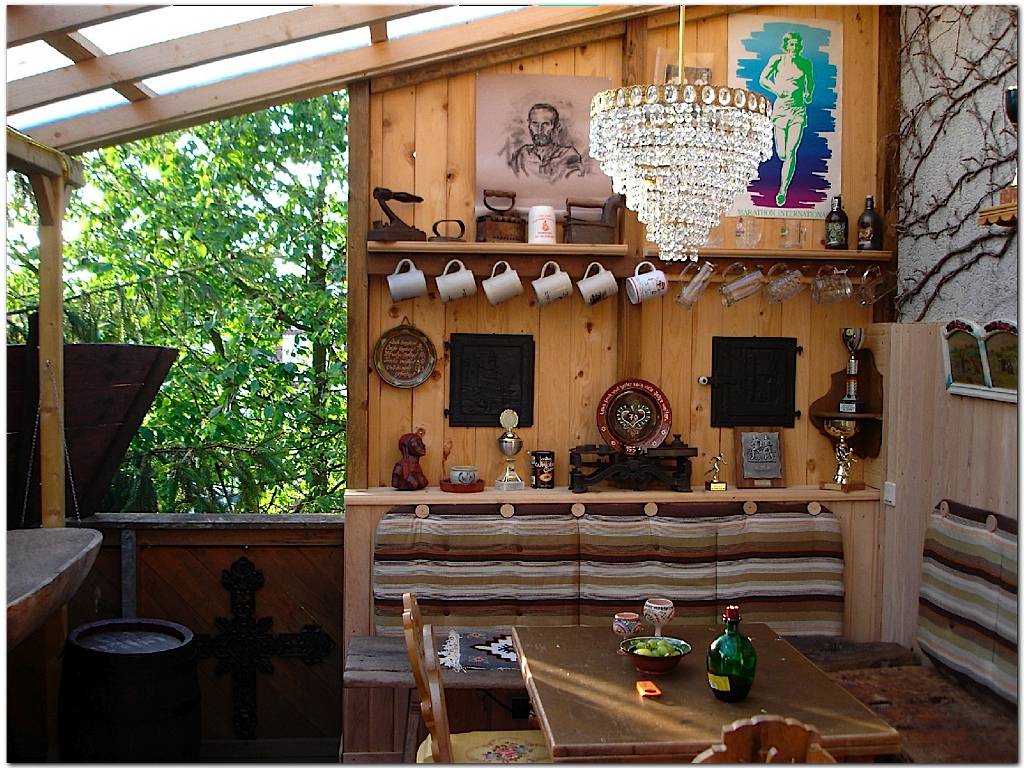
\includegraphics[width=300px]{images/DSC01605.JPG}\\
\textsc{Galer\'ia de la casa del maratonista.} \end{center}

Me di un ba\~no, orden\'e, y pens\'e en escribir en aquella mesita de afuera
pero ten\'ia hambre. Justo sal\'ian a la galer\'ia, as\'i que pregunt\'e por
una panader\'ia. En 500m me perd\'ia cuatro veces seg\'un su explicaci\'on,
as\'i que desist\'i de comprar pan terminando con las sabrosas barritas
energ\'eticas. Me invitaron a un vino, y charlamos sobre correr y el deporte.
Contaban que la galer\'ia era nueva, para festejar su cumplea\~nos en 12
d\'ias.

\subparagraph{}\label{ssub:queEdadTenes} --- Cuarenta. -- dijo el amigo.\\ ---
Gran fiesta -- contest\'e sin saber por qu\'e, y se re\'ian.\\ --- Sesenta y
cinco -- corrigi\'o el deportista.\\ \hangindent=1cm

\textexclamdown Sesenta-y-cinco a\~nos! Lo miraba sorprendido.

Me explic\'o el significado de algunos adornos: una cuna con interior de metal
serv\'ia para enfriar las cervezas en la fiesta, y tambi\'en para mecer a
alguno de sus tres nietos en la vida cotidiana. Un balde de lata atornillado a
un largo palo serv\'ia, me hizo entender, para orinar, \textexclamdown y
tirar los desechos de un garrotazo hacia afuera! ``\textexclamdown Esta noche lo
usar\'e!'', y risas.

El amigo sali\'o al atardecer, se nos complicaba la comunicaci\'on pero no
terminaba. Desde abajo llam\'o, el hombre. No se qu\'e le dijo en alem\'an al
due\~no de casa, y le tir\'o una bolsa con suficientes sobras de ese pan con
semillas. Me lo dejaba para que comiera antes de dormir, \textexclamdown as\'i
de hambriento me habr\'a visto! Ahora me mostraba trofeos, y al ver mi inter\'es
trajo \'albumes con fotos y recortes de diarios. Como le dije que me gustaba tal
foto y tal remera, me las regal\'o. La foto se hizo postal y ten\'ia copias; la
remera era de una competencia de la que le habr\'an quedado varias, no tan
lindas pero \'utiles. \textexclamdown Si me vieran vestido me entender\'ian!
Entre las notas que me impresionaron: varios recortes para los diferentes ``6
d\'ias de Francia'' mostrando c\'omo escalaba posiciones en cada a\~no hasta
llegar a correr (corriendo/durmiendo, de eso se trata esta competencia) 550~km.
En 3 d\'ias, 325~km. En 24 horas \emph{non-stop}, 225~km. Es decir que
exactamente en 24 horas llegar\'ia a Buenos Aires trotando, no m\'as, como un
caballo. R\'ecords para Alemania y casi para el mundo. Claro, de quienes se les
ocurre hacer esto, \textquestiondown cu\'antos llegan? Un d\'ia sali\'o de su
pueblo del centro alem\'an, y lleg\'o a la costa atl\'antica de Francia, un
pueblo precioso. Sus fotos tan barbudo me recordaron a ``Forrest Gump''. Anduvo
una semana por el Sahara. \textquestiondown Ahora ven c\'omo no es tan loco
viajar en bici? \textexclamdown Siempre hay uno que est\'a peor! O con m\'as
agallas.

Ahora a acostarme en la calentita cama (por fin, despu\'es de otros
80~km). Ma\~nana me despierta con el desayuno, y sigo viaje. \textexclamdown
Otro d\'ia ``kinder''! No parece, como tantos otros, un solo d\'ia.
\textexclamdown Esta ma\~nana sal\'i desde Kassel!

\textexclamdown Beso grande a todos!

Tute.

\subsection*{S\'abado 27 -- Marburg (esta vez s\'i)}

Me levant\'e a las 8 con las campanadas de una iglesia en Treysa, a 4~km de
Schwalmstadt. Ducha y lectura, Bernd me llam\'o luego a desayunar en
otra sala. Aqu\'i era (como en el resto de la casa, pero acentuado) todo de
madera o barro, muy natural, un toque oriental. Este hombre, descubr\'i
despu\'es, hace acupuntura y masajes en los pies. \textexclamdown El enfermo
corre descalzo! ``\emph{The best}'', dice. Incre\'ible. Y otro comentario que
me olvid\'e: las carreras de larga duraci\'on eran en c\'irculos de 400 m.
\textexclamdown Qu\'e aburrido! Hasta se cansar\'ian m\'as los m\'usculos de
un costado, los que doblan.

Hizo una ensalada en un pote de barro decorado; ten\'ia manzanas, duraznos,
bananas, frutos secos, algunas pasas, y ese queso blanco. Riqu\'isima y muy
nutritiva. Hab\'ia tambi\'en, entre las cosas t\'ipicas de un desayuno, salame
y bastante pan y queso. Una frutera con 4 o 5 manzanas que estar\'ia de
adorno. \textexclamdown Y el t\'e, sin leche! Mirando afuera a la copa de los
\'arboles termin\'e mi desayuno, entonces envolvi\'o todas las sobras y me las
regal\'o para el viaje. No creo que haya visto en mi cuaderno que estuve
aprendiendo c\'omo decir en alem\'an ``d\'onde compro frutas'' para antes de
salir; le peg\'o en el clavo con el buen regalo.

Me mostr\'o luego notas de diarios sobre el cruce de Alemania corriendo, y
luego se ofreci\'o a hacer de gu\'ia por la ciudad, antes de mi viaje.
Acept\'e y salimos a caminar. Recorrimos el casco antiguo, tom\'e un gran
caf\'e con leche en una plaza, escuch\'e hasta donde el entendimiento nos
permiti\'o sobre la historia de los lugares, y me impacient\'e de estar
sentado con el caf\'e, tan quietos, as\'i que volvimos a casa a buscar la
bici.

Tuve un lindo viaje, entre buen sol y viento. En menos tiempo del calculado
llegu\'e a la hermos\'isima Marburg, los mapas no ment\'ian al destacarlo.
Rserv'e dos noches en el hostal, pero me arrepent\'i y ahora escribo desde
Frankfurt. Hasta llegar al hostal hice diez kil\'ometros de m\'as, soy
especialista en alargar caminos aunque no quiera. Saliendo de Treysa hice
tambi\'en 5~km tomando una ciclo v\'ia que me escupi\'o, exactamente, al punto
de salida, \textexclamdown a la casa del maratonista! \textexclamdown Un rato
andando y volv\'i al mismo lugar! Qu\'e despiste.

Marburg es un pueblo colgado de las sierras, todas las casas son antiqu\'isimas
hechas con el mayor esmero y amor al detalle; y tiene una gran catedral y
castillo arriba. Llegu\'e a la hora de la siesta, y esa tarde no me mov\'i;
descans\'e y orden\'e la mochila (imposible no se porqu\'e). Al entrar en mi
habitaci\'on me di cuenta de que un compa\~nero dorm\'ia, despu\'es de hacer un
l\'io\ldots\ \textexclamdown lo despert\'e, pobre! Es que los horarios de esta
gente son raros. No salen pero salen, duermen hasta las 7am y de nuevo desde las
11am\ldots

Me ba\~n\'e, y le\'i un poco. Conoc\'i la \emph{Fachwerkstra\ss e}, ya recorr\'i
algunos pueblos sin saberlo. Me fui a un cyber, donde casi tres horas al
terminar de escribir me sorprendieron. De todos modos no me molest\'e porque
quer\'ia estar quieto, y lo lograr\'ia leyendo o escribiendo. Llam\'e a Gustav
saludando para el cumplea\~nos, y llegu\'e a mi casa temporal con ganas de bajar
el salame y los panes de Bernd. \textexclamdown Se me iba a complicar porque
comer solo era de mala persona, pero para invitar no me alcanzaba! Pensando en
c\'omo tratar el dilema entr\'e y vi a un solo joven: el que despert\'e al
llegar. Saqu\'e los panes, el salame y , gracias Ina por exigirme, la navajita
suiza.

Empec\'e a cortar sobre una silla pero marcaba la madera, as\'i que apoy\'e
sobre el cuaderno, que no se deshilach\'o mucho. Le ofrec\'i al chico, y
moqueando acept\'o s\'olo media rodaja con tres salames. Estaba medio triste,
vaya uno a saber porqu\'e. Fui a buscar agua, y empez\'o a charlar; me cost\'o
poco seguirle. Japon\'es, estudiante que habla poco alem\'an, y el Lunes le
dan una ``\emph{student Zimmer}'' para que se aloje. Imag\'inenlo hablando con
un argentino, que tambi\'en habla poco alem\'an, y el Lunes (pero Domingo, al
final) sigue viaje pedaleando. En estos hostales, en la mism\'isima habitaci\'on
y momento, se encuentran mundos tan incongruentes que hacen pensar en que no
existe s\'olo uno.

Nos comunicamos con se\~nas y algunas palabras. Incre\'ible hablar as\'i, pero
si no queda otra entonces se puede. \textexclamdown No saben lo argentino que
me sent\'ia cortando salame sobre un cuaderno sobre una silla, aunque con
navajita suiza! Agradeciendo el ofrecimiento (qu\'e bueno que no acept\'o
m\'as) sigui\'o viaje, y yo me ech\'e a dormir.

\subsection*{Domingo 28 -- Frankfurt {\small (ni m\'as ni menos)} -- 120~km en
5,5 hs.}

Durante la noche en Marburg, varias hormigas subieron por la pata de la cama,
y se instalaron en mi trasero. Baj\'e temprano (me despert\'o un reloj
prestado por el hostal), y llam\'e al bar de Mati, amigo m'io, para saludar en
la fiesta de cumplea\~nos de \'el y de Ezequiel (impresionante de nuevo, el
choque de mundos distintos: all\'a eran las 4am y estaban de buena joda).
Desayun\'e como ballenato luego de la migraci\'on, con vista a un campo de
deportes universitario bajo las verdes (y hoy soleadas) colinas.

Cuando abri\'o recepci\'on les coment\'e que me arrepent\'i de reservar dos
noches, y les pregunt\'e si pod\'ian devolverme el dinero para seguir viaje.
Lo hicieron sin problemas, y a las 9:30am estaba pedaleando.

\textexclamdown Por fin goc\'e de un suave viento a favor! Y entend\'i qu\'e
es lo que me mata: el parar y arrancar. Lo hab\'ia aprendido en el mal\'on que
me llev\'o de las pesta\~nas de Kassel, y hoy, un tipo que iba por mi senda,
m\'as adelante y a mi velocidad, sirvi\'o de zanahoria para este burro.
Hab\'ia tantas curvas que parec\'ia que me acercaba, pero
despu\'es manten\'iamos la misma misma distancia. Me entreten\'ia, y entonces
no baj\'e las velocidades en las curvas (\textexclamdown amo escuchar la rueda
delantera!) y empec\'e a andar un poqu\'in mas fuerte, se puede. Una vez
le\'ia sobre maratonistas: quien controla a la cabeza no es controlado por el
cuerpo, o algo as\'i. Si este loco no estaba ah\'i, seguro iba a 5 o 10~km/h
menos porque ``es mi velocidad''. Despu\'es de un rato lo alcanc\'e, pero
par\'e entonces a tomar agua: \textexclamdown era divertido! Pero el ciclista me
ven\'ia viendo y pensar\'ia: ``qu\'e hace este, que me adelanta sin
adelantarme''; baj\'o la velocidad y me qued\'e sin zanahoria. As\'i cubr\'i
30~km en 90 minutos casi, muy bien para m\'i. \textexclamdown De velocidad
s\'olo tengo los pelos desordenados, como ven!

Llegu\'e a Giessen, pueblo que deja bastante que desear trat\'andose de
Alemania. Es hermoso, pero uno viene con los humos altos para encontrarse con
algo ``simple''. Par\'e media hora y com\'i una bomba at\'omica envuelta en
masa de pan. Al darme agua, las panaderas no se sorprend\'ian tanto del viaje
en bici como del hecho de ser\ldots\ \textquestiondown argentino? Cada loco
con su tema. Y hablando de locos, as\'i me trae la falta de verduler\'ias.

Segu\'i a Friedberg, camino a Frankfurt. No se porqu\'e tenia marcado este
pueblo. Me sent\'i tonto: \textexclamdown me perd\'i tantas veces! En uno de
los pueblos que cruc\'e hab\'ia una banda t\'ipica tocando instrumentos de
viento, interesante y bello. Aprend\'i que me tengo que comprar mapas
detallados para \emph{todos} los lugares, y no s\'olo los que me interesan
particularmente. Recorr\'i 15~km de m\'as por lo menos. Despu\'es de un
enojado viaje y sin cosas interesantes (o que no supe apreciar) llegu\'e al
buscado Friedberg. El cartel que lo anunciaba era para m\'i todo un \'exito.
No se si estaba marcado por esto en mi hojita de viajes, pero tiene hermosas
construcciones, la m\'as vistosa es la belleza de gran torre que lo gobierna.
Faltaban 40~km para llegar a Frankfurt seg\'un una vieja poco informada de por
ah\'i, demasiado por el cansancio, aunque no tanto por la hora. Ah\'i el
hostal tiene nombre y apellido, mientras que antes no se d\'onde parar. Cuando
llegu\'e arriba de la torre se ve\'ian altos edificios a lo lejos al Sur, y
una placa indicaba que eran de Frankfurt, distante por ``escasos'' 24~km.
\textexclamdown Y se ve\'ian construcciones!

\textexclamdown Entonces llegar\'ia de un saque a Frankfurt! Fue bueno ver sus
torres, levant\'o los \'animos para seguirle dando sin pensar en la moribundez
que tra\'ia. S\'i, controlar la mente es lo m\'as importante. Descans\'e
tomando un helado en un banco de plaza. Estos descansos me encantan,
\textexclamdown soy tan croto, y todos se dan vuelta! \textexclamdown Algunos
se creen que hay que ser lindo para que lo miren, yo les mostrar\'ia este
contraejemplo! Me faltaba manchas de chocolate en la cara (por ah\'i ten\'ia)
para estar completo.

A 15~km de Frankfurt vi carteles a la vera de la ruta indicando que en los
alrededores de este pueblo que cruzaba no hay ``monstruosas'' turbinas
e\'olicas, diagramadas y tachadas como si fueran un pucho arrugado y humeante.
Se ve que no soy el \'unico loco, pero de todos modos me parece muy extremista.
\textexclamdown Lo que no voy a negar es que tuve un pac\'ifico y libre de
enemigos viaje!

La ruta se torn\'o autopista, y sub\'i a la bicisenda. \textexclamdown Ya
cumpl\'ia 110~km, y estaba bien! Supongo que durante el mismo viaje uno se va
entrenando y acostumbrando. Luego la confianza me jugar\'ia en contra, pero ya
llegaremos.

Frankfurt es inmensa, ni se por d\'onde entr\'e. Alg\'un lugar del norte.
\textexclamdown Para colmo ya encontraba un cartel que indicaba que sal\'ia de
la ciudad! ``\textexclamdown Qu\'e r\'apido la atraves\'e!'', pensaba. Volv\'i
a una estaci\'on de colectivos que ten\'ia mapa, justo llegaba la se\~nora con
el nene en bici que acababa de adelantar. \textexclamdown Y hablaban
espa\~nol! De Per\'u la se\~nora, viv\'ia hace unos a\~nos por ac\'a, y al
menos me supo se\~nalar en el mapa d\'onde est\'abamos, en el Noroeste de la
ciudad. Todav\'ia faltaba encontrar el hostal, \textexclamdown teniendo solo
la direcci\'on, hab\'ia tantas calles por leer en este detallado mapa! En
minutos lleg\'o otro hombre, acompa\~nado tambi\'en por el colectivo. La mujer
y el nene subieron. Empec\'e, un poco nervioso:

\subparagraph{}\label{ssub:habloEspanol} --- \emph{Sprechen Sie English?}\\
--- No, pero hablo espa\~nol. -- Contest\'o en tono alem\'an. Antes de que
subiera al bus le mostr\'e la direcci\'on. -- Sube al colectivo conmigo. --
Respondi\'o.\\ \hangindent=1cm

Sub\'i tan r\'apido que no se c\'omo entr\'o la bici. \textexclamdown Me
ca\'ia, y el nene mor\'ia de risa! Ten\'ia la mochila de un hombro, el agua en
una mano, el casco colgado de la bici sostenida por la otra mano\ldots\ Era un
payaso. \textexclamdown Y no sab\'ia a d\'onde iba ni con qui\'en!

El hombre era alem\'an, casado con una mujer de Rep\'ublica Dominicana. Nos
bajamos en una parada cercana a una estaci\'on de trenes, subimos a un tren.
Mientras me salvaba las papas (al menos eso quer\'ia creer en el momento, y
result\'o ser verdad) me contaba que asist\'ia a una gran fiesta latina en el
r\'io Main, a {\sl dos} cuadras de mi hostal. \textexclamdown Qu\'e buena
casualidad! M\'usica centro americana, y miles de personas. Yo lo miraba
extasiado pensando en c\'omo cornos encontr\'e al hombre que no conoc\'ia pero
que estaba buscando, y a la vez mor\'ia por mirar por la ventana del tren y
conocer en vez de escuchar la historia de c\'omo aprendi\'o espa\~nol en forma
autodidacta, y porqu\'e iba a esta fiesta tan cercana a mi destino. De todos
modos la ciudad no parec\'ia interesant\'isima en esta zona, y decid\'i
escucharlo; no tendr\'ia mucho m\'as tiempo para eso.

Bajamos del tren bajo tierra. Sub\'i dos pisos por escaleras con la bici.
\textexclamdown Peor, de cansador, que el mismo viaje! Y vi catedrales de lo
m\'as hermosas. Llegamos a lo que parece una plaza central rodeada de viejas
\emph{Fackwerkhauses}, y una detallada iglesia.

\subparagraph{}\label{ssub:Frankfurt} --- \textexclamdown Qu\'e hermoso!\\ ---
S\'i, \textexclamdown y no es viejo como parece! En la II Guerra Mundial, el
80\% de Frankfurt era escombros y cenizas, se reconstruy\'o siguiendo la
antigua l\'inea. Esas casas bien pueden tener tu edad.\\ \hangindent=1cm

Puta guerra. Hay monumentos en todos lados, contrario al preconcepto de tab\'u
que tra\'ia de all\'a. Incre\'ible todo esto nuevo, entonces lo cl\'asico y el
amor al detalle no se olvid\'o, como tambi\'en prejuiciaba.

Bajamos por una peatonal repleta de gente esperando. Era la cola para entrar al
puente peatonal colgante que cruza el r\'io. La fiesta es grande en serio. Ah'i
los peatones conservan su derecha. Hice malabares para poder subir y bajar la
bici. Cuando vi el r\'io desde arriba era una fiesta, y no s\'olo por lo latino.
Numerosas lanchas y barcos tur\'isticos surcando de aqu\'i para all\'a lo
tornaban alegre. Es hermos\'isimo, mientras escribo lo estoy viendo porque la
mesa est\'a bajo la ventana que da al r\'io. Me separan una calle (que sentado y
desde el segundo piso no veo) y el terrapl\'en. \textexclamdown Ni en un cinco
estrellas! S\'olo por pagar \geneuronarrow{15} por una habitaci\'on compartida.
Hay un olor a vino que mata: mis compa\~neros duermen.

El r\'io tiene 50m de ancho, \'arboles por las riberas, los que est\'an frente
m\'io color anaranjado oto\~nal; decenas de personas recorriendo los
terraplenes, y cientos en la fiesta, m\'as a la izquierda. Sol radiante, cielo
s\'olo interrumpido por la cantidad de rutas de aviones, que se multiplican
ac\'a, en la ciudad. Los aviones, que siempre se vieron en lo alto, ahora
descienden. Los edificios tambi\'en decoran. \textexclamdown Si no ca\'i en lo
m\'as lindo de Frankfurt es de las ciudades m\'as hermosas, sin dudas! Me
record\'o mucho a Chile todo. La ruta por estar viajando entre colinas con autos
``raros'' por un pa\'is desconocido, y Frankfurt porque, siendo tambi\'en bella,
es desordenada (aunque no tanto) como Santiago.\\

Al bajar del puente desped\'i a mi \'angel de la guarda (se llama {\sl Gunther}). 'El fue para el lado de la fiesta, yo las dos cuadras para el
otro. Cinco en realidad, por un polic\'ia que en vez de contestar ``no s\'e''
me mand\'o para otro lado. Me hartan. \textexclamdown Tras que tengo la
br\'ujula ah\'i donde me pican las hormigas!

Feliz de la vida de completar tan bien del cuerpo semejante etapa. Al llegar
cen\'e buenos alimentos en el hostal, me sorprendi\'o de nuevo lo barato. Una
ensalada de arvejas, choclos y zanahorias hervidas, aunque les suene raro, fue
un manjar. \textquestiondown Saben qu\'e? Esos caramelos de oficina que
ofrecen en los mostradores son una gloria. \textexclamdown Por fin estoy
viajando con hambre irracional! Es parte del viaje.

\textexclamdown Y ahora estoy archivando mi mapa del centro de Alemania para
sacar el del Sur! Estoy a 90 km de Heidelberg pero por m\'as hormigueros que
me ataquen ma\~nana no lo voy a hacer. Si el cagac\'in me lo permite (``plata
y pasaporte siempre con vos'', indic\'o el de recepci\'on) ma\~nana pasear\'e
por esta gran ciudad alemana. Si no lo hago, de todos modos tengo varios
hostales antes de Heidelberg.

\textexclamdown Gracias por todos sus mails!

Tute.

PD: Acaba de entrar una se\~nora en una bici peque\~na; de una patada mand\'o
la rueda trasera (chica como la delantera) bajo el asiento. Casi no ocupa
lugar. Estoy conociendo buenos artilugios cicl\'isticos.

\subsection*{Lunes 29 -- Heidelberg -- 30~km en bici, otro poco en tren}

\textexclamdown Hola a todos! Muchas gracias por sus mails, leo todos y
agradezco. \textexclamdown Pero sepan que no contesto a todos por rata! Vean,
hoy me siento estafado por cada m\'aquina que toqu\'e. Llegu\'e al hostal de
Karlsruhe y una compu que funciona a monedas (\textexclamdown cara encima!) me
trag\'o \geneuronarrow{1}. Fue el m\'as llorado de todos mis gastos. Puse otro,
se termin\'o r\'apido. Llam\'e a lo de Gustavo y me comi\'o 10 centavos,
adem\'as de no aceptar tres monedas de 20. Me atendi\'o el contestador\ldots\ El
cyber es por cuenta regresiva, estoy a las apuradas. As\'i que as\'i se vive:
\textexclamdown hoy me levant\'e con la pata izquierda para la computaci\'on!
Pero al cenar, o me confundieron con un contingente de viajeros o era
inclu\'ido. Cr\'edito para las comunicaciones.

Empiezo desde la ma\~nana Frankfurteana. Me despert\'o un ``compa''
japon\'es, le ped\'i que lo hiciera para llegar al desayuno. Me levant\'e
mientras el muchacho hablaba con el otro hospedado, un norteamericano que
ven\'ia de Kuwait. Estuvo al servicio de una compa\~n\'ia de Ingenieros como
mec\'anico. Interesant\'isimo. El que me despert\'o miraba con los ojos grandes;
\textexclamdown no parec\'ia japon\'es! Aunque por ah\'i era porque no
entend\'ia un pomo: se le complica con el ingl\'es y sin embargo charlaba,
hasta se sac\'o una foto conmigo al irnos.

Desayun\'e demasiado, \textexclamdown primera vez que me siento ``gordo'' a las
8 am! Segu\'i viaje despu\'es de una corta caminata por Frankfurt. Ya veo lo que
me perd\'i al leer sus mails, en la ansiedad y poco de cagazo del momento
prefer\'i seguir. Como las noches en Chile, no se porqu\'e me pongo inquieto y
ya no disfruto mirando las cosas. Algo que quiero cambiar. La falta de
informaci\'on fue letal para este paseo urbano, veo que es ley visitar
informaci\'on tur\'istica. La peque\~na caminata bonita, recorriendo los lugares
que no pude ver por la presencia de incontables personas el d\'ia anterior.

Sal\'i hacia el sur, las piernas ayer no molestaron pero se guardaron todas
las quejas para hoy. Aunque lo que m\'as molestaba era el traste; ya compr\'e
el\'asticos que sujetan la mochila a la bici. La gota que rebals\'o el vaso:
20~km en direcci\'on equivocada, \textexclamdown nunca m\'as en bici sin mapas
detallados! As\'i que festejen: mi orgullo cedi\'o ante el enojo. Tom\'e tren a
Heidelberg, distante por 90~km. (En los 20~km equivocados pas\'e por un estadio
en remodelaci\'on para el mundial 2006.) Traspaso estresante (se iba el tren
mientras bajaba con equipaje y bici por escaleras mec\'anicas) llegu\'e a la
estaci\'on de Heidelberg en el siguiente. Combin\'e con un trencito desde el
estadio hasta el aeropuerto de Frankfurt, \textexclamdown es inmenso! Con la
bici de ac\'a para all\'a por todo el aeropuerto comprando pasajes, preguntando
si es pasaje con bici, qu\'e hago si perd\'i el primer tren\ldots\ Combinaci\'on
en ``Frankfurt Main'', la estaci\'on principal, \textexclamdown y a Heidelberg!

No muy hospitalarios en informaci\'on tur\'istica, me informaron el camino que
necesitaba, y llegu\'e a mi hostel atendido por un no hospitalario joven.
Habl\'abamos en tono normal, pero con tanta iron\'ia que la adrenalina se
hac\'ia sentir; nos juntamos dos con los cables pelados. La zona del hostel no
es linda, as\'i que este d\'ia no pintaba fascinante, pero dej\'e bolsos y bici
y encar\'e para la zona antigua y castillo.

\subparagraph{}\label{ssub:Heidelberg} --- \textquestiondown Queda lejos para
ir a pie?\\ --- S\'i, para ir a pie es bastante lejos.\\ \hangindent=1cm

\textexclamdown No se para qu\'e pregunt\'e, si igual no me subir'ia a la
bici por nada!\\

Empieza justito aqu\'i el viaje tur\'istico, y no viaje ``viaje''. Paisaje
m\'as tupido, construcciones m\'as mantenidas, vasos ornamentales de 1l
alemanes por todos lados (c\'omo me gustan), mucha gente, dos m\'usicos con
flauta dulce y bandone\'on tocando alegres valsecitos en la peatonal, un
cantor con guitarra haciendo m\'usica divertida tipo folk en la cuadra
siguiente, callecitas angostas, enormes iglesias, una helader\'ia por cuadra.
Se empieza a nombrar la Selva Negra. Entr\'e en un cyber a leer mails, y
termin\'e de levantar la cabeza. Conoc\'i el viejo y gran castillo, desde donde
se tiene una gran vista a Heidelberg y su r\'io. Camin\'e mucho la verdad, y
cre\'ia que por ah\'i el d\'ia de descanso no lo era tanto. Pero la caminata no
molest\'o para el pedaleo. Dicen que hab\'ia 9~km hasta el castillo.

\textexclamdown Escuch\'e de nuevo el avi\'on caza! Me alej\'e de edificios y
levant\'e la vista. En 5 segundos pasaba por sobre nosotros y lo ve\'ia
doblando r\'apido como doblan esos aviones, color oscuro era. En otros 5
segundos desaparec\'ia. Claro, al no ir tan alto uno ve la tremenda velocidad
a la que avanzan. Me sorprendi\'o un mont\'on, esos bichos son tan
incre\'ibles como los aviones grandes. Mucho m\'as, por c\'omo se mueven.

Volv\'i caminando por el r\'io, por el lado de un verde parque lleno de gente
al sol. Bien alimentado (hoy no me priv\'e de ning\'un gusto), descans\'e bien.

\subsection*{Lunes 30 de Agosto -- Karlsruhe -- 80~km}

(Casi pierdo el mail que acabo de escribir y prendo fuego el cyber.)

Hoy me levant\'e y desayun\'e bien. \textexclamdown Qu\'e bueno no
extra\~narlo! Eso s\'i, no mencionar lo que extra\~no unas ``Melbas'' en la
tarde porque me tomo un avi\'on. Pregunt\'e a cuanta persona se me cruz\'o por
el camino de salida de Heidelberg y entonces no me perd\'i gravemente, s\'olo
una vez. \textexclamdown Ya voy a llegar a Strassbourg, desde donde empieza mi
detallado mapa de la Selva Negra! Marca hasta las bocas de tormenta de las
calles.

En el largo camino, los diferentes pueblitos fueron la estrella, todav\'ia no
empiezan cosas muy diferentes a los alrededores de G\"ottingen. Incluso no tan
bello como en esas tierras, por menos \emph{fachwerkhauses} y mayor tama\~no.
Llegu\'e a Karlsruhe, una ciudad grande y bonita en donde par\'e obligado a
descansar, en un intento por implementar el no andar hasta matarme.

Ma\~nana al mediod\'ia llego a Baden-Baden, donde, luego de recorrer, dormir\'e.
De Francia me distancian alrededor de 105~km, que completar\'e en dos d\'ias.

\textexclamdown Por fin encontr\'e una verduler\'ia! El alem\'an hablaba
espa\~nol, me indic\'o que el nombre de las zanahorias es ``\emph{carroten}''.
Compr\'e varias \emph{carrotens}, y otras tantas \emph{bananens}, que com\'i
r\'apido porque no sab\'ia c\'omo amarrarlas a la bici sin hacerlas pur\'e. Me
regal\'o una manzana: ``\textquestiondown Necesitas combustible?'' La com\'i
tres horas despu\'es, y estaba tan sabrosa que me arrepent\'i de no haber
llevado otras m\'as.

Vengo del castillo de Karlsruhe, es muy lindo, grande aunque no alto, color
amarillo y bastante nuevo parece. Tiene un parque grande, prolijo y con lagos;
es una belleza.

Gracias por sus mails, por aqu\'i todo m\'as que bien. Ahora a dormir, y
ma\~nana a desayunar para seguir viaje. \textexclamdown Qu\'e vida rutinaria
me toca! Beso grande a todos;

Tute.

\subsection*{Martes 31 -- Baden-Baden -- 60~km}

\textexclamdown Hola hola, familia y amigos! \textquestiondown C\'omo andan,
todos? Yo aqu\'i muy bien y contento. Hoy tuve un d\'ia relativamente
tranquilo, y conoc\'i mucho.

Me levant\'e temprano, desayun\'e bien. C\'omo me gustan los cereales con
leche, coca-cola y helados\ldots\ ya estoy empezando a tener esa mentalidad
hermosa de viajar en bici, de desear locamente cosas cotidianas.

Empec\'e viaje cruzando hacia el sur Karlsruhe, y, entre idas y venidas, me
pas\'o un loco en bici. Paramos en un cruce, y le pregunt\'e por Ettlingen. Me
indic\'o y pregunt\'o a d\'onde iba, o qu\'e hac\'ia en esa ciudad. Le dije
que sigo hacia Baden-Baden y expliqu\'e a grandes rasgos el viaje. ``Bueno,
vamos juntos porque yo voy para all\'a''. El tipo rozaba los 30, charlamos un
buen rato e hizo que se me esfumaran 15~km del camino. Entre lo interesante,
hablando sobre los soldados franceses que dejaron hace poco Baden-Baden, y una
confusi\'on m\'ia sobre aliados y enemigos, dijo:

\subparagraph{}\label{ssub:FranciaAliada} --- Francia no estaba aliada con
Alemania, como todo el mundo. Y ten\'ian razones para no estarlo.\\
\hangindent=1cm

Algo claro como que uno se quema con el fuego, pero al escucharlo de un
alem\'an se recibe con m\'as peso. Adem\'as, por c\'omo lo dijo parec\'ia
estar arrepentido de su propio pasado; es todo tan duro. Como dice Gustavo,
que los j\'ovenes pagan el pato por lo que hicieron generaciones anteriores.

A 10~km de Baden-Baden volvi\'o a Karlsruhe porque el d\'ia anterior hab\'ia
hecho no se que raid. Me met\'i en bosques, y me perd\'i. Es que estaba en la
Selva Negra y los caminos eran aburridos, \textexclamdown prefiero perderme
por bosques! Muchas construcciones. Al llegar a Baden-Baden com\'i
sanguchines, tienen unas verduras raras para m\'i, muy ricas. Es una ciudad
alargada y al final est\'a ``lo bueno'', as\'i que al principio me pas\'o lo
mismo que en Heidelberg.

Llegu\'e a mi hostel (al lado de un club con pileta, el caluroso d\'ia me
hac\'ia dudar) y dej\'e todo porque todav\'ia no estaba el recepcionista. Fui
a pie al centro, camin\'e un mont\'on conociendo. \textquestiondown Saben
c\'omo lo comparo, para que se den una idea? Con todo el sabor de estar en
otro continente, pero es como si seleccionaran todos los edificios m\'as
lindos y viejos de nuestra Capital, y los instalaran ac\'a. Porque no denotan
extrema antig\"uedad, o estilo puramente alem\'an. Son con balconcitos con
rejas, no son de estilo \emph{fachwerk}. Me contaba mi ``compa'' ciclista que
ac\'a est\'a la clase m\'as alta, y se nota en autos, comercios, y el estilo del
centro. Cruza este pueblo un cursito de agua rodeado de vegetaci\'on. Un lindo
lugar, pero no me me\'e como esperaba. Justamente por eso: esperaba demasiado.

Camin\'e a los castillos. Saqu\'e mil fotos, porque me separaba del castillo
viejo una caminata de 4~km, en subida en curvas y por los densos bosques. Las
mosquitas se me met\'ian hasta en las orejas. En los ojos no molestaban porque
ya me traen de hijo las moscas de la ruta, y si bien grito de furia ya me
acostumbraron. El castillo viejo parece ser de los a\~nos 1400,
interesant\'isimo y alt\'isimo. La visibilidad no era 100\% hoy a pesar del
gran sol, pero lo que m\'as me gusta de visitar estas antig\"uedades es,
despu\'es de la cantidad de pasadizos y enormidad de lugares que contienen, la
gran vista hacia abajo, a cualquier punto de los 360$^{\circ}$. Ah\'i s\'i que
los reyes se sienten reyes.

La mujer de info tur\'istica me dijo que Baden-Baden es famosa, entre otras
cosas, por su casino. 19 a\~nos y pinta de bicicletero (con manchas de aceite
en pantorrillas atestiguando) hicieron que ni dudara de querer pasar. Las
termas deben ser incre\'ibles, debe ser un lugar para meterse un d\'ia y
quedarse una semana quieto (por eso mismo es que no voy). Entr\'e en un
lugar muy lindo, \emph{festspielhaus}. Cuando lo relea sabiendo m\'as, o
cuando lo lean quienes saben, se quejar\'an de esta descripci\'on, pero por
cantidad de detalles y hermosura en cada rinc\'on lo comparo con el Teatro
Col\'on.

Sabore\'e un helado sentado en un banco de plaza en una peatonal, bajo estos
edificios que en cada ventana tienen flores. Mientras, miraba mi
remera, no se si llevarla a la fiesta del color o usarla para
el carnaval carioca del casamiento de mi hermano en Pergamino. \textexclamdown
Pensar que hubo un tiempo que ten\'ia s\'olo tres colores, contando el logo!
Hoy la decor\'e con un poco de rosa tambi\'en, por un fruto que parec\'ia rico
de un \'arbol, pero que era m\'as agrio que un lim\'on. \textexclamdown Es
c\'omodo mi repasador! Uso todos los d\'ias la misma, y para dormir tambi\'en
pero otra. Traje 4 remeras y no se para qu\'e. Las lavo en la ducha y las seco
durante la noche.

Compr\'e un libro, termin\'e el anterior. No me queda otra que leer en los
verdaderos descansos en el hostal. Lo que s\'i: no s\'e que cornos hacer con
el anterior, porque no me interesa tanto como para llevarlo por todo el viaje,
y la mochila est\'a abultada como para encajarla en el portaequipajes. Ya
encontrar\'e soluci\'on, esta biblioteca lo revend\'ia si parec\'ia nuevo.
Pero parece sacado de un tesoro pirata hundido.

Ya se ven monta\~nas que prometen cansarme pero tambi\'en entretenerme. Ahora
saboreo otro helado y al hostal, a dormir para ma\~nana seguir. Estoy a 60~km
de Estrasburgo, as\'i que si no me pierdo m\'as de tres veces llego en el
d\'ia a Francia. Aunque con mi mapa detallado ahora las probabilidades de
perderme decrecen. \textexclamdown Era hora!

\textexclamdown Gracias por todo, no saben lo cerca que me hacen sentirlos a
pesar de lo lejos que estamos! Estoy oliendo pat\'e y es la primera vez que
deseo uno desde el primer viaje al Sur. \textexclamdown Beso grande a todos!

Tute.

\subsection*{Jueves 1 de Septiembre -- Stra\ss bourg -- 104~km en 5:40 hs.}

\textexclamdown Hola hola, familia y amigos! Qu\'e rompe quinoto estos
franceses, metieron su teclado en una licuadora y sali\'o todo mezclado.
\textexclamdown Vean que me cruc\'e hasta la lejana Alemania para poder
escribir! La necesidad de comunicarme en realidad.

El gran d\'ia empez\'o en Baden-Baden. Si bien no hab\'ia quien me despertara
(\textexclamdown habitaci\'on para mi solo! Como ac\'a en Francia) me
levant\'e a las 7:32, casi como reloj cuc\'u. Casi, porque hac\'ia ya como dos
minutos que hab\'ia abierto la cafeter\'ia. No puedo dormir m\'as de ocho
horas, siendo que el deporte regula todo lo atribuyo a eso. Me dorm\'i ayer
leyendo ``The Zahir'', de Coelho, me gusta como escribe.

Luego de desayunar me agarr\'o la locura repentina, y saqu\'e cosas
irrelevantes de mi mochila; se ca\'ian del portaequipajes. Volaron una remera
``linda'', el libro le\'ido, vasos alemanes prometidos para los amigos, y otras
chucher\'ias que vi que no usar\'ia. Encar\'e para el ``trocen'', y dej\'e todo
en la oficina postal para Gustav. Qu\'e comodidad, ahora.

Una mujer me indic\'o el camino que quer\'ia, pero cre\'i que en sentido
contrario. Volv\'i a info tur\'istica a comprobar y era correcto lo que ella
dec\'ia. He aqu\'i los eternos 10~km adicionales. En info me quer\'ian indicar
una ruta directa a Francia, pero por la parte amarilla del mapa. Yo quer\'ia
la que se ve sin un mil\'imetro recto.

\subparagraph{}\label{ssub:Subida} --- \textexclamdown Pero es todo de subida!
-- Informaron.\\ --- \textquestiondown Pero por bosques?\\ --- S\'i, por los
bosques.\\ --- Bueno, \textexclamdown eso es lo que quiero!\\ \hangindent=1cm

Despu\'es comprob\'e que no ment\'ia. Cuando rechac\'e su carretera pusieron
cara de ``'este se cree H\'ercules'' (me captaron tal como
soy) as\'i que pens\'e que dormir\'ia a mitad de camino: Achern. Pas\'e por
una panader\'ia para comprar energ\'ia compactada en masa de pan (juro que le
hice elegir lo m\'as suculento al buen muchacho) y empec\'e de ma\~nana mi
sereno viaje.

Sal\'i de Baden-Baden por el otro lado del que entr\'e. Sal\'i por la senda que
bordea al peque\~no curso de agua, que suena serenamente al bajar los
escaloncitos. Alrededor, pasto perfecto, y cruzan puentes de colores, de hierro
trabajado o madera, llenos de esas florcitas que abundan decorando Alemania.
Viendo un descampado not\'e que ni siquiera se escuchan los autos. Tangible paz.
Todo rodeado de suaves cerros cubiertos por \'arboles.

Llegu\'e a la ``famosa'' ruta 500, ``\emph{Schwarzwald Hochstra\ss e}'', y, en
la velocidad en que se avanza poco m\'as que caminando, empec\'e a subir,
tranquilo y observando. Me iba separando de la ciudad para ver que se
convert\'ia en un lejano valle, con casas perdidas y el pasto salpicado de
dientes de le\'on. Esto cuando los \'arboles permit\'ian a mi vista alejarse,
de otro modo todo lo que se ve es un t\'unel de cerrada vegetaci\'on. De a
poquito me fui metiendo entre sierras y monta\~nas bajas, y por fin lo sent\'i
y cre\'i: estoy en la Selva Negra. Lo que describ\'i es eso, la primera vez
que lo siento. Me acord\'e tambi\'en de que lo que m\'as me importa en los
viajes es que el camino sea lindo, no el lugar a donde llegar. Si no, empiezo
a calcular cu\'anto faltar\'a y me canso irremediablemente. Pero as\'i me
importa un r\'abano siquiera a donde voy, si estar en ese camino es el
mism\'isimo placer que busco.

Si bien el mapa indicaba bicisenda, la ruta estaba rodeada por acantilado o
monta\~nas de densos bosques; no quedaba espacio para un camino paralelo.
Entonces, cuando vi un cartel para bicis me met\'i de repente, siempre es
mejor que con autos. El camino era de ripio y segu\'ia en bajada.

Bajaba frenando por miedo, no pas\'e los 40~km/h creo. \textexclamdown La
bajada en curvas ten\'ia interesante pendiente! La suspensi\'on dura repet\'ia
las piedras en mis manos, me asustaba un poco perder el control. Se ve\'ia en
un valle un pueblo y casas t\'ipicas perdidas, de esas con techo ``a tres
aguas''. Era raro el pueblo, con calles en pendiente, largas y sin bocacalles,
que al doblar giran 180$^{\circ}$, y con casas entre medio que sospecho
tendr\'an escaleras para comunicarse entre s\'i. Tienen un modo particular de
nombrar las calles y lugares, obvio diferente a nuestros perpendiculares
carteles numerados. Bajando y bajando un poco m\'as llegu\'e a B\"uhlertal. Me
fij\'e en mi s\'uper-mapa (justo ah\'i empieza) y vi que (por supuesto) me
hab\'ia desviado, pero de la idea y no del camino a Francia. Corrobor\'e la
forma de la ciudad en el mapa, tiene calles realmente intrincadas. Pueblo
entre los cerros que cuando no tienen selva tienen cultivos frutales (tan
prolijitos como en Chile), tantas casitas bonitas, tranquilidad y belleza
natural. Saqu\'e varias fotos. Tenia miedo de tener que volver a subir a ``la
500'', pero baj\'o por otros lugares supongo. Com\'i el segundo pan (el
primero fue en el camino porque los el\'asticos rasgaban la bolsa, el tercero
mientras escribo y engraso la lapicera) y segu\'i viaje a Achern, donde
dormir\'ia.

Llegu\'e a las 14hs, con 50~km recorridos y fresco como una lechuga. Claro, la
subida fue con toda mi paz, y en la bajada no pedaleaba. En el fondo empezaba
a amenazar la tormenta prevista para hoy, aunque me levant\'e con sol radiante
que me acompa\~n\'o hasta aqu\'i.

Fren\'e para ver mapas mientras pensaba si seguir, era temprano. No sab\'ia
por d\'onde exactamente, as\'i que le pregunt\'e a una italiana que andaba por
ah\'i: ``\emph{Sprechen Sie English?}'' Murmur\'o algo acompa\~nado de
``\emph{parlo}'', supuse que no hablaba ni alem\'an ni ingl\'es. Pasaba otra
se\~nora y me ech\'o la mirada de ``\textquestiondown Necesit\'as ayuda?'' Yo
le di la mirada de ``S\'i, se\~nora, necesito urgentemente su ayuda'', as\'i
que se sent\'o a mi lado. Me dijo que Estrasburgo estar\'ia a 30~km (mucho
menos de lo que pensaba, aunque ser\'ia un poquito m\'as), marc\'o el mejor
camino a seguir ya que no hay rutas directas, y me indic\'o que llegar\'ia
antes de la tormenta, que se largaba en dos o tres horas. Con gestos me
indicaba que se ven\'ia con rayos:

\subparagraph{}\label{ssub:Tormenta} \emph{--- Raining?\\ --- No.\\ ---
Lightning?\\ --- Yes, lightning!}\\ \hangindent=1cm

Fue como una palmada en el traste, segu\'i con todo. Como nuevo y bien comido,
complet\'e 20 o 30~km a buen promedio, mientras las nubes iban tragando las
monta\~nas que dejaba atr\'as. Pas\'e por frutales y com\'i ciruelas y
manzanas, no solo de pan vive el hombre. Le pregunt\'e a un hombre que
descansaba en su auto si pod\'ia seguir por la ruta (creyendo que se
convertir\'ia en autopista) y me dijo que s\'i, que ``el puente del Rin es
para todo tr\'afico''. Interesado y de buena gana me hizo algunas preguntas y
me dej\'o seguir.

Fue el hombre que m\'as pute\'e. S\'i, se transformaba en autopista. Me
estreso en las autopistas m\'as que en un tornado, adem\'as de la inseguridad
s\'e que es ilegal para bicicletas. A los 400 metros, cuando me asegur\'e de
que no habr\'ia salida, volv\'i a pie entre el guardariel y un alambrado. Los
arbustos de la banquinita me iban arrinconando, hasta que me llenaron de
bichos y telas de ara\~na. Lo que me puso loco metros antes de llegar a un
puente donde subir\'ia: esas ortigas que pican y arden toc\'andome las
piernas. Furioso me acerqu\'e por el asfalto hasta el puente, escuch\'e un
justificado y no cercano bocinazo, y cruc\'e de nuevo el guardariel. Tir\'e la
bici por arriba del alambrado, despu\'es yo. Sub\'i el puente (me patinaba
hacia abajo) y a\'un restaba un metro de cemento en vertical para llegar al
camino que cruzaba. No hab\'ia otra salida por los densos bosques.
Trep\'e, y arrastr\'e hasta arriba la bici, tomada del manubrio. Transpiraba
caudalosamente, y ya no me quedaba agua; com\'ia ciruelas, almacenadas como
buena ardilla.

El cuento tiene final feliz, porque encontr\'e una ciclo v\'ia internacional,
as\'i que estaba marcada como para tontos, \textexclamdown exactamente como
necesito! Hice una excepci\'on y tom\'e un helado antes de la llegada (a
calmarme un poco), donde adem\'as cargu\'e agua fresca. En todo el l\'io me
olvid\'e de la tormenta, que se ve no se anim\'o a seguirme hasta Francia,
as\'i que recorr\'i los \'ultimos 10~km de nuevo tranquilo. Pas\'e por aqu\'i
a una pareja con unas alforjas que son mi envidia: la misma forma que las
m\'ias argentinas (la mejor) pero dividida en tres bolsos de tapa dura para
usarlas en cualquier momento de modo c\'omodo.

La \'ultima ciudad alemana, Kehl, me recordaba, aunque en la urbanizaci\'on e
infraestructura alemana, a la paz, tranquilidad y orden de las calles de Punta
del Este (fuera del verano). Al menos el barrio cercano al r\'io, es ciudad
grande y seguro no la conozco toda. Llegu\'e al Rin (no se porqu\'e me
descoloc\'o que corriera hacia el Norte) y lo cruc\'e por un puente peatonal
colgante admirable para Ingenieros como para dise\~nadores. No tiene nada recto.
Las dos columnas est\'an ``chanfles'' sosteniendo con tirantes diagonales a dos
tramos curvos (pedestre y para ciclistas). Entre medio de los dos caminos hab'ia
vigas que los un\'ian. Invita a estudiar est\'atica.

Llegu\'e tipo 4 pm, y fui seg\'un un mapa a informaci'on tur\'istica, donde
encontr\'e un desprolijo descampado. Pregunt\'e a un hombre, y en alem\'an me
explicaba pero no pod\'ia entenderle. A lo \'ultimo:

\subparagraph{}\label{ssub:estaAhi} --- \textquestiondown Pero vas al hostal
juvenil vos? \textexclamdown Si esta ah\'i!\\ \hangindent=1cm

Lo se\~nalaba con la mano. Incre\'ible. No me met\'i en la ciudad: a orillas
del Rin dormir\'ia. Saqu\'e dos noches para descansar y conocer tranqui. Llam\'e
por tel\'efono por el dilema de los teclados. (\textexclamdown No puedo ni
tipear mi nombre para entrar a leer mails, casi!) \textexclamdown Y tienen hasta
lavander\'ia! Probablemente la use. (Al final continu\'e con mi costumbre,
\textexclamdown y no lo hice!) Contento, luego de muchos kil\'ometros y bien
recorridos.

No saben qu\'e bueno es escuchar un idioma al que no le cazo ni el ``hola''.
Hace sentir el viaje a lo nuevo m\'as lejano e interesante. Es incre\'ible lo
diferente que uno siente las mismas cosas pero en otro pa\'is. Me sent\'e en
el parque del Rin mirando hacia Alemania, y sent\'ia que estaba haciendo algo
incre\'ible, aunque solo respiraba mirando; ni siquiera abr\'i el libro con
esa sensaci\'on de ``incre\'ible\ldots''. En Alemania me siento m\'as como en
casa, con familia y casa donde vivir y conociendo cada vez m\'as; pero salir
del pa\'is es hermoso. Aunque en los minim\'isimos detalles, todo es
diferente.

Al atardecer sal\'i a caminar. Primero a la plaza cerca del puente, hay dos
monumentos dedicados a la recuperaci\'on de Alsacia. Luego encar\'e al centro
y parte antigua, llegu\'e a los 45-50 minutos de caminar por lugares no solo
no bellos sino adem\'as desprolijos y sucios. Ahora ya aprend\'i (por fin) que
estoy justamente conociendo todo, y que no todo es antiguo, bello y perfecto.
\textexclamdown Pero casi, de aquel lado del puente!

No encontr\'e un restauran acorde a mis necesidades (todos las sobrepasaban),
as\'i que compr\'e un sanguchito (`ito' figurativo, porque era inmenso) con
papas en un barsucho, frente a un lindo curso de agua. Pagu\'e con
\geneuronarrow{10}, me devolvieron \geneuronarrow{6}. Todav\'ia estoy
verificando que no se hayan equivocado, o que les haya dado \geneuronarrow{20}
en vez de \geneuronarrow{10}. \textexclamdown Eso val\'ia lo mismo que lo que
valen, solamente, dos helados! En relaci\'on calor\'ias-tama\~no/precio es el
mejor negocio de todo el viaje. Sin embargo observ\'e que Estrasburgo es un
poqu\'in m\'as cara que Alemania para las cosas cotidianas.

Baj\'e al curso de agua, apoy\'e mis sentaderas en la orilla, y dej\'e colgar
patitas a pocos cent\'imetros del agua. Comodidad absoluta y vista perfecta.
Rodeado por construcciones antiguas y hermos\'isimas, cisnes y las c\'upulas
de las enormes iglesias. Todo en el anochecer/noche. S\'olo dejaban que desear
las salchichas que hab\'ia adentro de esa mara\~na de alimentos, pero cuando
hay hambre no hay pan duro dicen, y es verdad. La catedral es algo de no
creer. Tan enorme y tan bella. Ma\~nana la conocer\'e.

Volv\'i en taxi, contest\'e algunos mails, y a leer y dormir.

Beso grandote a todos;

Tute.

\subsection*{Viernes 2 de Agosto -- Estrasburgo}

Hoy, luego de desayunar (ya volver\'an los suculentos desayunos alemanes)
sal\'i a recorrer el centro en bici. \textexclamdown 6~km me separaban!
Camin\'e mucho, conoc\'i la incre\'ible catedral, su reloj y \'organo. Aunque no
me dej\'o de impresionar, m\'as que nada, c\'omo es por fuera (estilo g\'otico).
Cientos de callecitas y construcciones divinas, siempre adornadas con flores.
Los techos tienen tantas ventanas como la fachada, todas chiquitititas, quedan
hermos\'isimas. Me recordaba a la imagen de estr\'es que muestran las
pel\'iculas de guerra en estos paisajes.

El tr\'ansito es m\'as desordenado y nervioso, y, \textexclamdown sorpresa!
Ahora veo autos con choques. En Alemania no s\'olo todo es tranquilo, sino
adem\'as nuevo. Recuerden que conozco 10~km de todo Francia, y eso es lo que
describo.

Almorc\'e en la plaza de la Catedral. Paz, con silencio interrumpido por una
soprano acompa\~nada de acorde\'on. Y luego fui a leer al Rin, y cruc\'e
hasta este otro pa\'is solo para escribir. Me sent\'i de nuevo como en casa.
Bajar'e al Sur por el Rin, aunque no se si del lado alem\'an o el franc\'es.

Los franceses, contrario a lo que me previnieron, me hablaron en ingl\'es. Tal
vez ellos pensaban lo mismo de nosotros, argentinos: ``Estos turistas `solo'\
hablan espa\~nol, y quieren que les entienda''. No conoc\'i muchos, pero todos
me ayudaron de buena gana.

\subsection*{S\'abado! 3 de Septiembre -- Breisach -- 90~km en 4 horas.}

Ayer a la noche, y a diferencia de la anterior, me dejaron cenar en el hostal.
Es que solo preparan cena para quienes trabajan ah\'i. Los comensales eran:
el argentino que escribe, una modelo de Rusia, un amigable ``nerd''
canadiense, una risue\~na senegalesa, y una simp\'atica francesa.
\emph{Interesting, uh?} Todos hablando el mismo ingl\'es. Durante la cena se
re\'ian porque yo cre\'ia que era Mi\'ercoles, pero era ya la noche del
Viernes. Se sorprend\'ian de que viajara solo a los 19 a\~nos, y habl\'abamos de
lo importante de hacerlo acompa\~nado. Me invitaron a tomar unas cervezas en el
bar del hostal, acept\'e a pesar del sue\~no. \textquestiondown Cuando m\'as
voy a tomar una cerveza con una francesa, una rusa, un canadiense y una
senegalesa en Francia? Pasamos una divertida noche, con metegol y pool
inclu\'idos. Me acost\'e a la 1, nada de \emph{hard partying}. Se uni\'o un
chico de una isla colonia francesa, cercana a Canad\'a. Sus 16 a\~nos no se
condec\'ian con su tama\~no. \textexclamdown 30 horas de viaje en avi\'on
hasta su ``madre patria''!

A las 7 me despertaron (servicio del que goc\'e s\'olo en Francia), a las 8 me
despert\'e. Baj\'e y desayun\'e mirando a las desafiantes nubes, y pensando en
qu\'e har\'ia cuando lloviera. Iba al sur, Colmar, pero baj\'e por Alemania,
porque estoy m\'as familiarizado y tengo mejores mapas. En un momento la senda
que bordea al Rin termin\'o en una industria, por lo que me desvi\'e 4km del
r\'io para bajar paralelo, por una ruta entre pueblos. Por la mala visibilidad
del d\'ia (que al final no estuvo lluvioso) fue m\'as divertida aquella ruta.
Era ancha como pelo de cabra, y con poco tr\'afico por suerte.

En un pueblo compr\'e panes con semillas, una vieja se acerc\'o muy interesada
a preguntarme cosas. Cuando vio que no hablo alem\'an y que soy de\ldots\
``\textexclamdown \textquestiondown Argentina?!'' se interes\'o m\'as
todav\'ia, \textexclamdown qu\'e feo no poder hablar su idioma! Cuando me
cans\'e de contestarle lo que cazaba y de hacer caras de ``no entiendo'', le
dije que me iba, pero me tom\'o del brazo y cruzamos la calle, entr\'o en su
casa indic\'andome que esperara, y sali\'o con dos libros de bolsillo en
alem\'an, que me regalaba.

\subparagraph{}\label{ssub:noHabloAleman} --- \textexclamdown Pero hablo
\emph{``etwas''} alem\'an!\\ --- No importa, Jesucristo es internacional.\\
\hangindent=1cm

Los dos libros hablan de Dios. Le agradec\'i un mont\'on sonriendo (devolv\'ia
su gran sonrisa) y segu\'i viaje por la ruta pintoresca, tan angosta y entre
cultivos (los maizales invitan a hacer una ``chocleada'').

A 20~km del segundo cruce a Francia estaba tan moribundo que par\'e, ``media
hora s\'i o s\'i''. A los 7 minutos (y luego de mirar el reloj m\'as de 7
veces) ya conoc\'ia de memoria los frutales de enfrente, as\'i que segu\'i
viaje. \textexclamdown Qu\'e inquieto! En realidad estaba a 10~km de la
frontera, llegue r\'apido a Breisach (\emph{``Braisaj''}). Completaba as\'i
90~km en 4 horas, \textexclamdown bien! Los primeros 50 fueron m\'as r\'apido,
a lo \'ultimo desaceler\'e obligado.

Controlando con los mojones del r\'io (ah\'i los marcan cada cien metros)
comprob\'e lo que sospechaba: mi cuenta kil\'ometros adelanta. No solo eso,
calcul\'e casi exactamente cuanto: poco m\'as del 7\%. {\small +}70m cada
1000m indic\'o. \textquestiondown Vieron qu\'e interesante en lo que pienso
durante las horas de pedaleo? No corrijo las distancias que env\'io.

Menos mal que Breisach es tan hermosa. Sobre el Rin, entre Colmar (Francia) y
Freiburg (Alemania). Me separaban 25~km a cualquiera de las dos ciudades pero
mi traste no quer\'ia saber m\'as nada ya. Gran helado de festejo (la tercera
vez que aparec\'i a tomar uno el tipo se re\'ia, por poco me regala uno por
``cliente frecuente''), llamadas a casa y a Gustavo (y oficina en Pergamino,
\textexclamdown no ca\'ia a\'un que era S\'abado!) y a buscar hostal.

Me indicaron lo f\'acil que era llegar, pero lo pas\'e como parado. Volv\'i,
desarm\'e y at\'e la bici, y empezaba a planear qu\'e dejar y qu\'e llevar
para ir a conocer a pie la ciudad. ``Estamos llenos por hoy''. Pens\'e en
esperar un d\'ia a que se des-llene pero desist\'i, arm\'e todo de vuelta,
mochila al hombro esta vez, y al hotel que hab\'ian indicado. \textexclamdown
Est\'a justo en la zona que quer\'ia conocer! Y a poquito m\'as de plata me
daban habitaci\'on simple con mesita, ba\~nos compartidos y una cama blanda
como la de la abuela. El desayuno (\textexclamdown alem\'an!) result\'o
buen\'isimo. De todos modos prefiero habitaciones compartidas.

Fui a caminar luego de instalarme. Hay informaci\'on hist\'orica con fotos en
todos lados, muchos edificios --incluyendo la hermosa catedral-- fueron
reconstruidos tras los bombardeos del 1945. En esta catedral me recibieron
carteles de ``silencio'', as\'i que me molest\'e ante la cantidad de turistas
y un gu\'ia que hablaba como en una plaza. Empec\'e a pasear y mirar todo, y
la gente se daba vuelta ante mis pasos, ``qu\'e gu\'ia aburrido debe ser''
pens\'e. \textexclamdown Cuando llegu\'e atr\'as de todo y mir\'e al altar, el
``gu\'ia'' era un sacerdote celebrando un casamiento! \textexclamdown Con
raz\'on estaba el {\small BMW} serie 7 con mo\~nos en la puerta! Me sent\'e un
rato para disipar miradas, y cuando lo lograba (nunca lo logr\'e) me fui.
\textexclamdown Qu\'e verg\"uenza!

Segu\'i paseando, me sent\'e cerca del hoy concurrido r\'io, sub\'i a miradores;
luego fui a leer un rato. Prepar\'e un poco el viaje que me espera, las rutas
tienen incontables curvas, y me advierten que suben y bajan cerros. Justamente
eso es lo que m\'as disfruto, as\'i que recibo las noticias sonriente y no lo
pueden creer.

Ma\~nana a Freiburgo, dejo Colmar de lado porque implica dos d'ias de viaje
repitiendo ruta llana. Sacrifico un poco de belleza francesa por mi ansiedad por
la paradis\'iaca Selva Negra.

\subsection*{Domingo 4 -- Freiburg -- 30~km}

Hoy me despert\'e temprano, dorm\'i bien. Al acostumbrado buen
desayuno le agregaron fiambres que no pude rechazar. Ahora que estoy en hotel
y dan jaboncitos pude enjabonar todo mi cuerpo al ducharme, mis poros
est\'an agradecid\'isimos de este breve respiro. Y no tuve que despertarme a
tal hora para desayunar, qu\'e lujo\ldots

Despu\'es de un tranquilo viaje bordeando arbolados cerros, llegu\'e a Freiburg,
donde me aloj\'e en el hostal m\'as barato del viaje, \textexclamdown ten\'ia
once camas en la misma pieza! Queda cerca del centro tur\'istico, as\'i que al
dejar todo, y luego de comer varios dulces de recepci\'on, sal\'i a caminar.

Todo hermos'isimo, destaca (de todos los ornamentados y floreados edificios)
la gran catedral que recuerda a la de Estrasburgo. Solo recuerda: es
impresionante, enorme, alt\'isima y hermosa, pero a otro nivel de detalle. No
tiene detalles en \emph{toda} su superficie sino ``s\'olo'' en los portones y
columnas, por ejemplo. Sorprenden canales por donde pasa agua por toda la
ciudad, como peque\~nas acequias. Los perros aprovechan para refrescarse en
estos d'ias de verano, se ven patitas marcadas por todos lados. Todo el centro
tur\'istico es peatonal, no circulan autos.

Sub\'i a un mirador de siete pisos por escaleras caracol, construido en lo
alto del cerro. Se ve\'ia toda la ciudad, rodeada de bosques con colores ya
oto\~nales. Baj\'e del bosque (baj\'e es una generalizaci\'on, porque baj\'e
s\'olo una vez m\'as de todas las que sub\'i) buscando el \emph{Schlossberg}.
Creo que as\'i se llamaba el camino y no el castillo que esperaba,
porque camin\'e por todo el bosque siguiendo los carteles, \textexclamdown y
termin\'e en el centro de la ciudad!

Y ac\'a estoy, escribiendo. Content\'isimo de este viaje que
me va a llevar un buen tiempo asimilar y entender todo lo que conoc\'i.
Encontr\'e el cyber de casualidad (no es tarea sencilla) luego de intentar
escribir sentado en una ribera linda pero inc\'omoda. \textexclamdown Qu\'e
quemado estoy! Y la panza sigue blanca como clara de huevo frito.

Ten\'ia ganas de comer esas ensaladas alemanas con ``queso blanco'' que me
gusta, as\'i que me sent\'e en una pac\'ifica terracita, de esas que por aqu\'i
abundan. Durante la espera le dediqu\'e un momento a cada una de las numerosas
figuras humanas del negocio de al lado. Me encantan, pero no compr\'e porque era
Domingo y estaba cerrado; me gustaron especialmente un granjero y un viajero.

Lleg\'o el gran plato con todo lo que se le puede pedir a una ensalada, m\'as
trozos de pescado. Cuando la bonita chica cobraba la m\'odica suma
(aunque no en pesos) le pregunt\'e c\'omo se llama ese queso ``alem\'an'' que
me encanta, que no sab\'ia c\'omo ped\'irselo y sin embargo entendi\'o.
``Salsa''. Como si no supiera si se trata de un mate cocido o de una costilla
de cerdo. ``Claro, \textquestiondown pero c'omo le llaman, aunque sea en
alem\'an?'' ``\textexclamdown Salsa!''. As\'i que desde ahora no me equivoco:
``\emph{Quiero una sal\'at, bitte, mit salsa!}'' \textexclamdown Me preguntan
de qu\'e tipo y cambio por una salchicha!

Llegu\'e al hostal luego de fallidas llamadas (\textexclamdown c\'omo cambia
la tarifa un Domingo! L\'astima lo fallido\ldots) En la sala de estar
m\'usicos tocaban buen jazz con piano y bombos, que cre\'ia que ser\'ian
s\'olo de adorno. Buen\'isimo, iba a leer pero me qued\'e escuch\'andolos el
rato que tocaron. El de los bombos es de Espa\~na y tambi\'en la tiene clara
en el ping-pong; Rodolfo es el pianista alem\'an que habla ``portuniol'' y es
talentoso en el piano. Le gusta mucho Vinicius y Jobim.

As'i que luego de hablar un rato con ellos, me ech'e a dormir en una de las
catorce camas. \textexclamdown Noche bastante tranquila!

\subsection*{Lunes 5 -- Triberg -- 70~km en 4:12 hs}

Hoy me despert\'e temprano, esta vez con sue\~no. Desayun\'e una gran torta en
un caf\'e (hostal b\'asico) y tom\'e la ruta larga y llena de curvas a
Triberg. \textexclamdown C\'omo sub\'i hoy! \textexclamdown Y en qu\'e instante
baj\'e esas horas de trabajo!

Viaje en plena Selva Negra, mitad ruta com\'un con sonido de agua cayendo y
mitad ``la 500''. Almorc\'e una rica ensalada ``{\sl mit salsa}'', en un
restaurantito en medio del camino. Hoy me cay\'o la ficha (que ir\'onico) de
que me quedo sin efectivo, as\'i que aprend\'i que por 69 centavos puedo tener
zanahorias para todo un d\'ia. Antes con \geneuronarrow{1,40} compraba un
placentero (pero ef\'imero) helado. El pan tambi\'en es barat\'isimo. Esas
bombas que compro traen hasta caviar y cuestan \geneuronarrow{1}. At\'e de un
el\'astico las verduras, y al bajar el primer cord\'on se rompi\'o la bolsa;
zanahorias y manzanas decoraban toda la avenida. Las junt\'e en la vereda con
cara poco amigable y parec\'ia un vendedor ilegal. Com\'i una manzana
reventada, apret\'e las otras en los bolsillos, y las zanahorias entraban entre
la bolsa de dormir y la mochila a la fuerza. Me pas\'o un ciclista que
hab\'ia encontrado antes, y me salud\'o sin sonrisa para la ocasi\'on.
\textexclamdown Hizo bien!

Pas\'e por Sankt Peter, donde mi mapa indicaba una bella iglesia. Por fuera no
dec\'ia nada, entr\'e dada la cercan\'ia del camino. Era incre\'ible, me
recordaba a las catedrales espa\~nolas por los frescos, ornamentos,
\'organo\ldots\ gran belleza. Son m\'as lindas me parece cuando son blancas y
muy luminosas, en lugar de l\'ugubres como tantas otras. Aqu'i vi por primera
vez en mi vida una imagen de Dios Padre: un anciano gordo sentado en un trono y
con el tri'angulo sobre su cabeza. \textexclamdown Raro!

Kil\'ometros despu\'es, un cartel indicaba el punto m\'as alto del cerro,
donde intercambi\'e fotos con tres viejitos divinos. No se c\'omo habr\'an
llegado, porque el sol no invitaba a caminar y no se ve\'ian veh\'iculos.
Casas cerca tampoco vi.

Y despu\'es, La Bajada. Hab\'ia cortes por trabajos en la ruta que obligaban a
frenar. Se siente bien frenar con el equipaje, porque no s\'olo no se levanta
la trasera sino que adem\'as tampoco se traba. Sin peso, frenar fuerte
en pocos metros es llevar la trasera como se pueda, y regular el \'unico freno
\'util para no darse vuelta, lo que tambi\'en tiene su encanto. Me pas\'o un
{\small BMW} serie 3 en una de las paradas por construcci\'on, y luego
\'ibamos a 50~km/h juntitos de aqu\'i para all\'a. \textexclamdown En las
curvas de la ``\emph{Schwarzwald}'' es una actividad m'as que emocionante!
\'El frenaba antes de las curvas; yo, durante para cargar la delantera, \'unico
momento en que nos acerc\'abamos. Cuando entr\'e en el estacionamiento de las
cascadas fue cuando el {\small BMW} sigui\'o cuesta abajo hacia Triberg. Fue en
una curva muy cerrada, luego de eses, de la que se sal\'ia en sentido contrario.
Yo hice 90$^\circ$ y segu\'i derecho hasta la entrada a las ca\'idas de agua.
\textexclamdown Divertido!

Dej\'e la bici con el ya poco dinero en la entrada, y camin\'e los
casi doscientos metros hasta donde cobran la entrada (me enter\'e ah\'i). Un
puestito con una mujer que ped\'ia s\'olo \geneuronarrow{3,5}; y por ser
estudiante --aunque no certificado-- lo rebajaba hasta cincuenta centavos.
``\textexclamdown Pero dej\'e la plata en la bici!'' Volver por el mismo camino
nunca. ``Entonces no pod\'es entrar.'' Claro como el agua. Me qued\'e pensando:
``\textquestiondown Sigo a Triberg? No, porque vine a conocer. \textquestiondown
Vuelvo a buscar la plata, o espero a que venga una pareja y les jeteo la moneda?
Es re de rata pero\ldots''. Y me interrumpi\'o, la pobre mujer: ``T\'a bien,
\textexclamdown pas\'a!'' Claro, no me mov\'i de su ventanilla y no debe haber
sido de lo m\'as c\'omodo. \textexclamdown Y todav\'ia no se me hab\'ia ocurrido
esa soluci\'on! Las reglas son las reglas, despu\'es de todo.

Entr\'e, y recorr\'i. Lindas las cascadas, y las dos ardillas que se me cruzaron
y siempre me sorprenden por su velocidad y belleza. Pero dentro de la Selva es
una decoraci\'on m\'as, algo original, un adorno, porque todo es paradis\'iaco.
Una caminata diferente, no la sent\'i como una atracci\'on especial. Menos mal
que los alemanes la desprestigiaban al describirla, as\'i siento la Selva Negra
mejor todav\'ia.

\textquestiondown Vieron las postales? En las monta\~nas, donde no hay
\'arboles, hay pastito que parece cortado para jugar al golf. Hoy descubr\'i
que lo mantienen as\'i con tractores que constantemente lo cortan.
Incre\'ible, lo usar\'an para los campos seguro despu\'es, y adem\'as
embellecen.

Sal\'i de las cascadas en conjunto con un Mercedes, demasiado cerca entrando
en la ciudad, as\'i que me frenaba. Es interesante ver lo poco que se mueven
en las curvas estos bichos, a diferencia de los autos ``chicos'' que se
balancean. Varias curvas nos separaban todav\'ia de informaci\'on tur\'istica,
donde fren\'e. Con valses de Strauss de fondo la mujer me indic\'o d\'onde
quedaba el hostal, y me dijo que no hab\'ia locutorios para llamar por
tel\'efono en Triberg, sino solo cabinas telef\'onicas. Necesitaba pedir por
tel\'efono el c\'odigo de la tarjeta y sacar efectivo. Tambi\'en quer\'ia
conectarme a internet.

Exactamente ten\'ia \geneuronarrow{14,94}; no llegaba a pagar el hostal
as\'i que par\'e en una cabina telef\'onica. \textexclamdown Qu\'e caro es
llamar a Argentina un Lunes! Entre saludos y pedido, acab\'e toda la plata
menos los 14 centavos, y con un n\'umero de tel\'efono para llamar por cobrar
a la tarjeta. El que me cambiaba billetes por monedas fue un santo, un
comerciante que me daba todo su cambio. Y menos mal que la mujer de las
cascadas me perdon\'o los 50 centavos, adem\'as, \textexclamdown 15 segundos
de charla casi! Parece que dej\'e a mis viejos estresados con mi despedida, un
concluyente ``\'esta era mi \'ultima moneda''.

Prob\'e de todo para llamar por cobrar, y no pod\'ia. Nadie sabe un n\'umero
para operadora internacional. Realmente no sab\'ia qu\'e hacer, solo en
Triberg sin un peso para volver a G\"ottingen. Volv\'i a info tur\'istica,
``prob\'a en el correo'' me indic\'o. Me dieron ah\'i un ``0800'' que no
serv\'ia. Prob\'e todos los ``0800'' de las calcoman\'ias de la cabina mientras
me asaba al sol del verano, hasta lograr hablar con un ser humano que me dijo no
tener ning\'un n\'umero, sin mencionar su sorpresa al pedirle que por favor me
hable en ingl\'es. No era su trabajo, pero le ped\'i el n\'umero de
``informaci\'on''. No existe seg\'un ella. \textexclamdown Incre\'ible!
Desesperado volv\'i al correo, le cont\'e todo. Esperaba que me preste un
tel\'efono, me den el c\'odigo, buscar plata y pagar despu\'es el llamado, pero
se le ocurr\'ian mil modos de ayudarme que no me serv\'ian. Sal\'i de la oficina
postal con cierto nerviosismo, mirando un hotel en la mano de en frente.

\textexclamdown Claro! Usar\'ia una habitaci\'on, su tel\'efono, y pagar\'ia
todo con la tarjeta, que para eso no piden c\'odigos. Y as\'i fue,
\textexclamdown problema solucionado!\\

Ahora un ejemplo de c\'omo la oferta crea la demanda. Si mi
habitaci\'on ten\'ia ba\~nos compartidos o ni ten\'ia me importaba una
calabaza. Pero el hombre pregunt\'o: ``\textquestiondown Ducha o ba\~nera?''
\textexclamdown No lo puedo creer! Me habr\'a visto la cara de croto que
tra\'ia. Instintivamente respond\'i un ``\textexclamdown Ba\~nera!'', y dej\'o
las llaves sobre el mostrador, pero vino una mujer a explicarle algo y las
cambi\'o. Entr\'e en mi pieza y era un lujo europeo. Cama con las s\'abanas ya
puestas, pasillo de entrada con espejo y cuelga-tapados (donde despu\'es puse
a secar la remera blanca), {\small TV}, tel\'efono, luces que pod\'ia
encender o apagar cuando quisiera\ldots\ y ba\~no propio pero con ducha.
\textexclamdown Y a qui\'en le importa! A m\'i: baj\'e y le ped\'i la tina, me
dio de nuevo la ``6'' y era doble, ese era el error parece. As\'i que cama
grande, adem\'as de tina. \textexclamdown Como para relajarme, despu\'es del
l\'io del efectivo!

En el agua de la tina llen\'andose enjuagu\'e la remera que sobreviv\'ia ya
uno o dos d\'ias sin lavar. El agua qued\'o turbia. Toda la transpiraci\'on
del cuerpo m\'as --en hombros y parte baja-- la transpiraci\'on de cara que en
general va de la mano con la tierra. Sin mencionar que los deportistas tienen
permitido usarla de pa\~nuelo\ldots\ As\'i es que lav\'e m\'as ropa, y me
sumerg\'i en agua ya sucia, pero no tanto como mi cuerpo. Un aut\'entico
ba\~no de sales minerales (propias). Me limpi\'e luego con una ducha y
qued\'e hecho una pinturita, \textexclamdown pod\'ia hacer creer a la gente
que soy agradable y todo! Los jabones de hotel hacen lo suyo.

Esa tarde me fui por la panader\'ia del hotel. Compr\'e un riqu\'isimo pan
para el camino que dej\'e a cuenta, porque les expliqu\'e que iba a buscar
plata. Parec\'ia un mafioso con tantos movimientos raros. Fui al cajero y me
dio la mitad en cambio, comodidad.

Los edificios de Triberg no brillan por una incre\'ible belleza. Al menos en
relaci\'on al lugar en que est\'a asentada la ciudad. Destaca el curso de agua
y la cantidad de relojes cuc\'u de todo tipo. Imag\'inense el arte, que vi uno
por \geneuronarrow{3.500}. \textexclamdown Y no me lo quer\'ian dejar a
\geneuronarrow{0,14}! Claro, Triberg es parte de la ``\emph{Uhren Stra\ss
e}'' o ruta de los relojes, seg\'un aprend\'i por carteles. Me babeo con los
vasos cerveceros, pero aparte de aparatosos son caros.

Respuestas a preguntas que enviaron por mail:

Como durante todo el d\'ia aparte del desayuno: verduras, ensaladas, panes
comunes y panes dulzotes y gordos que hay ac\'a. A veces una porci\'on de torta
o lo que ser\'ia para nosotros un gran brownie. \textexclamdown Las
``\emph{B\"ackerei}'' son las mejores amigas del viajero en bici! Identificadas
por el pretzel de metal que generalmente sobresale de la puerta de entrada.
Mesas altas como para comer apoyado, con grandes ventanales a la callecita
alemana, \textexclamdown son un placer!

Todos los kil'ometros en la bici son con mis pies en los pedales
(\textexclamdown s'i, Lus!), y con la remera de Orgal puesta. No se porqu\'e me
encari\~no tanto con las prendas. Es c\'omoda, sucia, gastada\ldots\
\textexclamdown un objeto hist\'orico! \textexclamdown Las veces que fue a la
olla! Mendoza. Adem\'as, para ver que se puede viajar, literalmente, con casi
nada (m\'as una buena tarjeta en realidad, el comentario no vale tanto para la
Uni\'on Europea).\\

Dormir en hotel ser\'a c\'omodo, pero me siento m\'as solo que en hostal.
Compr\'e un nuevo libro sobre Waris Dirie, ya me tragu\'e la mitad porque es
incre\'ible. Esta primer mitad es desgarradora. La segunda ser\'a la
esperanzadora. Una n\'omade africana, que ahora lucha contra la circumcisi\'on
femenina en la {\small ONU}. Gran historia. Describe con lujo de detalles su
``operaci\'on'', me dej\'o floj\'in.

\textexclamdown Qu\'e d\'ia corto el de hoy! Como para aburrirse.

\subsection*{Martes 6 -- Donaueschingen -- 53~km en 2:45 hs}

Al salir de Triberg le ped\'i a la mujer del hotel que me cobrara. Le
record\'e del pan. ``S\'i, s\'i''. \textexclamdown Pero no estaban las
llamadas! Al recordarle me arrepent\'i: si gast\'e casi \geneuronarrow{15}
en una cabina y ahora hablaba sin parar de la alegr\'ia por la soluci\'on
desde el hotel\ldots\ Charlaba con mam\'a, con pap\'a (no transmit\'ia
informaci\'on, charlaba) m\'as la ineficiencia de los 0800. La mujer iba de
aqu'i para all'a y miraba tel\'efonos, pero evidentemente no sab\'ia qu\'e
cobrarme. Agreg\'o \geneuronarrow{2} simb\'olicos a la cuenta, cuando le llegue
la factura del tel\'efono me va a odiar. \textexclamdown Y ya no daba para
hacerle entender mediante se\~nas que cre\'ia tener una deuda mayor! El atento
``buen viaje'', y su correspondiente ``muchas gracias''.

Luego de subir y bajar la \'ultima colina, para luego bordearlas en un
descansado viaje entre bosques, llegu\'e casi al mediod\'ia a Donaueschingen.
Paisajes de lo m\'as relajantes, y un cielo dise\~nado por 'El. En el camino
cruc\'e muchos Porsches, se ve que todos los alemanes se vienen a la selva
negra a conducirlos. \textexclamdown Y qu\'e mejor lugar, si parecen
dise\~nados para estos caminos! De hecho Stuttgart queda muy cerquita de esta
zona.

Por no haber hostales y llegar temprano pens\'e en seguir viaje luego de
recorrer, pero en el mapa no encontraba nada interesant\'isimo al corto plazo,
y sabiendo el d\'ia que me esperaba ma\~nana, decid\'i parar igual. En
informaci\'on me indicaron una no muy lejana \emph{Gasthaus}, con flores en
todas sus ventanas a falta de maderas estilo ``\emph{fachwerk}''. De vista
desde mi pieza: colinas, \'arboles, campos y un galp\'on alem\'an con techo de
tejas de todas las tonalidades anaranjadas y rojas, y paredes de barro o algo
de color similar.

Escrib'i en el cuaderno y despu\'es
camin\'e por Donaueschingen que es, en su calle tur\'istica, un placer. Nada
que impresione fuerte, pero todo bello y prolijo, galer\'ias con gente tomando
refrescos, todo pac\'ifico; me gustan estos lugares. Viejos, adornados
edificios al final, una linda y particular fuente (usa el agua para generar
movimientos) y al volver, la iglesia. Me encant\'o, similar a la de
\emph{Sankt Peter} para describirla de forma simple. S\'olo que por fuera
sugiere m\'as, si bien era m\'as chica.

Siempre caminando volv\'i a la \emph{Gasthaus} con parada en un parque que por
estilo (pero no por prolija belleza) recuerda a los parques de Palermo.
\textexclamdown No se imaginan lo hermosos que son esos parques en Buenos
Aires! Patos nadando en frente m\'io mientras descansaba el traste sobre
el colch\'on de pasto. Un joven tiraba panes a los patos, y una pareja de
viejos sentada en un banco de plaza mirando. \textexclamdown Qu\'e lindo ver a
la gente as\'i, quieta, disfrutando, tranquila!

Ba\~no en la tina, y a descansar. \textexclamdown Planeando el viaje de
ma\~nana que se viene movido! Y a leer el nuevo libro.

\subsection*{Mi\'ercoles 7 -- \"Uberlingen -- 90~km en 4:20 hs}

\textexclamdown Hoy empez\'o el movimiento! Qu\'e iron\'ia, me refiero al
mayor cansancio f\'isico.

Me despert\'e tempran\'isimo, y baj\'e a desayunar. El hombre justo preparaba
todo, lo com\'i como siempre. \textexclamdown Cuando vio que se acababa
empez\'o a traer de nuevo todo! ``Est\'a bien, gracias'', lo detuve sonriendo
pero ri\'endome por dentro. Gustoso me ayud\'o a armar la bici, y part\'i.

Tom\'e el camino de bicicletas que lleva al lago Constanza --Bodensee para
alemanes-- hasta Tangen donde vir\'e al Este para llegar m\'as directo y por
carretera tur\'istica, aunque sin ``\emph{radweg}'' (ciclov\'ia). Un viaje
hermoso, por un camino angosto y desparramado por todo el bosque. La
foto es preciosa: las serpenteantes l\'ineas blancas atravesando el paisaje,
que no voy a volver a describir aunque en realidad no cansa: la Selva Negra.
Cielo despejado y d\'ia soleado, aunque visibilidad no muy generosa por una
bruma que cubr\'ia a los lejanos cerros. Temprano estaba fresqu\'in y despu\'es
en los bosques tambi\'en, as\'i que no transpir\'e mucho. \textexclamdown Casi
que la remera no necesita lavado! Compr\'e panes; la panadera me dec\'ia que el
lago estaba ah\'i no m\'as y se me iluminaban los ojos. Pero no le cre\'ia, ya
estaba muy cansado y en auto no es igual que en bici.

Pero cuando lo vi\ldots\ \textexclamdown Incre\'ible! Cuando uno hace un viaje
largo y ve algo as\'i tan significativo, que le indica hasta donde lleg\'o,
es emocionante. En los 7 lagos cumpli\'o esa funci\'on el Nahuel Huapi,
Bariloche del otro lado; en Mendoza, el l\'imite internacional con
Chile\ldots\ eso que a uno le dice ``\textexclamdown Est\'as viajando en
serio, no se trata de un paseo largo en bici!'' Veo el salir de casa con
mochilas como un recorrido de todos los d\'ias, un paseo largo en bici, y por
eso me sorprende la sorpresa de la gente cuando pregunta: ``\textquestiondown
A d\'onde vas? \ldots\ \textexclamdown Y desde G\"ottingen!'' Al ver el lago
veo que era verdad: es todo un buen viaje.

Hermos\'isimo el lugar. Me tir\'e en un parque bajo un \'arbol, con el casco
de almohada para poder mirar. A mi izquierda una mujer contaba un cuento a
sus tres ni\~nitas; atr\'as, mont\'on de patos picoteaban el prolijo pasto; a
mi derecha, dos ciclistas amigos y una mujer lugare\~na tomando sol; adelante
eso: agua hasta el lejano cerro, cisnes, veleros, barcos, lanchas, cielo
radiante con eventuales aviones que tambi\'en tendr\'ian un buen panorama.
10~km m\'as adelante estaba el primer pueblo con hostal, complet\'e los
90~km un poco cansado pero bien, contento. Se nota que me voy acomodando a
medida que viajo. Esta vez baj\'e m\'as de lo que sub\'i, con cortas y fuertes
subidas pero largas bajadas, cuyo viento me arrancaba m\'as de una l\'agrima.

Despu\'es de una nutritiva cena de hostal vine al centro a recorrer. Callecitas
angostas y viejas, edificios hermosos y adornados uno de cada color, costanera
con galer\'ias llenas de gente, el sol cayendo, y patos acical\'andose 5
escalones m\'as abajo de donde escribo. Los patos que ya se limpiaron esperan al
sol, con la cabecita apoyada sobre el cuerpo como si no tuvieran cuello. Los que
est\'an por hacerlo sumergen la cabeza y despu\'es el cuerpo para volver a la
superficie en un instante, con toda el agua escurri\'endosele r\'apidamente por
entre las plumas. Un pato enfrente m\'io hace equilibrio en una pata mientras
estira el ala del otro lado. Y se acaban de unir las gaviotas y un cisne, que se
aprovecha de su tama\~no para pasar por donde quiere.

M\'usica de fondo tranquila, tocada por un hombre disfrazado de algo as\'i como
duende, el lago pintado de naranja por la luz del sol casi atr\'as de las
colinas, barcos tur\'isticos con la bandera de su pa\'is flameando yendo de
aqu\'i para all\'a, una regata que avanza r\'apido con un joven a los
remos\ldots\ una poes\'ia todo, siempre me recuerda a los dibujitos de Disney
pero es la realidad, una buena sorpresa. Para los aviones es todav\'ia de d\'ia:
su estela y alas es lo \'unico que brilla por la luz solar.

Entr\'e en una iglesia comunacha porque la puerta estaba abierta, y me
sorprendi\'o el interior. El mismo estilo, de nuevo, que Sankt Peter.
Hermos\'isima, franciscana dec\'ia un cartel y no se lo que significa.

Y encontr\'e este cyber en medio de la nada, en un lugar oscuro, barato y con
buen teclado. El \'ultimo regalo antes de ir a dormir. Muchas gracias por
todos sus mails. No se preocupen que llamo a Gustavo seguido, para decirle
c\'omo ando y para dejarle alg\'un gas que siempre me visita en las cabinas.
Hoy estaba con altavoz el guacho, cuando me lo dijo pas\'e verg\"uenza a
distancia y las risas no nos dejaban hablar. \textquestiondown Vieron qu\'e
relaci\'on m\'as seria?

Un beso grande a todos.

\subsection*{Jueves 8 -- Lindau}

Hoy me levant\'e temprano (\textexclamdown qu\'e repetitivo! No me acostumbro a
la nueva costumbre) y baj\'e a desayunar. \textexclamdown Qu\'e buenos son los
cereales alemanes!

Pedale\'e un rato y a los 10~km llegu\'e a Meersburg, donde me sent\'e
a mirar el lago, sub\'i las callecitas, y recorr\'i. La bruma no deja a los
cerros en paz; no llego a ver monta\~nas suizas. Entr\'e al castillo antiguo,
el estilo es el que me gusta: todo conservado como estaba durante su uso
(exceptuando el caf\'e). Los cueros de adorno se ca\'ian a pedazos, adornos de
caballeros por todos lados, ventanas al lago\ldots\ s'olo me qued\'e con ganas
de subir a la torre, creo que no se pod\'ia. Camin\'e por las angostas calles
adoquinadas. Vuelvo a ver muchas ``fachwerkhaus'', pintadas a nuevo y con
flores de adorno. La vista al lago, adem\'as, nunca tiene precio.

En el camino par\'e a ver a una se\~nora dando pan a las gaviotas.
\textexclamdown Quer\'ia ponerme alas para tambi\'en pedirle! Varias gaviotas
hac\'ian cola una atr\'as de la otra, se peleaban. \textexclamdown Y la que se
arm\'o cuando vinieron los patos! Son m\'as sinverg\"uenzas y menos miedosos, y
le sacaban el pan de la mano a la mujer; las gaviotas los miraban con el ce\~no
fruncido. Divertido descanso, s\'olo se escuchaban risitas murmuradas desde los
bancos de plaza enfrentados al lago. Imperdible.

\begin{center} 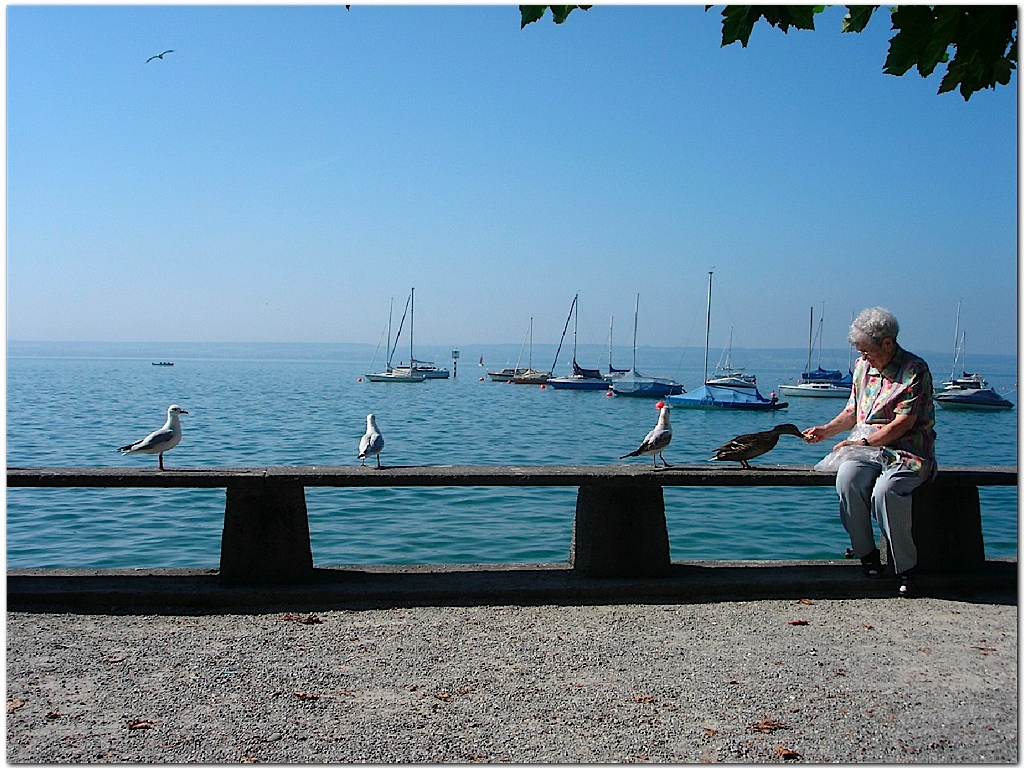
\includegraphics[width=300px]{images/DSC01957.JPG}\\
\textsc{Alimentando gaviotas y patos en el lago Constanza.} \end{center}

Avanc\'e 5~km y volv\'i a parar, mis piernas no quieren saber nada hoy. Da la
casualidad que era una playita, as\'i que --acord\'andome de que no me acuerdo
como es el Pac\'ifico-- me met\'i al lago, casi a la fuerza. Un poco sucio,
las piedras no dejan caminar (pero s\'i nadar), pero uno est\'a en Alemania
mirando a Austria en aguas de un gran lago sobrevolado tanto por aviones como
por dirigibles. \textquestiondown Vieron? De nuevo es la importancia de las
fronteras pol\'iticas: c\'omo uno siente diferente al acerc\'arseles. Es raro.

Pasando el mediod\'ia (\textexclamdown s\'olo 15~km en toda la ma\~nana!)
segu\'i viaje muy tranquilo, destino a Lindau si no pasaba nada. Y no pas\'o:
la ``Bodensee radweg'' est\'a muy bien marcada. Adem\'as est\'a llena de
turistas en bici, cosa que me encanta ver. Familias, parejas viejas y
j\'ovenes, amigos, todo el mundo viajando con las mochilas atr\'as y a pedal.
Ayer dorm\'i con un sueco que estaba haciendo un flor de viaje. Ahora
ven\'ia de Yugoslavia, Duvrovnik. Hoy segu\'ia por donde yo vengo, y se
babeaba en ``alemanglish'' con la ``Romantische Stra\ss e''.

Llegu\'e un poco temprano a esta maravilla de ciudad hist\'orica, las calles
son una preciosura; los edificios, una obra de arte. Ahora los miro desde el
faro al que acabo de subir, nunca v\'i uno tan lindo y adornado. Est\'a en la
punta de una escollera, que enfrenta a otra gobernada por un le\'on; recuerdan a
los lobos marinos marplatenses. D\'ia claro, un barco tur\'istico que cada media
hora entra y sale tocando sus bocinas, pocos turistas dandome vueltas alrededor
del faro, y dos regatas que salen del muelle. \textexclamdown Me encanta verlas!
Se mueven r'apido.

Com\'i banana ba\~nada en chocolate y una especie de caramelo pero que no es
caramelo. Delicia. \textexclamdown Qu\'e cambio de rumbo el m\'io, ehh! Por
fin los helados son un ``lujo'', ahora busco una buena relaci\'on
nutrici\'on/precio.

\textexclamdown Saludos alemanes hacia todo argentino que se les cruce!

Tute.

PD: Gustavo me espera (no sabe cu\'ando, como yo) con chivito al asador.
\textexclamdown Otra que el hijo pr\'odigo! \textexclamdown Ya lo veo a Felipe
quej\'andose! \textexclamdown Gracias, Gustav! Si va todo como lo planeo en
dos semanas llego a pedal a tu casa. Si me canso y tomo un tren, antes.
Adem\'as, tengo que pensar en el Sal\'on de Frankfurt. \textexclamdown Gracias
de nuevo!

\subsection*{Viernes 9 -- Immenstadt -- 60~km en 6:13 hs}

Aqu\'i se acaba de largar a llover, menos mal que ya estoy instalado.
\textexclamdown L\'astima que dej\'e toda el abrigo en donde me instal\'e!

Lindau estaba invadida de ara\~nas. \textexclamdown Llena de grandes telas
ocupadas por numerosas ara\~nas, en todos lados de la ciudad! Juro que ni pude
usar cabinas telef\'onicas, \textexclamdown incre\'ible! Nunca vi nada igual.

Hoy empec\'e con el bendito desayuno, acompa\~nado de una pareja alemana que
viajaba en bici por el lago. Lo sorprendente eran sus dos hijos, \textexclamdown
una de seis a\~nos! Charlamos un rato y me indicaron lo monta\~noso de mi ruta
para el d\'ia de la fecha. Como siempre, recib\'ia las noticias sonriente.

El clima amenazaba desde atr\'as, pero adelante el sol brillaba. La ruta, 508
creo, era con curvas seg\'un el mapa. Sub\'i a pedal unos 8~km (en vertical,
por poco necesito grampas y picos) por bosques. La cantidad de
curvas era imposible de dibujar en mi ahora poco detallado mapa. Desde arriba
ten\'ia una vista fenomenal, tom\'e muchas fotos. Cerros m\'as altos, mucho
bosque, casitas perdidas (buscaba caminos que las unieran pero nada, se
levantaban en medio del c\'esped), y abajo, el valle. Bajadas del 10\% seg\'un
carteles (que bajan 10 metros cada 100 recorridos) equival\'ian a 50~km/h sin
pedalear. Luego, suaves pero largas subidas; me desgastan m\'as que las de
mayor pendiente, porque intento hacer fuerza en lugar de entregarme a una baja
velocidad.

Par\'e en un banco de plaza mirando al valle. En algunos hosteles ofrecen
bidones de t\'e fr\'io, rojo y sin az\'ucar; tom\'e el que ten\'ia en la
botellita grande. Hab\'ia aviones por todo el cielo. Me sorprendi\'o el ver a
lo lejos mi misma ruta, que hac\'ia \emph{varios} minutos hab\'ia transitado.
Desde ahora har\'ia siempre eso: {\small V} cortas en c\'irculo, apuntando a
un mismo caser\'io (imaginen una pizza, lo cortado es el camino y el centro el
caser\'io). La sensaci\'on de no avanzar me cansaba, si bien el paisaje era
inmejorable. Menos mal pens\'e parar en Immenstadt porque estaba m\'as lejos
de lo pensado, aunque F\"ussen (destino inicial) estuviera a su vez m\'as
cerca de lo pensado: 60~km para el primero, 35 m\'as hasta F\"ussen. Imposibles
en el d\'ia de hoy.

Las altas y nerviosas monta\~nas suizas (antes lejanas) ahora serv\'ian de
fondo a las suaves, y ahora m\'as altas, sierras alemanas. \textexclamdown En
una bajada en recta llegu\'e a 74~km/h! En bici se siente m\'as la velocidad que
en cualquier veh\'iculo motorizado. Se la ve.

Luego de bordear un lago llegu\'e a Immenstadt a las 13:05. \textexclamdown Lo
not\'e porque de 13 a 14 cierran hasta los buzones en Alemania!
\textexclamdown No hab\'ia ni una \emph{B\"ackerei} abierta! Un super y una
fruter\'ia calmaron el hambr\'in. Esper\'e en una linda plaza central a que
abriera informaci\'on tur\'istica, y me indicaron una \emph{Gasthaus} donde
parar. \textexclamdown Cercana seg\'un los mapas, pero alta subiendo a la
monta\~na! Se nota la falta de aire en ese punto de la a\'un ciudad.
\textexclamdown Y se ve tan cerca!

Es la casa de una se\~nora de unos 70 a\~nos, m\'as simp\'atica que un perro
labrador; l\'astima que hablo poco alem\'an. Me di una ansiada ducha: en
subidas uno transpira densamente, y ni mis cejas de gallego pod\'ian
contenerla. Despu\'es sal\'i a recorrer la ciudad, momento en que empez\'o una
lluvia acompa\~nada de truenos. As\'i es que en una galer\'ia de una plaza
escribo mientras miro c\'omo la gente camina con paraguas (qu\'e envidia),
c\'omo se riegan las flores de los balcones, y escuchando las gotas (que
hac\'ia tempo no escuchaba, \textexclamdown espero no tener que hacerlo por
mucho tiempo!) sobre mi sombrilla.

Austria debe ser divino, en fotos desde Alemania con buena visibilidad se ven
sus picos nevados. Vi un cartel que indicaba una ciudad austriaca con marquita
``A'', a s\'olo 2~km. Lo segu\'i para pisar otro pa\'is pero un cartel de la
Uni'on Europea indic\'o, a la misma vez que cruzaba, que empezaba una autopista.
Volv\'i por mi camino con ganas de haber conocido.

Me espera ahora un panote de esos alemanes con semillas de cena, por s\'olo
\geneuronarrow{1}. \textexclamdown Parezco el vendedor de la panader\'ia!
Voy a ensanguchar una banana, y ma\~nana o pasado les contar\'e c\'omo estaba.

\subsection*{A partir del 10 de Septiembre -- El viaje desde Immenstadt}

\emph{Pas\'e varios d\'ias sin escribir mails, pero los le\'ia. Continuaba,
eso s\'i, escribiendo en mi maltrecho cuaderno. Antes de transcribirlo envi\'e
este resumen a un hermano, en que contaba c\'omo continu\'o el viaje, y c\'omo
regres\'e a G\"ottingen.}\\

\textexclamdown Hola Rami! Gracias por tu mail. Te escribo en breves l\'ineas
lo que sigue al diez: llegu\'e a F\"ussen y conoc\'i los grandes castillos, un
buen lago, monta\~nas altas, divinura. Hice la mitad del viaje tras un
ciclista alem\'an m\'as bueno que el pan lactal. Despu\'es segu\'i viaje por
la \emph{Romantische Stra\ss e}, \textexclamdown 100km! Cuando llegu\'e a
Landsberg y tuve problemas con hoteles llenos (s\'i, un poco por falta de
plata, pero fue m\'as bien una excusa) tom\'e un tren a Dachau
(\emph{Dajau}), ya que no sab\'ia como unirlo en bici del mejor modo, un
desv\'io de 50~km, ``\emph{not big deal}'' para el proyecto de circuito a
pedal.

Dorm\'i all\'a y conoc\'i el campo de concentraci\'on nazi, que luego de ver
libros lo \'unico nuevo fue la piel de gallina de estar pisando el mismo suelo
y respirando el mismo aire (al oler la madera de las literas me inquiet\'e
mucho, pero son reconstruidas) y pasando a trav\'es de la misma puerta
``\emph{arbeit macht frei}'' (``el trabajo los har\'a libres''), que para los
creyentes fue verdad: hijos de puta. Lo que s\'i me movi\'o diferente de lo
que ya conoc\'ia fueron los crematorios, ``\emph{dead chambers}'' (almac\'en
previo al crematorio) y c\'amaras de gas (me sorprend\'i en una sin saberlo y
el chorro de adrenalina fue suficiente como para necesitar acercarme a una
persona y sentirme un poco a salvo de la historia). Y me dej\'o pensando en
c\'omo un nazi, por m\'as fanatismo que tenga, puede creer que est\'a haciendo
bien, puede quererse creando tanto mal, y suponiendo que s\'olo fuera una
persona. Justamente tal vez por la cantidad y falta de personalidad uno puede
creer, como el nazismo pretend\'ia, que \'esas no son personas.

Un folleto de la historia de la ciudad, que empieza desde el 800dC, dice que
tristemente ahora el nombre Dachau no se asocia a la ciudad de artistas y
comercio en la ruta Augsburg-M\"unchen que era antes. Es verdad: lo dijo la
expresi\'on de la de informaci\'on tur\'istica al yo preguntarle; lo dice el
folleto; lo dijo un jud\'io sobreviviente (frase en la entrada del campo); lo
mostr\'e yo al preguntar por eso antes que por el castillo.

En el tren a Dachau pensaba ``qu\'e lindo que me lleve a G\"ottingen'' y as\'i
me di cuenta de que extra\~naba por lo que, luego de conocer all\'a:
\textexclamdown tren a casa! Y ac\'a escribo, desde mi {\small PC} y sin
Romantische Stra\ss e, y sorprendentemente para m\'i (a pesar de no haber
completado el viaje planeado) {\small CONTENTO}.

Me cans\'e de estar solo, es la raz\'on principal y verdadera. Traste y
piernas son un viol\'in, seguir\'e saliendo a correr seguramente. Me esperan
todav\'ia el sal\'on del autom\'ovil, el museo en Wolfsburg, y dem\'as cositas
``kinder'' que se ir\'an presentando.

Ese es el resumen, \textexclamdown ya mandar\'e el detalle! \textexclamdown No
se librar\'an de mi!

\textexclamdown Gracias por \emph{todos} sus mails! No saben qu\'e alegre los
leo y c\'omo me sirvieron durante el feliz pedaleo.

PD: La noche de ayer que estaba de fiesta por volver a casa despu\'es del
\emph{Viaje} tom\'e mi primer cerveza sin que me ofrezcan. Hace tres meses que
no tomo nada, y tomar vac\'io mientras esperaba el plato bast\'o para que mis
pasos (m\'as 100~km recorridos, y esta debe ser la verdadera raz\'on) ya no
sean tan precisos.

\subsection*{S\'abado 10 -- Immenstadt -- 0~km}

Hoy me levant\'e y llov\'ia, desde ayer sin parar. Encontr\'e poco por hacer,
casi que dependo de la bici. Claro, estar al pedo solo no es lo mismo que
acompa\~nado. Luego del suficiente desayuno sal\'i a caminar bajo la lluvia.
Recorr\'i, mand\'e cosas a casa por correo, compr\'e ``El amor en tiempos de
c\'olera'' (incre\'ible como escribe Gabriel Garc\'ia M\'arquez: hace una
prosa poetizada, con tantas palabras que m\'as de una vez necesito
diccionario), y tambi\'en un s\'andwich para almorzar.

Una ducha por el fr\'io; le\'i hasta que el ruido de la lluvia, tan
rom\'antico ayer a la tarde, me desesper\'o. Sal\'i de nuevo a caminar,
Immenstadt es una bonita ciudad. Me sent\'e en una galer\'ia de la plaza
central, y se ve\'ian los cerros al fondo siendo tragados por las nubes.
Camin\'e hasta la entrada del pueblo, se ve\'ia ahora la niebla
levant\'andose. \textexclamdown Se iban las nubes! Lo gris se mov\'ia, entraba
luz y dejaba de llover.

Pas\'e la \emph{Gasthaus} y sub\'i hasta la m\'inima capilla que se ve desde
mi ventana, divina vista tiene. Simpleza total. Donde ir\'ia el altar hay
im\'agenes que recrean a la crucifixi\'on. Cinco bancos de iglesia a cada
lado, y el v\'ia crucis externo, que parece una sucesi\'on de l\'apidas
rodeando la capilla. Un fresco en el alto techo era el \'ultimo detalle.
\textexclamdown Simple y hermosa!

Sub\'i a mi habitaci\'on y mir\'e por la ventana, vi al cielo ya no
homog\'eneamente gris, sino con las infinitas tonalidades de las numerosas
nubes tocadas por el sol, que se esconde.

Baj\'e a cenar luego de lecturas a las ``\emph{halb acht}'' (7:30 no 8:30,
menos mal que tengo apuntes). Ah\'i, siete amigos que promediaban los
cincuenta tomaban, com\'ian y re\'ian. Ninguno hablaba otro idioma adem\'as
del alem\'an, as\'i que les devolv\'i agradecido el ``\emph{Guten Apetit}''.
Por se\~nas (muy f\'aciles de imaginar) les pregunt\'e si eran ellos los que
anoche guitarreaban. Se escuchaba m\'usica t\'ipica alemana, pero cre\'i que
ven\'ia de la casa de al lado. S\'i, eran ellos, as\'i que me invit\'e a
unirme esa noche. ``\emph{Sehr Gut!}'', contestaron. Apenas empec\'e a cenar
me dejaron su Leberwurst, riqu\'isimo. Cuando termin\'e el pan fui a buscar
m\'as y notaron que no encontraba, as\'i que me dejaron el de ellos. No
contentos con eso me dejaron una salchicha ahumada, riqu\'isima. Tambi\'en me
ofrecieron Brandy (\'unica bebida alcoh\'olica aparte de la cantidad de vino y
cerveza) que a pesar de mi curiosidad por conocer negu\'e.

Sub\'i hasta que empezaran a guitarrear. Y vi el cielo libre de nubes, me
alegr\'o. Cuando baj\'e (con el diccionario alem\'an-espa\~nol) me ofrec\'ian
cerveza pero ya me daba verg\"uenza, as\'i que negu\'e hasta que insistieran.
Claro que no lo hicieron, \textexclamdown Murphy la ten\'ia clara al dictar
sus leyes! Estuvo buen\'isimo: una o dos horas de siete amigos alemanes
ebrios, cantando a coro y con dos guitarras su m\'usica tradicional. Me
preguntaron (con adem\'an de prestarme) si tocaba la guitarra. \textexclamdown
Me qued\'e con buenas ganas de cantarles ``El corralero'', \'unica que se y
por noches similares! Me animo a cantar por descarado, \textexclamdown pero de
la guitarra m\'as vale mantenerme alejado! Me contaban que esa tarde caminaron
hasta la cima de no-se-qu\'e-cerro, que no era gran cosa sino era por la
lluvia, el barro y la niebla. Son gente de un pueblo a 100~km de Karlsruhe,
turistas por el fin de semana, y cantan por hobby. La que m\'as me gust\'o
fue ``\emph{Kapitano}''. Me sorprendi\'o su inter\'es en que nos
entendi\'eramos. \textexclamdown Igual creo que me perd\'i diecisiete chistes!

\textexclamdown Como a las 10 pm nos dio sue\~no! La guitarreada empez\'o a
las 8 pm, gran diferencia en las costumbres con nuestras pampas. Nos acostamos
luego de mirar el claro cielo con poco de niebla. Cama c\'omoda como pocas
veces, la disfrutar\'ia hasta las 8 am, hora en que nos despertar\'ian.
\textexclamdown A disfrutar de la ma\~nana en Alemania! Y c\'omo lo har\'ia
esta.

\subsection*{Domingo 11 -- F\"ussen -- 50~km en 2:15 hs}

Hoy me levant\'e a las 8 am, no se ve\'ia un chosno. La niebla ni siquiera
dejaba ver el color del cielo, y estaba un poco fresco. Sal\'i igual a pedalear
luego del desayuno: los pron\'osticos indicaban lluvia para la tarde y no le
erran. Suelo h\'umedo pero no mojado; en la noche no hubo chaparrones.

Apenas sal\'i de los l\'imites de Immenstadt\ldots\ \textexclamdown
desapareci\'o la bruma! Mir\'e atr\'as y la ciudad estaba inundaba por densas
nubes, muy sorprendente. Ve\'ia niebla arriba en los cerros o en mi ex-ciudad,
pero no en mi camino, cosa que me alegr\'o por poder ver los siempre enormes
paisajes. Los caracoles de subida que anunciaban mi mapa no fueron tan
interesantes (o me equivoqu\'e de ruta), pero todo el camino presum\'ia de
belleza en cada kil\'ometro.

Me pas\'o un ciclista rutero, y creo que me pregunt\'o si iba a F\"ussen. Le
dije que s\'i: si preguntaba si ese era el camino la respuesta era igual. Nos
cruzamos otra vez, otra y despu\'es otra. En las bajadas yo pedaleaba as\'i
que me acercaba, \textexclamdown pero \'el sub\'ia como si viajara en bici!
Entonces desaparec\'ia. En la tercera vez que lo encontr\'e, parado
sac\'andose abrigos de las piernas, fren\'e y empezamos a charlar. No se
porqu\'e me dijo que casi no hablaba ingl\'es: vivi\'o un a\~no en Orlando
Florida trabajando para ``\emph{Universal Studios}'', donde ve\'ia a diario la
r\'eplica del gran castillo que estaba yo por visitar: \emph{Newschwanstein}.
De Essen el hombre, se sorprendi\'o de que la mochila fuera todo mi equipaje.
Yo me enorgullec\'i de eso, y le cont\'e mi viaje. Nos sacamos foto en un lago
(parezco el turista japon\'es) y seguimos viaje. Me llev\'o como lech\'on pal'
pueblo, pero como cortaba el viento se sinti\'o poco. As\'i que llegu\'e al
mediod\'ia y con traste nuevo, despu\'es del descanso de ayer y pocas horas de
hoy. Al entrar al pueblo lo desped\'i pero lo cruc\'e dos veces m\'as: al
salir de las oficinas (\'el entraba), y al subir a los castillos m\'as tarde
(\'el bajaba).

Qu\'e diferencia: \textexclamdown hoy no me alcanz\'o el tiempo! Dej\'e bolsos
y sal\'i en la bici al centro tur\'istico. Calles estrechas y zigzagueantes,
casitas antiguas con carteles de metal sobresaliendo, galer\'ias con no
demasiada gente\ldots\ en una cuadra hab\'ia varias casitas muy similares,
pero de colores tan distintos que parec\'ia un dibujo de primaria. Almorc\'e
una bomba de panader\'ia inc\'omoda (ten\'ia forma de bomba, literalmente)
sentado en una fuente, y mirando y escuchando a un trompetista. Al encarar
hacia los castillos escuch\'e una gran banda. Me acerqu\'e y era estilo
militar, con muchos instrumentos de viento y director al frente. Las bandas
numerosas me emocionan, la observ\'e hasta que me picaron las hormigas (que no
despert\'e a prop\'osito).

Me separaban 5~km hasta los castillos. Me sorprendi\'o la ciclov\'ia, por su
cartel de ``\emph{Romantische Stra\ss e}'', ruta que seguir\'ia con \'unico desv\'io
hacia Dachau. \textexclamdown Los folletos muestran 20 pueblos con detalles
interesantes por conocer en esas decenas de kil\'ometros de calle rom\'antica!

Cuando divis\'e el castillo grande y m\'as nuevo sent\'i lo mismo que al
encontrar el lago Constanza: un punto de referencia grande en los planes del
viaje. Emocionad\'isimo sub\'i hasta encontrar el ``\emph{Ticket center}''. No
se r\'ian del viajero, pero juro que se parec\'ia a un aeropuerto. Lleno de
gente, una cola larga hasta las 4 ventanillas de venta, y monitores indicando
las ``pr\'oximas salidas''. ``Salgo a la hora que quiero'' pensaba yo, hasta
que el vendedor me pregunt\'o:

\subparagraph{}\label{ssub:hayGuia} --- \textquestiondown Gu\'ia en
ingl\'es?\\ --- No, gracias. Voy por mi cuenta.\\ \hangindent=1cm

Pero resulta que no est\'a permitido, as\'i que me citaron a las 13:15 en
\emph{Hogenschwangau} --menos mal que fue el primero-- y a las 15:25 en
\emph{Newschwanstein} --menos mal que fue el segundo.

Lo primero que encontr\'e camino al primero fue un hermos\'isimo lago rodeado
de monta\~nas bajas y boscosas. Las monta\~nas m\'as altas todav\'ia tienen
nubes atascadas, \textexclamdown que no se pinchen y se largue a llover!

Encontr\'e todo incre\'iblemente lujoso (como es de esperarse en un castillo,
creo), adem\'as de lindo. Lleno de condecoraciones, le pregunt\'e al gu\'ia si
la familia real iba a la guerra. ``Algunos mostraban su valent\'ia'', fue toda
su explicaci\'on. Dise\~no a la antigua, con almenas (esos ladrillos cuadrados
en los que uno imagina escondido detr\'as a un arquero); y color a la
vanguardia: anaranjado y amarillo. Vista que asombra. Tras una ventana hab\'ia
algo similar a un telescopio, pero en vez de apuntando al cielo, apuntaba a lo
que eran entonces las construcciones del nuevo castillo de Ludwig II:
\emph{Newschwanstein}. Luchito para los amigos --o luch\'in, porque me qued\'e
con dudas sobre su preferencia sexual seg\'un charlas de la gu\'ia-- segu\'ia
las construcciones de su nueva casa desde su casita anterior. \textexclamdown
Locura Real! Para visitar al ``vecino'' se baja una monta\~na y se sube a la
otra.

Baj\'e a ``\emph{ticket center}'' para subir al otro castillo por donde lo
hacen los colectivos, que es m\'as largo y en curvas que el camino peatonal.
Es una ``{\small V}'' corta que sube a la monta\~na, de sentido \'unico y no
mucho lugar para maniobrar, con sem\'aforos en la salida y la llegada.
Esper\'e bastante al verde del sem\'aforo abajo, hasta que me pas\'o un
colectivo (usan controles remotos para cambiar las luces) y pedale\'e
tranquilamente pero sin parar, viendo cada vez m\'as el lago Alpsee. Al llegar
a la curva empezaba a caer una fina lluvia, que el bosque mantuvo en sus hojas
hasta que llegu\'e al techo de la parada de colectivos, cercana al
``\emph{Marienbr\"ucke}''. ``\textexclamdown Pararse en ese puente justifica
un viaje a Europa, Tu!'', ya hab\'ia advertido mi t\'io. Dej\'e la bici
ah\'i y sub\'i al puente para corroborarlo.

Se siente hermoso tan solo describirlo. Lo construy\'o primero un
rey para disfrutar de la vista al valle. Abajo corre un curso de agua, y
justito abajo en vertical hay una olla donde desemboca una
cascadita, que si no fuera por los 34 metros de altura dan ganas de tirarse.
Luego Ludwig embelleci\'o el puente para ver, aparte del paisajazo y lagos
\emph{ForggenSee} y \emph{BunnwaldSee}, a su nuevo ejemplo de excelent\'isima
arquitectura, el castillo que ahora visitar\'ia. El mal clima permiti\'o una
particular vista. Sin taparme las monta\~nas y lagos (los hac\'ia parecer
m\'as lejanos), las nubes se apoyaban sobre los picos m\'as altos.
Bell\'isimo. \textexclamdown Con sol se debe ver hasta el Mar del Norte!

Luego esper\'e 20 minutos en la entrada del castillo bajo la lluvia, rodeado
por los blancos muros, las monta\~nas y la ca\'ida de agua. Ya en la visita,
me impresion\'e con las dos millones de partes que componen el brillante
mosaico del suelo de una sala, con la apertura al p\'ublico por parte del
estado s\'olo seis semanas luego de la muerte del sin herederos Ludwig II, y
con su habitaci\'on que merece p\'arrafo aparte. Y todo esto, sin contar que
no lograron terminar la obra antes de su muerte, y de hecho actualmente hay
habitaciones vac\'ias.

Su habitaci\'on da a la cascada, as\'i que siempre hay ruido a la fuente de
vida (el libro de la n\'omada del desierto africano me conmovi\'o, como
notar\'an). Hubiese descripto el estilo como similar a la catedral de
Estrasburgo pero gracias a que me enchufaron gu\'ia ahora s\'e que es
``g\'otico''. La cama parece en s\'i misma una catedral, con el techo inundado
de ornamentos en madera. No me salen las palabras para describirlo, y cuando
estudi\'e G\'otico seguro las memoric\'e. Las paredes y columnas (todo de madera
oscura) tienen un trabajo de precisi\'on incre\'ible: \textexclamdown 4 a\~nos
de trabajo llev'o esta sala! La puerta se camufla entre los adornos del estilo y
me encant\'o la gran cerradura y picaporte. Su sill\'on de lectura lo tall\'o un
duende, no un humano porque sus manos ser\'ian demasiado grandes y menos
precisas. Me sorprendi\'o su capilla propia, de 2$\times$2 m, con lugar para el
Sant\'isimo y todo. Los reyes ten'ian l'inea directa parece.

En las pinturas de guerra (cientos de guerreros a pie o caballo clav\'andose
lanzazos) no se ve sangre por ser considerada ``anti-est\'etica''.
\textquestiondown Y desde qu\'e aspecto la guerra lo es? S\'olo, al menos y
mir\'andola con demasiado cari\~no, el esp\'iritu de entrega absoluta por una
causa que algunos creen justa. Pero es eso justamente lo que evitaron mostrar
en las grandes pinturas del enorme comedor. Sobre tama\~no de cocinas, \'esta
aproximadamente ocupa una hect\'area. Hab\'ia una mucho m\'as chica para la
servidumbre seguro, aunque me sorprendi\'o no usaran la misma.

En los mapas de la zona no se ven cercanos los lagos al castillo, por eso no
entend\'ia las postales con todo juntito. Es que los castillos est\'an altos
en la monta\~na; desde all\'i se ve el lago perfectamente, y la ruta
rom\'antica saliendo hacia el Norte. Aunque en realidad no est\'an en la punta
de un cerro, como en las suaves colinas del centro de Alemania: el precipicio y
las rocas de aqu\'i imposibilitar\'ian la construcci\'on.

A la salida camin\'e hasta mi bici y me abrigu\'e para evitar mojar mi ropa en
la bajada, hab\'ia dejado de llover. Guard\'e el cuaderno en una bolsa junto
con un vaso alem\'an nuevo (\textexclamdown por fin uno que me encanta!), y
at'e el candado atr\'as porque se caer\'ia si lo dejaba sujeto al cuadro.
Luego de pedirle a un chofer que me diera luz verde, me tir\'e. Mientras,
quienes esperaban al siguiente colectivo me miraban, \textexclamdown no se si
envidiosos, o como a un loco!

No anduve muy r\'apido, era peligroso en bajada y con agua, entre el humilde
ancho del camino y el precipicio. Hasta donde los nervios me permit\'ian.
Usaba los dos frenos pero, acostumbrado al peso de las mochilas, us\'e
demasiado el trasero y en una curva di una derrapada, que no por exagerada
como por la velocidad y condiciones del camino, es que me dio El Susto.
Siempre me siento controlado en dos ruedas, pero sobre agua nunca: me di
varios y sorpresivos golpes por no medir bien los l\'imites. Siempre recuerdo
con cari\~no uno yendo a la escuela, porque era invierno y estaba todo abrigado,
as\'i que s\'olo se escuch\'o la campera, la mochila y los pedales raspando
contra la calle. Cuando no pasa nada malo es divertido pero ac\'a no pod\'ia
asegurar la misma suerte. Por suerte (seamos sinceros, \textexclamdown por
perfecto dominio!) la cola de la bici volvi\'o a su lugar y continu\'e la
bajada, hasta el primer techo que encontr\'e en el punto comercial.

Foto a la cara de felicidad despu\'es de la adrenalina, \textexclamdown y a la
caliente ducha del hostel, sin paradas! Si ma\~nana llueve, envuelvo el equipaje
en bolsas y sigo vestido como hoy, seco y calentito.

Volv\'i por una gran plaza y de nuevo las encontr\'e sorprendido: bolsitas de
basura en un dispenser para recoger los restos de los cachorrines, y mantener
as\'i el pasto y caminos limpitos. Otro comentario: vi varias veces caballos
de equitaci\'on y ni\~nos entrenando, no saben lo bellos que son. A los
caballos no les cortan los crines ni la cola, son de color chocolate,
musculosos y de todos los tama\~nos. El ni\~no, o ni\~na m\'as generalmente,
con botas largas de cuero, pantal\'on blanco o negro, camisita blanca y
casquito negro, sentados derechos sobre el animal que camina con buena
presencia. Me encantan. Tambi\'en cruc\'e dos personas en bici con demasiados
bolsos y entonces me fij\'e en su banderita: ``la vuelta al mundo''.
\textexclamdown Que l\'astima \'ibamos en sentido contrario y no pude charlar!
El sue\~no del pibe.

Llegado a la ducha, mi cara cambi\'o\ldots\ \textexclamdown y no para bien! Esta
ducha es como otra que ya tuve: una incre\'ible presi\'on, y el agua tan
pulverizada que de verdad arde. Panza y cabezas, resguarecidas.
\textquestiondown Pueden creer que una ducha haga mal? \textexclamdown Es como
comer un poco de pan de salvado y caiga pesado! Y uno entra con esperanzas de
salir renovado, relajado, descansado; y sale todo maltrecho como si viniera de
un viaje en bici bajo lluvia. \textexclamdown Incre\'ible! Y ya lo mencion\'e,
\textexclamdown las nuevas experiencias que tengo en Alemania son dif'iciles de
olvidar!

\subsection*{Lunes 12 -- Dachau con trampita -- 100~km en 5:32 hs.}

Hoy fue un buen d\'ia largo. Empez\'o temprano con un desayuno en una luminosa
galer\'ia, con buena vista a un parque. Despu\'es de pasear un poco por las
cercan\'ias de F\"ussen hasta por fin encontrar la Romantische Stra\ss e para
bicis, la segu\'i. Es comod\'isima, bien se\~nalizada y lejos de los autos.
Paisajes incre\'ibles, una niebla levant\'andose, y el gran castillo de fondo
por largo tiempo acompa\~nando, rodeado de cerros y de bosques. Clima bastante
fresco y cielo de todos los colores: pod\'ia salir el sol como venir un
tornado. Se decidi\'o por lo que los pron\'osticos predec\'ian: nublado sin
siquiera llovizna.

Conoc\'i \emph{Wieskirche}, una iglesia con m\'as fama que Chatr\'an.
Entr\'e pensando ``porqu\'e tanto espamento'' y entonces entend\'i. En vez de
ser con forma de cruz y techo de la misma altura, en el medio se levanta una
b\'oveda como joroba, que del lado interno presenta frescos; todo bello,
lujoso, y viejo pero preservado perfectamente. Saqu\'e la foto a una firma
grabada en uno de los ornamentales bancos de madera del a\~no 1800, mi t\'io
informa que las hay mucho m\'as viejas. Me impresionan siempre los \'organos y
el lugarcito desde donde el sacerdote dar\'ia la homil\'ia, un piso m\'as
arriba sobre un costado de la nave central. Siempre con incontables adornos.

No me cans\'e de sacarle fotos al paisaje y tambi\'en al cielo, siempre
cambiante. Este cielo les har\'ia creer que soy buen fot\'ografo y todo.
\textquestiondown Vieron los cielos que uno ve pintado en acuarelas, o que se ve
en un campo e inspira ganas de pintarlo? Bueno, ac\'a est\'a todos los d\'ias,
uno lo puede ver mal por falta de sol o bello por los infinitos colores que lo
decoran. Las formas de las nubes, las avionetas apareciendo y
desapareciendo\ldots\ \textexclamdown Interesante mientras no llueve!

Al salir de \emph{Wieskirche} hay una capillita de las que a mi me gustan, de
5m$^2$, con figuras de la crucifixi\'on y un fresco de Jes\'us atado durante
los azotes, todo ensangrentado, que no dej\'o de impresionarme. Encorvado y
sufriente. Para colgar cerca de los cuadros de guerra de \emph{Newschwanstein}
estaba. Cre\'i que esas im\'agenes s\'olo se ve\'ian en la pel\'icula ``La
Pasi\'on'' pero vean, en esta capilla que ni siquiera a ello llega, hay un
cuadro vaya uno a saber de qu\'e a\~no. Hace pensar, por la crudeza, en lo que
uno piensa luego de ver esa pel\'icula.

Esta ciclov\'ia rom\'antica pasa por lo lindo de las ciudades lindas, con lo
cual los 100~km no se permitieron un segundo de aburrimiento o gran cansancio.
En un pueblucho cualquiera, en una fuente cualquiera de una plaza cualquiera,
hay una estatua de bronce de un gordito pelado, sonriente, con los pies bajo
el agua y la mano tocando la superficie, como probando la temperatura. Sus
chancletas esperan al lado de la fuente. \textexclamdown Todo est\'a adornado!
Vi lo que la vieja me describ\'ia antes de mi viaje, pero cerca de G\"ottingen
en realidad: las dobles ventanas con adornos en el medio, cortinas desde la
mitad para abajo, detalles que hacen de una casa un hogar pero que no las ve
s\'olo la familia sino cada transe\'unte. Entr\'e en una iglesia de otro de
estos pueblos y justo ensayaban con el \'organo. Otro aderezo m\'as, esta vez
para oir.

Luego, y cuando promet\'i no parar m\'as para poder llegar a Landsberg, par\'e
para ver a un avi\'on que sub\'ia y bajaba, y sub\'ia y bajaba, todo el
tiempo, y cambiaba de altura bastante r\'apido. Tiraba paracaidistas
descubr\'i luego, siempre de a tres que se dejaban en ca\'ida libre por un
rato y luego los abr\'ian. El avi\'on se perd\'ia constantemente entre las nubes
bajas, a los aventureros les debe haber hecho m\'as picante la experiencia.
Entonces promet\'i no parar m\'as, y a la vuelta de la curva hab\'ia, armada con
le\~nos que por ac\'a abundan, la forma de la fachada de una casa. En vez de
mantenerlos embolsados para guardarlos les dieron una forma m\'as particular y,
claro, bella. Par\'e para sacar foto mientras la molestia de no cumplir con el
plan se mezclaba con la alegr\'ia de no poder dejar de sorprenderme.

Luego segu\'i los 30~km hasta Landsberg, pensando en c\'omo unir Dachau, y
cuantas noches usar en ``desviarme'' hacia el Este de lo conocido (al menos por
mis folletos). Me interrumpi\'o los pensamientos un avi\'on grande, parec\'ia
los que usan los bomberos para los fuegos en bosques pero de colores militares.
Enorme y a muy baja altura, segu\'ia el curso del r\'io que yo bordeaba.

Llegu\'e a la ciudad y me fascin\'e con su centro tur\'istico. En
informaci\'on me indicaron que todo estaba lleno, me mandaron a la estaci\'on
de trenes que quedaba cerca, pero ah\'i me dijeron que no hay habitaciones. Un
hombre vio que necesitaba ayuda, y muy amablemente me acompa\~n\'o media
cuadra hasta una pensi\'on que ofrec\'ia n\'umeros telef\'onicos a falta de
recepcionista. Al mostrarle mi falta de tel\'efono fue a buscar el de su casa,
pero no atend\'ian. Lo vi tan hospitalario que le ped\'i indirectamente un
suelo para echar mi bolsa de dormir, pero me contest\'o evasivamente, aunque
de buen modo, que no sab\'ia quien pod\'ia prestarme un suelo.

S\'olo quedaba un hotel a \geneuronarrow{55}, la temporada alta se hace
sentir. A rega\~nadientes acept\'e, pero cuando sub\'i y vi que la
habitaci\'on era fea y oscura, hice unos llamados para solucionar unas cositas
todav\'ia de la tarjeta y ped\'i el checkout. \geneuronarrow{30} de llamadas
(\textexclamdown terrible!) y verificaron que no me haya ba\~nado. Todo estaba
bien: limpi\'e el inodoro que ven\'ia necesitando desde hac\'ia kil'ometros. No
me importaba si ten\'ia que no dormir, o dormir sentado en el centro
tur\'istico, pero no dejar\'ia la plata de dos o hasta tres noches en un lugar
que no me gustara. Mientras empacaba la bici pens\'e en tomarme un tren a
Dachau: solucionaba el ``problema'' de c\'omo unirlo, dormir\'ia bien
(r\'apida y astutamente descart\'e la opci\'on de prescindir de cama) y al
otro d\'ia seguir\'ia la ruta planeada.

Y as\'i fue, para completar los 50~km que restaban a Dachau tuve que tomar
tres trenes (me estoy poniendo canchero con el manejo en tren por Alemania)
pero fue barato y no muy inc\'omodo. El problema es que al subir corriendo al
pr\'oximo tren empezaba a pensar: ``\textquestiondown no me habr\'e olvidado
algo en el anterior?'' \textexclamdown Ninguna respuesta servir\'ia en este
nuevo tren! De todos modos y por suerte siempre eran respuestas negativas.

En el tren pensaba: ``qu\'e hermoso que este tren me lleve a G\"ottingen''. Y
entend\'i entonces que estaba extra\~nando, y tal vez por eso quer\'ia hacer
100~km y no parar en ciudades lindas como Landsberg, tal vez por eso estaba
gru\~n\'on. Tambi\'en me ten\'ia inc\'omodo que ya me quedaba de nuevo sin
plata, pero esa era la excusa. Decid\'i conocer Dachau y al d\'ia siguiente
tomarme un tren a casa; los 15 minutos de viaje que todav\'ia faltaban fueron
euf\'oricos. \textexclamdown Qu\'e alegr\'ia! \textquestiondown Porqu\'e, si
no hago lo que quer\'ia? Porque hice {\sl mucho m\'as} de lo que quer\'ia, y
ma\~nana voy a volver a estar c\'omodo y sin extra\~nar. Como en casa,
despu\'es agradec\'i a Gustavo que pudiera sentir esto en Alemania. As\'i,
cada vez m\'as contento, llegu\'e a Dachau.

Baj\'e del tren y segu\'i al mal\'on, que se iba r\'apido como si vivieran en
Buenos Aires. Era para el otro lado del centro y me di cuenta por la falta de
luces, sin embargo me sorprendi\'o, pues supuse que la mayor\'ia encarar\'ia
para all\'a, donde necesito. Le pregunt\'e a un chico que jugaba al basket y me
mand\'o al lejano hostal, que no fue dif\'icil de encontrar.

\textexclamdown Hostal canchero y moderno como pocos! Y con el precio de
hostal juvenil. L\'astima que no ten\'ian lugar. Puta suerte, ya eran las 21 y
estaba estrenando las luces de la bici, quer\'ia llegar a alg\'un lugar e
instalarme. El recepcionista, un no-joven muy servicial, me indic\'o una
\emph{Gasthaus}.

\subparagraph{}\label{ssub:hostalLleno} --- Un minuto, llamemos antes para ver
si tambi\'en est\'a llena -- contest\'e.\\ --- Bueno, \textexclamdown ah\'i
ten\'es un p\'ublico!\\ \hangindent=1cm

No esperaba esa respuesta, pero ten\'ia la tarjeta telef\'onica con que
llamaba a Gustavo. La nueva casa ten\'ia lugar, y lo reserv\'e con gusto.

Tambi\'en fue f\'acil llegar, todo por avenidas, siempre tomando la
bifurcaci\'on izquierda. Estaba al lado de Informaci\'on Tur\'istica y del
castillo, pleno centro y barat\'isimo por ser \emph{Gasthaus}. Cuando me
dieron las llaves de la habitaci\'on n\'umero 1 sent\'i endorfinas por todo el
cuerpo, \textexclamdown por fin! M\'as de 12 horas de viaje de puerta a
puerta. Guard\'e la bici lo m\'as relajado que pude, y al entrar pensaba que
por el doble de ese precio estar\'ia durmiendo ahora en un lugar feo y
planeando c\'omo llegar a Dachau, al otro d\'ia, en bici. Imposible de
pedalearlo, adem\'as, luego de los 100~km de hoy. Fue una buena decisi\'on.

As\'i que me relaj\'e, com\'i una gran ensalada con pollo (\textexclamdown
tuve que gastar de todos modos aquel no malgastado dinero!) y tom\'e la primer
cerveza de mi vida sin que me ofrezcan. Mitad mientras esperaba el plato,
mitad durante la sabros\'isima cena, as\'i que, y luego de pedalear 5 horas
(la verdadera raz\'on), ya los pasos no ser\'ian tan precisos. El lugar era
precioso, todo de madera, con doble ventana a falta de doble vidrio, vasos
alemanes sobre las alacenas, pinturas con im\'agenes t\'ipicas del lugar, diez
grifos rodeando la barra para cada tipo de cerveza\ldots\ un sue\~no t\'ipico.
Lo bueno es que mientras cenaba sonre\'ia solo, estaba empezando a asimilar y
pensar en todo lo que hice, en vez de planear qu\'e me esperar\'ia ma\~nana,
por primera vez en semanas. Ya estaba, \textexclamdown gracias por
acompa\~narme, piernas! Y todos esos pensamientos est\'upidos luego de cumplir
euf\'orico con algo propuesto. Mor\'ia por contarle a alguien pero no ten\'ia
el tel\'efono habilitado en mi habitaci\'on, menos mal porque me terminaba de
secar, sino. Y salir de mi hogar por fin encontrado por un tel\'efono, ni
ebrio.

Quise pagar con monedas pero no llegaba, as\'i que pagu\'e con el \'ultimo
gran billete. Los guachos notaron mis intenciones y el vuelto fue todo en
monedas, la mochila pes\'o un 20\% m\'as desde esa cena. Ba\~no de inmersi\'on
(con ese ocioso chorro, media hora esperando a que se llene la tina) y me puse
la tercer muda de ropa que no hab\'ia usado en todo el viaje, y su \'unico
olor era el del chocolate derramado cerca de Hann M\"unden, el primer d\'ia de
viaje. Vida nueva, una gran alegr\'ia. La mochila tuvo nuevo lugar
porque us\'e tambi\'en el jean poco engrasado y el buzo polar amarillo por el
fr\'io, que ocupa m\'as lugar que una almohada.

As\'i que dorm\'i perfectamente en una c\'omoda cama. Y ma\~nana al castillo,
info tur\'istica, y el campo de concentraci\'on de la II~Guerra Mundial para
terminar en la estaci\'on de tren. Todav\'ia no me imagino c\'omo ser\'a pero
de todos modos pienso poco, ya lo ver\'e.

\textexclamdown Qu\'e Lunes tuve! Otra que rutinario. Siempre me gusta pensar:
``hoy me levant\'e en F\"ussen'', y no puedo creer que todo haya sido en un
solito d\'ia. Pensar que el tiempo siempre se nos escapa como arena de las
manos, estando de viaje cambia todo. Ni les cuento en bici, que ver un ganso
es una actividad interesante. En la entrada de Wieskirche vi dos  cruzando la
calle, tuve que frenar como en los dibujitos. No aceleraron el paso, iban
graznando al cultivo de al lado para picotear el suelo. Uno atr\'as del otro y
moviendo la colita para caminar, como las palomas mueven la cabeza. Hasta eso
es interesante.

\textexclamdown Eso es \emph{todo} para este Lunes!

\subsection*{Martes 13 -- Dachau}

(\textexclamdown Menos mal que escribo porque cont\'andole a Gustavo me doy
cuenta que ya me olvido de cosas, importantes como nombres! O c\'omo era $x$
lugar donde dorm\'i.)\\

Desayun\'e abajo, en otra sala igualmente decorada en alem\'an. Me encantan
los cereales alemanes. Fui a informaci\'on tur\'istica y abri\'o en los diez
minutos que me llev\'o ver los folletos de la entrada, ninguno interesante
para m\'i. Mucho sobre arte. Entr\'e, y para ser discreto pregunt\'e qu\'e
cosas interesantes hay para conocer en Dachau. Me cont\'o mucho del arte,
galer\'ias de fotos, folletos con historia, el castillo que hab\'ia a una
cuadra de distancia. Le pregunt\'e sobre el campo de concentraci\'on y lo
indic\'o en un mapa, con una expresi\'on no tan sonriente que tal vez fue
s\'olo mi sensaci\'on. ``Por ah\'i los llaman diferente, ac\'a'' pens\'e al
ver los folletos en alem\'an, pero no creo porque en ingl\'es tambi\'en
dec\'ian eso: ``\emph{concentration camps}''.

Fui primero al castillo y el gris homog\'eneo cielo empez\'o a regalar
no-bienvenidas gotas de agua. Los parques del castillo hermos\'isimos,
mientras que el castillo no es tan imponente. Desde all\'i arriba se ve\'ian
edificios de M\"unchen, que no s\'e porqu\'e no muero por conocer. 18~km
solamente. Escapo a las grandes ciudades viajando en bici parece.

Apurado por la lluvia, busqu\'e mi bici y llegu\'e hasta el lejano campo sin
mojarme demasiado, los \'arboles cubren. En la entrada recibe la frase de un
sobreviviente: ``Dachau ya no es m\'as el nombre de una ciudad, ahora es el
triste nombre de todos los campos construidos en esta zona'', o algo as\'i
daba a entender. ``Pobres pobladores'' pens\'e, y pens\'e en la mujer de
informaci\'on tur\'istica. El folleto que ella me dej\'o de historia indica
eso: antes del 1.933 Dachau era la ciudad de artistas y comercial en la ruta
Augsburg-M\"unchen. Ahora es el recuerdo de la triste y cercana historia del
gran pa\'is que ahora es. Barat\'isimo entrar, hab\'ia dos grupos recorriendo,
uno de turistas y uno escolar, los dos en alem\'an.

Mucha informaci\'on, varias fotos, no demasiada dura crudeza (s\'olo la
realidad, y opacada porque est\'a reconstruido y no como realmente fue).
Siempre me imagino a esa \'epoca en blanco y negro, se que porque las
im\'agenes lo son pero lo imagino as\'i de todos modos: los largos tapados de
los que llegaban, los grises y gastados uniformes ``cebra'' que les
impusieron, los uniformes nazis, el clima gris y lluvioso que justo me
toc\'o\ldots\ las paredes sin pintura, las literas de madera. Por eso me
cuesta entender que el verd\'isimo pasto que estoy viendo tambi\'en exist\'ia.
O la blanqu\'isima nieve. Es incre\'ible. Le\'i mucha informaci\'on que es
parte de la historia, para el que ley\'o del tema nada nuevo bajo el sol.
C\'omo lleg\'o esa tiran\'ia al poder, c\'omo lleg\'o ese poder a ese imperio,
c\'omo ese imperio logr\'o una discriminaci\'on tan bruta y casi legitimada
por la poblaci\'on, al menos ignorada. S\'olo cambia el estar ah\'i, no lo
est\'as leyendo en casa, en un puf argentino, sino ah\'i donde 50 a\~nos antes
se paraban en atenci\'on durante 3 horas por no haber hecho prolijamente las
camas\protect\footnote{En su libro ``El hombre en busca de sentido'', el
psiquiatra sobreviviente Viktor Frankl relata que luego de su viaje de casi
tres d\'ias desde Auschwitz hasta aqu\'i, parado en un tren hacinado, debi\'o
pasar la noche junto a sus compa\~neros cumpliendo esta condena. Pas\'o
``gozoso'' esas horas de fr\'io, pues el nuevo campo no ten\'ia ``hornos'' ni
``chimeneas''. Frankl relata de modo concreto los sentimientos de los reclusos
y guardias en su ``vida cotidiana'', centr\'andose en las razones por las que
algunos se dejaban morir, mientras que otros continuaban pensando en su
futuro.}. \textexclamdown Donde estaban encerrados por ser! Ah\'i mismo.

Del museo informativo camin\'e a las barracas, solo dos hay. Las literas de
tres pisos, los ba\~nos, del otro lado las nuevas literas de cuando empezaron
a traer no s\'olo presos pol\'iticos sino, directa y simplemente, jud\'ios y
otros ``indeseables''. Son tambi\'en de tres pisos pero sin divisiones
laterales, as\'i era m\'as f\'acil llevar la superpoblaci\'on. Antes del viaje
hab\'ia visto una pel\'icula sobre un periodista que hizo una ferviente
propaganda anti-nazi, hasta que le llevaron sus anteojos sucios a la esposa
como documento no oficial de su muerte. Lo enviaron ac\'a, Dachau; fue el
primer campo y al principio era para ellos, todav\'ia no era con fines
raciales de exterminio.

Luego, caminata por la calle central, al medio de lo que alguna vez fueron las
30 barracas (en su per\'imetro hay ahora piedras) hasta los nuevos monumentos
y crematorios. Ah\'i s\'i se sinti\'o diferente. Bueno, qu'e se yo\ldots\
descripciones hay en cualquier libro sobre la \'epoca, pero a mi me hizo
pensar en c\'omo un soldado nazi --y por m\'as ideales que tenga-- pueda
querer hacerlo, o quererse haci\'endolo. Si ellos creen que no eran humanos
bueno, supongamos que nosotros lo hacemos con nuestras vacas o perros, que ya
me parece una falta de respeto por el sufrimiento de las personas. Inclusive
as\'i es imposible. Tan terrible, t\'etrico, oscuro, oloroso, sucio. Nido de
enfermedades. No existe raz\'on ni pasi\'on, no se entiende. Ser\'a la
inocencia que espero nunca perder la que me deja sin palabras.
\textquestiondown Saben la adrenalina que da el solamente caminar por esos
lugares? Estaba tan as\'i que hasta me molestaba que sacaran fotos, que
hablaran, cosa totalmente natural en un museo a la memoria, un museo de
Historia para concretar ese ``nunca m\'as''.

Conocido esto que me despertaba tanta curiosidad y ahora despert\'o nuevas
cuestiones y afirmaciones, pedale\'e hasta la estaci\'on de tren. 11 horas de
viaje tendr\'ia, \textexclamdown qu\'e molesto! No hab\'ia otro modo con la
bici, 4 cambios de tren creo que fueron. Pero lindo, en lo \'unico que pensaba
era en el viaje tan fresquito, en los valles que surcaba el tren hasta que la
oscuridad no me permiti\'o ver, y en la casa que me esperaba, en casa. Pensaba
en ``qu\'e grande el hombre'', inventando los medios de transporte. As\'i de
fuera de toda posibilidad ten\'ia el no viajar en bicicleta. Ya lo hab\'ia
aceptado como \'unico medio, hasta que viaj\'e de Landsberg a Dachau.

A las 11 horas baj\'e del tren y empec\'e a andar por G\"ottingen rapid\'isimo
hasta casa. Un peligro porque la verdad es que entre el sue\~no y la miop\'ia
acentuada por el cansancio no ve\'ia una ardilla. \textexclamdown Por suerte
iban pocos ciclistas, y m\'as despiertos que yo!

Y llegu\'e, de vuelta. Me encontr\'o un ni\~nero de mi edad muy simp\'atico, y
pregunt\'o: ``\textquestiondown vos quien sos?'' \textexclamdown El muchacho
cuidando la casa, y yo entr\'e hecho un croto, sin avisar, y empec\'e a comer
todo lo que encontrara en la heladera! Cuando le expliqu\'e sigui\'o su
pregunta: ``y\ldots\ \textquestiondown hay alguien m\'as o solo vos te
hosped\'as?'' \textexclamdown No entend\'ia nada el pobre! Charlamos un buen
rato, hasta que saci\'e el hambre y me fui a dar un buen ba\~no. Me puse
desodorante y perfume, primera vez en tres semanas que huelo bien, se siente
bien. Me cepill\'e los dientes despu\'es de dos o tres d\'ias: me olvid\'e el
equipo en Immenstadt y no me pude volver a entender con cajeras de
supermercado para conseguir. \textexclamdown Me cort\'e las u\~nas! Con la
tijera que me dio la mujer de Immenstadt me cortaba un dedo, as\'i que
prefer\'i aguantarlas. S\'olo me falta una buena afeitada con una buena
loci\'on, y estoy para usar un jaquette e ir a un casamiento (\textexclamdown
qu\'e bueno!)\protect\footnote{Se avecinaba el casamiento de mi hermano
en Pergamino.}.

Contento, bien. Dorm\'i, me levant\'e, desayun\'e\ldots\ ya estoy calmando la
lombriz solitaria y adecu\'andome a una vida m\'as social. Ordenando todo,
contestando viejos mails, releyendo.

Bueno, eso ser\'a todo por este viaje en bici. \textexclamdown El pr\'oximo es
corriendo y a los bosques de aqu\'i arriba, llueva o truene!

\textexclamdown Beso \emph{enorme} a todos! \textexclamdown Disculpen las
demoras que varios notaron y me hicieron notar! Gracias por todos sus mails;

Tute.

\section{De vuelta en casa: G\"ottingen y alrededores}
\subsection*{Jueves 15 de Septiembre}

\textexclamdown Hola, familia y amigos! \textquestiondown C'omo andan? Yo les
cuento que muy bien (no me gusta andar con novedades sobre estos temas).

Ayer andaba paseando por la joyer'ia, y una espa\~nola observ'o mi remera de
Asturias, no tanto por espa\~nola como por ser ella asturiana.

\subparagraph{}\label{ssub:deQueParte} --- \textquestiondown De qu'e parte?\\
--- De Gij'on.\\ \hangindent=1cm

Cuando le cont'e que un mes antes visit'e ah'i familiares concluy'o: ``es que el
mundo es un pa\~nuelo''. Y hablando de remeras, \textexclamdown me tengo que
llevar una alemana! No compr'e nada por ac'a, aparte de doscientos panes por el
sur. Tambi'en conoc'i a una maratonista de 29 a\~nos tan linda y simp'atica que
me interesaba m'as eso que el hecho de que corra maratones. Fing'ia inter'es
mientras le mostraba las fotos. Cuando llegu'e a la parte de Bernd Albrecht
concluy'o: ``\textexclamdown pero ese tipo est'a loco!'' No lo niego: en varias
fotos que me mostr'o sus pies parec'ian de pl'astico. Menos mal que decid'i
volver a Argentina, porque le propon'ia casamiento a esta chica sino.

\textexclamdown As'i es! Con mam'a contando los planes familiares para su
cumple, y los planes tambi'en muy familiares para la despedida de los novios
(que no tuve en cuenta a la hora de calcular la vuelta), entend'i que son cosas
muy lindas para perderme, as'i que ma\~nana voy a ver si Axel me puede cambiar
el pasaje. Lo pens'e mucho antes, claro. Mucho. Entre los pensamientos entr'o el
que me queda tiempo para conocer el Sal'on de Frankfurt, elemental. Sin embargo
me pierdo el museo de Wolfsburg y tiro la posibilidad de bucear. Pero creo que
vale la pena.

Primero le'i los mails de las cadenas. Despu'es me fui a ense\~narle espa\~nol a
Amira pero no estaba, as'i que la esper'e cont'andole el viaje a la simp'atica
madre. Ella me cont'o que en Austria anduvieron por partes no tan monta\~nosas y
en granjas de producci'on de vinos, no me perd'i demasiado entonces. Y con las
esperanzas de para'iso que ten'ia, me desilusionar'ia; todo se fue dando del
mejor modo posible. Luego, y notando que Amira no volver'ia (no saben como odia
al profe por el solo hecho de ser profe, si hablo en ingl'es entonces
sonreir'a), volv'i a casa cuando empezaba a llover.

Por merendar como ternero tuve que esperar a digerir antes de salir a correr a
los bosques. Com'i un pan justito antes de salir, \textexclamdown no me dej'o en
paz en todo el recorrido! Qu'e esfuerzo es respirar cuando el est'omago {\sl
tambi'en} quiere hacerlo, lo 'unico malo de esta salida.

Mirando el verde clar'isimo de los 'arboles mientras todo estaba oscuro por la
constante lluvia, patinaba con piedras tropezaba con ramas, \textexclamdown as'i
de natural es! Anduve siempre por caminitos en subida o bajada, muy accidentados
y a veces m'as angostos que yo, as'i que me ten'ia que agachar para no empaparme
con las ramas que chocaba. Igualmente de la lluvia no me proteg'i demasiado
porque daba menos fr'io.

Mientras corr'ia por esta belleza de bosques (eso s'i que lo voy a extra\~nar,
qu'e placer tener a diez cuadras este para'iso natural) pensaba en volver a
Sudam'erica, as'i que ya en casa, y luego de elongar no mucho pero ba\~narme
bastante, les cont'e la idea a los padres postizos. Despu'es llam'e a casa,
sucursal Pergamino:

\subparagraph{}\label{ssub:holaVieja} --- Hola Ma {\sl (``\textexclamdown
hoooooooola querido!'')}, \textquestiondown por qu'e ruta viajan a Necochea?\\
--- Por la ruta ``$x$'', \textquestiondown porqu'e?\\ --- Para que vayan por la
2, y me pasan a buscar por Ezeiza. \textquestiondown Les parece?\\
\hangindent=1cm

Primero pens'o que era broma, y no me daba bolilla. Despu'es se emocion'o, y
tampoco me daba bolilla. \textexclamdown Pero yo no sab'ia, as'i que no
entend'ia porqu'e el silencio! Confirmaron el cambio de ruta, y a cambiar mi
pasaje.

\textquestiondown Saben qu'e? El 5$^\circ$ viaje (centro de Espa\~na, Asturias,
M'alaga, Alemania, {\sl Alemania en bici}) fue tan aventurero por as'i decirlo,
y tan bueno y grande, tan lleno de cosas nuevas, que ya no pude
disfrutar de la vida ``normal'' (aunque seguro con sorpresas, como siempre) que
me espera en G\"ottingen, pensando en los eventos argentinos. Lo 'unico que me
pierdo --y porque ya se me va llenando la agenda-- es el medio marat'on de
Pergamino, que si bien no entren'e especialmente me animar'ia a inscribirme por
la tranquilidad con que se movi'o mi corazoncito durante el trote de hoy. La
'ultima fue en dos horas y a esta no se siquiera si llego, pero el hecho
de estar ah'i, aunque no corriendo, ya infunde alegr'ia. Es el Domingo 25.

Bueno, \textexclamdown muchas cosas dando vueltas por la cabeza en planes y
organizaciones! \textexclamdown Pensar que en una semana volver'ia si todo va
bien, y no compr'e regalos! Obvio porque no ten'ia plata, pero al menos una
tarjetita, un tarrito de rollo de fotos con tierra, una manzana con granos que
no se pueden comer como encontr'e tantas por mi viaje\ldots\ se van a sorprender
de lo taca\~no. Y no lo digo para que reciban sin esperar, \textexclamdown lo
digo desde la m'as profunda sinceridad! Lo 'unico que compr'e fueron vasitos
para los amigos, promesa en la fiesta de despedida. Son tan chicos que sirven de
dedal, pero tambi'en para adornar, y si los miran con mucho cari\~no, para tomar
tequila.

\textexclamdown Muchas cosas dando vueltas por mi cabeza!

\subsection*{Domingo 19 de Septiembre}

Saqu'e pasaje en tren 12 horas antes de que salga mi avi'on, as'i hago metralla
de fotos en el Sal'on del Autom'ovil de Frankfurt. Les quiero contar mis
'ultimos respiros en G\"ottingen.

Primero, desde que llegu'e me sorprendo de que gente de afuera de la familia me
pregunte con inter'es c'omo me fue. Me alegra mucho; saben, se siente raro
volver de un viaje en bici por Alemania a un pueblo de Alemania, y que vengan
``amigos'' casi reci'en conocidos a preguntar c'omo anduvo el viaje y que les
cuente.

Cuando entr'e en las oficinas de Axel para dar el presente, casi con orgullo les
present'o mi viaje a sus cotrabajadores:

\subparagraph{}\label{ssub:cuantoskm} --- \textquestiondown Cu'antos kil'ometros
fueron?\\ --- Mil cien.\\ --- \textexclamdown Mil-cien kil'ometros!\\
\hangindent=1cm

Axel sonre'ia mientras escuchaba con inter'es los cuentos. Le volv'i a agradecer
tanto la bicicleta.

La primer ma\~nana luego de llegado sal'ia en bici a la joyer'ia, y Felipe
lloraba porque quer'ia venir conmigo. \textexclamdown Creo que ni saben que
hice, pero saben que desaparec'i! Saben, tambi'en, que en Marzo visitan
Argentina. Pablo s'olo pregunt'o cu'ando vuelvo.

\subparagraph{}\label{ssub:cuandoVolves} --- A la tarde.\\ --- Trat'a de volver
aaanteees\ldots\\ \hangindent=1cm

Le contaba esto a Gustavo, sorprendido porque en mi vida jugu'e con ellos o les
hice alg'un d'ia m'as interesante, y 'el, afirmando esto 'ultimo entre risas,
no se sorprend'ia porque los conoce.

Un Viernes que ni idea ten'ia era Viernes estaba por ir a dormir cuando me
invit'o Patrizia, empleada de Axel, a salir. Nunca sal'i en Alemania, y no solo
porque no nombraron la discoteca fue que acept'e. Empezamos en un bar lleno en
que quedaba una mesita casi reservada; si nos qued'abamos no le err'abamos
despu'es me di cuenta. Tom'e el primer fernet despu'es de un tiempo, qu'e bueno
es. No se sorprendi'o ella de que me guste ``{\sl eso}'', \textexclamdown pero
que adem'as lo saboree de tal modo era demasiado! De ah'i seguimos a Savoy, que
me record'o mucho a Specktra de Pergamino no por tama\~no pero por su onda: en
su 'epoca debe haber sido un infierno y todav'ia est'a bueno. Ella dec'ia ``los
viernes no va gente a Savoy, s'olo los tontos como nosotros, que van creyendo
que con los tragos libres hasta las 12 hacen negocio''. Ac'a se sale los
mi'ercoles, en Buenos Aires los Jueves, y creo que nunca le voy a encontrar
l'ogica. \textexclamdown Esta es ciudad casi exclusivamente universitaria! Los
que no estudian trabajan. Pero se sale.

La onda de la disco es igual que en Argentina: la gente, las decoraciones,
\textexclamdown la m'usica! Pasaron tanta m'usica latina que dudaba de estar en
Alemania o en Colombia. Y un poco de m'usica ``negra''. Un ebrio para pedirme
paso charl'o 45 mins, entre los cuales por poco me agradec'ia por visitar su
pa'is. Su poca costumbre con el ingl'es hac'ian menos comprensibles las ideas,
pero eso fue lo 'unico en claro: estaba interesado en hacerme entender que le
gusta la diversidad de culturas. Volvimos temprano a dormir, porque esa ma\~nana
era S'abado y trabajaba.

\subparagraph{}\label{ssub:hoyesSabado} --- \textquestiondown S'abado?
\textquestiondown Pero no es Domingo?\\

Y se volvi'o a re'ir y a envidiarme de lo perdido que ando en estos tiempos de
largas vacaciones. Empezando porque me cont'o en el bar que era Viernes y por
eso hab'ia bastante gente.

Antes que todo esto me llamo mi profesora de alem'an Lissy (que por suerte al
final no se tom'o muy a pecho lo del idioma) para ir a Savoy. Como yo no bailo,
pero adem'as no es que no tengo onda sino que tengo mala onda en los boliches,
le dije que no. \textexclamdown Por eso se calent'o al encontrarme en una barra!
Al menos era verdad: no bailaba y estaba porque ven'ia de un bar. Qu'e grandes,
Axel y Gustav: ellos me presentaron a medio G\"ottingen el primer d'ia que lo
pis'e.\\

Hoy (Domingo a la ma\~nana) fui a nadar con Lissy. \textexclamdown Primero
desayun'e, obviamente, o qu'e esperaban! Hab'ia una niebla que no se ve'ia al
vecino, pero Ina estaba casi segura del d'ia soleado. \textexclamdown Yo cre'i
que en este tiempo se hab'ia vuelto loca! Incre'ible que tuviera raz'on: al
levantarse la niebla el sol iluminaba desde el azul'isimo cielo. Estuvo bien el
nado, como siempre. Estaba re-fr'io pero el agua templada. Afuera todav'ia
hab'ia niebla y siempre es hermos'isimo verse en esa pile externa que larga
vapor.

Despu'es cac'e la bici (limpita y como nueva) y fui a la torre de Bismark
arriba en los bosques, para tener una buena vista a 360$^\circ$ de la ciudad.
Hermos'isimo todo, me encantan los puntos panor'amicos. Se ve'ia todo
G\"ottingen, \textexclamdown los bosques!, algunos pueblitos adyacentes, rutas y
caminos alej'andose, y la turbina e'olica m'as grande, todo como en una buena
maqueta. De ah'i a bicicletear por barrios no conocidos de G\"ottingen
(hermos'isimos como la mayor'ia de la ciudad) y a un pueblo muy cercano que
tampoco conoc'ia y quise conocer. \textexclamdown Ten'ia el nombre m'as raro de
todos los pueblos que visit'e! Ni siquiera sonaba alem'an, no lo memoric'e. No
ten'ia nada interesante y volv'i a comer el asado que hac'ian, el pollo de
Gustavo no tiene precio.

Esa tarde iba a ir a Hanstein de nuevo, por el otro castillo que me falta para
ver la ``ca'ida del diablo'', un mirador, pero estaba cansad'isimo. Claro, nad'e
sin pensar que eso cansa (la espalda no son las piernas), despu'es anduve en
bici queriendo andar r'apido pero poco, cre'i que no cansaba. \textexclamdown
Llegu'e y de suerte no me dorm'i en la mesa! De invitados: una pareja amiga
de la familia. As'i que espero no perderme la ca'ida del diablo antes de la
vuelta, ver'e, y espero que el buen tiempo siga acompa\~nando.

No paro de comer y sigo en 70 kg clavad'isimos, llegu'e del viaje, y 70. Yo no
se como hago pero es incre'ible. Siesta y a escribir.

Compr'e un vino ``Barolo'' para dar a Axel junto con su bici, y comet'i el error
de preguntarle a Gustavo qu'e quiere que le regale a 'el. Obvio ``nada'', pero
yo le dije que necesitaba irme sintiendo que le dejo algo en la casa. Un vino no
porque se acaba, algo que use y le guste y recuerde. Entonces contest'o: ``Voy a
pensar c'omo te puedo dejar ese sentimiento''. \textexclamdown Le voy a regalar
algo {\sl bien} feo y va a servir para lo que quiero!

Como ven cay'o la ficha de que me voy. \textexclamdown Quiero ver todo lo que
en los mapas no conozco y que alguna vez estuvo en planes!

\subsection*{Lunes 20 de Septiembre}

{\sl Qu'e bueno} que hoy no ten'ia computadoras en lo de Axel para bajar mis
fotos a {\small CD}s. Compr'e una azucarera a Gustavo despu'es de
criticarle la suya en el desayuno, busqu'e alguna remera alemana que en
Argentina voy a lamentar no haber encontrado, y com'i un mont'on de pan con un
montonazo de mermelada casera antes de salir, a las 11:30am, en la bici hacia el
sur de G\"ottingen. Me faltaba un castillo, {\sl Ludwigstein}, y un mirador, la
``ca'ida del diablo'' o {\sl Teufelskanzel}. Me parece que estos castillos
pertenecieron a Ludwig I, pero la verdad no me interes'e. Tambi'en desde el uno
puede verse al otro.

Luego de un buen viaje a la ida, llegu'e r'apido a Bornhagen, el pueblo del
castillo Hanstein. El camino es hermos'isimo, primero llano pero despu'es se va
metiendo en colinas cada vez m'as altas, por una ruta angosta y casi sin autos,
lind'isimos pueblos, hasta que se llega a ver en la punta de un cerro al viejo
castillo. Sol radiante y aviones para tirar para abajo. Al llegar a la entrada
del bosque com'i dos duraznos mirando al castillo ya conocido, antes de meterme
en el oscuro camino para llegar a la Ca'ida del Diablo. Mientras miraba un mapa
tur'istico que mostraba las principales atracciones de la regi'on, not'e que, un
poco por inter'es y otro poco por perdido, conoc'i a casi todas.

Esto era muy alto, a pocas cuadras del primer castillo; ya tuve la primer gran
subida del d'ia. Me inund'e de bosques con la bici, todav'ia subiendo muy
despacito, por un camino pedregoso e irregular que no permit'ia aburrirse. En un
momento se hizo un claro de 'arboles y pude ver a las colinas lejanas, estaba
alt'isimo.

En una bifurcaci'on sin demarcar tom'e el camino de la izquierda, y empez'o a
bajar. Me sent'ia perdido porque se supone que el mirador est'e arriba de todo.
Estos metros volv'i a sentir lo que tantas veces: \textexclamdown el estar
andando por el camino equivocado y puteando hasta a las ramas! Subidas y bajadas
de por medio, encontr'e una pareja que caminaban con su perro cerca de una
caba\~na. Les pregunt'e por el mirador se\~nalando el mapa, y me dijeron que
``est'a ah'i'', detr'as de la caba\~na. Sub'i sospechando que mi error con el
camino fuera cierto pero ah'i estaba: una gran roca bajo una ventana formada por
la rara ausencia de 'arboles. Sub'i, y era incre'ible. Desde
esa altura ver colinas m'as bajas que uno es una sensaci'on dif'icil de
explicar. Detr'as de la primer hilera de colinas, m'as colinas alej'andose y
perdi'endose en la bruma. Adem'as pensaba en que llegu'e ah'i transpirando:
ahora pod'ia bajar usando la energ'ia de la gravedad que hab'ia ganado. Al fondo
las monta\~nas se ven color azul oscuro por la fina niebla que las difuminaba.

No s'olo se ve'ia eso porque adem'as estaban el color negro de bosques sobre las
sierras como las manchas de una vaca, a la derecha toda esta colina con bosques
y 'arboles verde oscuro que bajan hasta un r'io, que justo ah'i describ'ia una
``{\small U}'' para volver a alejarse. A la izquierda de la {\small U}, un
peque\~no pueblo: {\sl Lindewerra}. Dentro de la {\small U} de agua (que no es
muy grande) cuatro colores diferentes para los diferentes cultivos del campo.
Pintoresco el para'iso.

Volv'i a la bici a comer el tercer durazno y tomar poca agua (el fr'io no
permiti'o transpirar demasiado), y en vez de bajar al r'io por el camino para
bicis, lo hice por el pedestre.

Es un desperdicio bajar a 5~km/h y frenando todo lo que uno subi'o, pero fue
{\sl tan} placentero. Imaginen los caminos angostos de los bosques. Yo cre'i
que en el piso hab'ia aserr'in por las le\~nas de la caba\~na pero era un gran
colch'on de hojas y ramas; a algunos 'arboles ya les lleg'o el oto\~no. Aparte
de esto que tornaba poco firme la superficie hab'ia piedras grandes, bajadas
empinadas, al principio el precipicio a mi derecha que en las condiciones no me
dejaba de lo mas c'omodo, y las ruedas casi siempre yendo de costado por querer,
sin lograrlo, subirse a piedras o ramas; nunca derecho como en una calle.
\textexclamdown As'i de divertido! En un momento el camino se divid'ia en tres
bajadas: a la derecha para bajar de un salto, al medio para bajar por algo
similar a una empinada escalera, y a la izquierda para bajar caminando con
cuidado. Tom'e el de la izquierda, pero patin'e y ca'i al medio; tuve la suerte
de chocar contra la pared del tercer camino, que me fren'o. De no ser por la
mala suspensi'on y por tanto baj'isima velocidad hubiese estado al nivel del
Bosque de Arrayanes, hubiese sido de lo mejor que viv'i en la bicicleta. Y ahora
que lo recuerdo entiendo el dolor en el codo izquierdo, mientras volv'ia y me
preguntaba: ``\textquestiondown qu'e pasa?'' Porque cuando llegu'e a la luz y a
un camino derecho (y a diferencia de la bajada llegando al {\sl SeeburgSee})
liber'e los frenos y mir'e a lo lejos, ya no a donde pisaran las ruedas. Pero
aqu'i las canaletas tienen alrededor de 7 metros de profundidad, \textexclamdown
as'i que me sorprendi'o la primera que me ense\~n'o por fin a bailar!

Cruc'e el r'io, y luego de tomar el sentido opuesto al segundo castillo, volv'i
y llegu'e al camino correcto. Pas'e por un cementerio de guerra, siempre miro
las fechas y no se para qu'e, porque al calcular las edades, siempre me
sorprenden. Pero todav'ia no encontr'e ninguna muerte en el ``d'ia D'';
no los enterrar'ian por esta zona, pero tampoco vi en monolitos de iglesias.

El mapa indicaba punto panor'amico para el castillo pero no lo pude apreciar
demasiado a trav'es de las ventanitas de su torre. Del a\~no 1600, reconstruido
varias veces seg'un las planillas informativas, lo usa la juventud desde hace un
buen tiempo. Por la vestimenta puede tratarse de boy-scouts, pero no estoy
seguro si lo son. Durante la 'epoca fue usado por la juventud hitleriana, ver a
esos ni\~nos saludando en la forma nazi conmueve mucho. Hermoso castillo, por su
construcci'on y vista.

La bajada fue emocionante como supon'ia mientras la sub'ia, mirado los
paisajes que entonces ni pispear'ia. En una curva se me fue la mano con el freno
trasero, y la cola quiso seguir derecho, esta vez en seco as'i que en el pasto
desaceler'e y pude volver al camino. \textexclamdown Incre'ible! De terminar en
ca'ida la rodilla quemada me acompa\~nar'ia algunas semanas, por suerte no pas'o
nada.

Vi muchos aviones cruzando el cielo despejado. Pas'e por una ruta en
construcci'on, mir'e el mapa e indicaba castillo. Recorr'i el lugar con la vista
pero no encontr'e ninguno, cre'ia estar perdido pero despu'es encontr'e la
construcci'on antigua, sobre una suave colina. \textexclamdown Tres castillos
distintos a 30~km desde G\"ottingen!

Par'e en la ``estancia que no es estancia'' (Besenhausen), pero los Lunes y
Martes cierran. \textexclamdown Qu'e mala suerte! El chocolate que mi fr'ia
garganta y yo ansi'abamos tendr'ia que esperar. Salud'e a la familia que cuidaba
el lugar y me invitaron a quedarme a descansar si lo deseaba. Dormitaba echado
en el pasto mirando al cielo, calentito al sol despu'es del fr'io viento. Alg'un
ganso tuvo gansitos y andaban todos los pollitos amarillos de aqu'i para all'a.
Hab'ia un pato con cabeza de color verde oscura, casi negra a la sombra, pero al
sol adquir'ia un tono tan fuerte que no parec'ia natural. Com'i un pan que me
quiso robar un viejo y simp'atico labrador (``la granja de Orson'' parece esto),
tom'e agua y continu'e el pedaleo.

Saqu'e fotos a G\"ottingen por primera vez desde la ruta, a modo de despedida.
Llegu'e a casa, hice cereales con leche, y se acerc'o un amigo de Felipe que se
qued'o mir'andome fijo con esa cara de viejo labrador que me invitaba a
invitarle. \textexclamdown El sinverg\"uenza se qued'o hasta que terminamos la
compotera! Al menos me ense\~n'o una palabra, que por su sonriente expresi'on
defin'i como rico: {\sl ``Lecker!''} Y no se equivocaba.

Un buen ba\~no y a leer mails. \textexclamdown Nunca me llegaron tantos, entre
esa despedida de solteros y casamiento!

\subsection*{Martes, 21 de Septiembre}

Ya me voy, el calendario sabe desde hace unos d'ias pero yo me enter'e ahora.
Empec'e por las oficinas, donde guard'e todos mis archivos y desinstal'e
programas de ``mi'' {\small PC}. Ah'i cayo la ficha. Es verdad lo que dice el
pasaje, \textexclamdown me voy!

Luego, a tomar un vaso grande raro en un restauran italiano con leche y caf'e y
no se que m'as, que estaba buen'isimo (un {\sl ``latte macchiato''}), en una
galer'ia al sol de la peatonal ``linda'' de G\"ottingen. Con mi ``amiga'' Lissy,
que por c'omo se despidi'o parece que soy su amigo, sin comillas. Cre'i que las
despedidas no molestaban pero me dej'o de cama con esas despedidas del estilo
``qu'e bueno que nos conocimos, alguna vez nos vamos a reencontrar\ldots'' No se
si evitarlas es de poco caballero, de cag'on u otro modo de decir el (no tan)
simple ``adi'os''. \textexclamdown Me encari\~n'e demasiado con este lejano
pa'is me parece! No es tan f'acil como esperaba preparar la mochila y subir al
tren.

De ah'i a comer Sushi con Gustav, riqu'isimo. Nos sentamos en una barra que
rodea al cocinero, tiene un canalcito de agua por el que navegan botecitos de
madera con los alimentos, muy bueno.

Despu'es y casi por obligaci'on fui a comprar la remera de la universidad de
G\"ottingen. Qu'e lindo clima hay en las universidades, todos disfrutaban en el
campo el gran d'ia de sol que hoy es. Todos van en bici, no se imaginan las
cientos de bicicletas que hab'ia. Y todos con uno o dos libros bajo el brazo
pero en tiempo relajado, charlando entre amigos y bien vestidos. Me encantan las
universidades. \textexclamdown Me sent'i vagazo entrando de ``sport'' y para
llevar una remera de recuerdo!

De ah'i a devolver la bici, el momento m'as dram'atico del viaje, pero por
suerte en la casa de Axel no hab'ia nadie. As'i que aqu'i est'a, la hora de mi
vuelta no parece haber llegado sin haberla entregado agradeciendo. Pensar que me
la dio apenas llegu'e por dos semanas\ldots\ \textexclamdown y la us'e hasta mi
'ultimo d'ia de viaje!

Termin'e de leer la ``Se\~norita de Tacna'' y me encant'o, leer obras teatrales
acent'ua ese sentimiento de que uno se imagina lo que podr'ia estar viendo,
agrega placer a la lectura. Aunque por otro lado, la detallada descripci'on de
la escenograf'ia no deja demasiado trabajo a la imaginaci'on.

Mir'e el reloj, quer'ia que se pasen las horas de este diazo porque decid'i no
salir a correr para que los bolsos no sufran con mis sales. ``\textquestiondown
Las 13 todav'ia? \textexclamdown La hora no pasa nunca!'' pens'e,
\textexclamdown pero se hab'ia parado mi reloj! Se dio el lujo de acabar su pila
justito antes de tomar un tren a las 7:18, un avi'on a las 19:25 y otro a las
23:22. Me llevo el despertador pl'astico y grande en el bolsillo.

Pas'e el cuentakil'ometros a la bici de Gustavo. Luego los chicos me regalaron,
cada uno, un playmobil diferente. Un caballero sobre caballo se lleva todos los
premios; el otro, m'as pirata que tambi'en est'a bueno pero se lleva el premio
de plata.

Cena de las buenas, pollo asado por Ina en la asaderita el'ectrica integrada a
la mesada, jam'on crudo y un vino. Luego un rezo en conjunto que hizo temblar la
tierra. \textquestiondown Se sinti'o desde all'a? Muy lindo. Y a cerrar los
bolsos (eso s'i se guarda para el 'ultimo minuto) y mandar el mail para guardar
todos los archivos en un disco. \textexclamdown Qu'e mudanza!

Flor de viaje. Hoy mientras dejaba al tiempo seguir su curso me puse a ojear un
atlas del mundo (del National Geographic, en cuanto lo encuentre por Argentina
lo llevo a casa) y no par'e de pensar en viajes. \textexclamdown Era un tema
abierto desde que no se qu'e so\~nar luego de viajar a Ushuaia este a\~no! La
otra punta de Argentina, empezando en la Quiaca. Por supuesto, s'olo sue\~nos
que nunca deben faltar, porque despu'es de esto y sin saber qu'e me deparar'a el
destino pensar en viajes es de locos.

Todav'ia no me agarr'o la locura del ``me vuelvo''. Ya me voy a empezar a
arrancar los pelos en el aeropuerto, o a sonre'ir solo, ya veremos.
\textexclamdown Si es que el Sal'on de Frankfurt no me desconcentra demasiado y
me acuerdo de tomar el tren hasta el avi'on!

\textexclamdown Muchas gracias por su compa\~n'ia! Un beso grande a todos, nos
vemos;

Tute.


\chapter{El Noroeste\ldots\ \textquestiondown Argentino?}
\begin{flushright}
\item \emph{\small
``Llor\'e por la emoci\'on de un gesto tan m\'inimo y humano
como~infrecuente~y~valioso,\\ por la mano c\'alida de dos desconocidos en el
punto opuesto a mi tierra.\\ Llor\'e por la sencillez de las cosas que nos
hacen felices.''\\
Sergio Drucaroff}
\end{flushright}
\section{Al jard'in de la Rep'ublica}

\subsection*{12 de Enero -- El Mollar}

Empezamos el viaje una ma\~nana temprano en Pergamino, mi viejo nos llevar'ia en
auto hasta Tucum'an Capital. 'El iba por trabajo, nosotros por decidido ocio.
Los 850~km se hicieron cortos, entre charlas y cambios de volante. Y, llegados a
la ciudad, el viejo no perd'ia oportunidad de invitarnos con comidas y
comodidades. El temporal que hubo nos sorprendi'o, a Dios gracias, bajo techo
con pap'a, as'i que no la pasamos muy mal. De hecho la pasamos bien, sin saber
que era tan grave. \textexclamdown Pensar que plane'abamos acampar!

Llegamos al siguiente mediod'ia a Acheral, en el sur de Tucum'an, donde
comenzar'ia el bicicleteo. La ruta recorrer'ia las selvas de Tucum'an,
atravesar'ia Salta por la Ruta Nacional 40, para finalizar --recorriendo la
Quebrada de Humahuaca-- en Iruya, destino final del viaje.

Mi viejo no quer'ia dejarnos, \textexclamdown segu'ia viaje con el auto a pesar
de que est'abamos pasando Acheral! Hasta se tom'o la precauci'on de comprar
chocolates de m'as en el almuerzo, para dejarnos lo que sobrara. \textexclamdown
Siempre bienvenidos!

Frenamos en la banquina y esparcimos todos los bolsos para empezar a acomodar.
Desde ah'i se ve'ia una larga recta en subida. El viejo observaba, y nos dec'ia:

\subparagraph{}\label{ssub:papa} --- \textquestiondown Saben lo que siento?\\
--- \textquestiondown Qu'e?\\ --- \textexclamdown L'astima!\\ \hangindent=1cm

Nosotros nos mor'iamos de risa mientras rearm'abamos las bicis y alforjas. Es mi
quinto viaje, pap'a conoce las fotos, pero nunca me vio alej'andome a pedal,
supongo nunca habr'a sentido c'omo se lo vive. Con Eze, a la inversa, nos
sorprendemos de que no todos sientan que viajar en bici es de pel'icula.
Guardamos los chocolates a mano, y subimos a las bicis. Recorridos nuestros
primeros metros pap'a dio la vuelta a Pergamino.

Este primer recorrido siempre es euf'orico, empezamos andando r'apido y
emocionados. Paramos a pedir agua en un rancho, ya que la indundaci'on la
hab'ia cortado en Acheral. Esta noche dormir'iamos en el monumento al Indio, una
estatua 40~km m'as arriba por esta ruta. Hicimos la larga subida acompa\~nados
por unos amigables chicos que nos vieron pasar por la entrada de su pueblo
(Santa Luc'ia), y pedaleaban a nuestro lado haciendo preguntas, a modo de apoyo
y compa\~n'ia. Les hab'ia llamado la atenci'on las grandes alforjas, y pensaban
que ven'iamos de muy lejos, \textexclamdown pero ah'i mismo empez'abamos el
viaje a la Quebrada! Uno se cay'o violentamente al cort'arsele la cadena
mientras hac'ia fuerza, tuvo que volver justo antes del Indio.

A pesar de nuestro cansancio --luego de un sedentario a\~no universitario--
pasamos el Indio, no parec'ia un lugar interesante donde acampar. Dos viajeros
en moto nos suger'ian llegar a El Mollar: aseguraban que el camino era
imperdible, de no muchos kil'ometros, y que el pueblo estaba bueno para salir a
tomar algo. \textexclamdown Se olvidaron que las subidas son obst'aculos para la
bici!

Cubrimos 53~km de subidas en curvas y selvas este d'ia, no tuvimos respiro.
Llegamos tan tarde y cansados a este pueblo (``Tafiloche'' le dicen,
tiene mucha joda) que nos quedamos dos noches. \textexclamdown Ni pudimos dormir
bien con la cantidad de cumbias distintas que se escuchan en el mismo
campamento! Ponen a fondo, saturando aunque est'en sentados charlando.
Content'isimos, una meta hermosa completar toda esa subida en un 'unico d'ia.
Tomamos unos fernet, y a la carpa.

El siguiente d'ia lo pasamos entre lluvias --menos mal que lo tomar'iamos de
descanso-- y lecturas. Ya termin'e un libro, y empec'e uno de Historia que est'a
muy bueno. Estamos comiendo como garzas, tan rico y barato. Las bicis llaman un
poco la atenci'on, hay muchos mochileros en colectivo por ac'a. Ni siquiera
viajan a dedo: \textexclamdown por esta ruta no hay lugar en las banquinas para
hacerlo!

Como no pod'ia ser de otro modo para un viaje nuestro: 'epoca de lluvias. Est'a
lloviendo hasta en Cafayate, t'ipicamente seco. Vamos a terminar viendo la
Quebrada con paisaje selv'atico entre tanto cambio clim'atico.

Caminos y lugares divinos hasta ahora, seguro despu'es tambi'en. Ma\~nana, a
Taf'i del Valle, unos 13 relajados kil'ometros. \textexclamdown Y luego, a
seguir subiendo!

\section{Paisajes y personas norte\~nas}

\subsection*{14 de Enero -- Taf'i del Valle}

Salimos para Taf'i cruzando un hermoso valle, unos 13~km de bajada. Una ciudad
de mucha belleza, a diferencia de El Mollar, donde lo interesante es s'olo la
gran joda que tienen. Comimos una sand'ia en una plaza (\textexclamdown
riqu'isima! La bautizamos ``porota''), recorrimos, llovi'o, nos instalamos en un
buen camping\ldots\ Un buen d'ia.

Conocimos a dos viejas de aqu'i que trabajaron con {\small PROSAP}, que
es un programa de desarrollo regional. Gracias a eso se capacitaron y
aprendieron a vender productos que antes s'olo hac'ian para ellos. La mujer
estaba muy contenta y orgullosa de los logros. Ofrec'ian en esa noche cazuela de
pollo a \$2,50; un estadounidense no podr'ia creer el estar comiendo un plato
rico (en plato de vidrio, de los cotidianos de una casa) a menos de un d'olar.

\subsection*{15 de Enero -- Amaich'a del Valle}

Salimos para Amaich'a del Valle, cruzando el muy famoso por ac'a ``Infiernillo",
el punto m'as alto de la provincia de Tucum'an. Pasamos de los 2000 a los 3000
msnm. Nos advert'ian que ah'i
nos morir'iamos de fr'io, pero subiendo transpiramos como en el Caribe. Las
fotos y camino son espectaculares: una subida zigzageante en la que nos
despeg'abamos del valle, para verlo desde puntos cada vez m'as altos. Cuando
llegamos a esa suerte de altiplano nos cubri'o una niebla que no permit'ia ver a
diez metros de distancia, y un fr'io intenso que nos hizo abrigar como en
Invierno. Metros despu'es llegamos al mirador ``Infiernillo'', no se ve'ia el
pretendido valle pero s'i las nubes --que ya hab'iamos pasado-- desde arriba,
iluminadas por el sol, como si las estuvi'eramos sobrevolando. Y luego, ya
cansad'isimos, La Bajada (la Cuesta de los Cardones), que nos transport'o
de nuevo hasta los 2000 msnm sobre los que se asienta Amaich'a. Es decir que
recorrimos 50~km para avanzar, y otros 2~km de desnivel.

El camino hasta ese punto era con vegetaci'on, pero desde El Infiernillo se
torn'o instant'aneamente 'arido, mostrando ahora cardos, piedras y burros que
corr'ian asustados a nuestro paso. Las casas son ahora de piedra y paja,
impresiona el abrupto cambio de climas y paisajes. Desde ahora podremos
olvidarnos --hasta la vuelta a las Pampas-- de las lluvias y humedad. Bajamos
esa Cuesta de los Cardones al atardecer, y fue uno de los momentos m'as
divertidos que viv'i sobre la bici. Tomados fuerte del manubrio avanz'abamos
sobre el viejo y roto pavimento entre empinadas curvas; y a nuestra derecha
pasaban las cercanas paredes monta\~nosas a gran velocidad; a la izquierda, los
postes que separan la ruta del precipicio, m'as suavemente; y, casi lentamente,
se alejaban las monta\~nas del otro lado del r'io que borde'abamos. Inolvidable.

Cuando sub'iamos nos adelantaron dos chicos en moto, no nos dejaron de
alentar, hasta que desaparecieron. Seguimos pedaleando, agradecidos por el
enchufe. Luego de nuestra bajada paramos a tomar agua en un descanso, y nos
volvi'o a cruzar la moto, que volv'ia ahora para Taf'i y le tocaba subir. Nos
saludamos, y cuando llegaron a la parte empinada\ldots\ \textexclamdown no
pod'ian avanzar! La pobre moto iba a toda m'aquina a 5~km/h, \textexclamdown los
chicos ten'ian que bajar los pies para empujar y no caerse, como los picapiedra!
Les empezamos a gritar:

\subparagraph{}\label{ssub:alentando} --- \textexclamdown Vaamos chicos, vamos
que pueden! \textexclamdown \textexclamdown Fuerza, fuerza muchachos que van a
poder!!\\ \hangindent=1cm

Nuestras voces hac'ian eco, nos mor'iamos de risa y los muchachos tambi'en.

La noche nos sorprendi'o en esta bajada, instalamos las luces 10~km antes de
la llegada: yo la roja atr'as, Eze la azulada (potente) adelante. Baj'abamos al
Valle acerc'andonos a la iluminada Amaich'a a 50~km/h, ahora casi en recta y con
menos curvas, separados por cent'imetros uno del otro para protegernos del
viento y por las luces complementarias. Cielo estrellado. Fue m'agico, es
indescriptible. El ruido de las cubiertas, el juego de zigzags para no chocarnos
y el sonido del viento en la oscuridad infunden una divertida emoci'on.

Llegamos en estado de euforia a la plaza central, dejando las bicis al lado de
una parrillita callejera que ofrec'ia excelentes choripanes. En la esquina donde
los engullimos con marcado placer hab'ia j'ovenes sentados en el bar, por sus
miradas a nosotros y a los bolsos sobre las bicis lograron hacerme sentir como
forastero, por primera vez en Argentina. Empec'e a notar lo diferente que es el
Noroeste de toda la Argentina que entonces conoc'ia.

Bien dormidos, al otro d'ia quisimos conocer El Remate --efusivamente
recomendado por un tucumano-- subiendo 8~km desde la Plaza central. Casi
lleg'abamos, cuando otros mochileros nos dijeron que la inminente lluvia lo
tornar'ia peligroso por la crecida del r'io; tuvimos que volver. Para colmo
hicimos la bajada en colectivo, porque pinch'e la primer rueda del viaje y no
llev'e herramientas. \textexclamdown Qu'e embole perder la bajada despu'es de
pedalear la subida! Subiendo tomamos lindas fotos con ni\~nos del lugar, nos
miraban extasiados, y a la c'amara como a algo de otro mundo. \textexclamdown Se
ve'ian y se re'ian! Divinos. Lo extra\~no es que a juzgar por la dentadura ya
ten'ian 60 a\~nos, \textquestiondown c'omo se da\~nar'a tan pronto?

De vuelta en el campamento, comimos sandwichs de milanesa a \$ 3 (con la excusa
de que es barato no cocinamos nunca). Fue un d'ia de lecturas, descansando
porque ma\~nana viajamos a las Ruinas de Quilmes, camino a Cafayate.

\subsection*{17 de Enero -- Ruinas de Quilmes}

Las Ruinas son conmovedoras. \emph{Toda} esa historia cruda y rica de los indios
Quilmes, los paisajes, el valle, la subida a la monta\~na y su fortificaci'on,
la vista a casi 360$^\circ$\ldots\ intentar'e describirlos en orden.

Se llega a la base de la monta\~na desvi'andose unos 4~km de la Ruta 40. La
monta\~na se levanta sobre la planicie como un sorpresivo muro: aqu'i sub'ian
para defenderse de los espa\~noles, que llegaban a caballo para someterlos.
Viv'ian la vida de paz alrededor, en sus casas de la planicie. La zona de la
monta\~na es lo 'unico reconstruido: la Universidad de La Plata arm'o paredes de
piedras perfectamente encajadas como anta\~no; lo dem'as son s'olo cimientos,
tapados por la escasa vegetaci'on.

Comenzamos a subir a pie, era como una escalera interminable. Cuando nos dimos
vuelta para ver d'onde est'abamos, vimos lejanas a la ruta y la planicie all'a
abajo, como si hubi'eramos ascendido en avioneta. Cansados, nos sentamos sobre
una pared de las ruinas a comer y tomar agua, pensando en toda esta historia.
Los indios Quilmes resistieron 130 a\~nos las embestidas colonizadoras: arriba
en la monta\~na hay una excelente visibilidad a lo lejos, parece facilitar la
defensa y el ataque, mucho mejor que a caballo desde abajo y sin
fortificaciones. La historia estremece: durante las batallas las madres se
tiraban al precipicio del otro lado con sus beb'es; luego de esclavizados
emprendieron una marcha hacia Buenos Aires, los pocos que llegaron a la actual
Quilmes (a unos 1500~km de aqu'i), evitaron la reproducci'on, y as'i se
extinguieron.

Recorrimos todas las ruinas, y bajamos al atardecer, hora de armar campamento.
Al volver por el desv'io hacia la {\small RN}40, tomamos otro camino
paralelo a la ruta pero de piedras y arena, dif'icil de transitar sobre las
bicis, que nos adentraba en un desolado monte, ocupado por pocos burros y por
arbustos bajos. Armamos campamento en un llano, entre la cadena monta\~nosa de
las ruinas y un peque\~no morro que nos separa de la ruta. Fue una noche
simplemente emocionante. \textexclamdown En ese mismo suelo hab'ian estado los
caballos y ej'ercito colonizador, intentando vencer a estos nativos!
\textexclamdown Ese mismo suelo, donde ahora cen'abamos una buena picada, antes
de pasar una tranquila noche!

\begin{center}
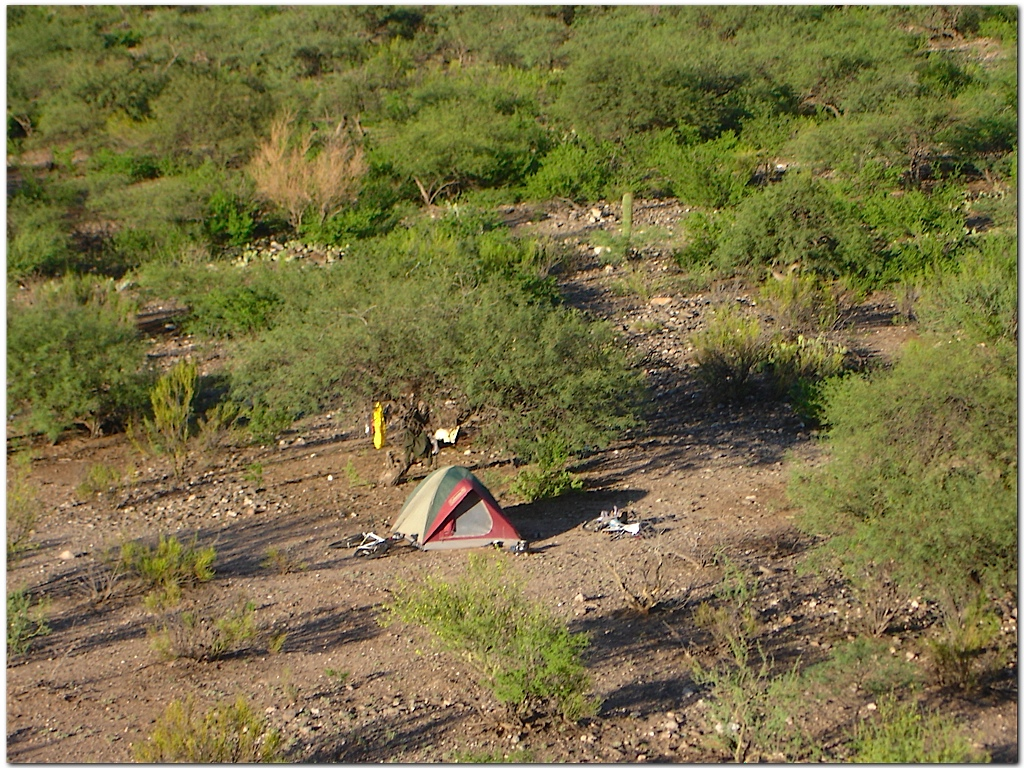
\includegraphics[width=300px]{images/DSC0123.JPG}
\textsc{\\``Camping libre.''}
\end{center}

\subsection*{18 de Enero -- Cafayate}

Desayunamos sobre el morro, observando tanto a las ruinas como a la ruta
mientras sub'ia el sol. Preparamos las alforjas para seguir a Cafayate. Ya en
camino, pasamos varios r'ios que atraviesan la ruta. Cruz'abamos Colalao del
Valle cuando decidimos parar a almorzar en su hermosa plaza central. Compramos
mont'on de verduras para armar una suculenta ensalada de todo, con condimentos
prestados por un due\~no de casa.

Pretend'iamos pasar la siesta para evitar al gran sol, pero, inquietos como
siempre, decidimos seguir pasado un ratito. A las pocas cuadras encontramos a
dos grandes viajeros en bici, bajo la sombra de los 'arboles. El calificativo de
``grandes'' se lo dan la apariencia de extranjeros lejanos, las banderas sobre
las bicis, las alforjas atr'as y adelante y el bob (carrito con bolsos tirado
por la bici). Se trataba de norteamericanos que hablaban buen espa\~nol. Greg
viaja desde Alaska a Ushuaia en beneficio de una fundaci'on
(\texttt{http://www.ribbonofroad.com/}), y Tom, estudiante de Geograf'ia, se
prendi'o en Quito, Ecuador, al pedaleo. Charlando nos morimos de risa por dos
horas, hasta que dieron las 4pm y siguieron viaje. Contaban unos relatos
impresionantes, dif'icil de seleccionar, pero me interesa por ejemplo que en el
desierto boliviano tenian que mandar comida en jeeps a los paradores, porque en
ese momento eran 5 viajeros y las proveedur'ias, casi fantasmas asentadas sobre
un camino tur'istico abandonado, no ten'ian provisiones para todos. En una, el
due\~no, al ver que le compraban literalmente todo por 100 o 200 soles, les dijo
que con 200 m'as les dejaba el negocio. \textexclamdown Embolado de vivir ah'i,
solo, cruzando a algun que otro loco dolarizado! Les vend'ia su lugar por poco
m'as que su mercader'ia. Muchas otras historias, como se imaginar'an; por la
onda le sugerimos al compa\~nero de Greg que conozca El Mollar.
``\textexclamdown Buen viaje!", y a la ruta en sentidos opuestos.

Bajadas y subidas de por medio, llegamos a Cafayate, muy pintoresca ciudad,
donde paramos en un camping medio caro en busca de buenos ba\~nos y duchas. Y
hoy, descanso y a pasar el d'ia en la pileta, esperando a nuestro amigo y
compa\~nero Sergio, profesor de Educaci'on F'isica de la Universidad de La Plata
de unos 50 a\~nos, que viene un d'ia desfasado. Ma\~nana empezamos juntos la
ruta a Cachi, me cago todo porque hasta estos grandes viajeros en bici me dicen
que ``la 40'' no es cosa f'acil.

\subsection*{19 de Enero}

Hoy seguir'iamos hacia Cachi, pero Sergio, llegado ayer, nos tent'o de
quedarnos. \textexclamdown El loco viene muerto porque le exigimos que se apure!
Dice que le ment'i, que no es dif'icil la subida de Tucum'an, \textexclamdown
sino que es ``dificil'icima''! Salimos a cenar, y luego de esperar una hora una
pizza\ldots\ \textexclamdown terminamos comiendo dos lomos completos cada uno en
un kiosquito cercano! \textexclamdown Y no nos movemos! Como lo invitamos, ahora
nos quiere invitar al almuerzo, venimos aliment'andonos como pavo antes del d'ia
de acci'on de gracias.

No quiere tocar la bici, as'i que paseamos a pie por la ciudad. Hoy vamos en
auto a la Quebrada de las Conchas, veremos de qu'e se trata, para ma\~nana s'i
continuar por la serruchada y enripiada {\small RN}40; no hay quien nos
tire buena onda pero ya veremos qu'e nos depara. Estamos expectantes,
\textexclamdown creo que nos va a cansar y a gustar mucho!

Yo ven'ia con miedo porque mi bici no anda muy bien: la cadena giraba en falso.
Luego de visitar dos o tres bicicleter'ias que me mandaban a Salta Capital
(imposible), porque ac'a hay viejos pi\~nones a rosca y no a cassette, termin'e
en la casa de un corredor de bicis, que se di'o ma\~na y con un buen trabajo de
limpieza la dej'o nueva. Cobr'o una m'odica mano de obra, y me salv'o buena
parte del viaje. Profundamente agradecido.

\subsection*{24 de Enero -- Cachi}

En estos d'ias completamos el viaje desde Cafayate a Cachi, no por Salta Capital
sino por la m'itica para nosotros ``cuarenta'', algo completamente inolvidable.
Pasamos por cuatro pueblitos perdidos (San Carlos, Angastaco, Molinos y
Seclant'as) que, me animo a decir, son los lugares que con m'as exactitud y
cari\~no recuerdo. Si se viaja con 'animos de conocer cultura, estos puntos
perdidos y sin inter'es tur'istico son el centro y nudo del viaje.

La Ruta impacta, no pasaba un alma. Desde San Carlos casi comienza el ripio,
'este es un pueblo que recuerda (por pel'iculas, pues no conozco) a M'exico,
antiguo y hermoso. Almorzamos aqu'i media docena de riqu'isimas y pesadas
empanadas salte\~nas (salte\~nas porque tienen papa hervida). No s'e como mi
boca sobrevive sin quemarse. Pedimos por el ba\~no y, muy amablemente, nos
condujeron por un largo corredor al patio central y privado, donde estaba el
precario ba\~no de los cocineros, los due\~nos de casa. Qu'e simple y gran
atenci'on a las personas (aunque en este caso fu'eramos clientes).

Hasta Cachi el ripio continu'o como empez'o: serruchos, suelo un tanto arenoso,
y muchas curvas y desniveles. \textexclamdown Un camino para no aburrirse! Se
cansan las piernas, pero no mucho m'as que la espalda, los brazos y el cuello.
Cruzamos algunos vados embarrados, 'este es en verdad un viaje para la bici. Los
paisajes cambian cada 5~km, uno no puede cansarse de mirar, en toda direcci'on y
momento.

Sergio casi muere, lleg'o descompensado. Es que fue un d'ia muy duro entre el
viento en contra y la dif'icil ruta, pero la emoci'on de estar haciendo
exactamente lo que quer'iamos no nos permiti'o decaer. La noche nos sorprendi'o
en camino, luego de dos pinchazos (durante el viaje pinchamos incontables
c'amaras, debido al peso, estado del camino, y baja presi'on con que
err'oneamente las infl'abamos), y sin embargo con Eze no sent'iamos buen humor,
sino una muy concreta euforia: salimos de Pergamino buscando \emph{esto}. Un
cielo netamente estrellado, y la luna est'a creciendo aunque casi no existe.
Bajamos la Quebrada de las Flechas --zona del camino donde se aprecian
indescriptibles formas que la erosi'on le imprimi'o a las monta\~nas-- a tal
velocidad que no nos permitimos detenernos para tomar fotos. Son los caminos que
esper'abamos.

Cuando vimos el cartel del desv'io a Angastaco s'i que nos detuvimos y, mientras
el extenuado Sergio enfocaba en la plena oscuridad, con Ezequiel nos
acomod'abamos detr'as del cartel planeando hacerle alg'un otro chiste. Nuestras
risas no le provocaron sospechas, y cuando dispar'o el flash retrat'o grandes y
blancos no nuestros dientes, \textexclamdown sino nuestros respectivos traseros!
Le preguntamos si salimos con mala cara, y entre carcajadas volvimos a subir a
las bicis para completar el desv'io al pueblo.

Llegamos a Angastaco de noche cerrada, con mucho cansancio y altos 'animos. Es
un pueblo m'inimo, con un campamento, su plaza e iglesia, una lujosa hoster'ia,
y muy poco turismo. Aqu'i por segunda vez me sent'i forastero dentro de ``mi''
propio pa'is. Llegamos a las 22:30, y lo que nos un'ia a los lugare\~nos
(reunidos en esta noche de s'abado alrededor de la plaza principal) era
'unicamente el partido River-Boca, que se proyectaba en el barcito dos cuadras
m'as arriba. Y tambi'en, claro, sus atentas miradas hacia estos ruidosos
viajeros.

Comimos en el barcito un delicioso matambre tiernizado, y tomamos una buena
cerveza. Divertida charla, y a medianoche salimos a buscar campamento. Pedimos
ayuda a unos j'ovenes que tomaban cervezas en una puerta de casa, y nos
acompa\~naron caminando hasta donde viv'ia el cuidador del campamento, quien
descansaba apaciblemente pero le interrumpimos, pidiendo que nos acompa\~ne a
nuestros aposentos. Agradecimos mucho a los j'ovenes, quienes, con la misma
simpleza con que nos ayudaron, se despidieron y volvieron a su vereda. El
hombre nos abri'o unos particulares bungalows, donde descansamos luego de darnos
un potente ba\~no. Desde una ducha Sergio suspiraba en su cansancio como si
estuviera d'andose un ba\~no de inmersi'on, \textexclamdown lo imit'abamos
exagerando y las risas se escuchaban en todo el camping!

Dormimos muy bien, y al levantarnos jugamos un picadito con ni\~nos del lugar,
nos miran como si vini'eramos del planeta Saturno. Luego Ezequiel y yo seguimos
hacia Molinos, y Sergio se qued'o a hacer vida de paz en Angastaco, lavando ropa
y acomodando la bici, que se le rompe m'as que la m'ia.

\begin{center} 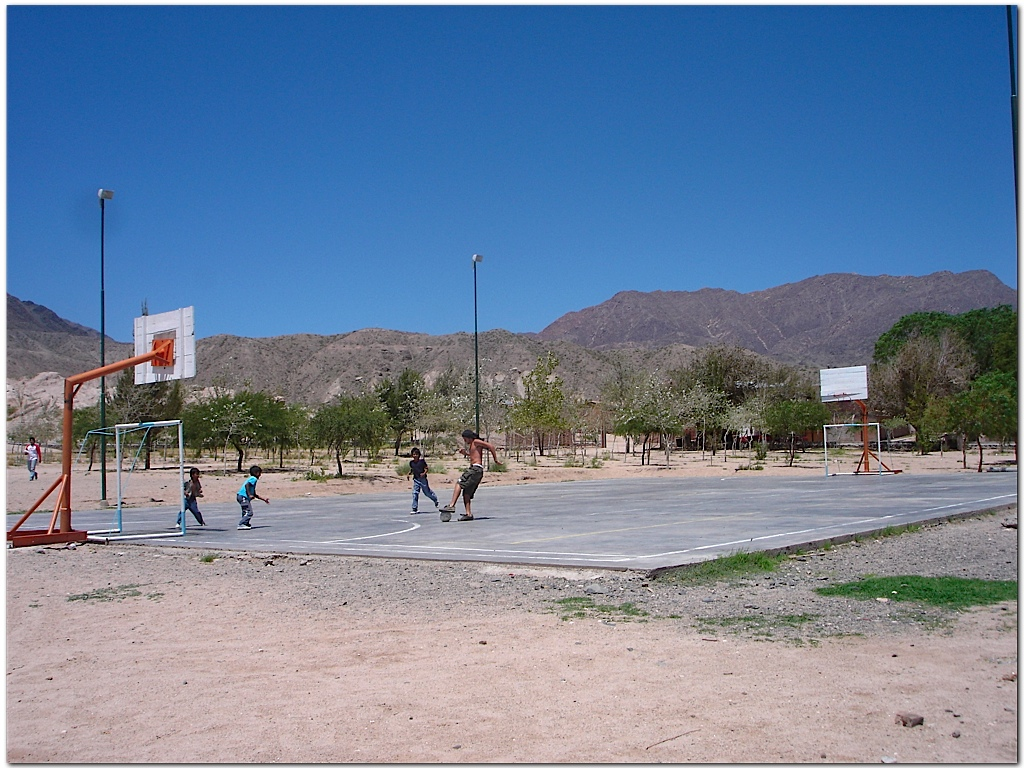
\includegraphics[width=300px]{images/DSC0194.jpg}
\textsc{\\F'utbol en Angastaco.} \end{center}

Camino a Molinos cruzamos tres turistas: uno era alem'an, de unos 27 a\~nos. Le
pregunt'e de d'onde es y me contest'o muy sonriente que viene de un pueblo
cercano a \emph{Hannover}.

\subparagraph{}\label{ssub:gottingen} --- \textexclamdown Mir'a vos! Yo viv'i
dos meses en G\"ottingen.\\ --- Bueno, \textexclamdown de ah'i soy!\\
\hangindent=1cm

Le pregunt'e por Gustav y por Axel, nombrando calles, y con cara de incr'edulo
me contestaba que no los conoc'ia. No dejaba de repetir ``\emph{it's
incredible}'', y la verdad que lo era.

El viaje fue muy sabroso, recorriendo una angosta ruta serpenteante, con tantas
cortas subidas como bajadas, precipicios a veces sin guardariel, entre aridez,
arboledas, cultivos regados por acequias, y monta\~nas. Pocos veh'iculos.
Encontramos a un lugare\~no sentado a la vera de la ruta, solo, vestido de
pantalones largos y camisa; y le ofrecimos agua seguros de su soledad, pero nos
indic'o su casa bajo la ruta. Esa familia viv'ia ah'i, incomprensible para
estos viajeros citadinos. Agradecido, nos dese'o un buen viaje. Yo no me detuve
hasta pocos kil'ometros antes de Molinos, donde par'e a esperar a mi
compa\~nero, sentado en un tronco frente a una casa de barro y paja.

Apoy'e la bici sobre la banquina y mir'e al camino, descansando. Se acercaron
dos ni\~nos de la casa interesados por mi viaje, y les empec'e a contar todo,
miraban con ojos grandes. Parece que esperaban con tanta ansiedad a Ezequiel
como yo, porque cuando lleg'o le demostraron m'as alegr'ia que yo mismo,
\textexclamdown se compenetraron con la historia!

Nos pasamos todo el atardecer jugando con otros hermanos y primos suyos, nos
contaron que ven'ian a esta casa a hornear el pan, nos ense\~naron la vista que
tienen desde arriba del cerro, y tomamos mont'on de fotos que nos hac'ian reir a
todos. Lo gracioso es que se sorprend'ian ante el paso de cada avi'on, y nos
escuchaban y miraban interesados, pero no les sorprend'ia la bicicleta m'as que
cualquier auto porque por esta ruta pasan, justamente, muchos viajeros de todo
tipo. Y como todos los ni\~nos de estas zonas, se alegraban tant'isimo de que
tuvi'eramos caramelos o galletitas dulces para compartir. Al bajar del cerro a
buscar pilas para la c'amara la madre sali'o t'imida de la casa, y nos regal'o
un pan reci'en sacado del horno, menos mal porque le com'ia un chico sino. Fue
hermoso. Despedirnos no fue tarea f'acil: cuando logr'abamos bajar a las
ni\~nitas --que apenas pod'ian caminar-- de las bicis e intent'abamos subir,
\textexclamdown se volv'ian a trepar! Agradecimientos, y a Molinos.

Molinos es un pueblo hermoso. Dej'e todos los bolsos en el camping y salimos a
comprar provisiones. \textexclamdown Era una moto! \emph{A fondo} por todo el
pueblo, me di cuenta de que tengo que limpiar los pobres frenos porque no
frenaba tanto como aceleraba. Me acostumbr'e al equipaje, y me vuelvo a sentir
como andaba en la secundaria: completamente liviano.

Al llegar al camping con las provisiones encontramos a los mismos chicos del
atardecer, viven por ah'i. Un poco vergonzosos, nos pidieron las bicis, y en
cuanto escucharon la primer letra del ``s'i'', se subieron y empezaron a hacer
carreritas en la calle de entrada del camping, se mor'ian de risa y no lo
pod'ian creer. Comieron de nuestra polenta, y se fueron a dormir cuando los
echamos; tambi'en nos 'ibamos a dormir.

A la ma\~nana hicimos una caminata larga por todo Molinos con un gu'ia del
lugar, muy buena. Conoc'i la tumba de quien descuartiz'o a Tupac Amar'u; el
antiguo hostal es de un descendiente directo de este espa\~nol de apellido
Isasmendi, quien vive ahora en Salta.

Ten'iamos dos caminos a Seclant'as, el 'ultimo de esta seguidilla de
tradicionales pueblos: el largo y el corto, el ``f'acil'' y el ``duro". Elegimos
el corto y dif'icil por la emoci'on de la bajada, y la disfrutamos; pero los
10~km de constante subida se hicieron largos, as'i que preferimos el otro, con
curvas y desniveles m'as constantes.

Telares y tapices por doquier, paramos en la casa del primer telar que vimos y
quer'iamos charlar con una vieja, pero no nos daba bolilla. Nos empezamos a
asustar: se acercaba sin emitir un sonido, y casi ni nos miraba\ldots\
\textexclamdown y es que era ciega y sorda! Nos escuch'o el hijo y nos explic'o,
casi morimos de un espasmo hasta ese momento.

Llegamos al camping, su due\~na y los dem'as acampantes nos trataron tan
amigablemente como cualquier viejo amigo. Aqu'i vimos por primera vez a una
norte\~na vestida t'ipicamente, y ella se sorprendi'o tanto de nuestra actitud
de pretender tomarle una foto, como nosotros de su vestimenta y de su caminata
con pesadas bolsas, a pesar de la avanzada edad.

Conocimos el cementerio, es t'etrico. El peor cementerio que conoc'i es el de
Seclant'as, peor a'un que el abandonado de Manuel Ocampo, cercano a Pergamino.
Sin planificaciones, atestado; uno entra y se choca dos tumbas, no hay caminos,
se anda por encima de ellas, los nichos son una desprolijidad\ldots\ desolador.
Se puede entrar a dos mausoleos de poderosas familias sin necesidad de entrar al
cementerio: est'an al costado y separados, y se ven a'un m'as que la propia
iglesia. Muy raro.\\

La distancia corta que recorrimos este d'ia permiti'o que Sergio nos alcance al
otro d'ia, as'i que, luego de nuestra noche en Seclant'as, salimos juntos hacia
Cachi. Recorrimos la ruta de los Artesanos, donde conocimos --entre otros tantos
(inhibidos como muy abiertos)-- al Tero Guzm'an justo en el d'ia de su
cumplea\~nos n'umero 77, el 23 de Enero. Le hizo ponchos a Juan Pablo II, Lula
da Silva, los Chalchaleros, y contando. Ya est'a un poco viejo para el trabajo
as'i que tiene a los nietos de ac'a para all'a. Le compr'e un cinto para mis
bermudas que queda de diez. Paramos en otros tres telares, y pinchamos otras dos
cubiertas adem'as de cambiar un cable cortado, por lo que la noche nos volvi'o a
sorprender.

Al atardecer, unos lugare\~nos de San Jos'e hab'ian armado una canchita de
f'utbol a lo largo de la ruta con rocas, \textexclamdown qu'e bueno! Tuvimos que
interrumpir su picadito: ``\textexclamdown perd'on que nos metamos en el campo
de juego, muchachos!'', nos re'iamos todos.

Nos rodeaba una violenta tormenta el'ectrica que por suerte no se posaba arriba
nuestro. Pedalear esos serruchos de la ruta, en medio de aquellas constantemente
iluminadas nubes de la noche, fue emocionante, aunque yo estaba asustado entre
la inminente tormenta, la oscuridad y los perros que a veces nos persegu'ian
ladrando.

\begin{center} 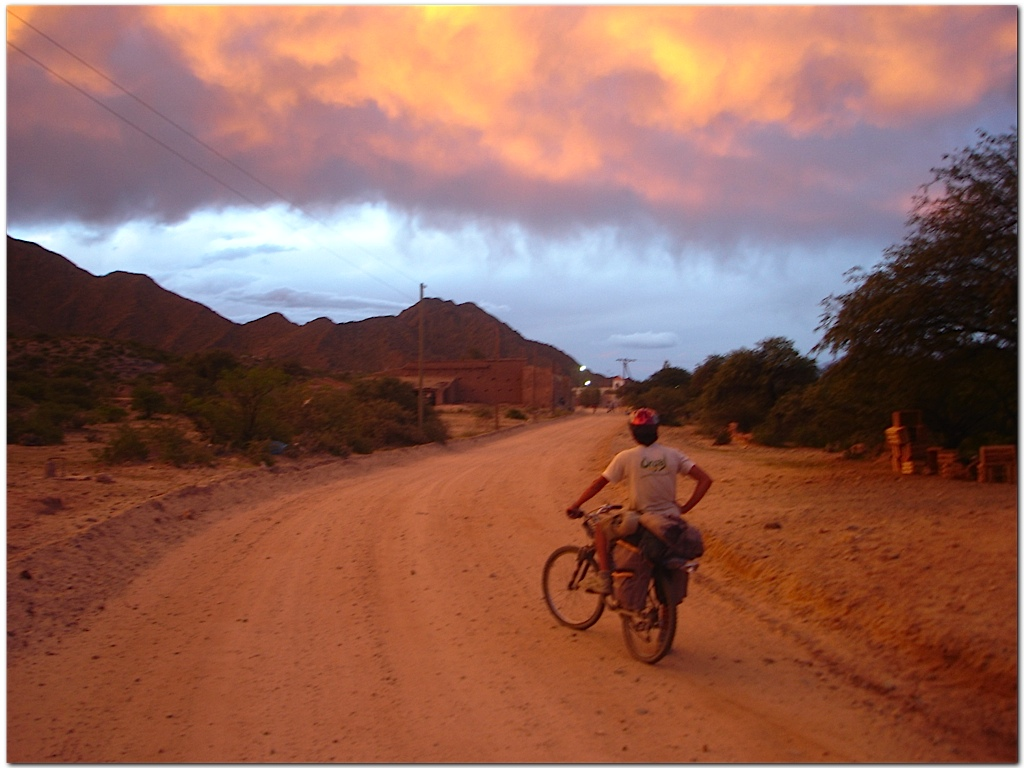
\includegraphics[width=300px]{images/DSC0296.jpg}
\textsc{\\Entrando a San Jos'e, bajo nubes po'eticas o infernales.}
\end{center}

La llegada a Cachi signific'o para mi un gran alivio. Bajamos por una de sus
calles hasta la plaza central, donde ahora nos esperaba Sergio, quien hab'ia
llegado directo por la 40 (sin artesanos: desviarse implicaba la noche en el
camino). Nos indicaron un hermoso comedor, donde ofrec'ian buenos y r'apidos
lomos, y mientras los disfrut'abamos se desat'o la instant'anea tormenta de
verano: lluvia a baldazos y unos rayos y truenos que hac'ian temblar la tierra;
nunca los escuch'e tan fuertes como en el Norte. Agradecidos de que no nos
sorprendiera en el medio de la ruta, terminamos el lomo y la tormenta de verano
pas'o, ahora se ve'ian las estrellas. Impredecible.

Bonito camping y buen descanso, nos tomamos un d'ia para recorrer esta
hermos'isima ciudad colonial, respirar, enviar noticias, tomar un aperitivo, y
las cosas que se hacen cuando uno se baja de la bicicleta. Toda la gente de lo
mejor, de diez. Los precios, norte\~nos, hasta llegar a Cachi que tiene ruta
pavimentada desde Salta.

\section{Pedaleando por las nubes, el Abra del Acay}

\subsection*{28 de Enero -- Al Abra del Acay}

Hoy nos separamos de Sergio en Payogasta, cerquita de Cachi: su viaje culminaba
en Salta bajando por la Cuesta del Obispo, pero el nuestro continuaba al Norte
por la 40. A la sombra de un gran 'arbol nos desped'iamos con una interminable
cola de chistes, hasta una vieja espectadora sonre'ia. Una canilla solitaria y
muy oportuna nos provey'o de agua. Lo vimos alejarse por el asfalto, y nosotros
continuamos en sentido contrario, luego de asegurar que se tratara de nuestra
ruta preguntando a la entretenida mujer.

Estamos expectantes porque nos acercamos al Abra del Acay, el punto m'as alto de
nuestras rutas Nacionales, que alcanza casi 5000 msnm. De lograr cruzarlo,
llegaremos bajando a San Antonio de los Cobres. Esper'abamos poco de esta ruta
desierta, sin embargo la altura, la inmensidad de las monta\~nas, y algunos
verdes valles se mostraron imponentes.

\begin{center} 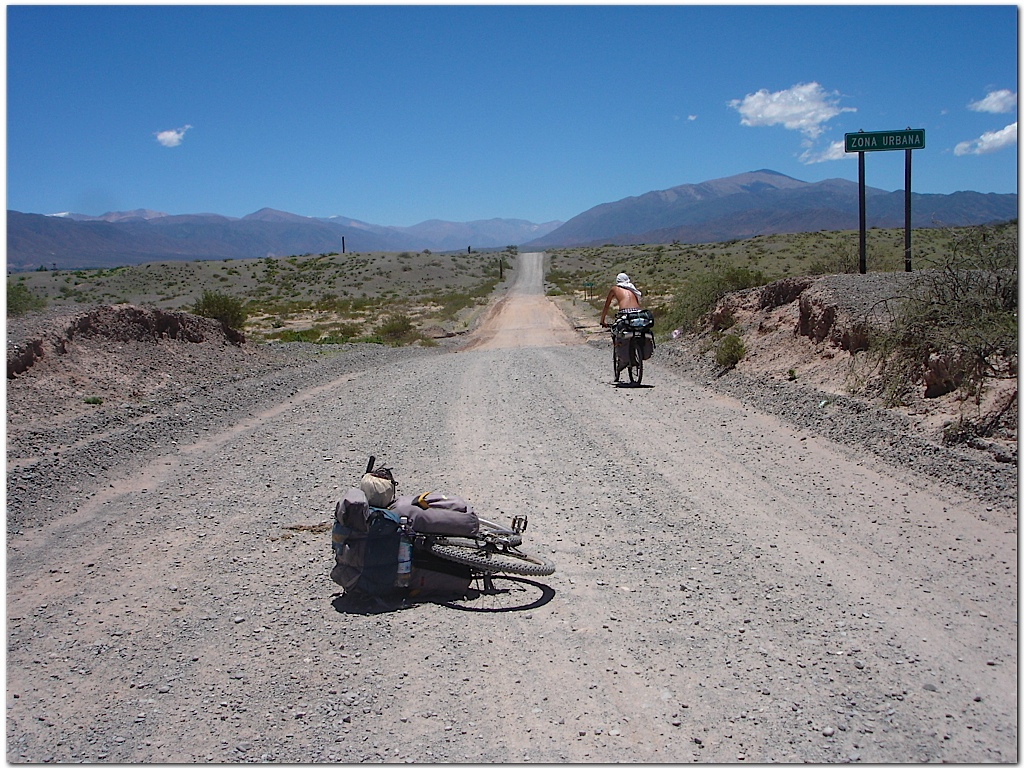
\includegraphics[width=300px]{images/DSC0311.jpg}
\textsc{\\``Zona urbana''. La bienvenida a la ruta desierta.} \end{center}

Pasamos el ``Pueblo Viejo'', y cruzamos por el camino a una muy avejentada mujer
que esperaba en la banquina. No pod'ia moverse ni hablar con facilidad, estaba
tan vestida que no entiendo c'omo no se deshidrataba del calor, y, sin embargo,
se mostraba muy interesada en charlar con nosotros, y no pod'ia borrar su
sonrisa. Ten'ia a su costado pesadas bolsas. Luego de una corta charla le
dejamos un paquete de galletitas dulces. Un encuentro irreal.

En todo el d'ia nos adelant'o un 'unico veh'iculo, y m'as tarde lo vimos volver
por donde ven'ia. Paramos a merendar sobre el camino, donde encontramos una
buena vista al r'io, dejando las bicicletas y bolsos desarmados sobre la
mism'isima Ruta 40. \textexclamdown Si pasaba alg'un veh'iculo, est'abamos
seguros, no tendr'ia m'as de dos ruedas!

Llegamos cansados y al atardecer al desv'io a La Poma, ciudad donde
dormir'iamos. \textexclamdown Esos 7~km (de desv'io) fueron los m'as largos de
todo el viaje! La Poma es un lindo y peque\~no poblado minero, asentado a los
pies de los volcanes extintos ``Gemelos", y habitado por pocos lugare\~nos y
otros tantos turistas (todos de aventura). Parece que aqu'i no se conoce turismo
``normal'', sino ciclistas, caminantes, y conductores de 4x4 ``extremos''; aqu'i
las alforjas no llaman la atenci'on.

Cenamos muy bien a las 8pm en un lugar que no ten'ia cartel, por esta zona
parece moneda corriente, este cyber tampoco tiene. Nos dimos un buen ba\~no
(que ansiaba desde hac'ia cuatro d'ias), y cenamos otra vez a medianoche, en la
posada, esta vez capeletinis.\\

Dormimos en camas con s'abanas, nos despertamos, y a desayunar y charlar con la
due\~na del lugar.

Nos cont'o sobre Damiana, una viejita que vive con su hija en ``La Negra
Muerta'', una casa construida 10~km antes del Abra. Nos aconsej'o firmemente que
paremos all'i y que no intentemos cruzar hoy, porque muy posiblemente nos
sorprenda la noche, y acampar en alturas parece tan peligroso como intentar
bajar a oscuras y debilitados; no hay chances. Nos dec'ia que Damiana estar'ia
encantada de recibir compa\~n'ia; y nosotros, encantados por conocerla,
aceptamos con ganas parar hoy all'i.

En La Poma hay gente un tanto reservada, \textexclamdown a algunos les costaba
responder a nuestras preguntas sobre el camino! Tambi'en los hay charletas, como
el due\~no de la proveedur'ia, al que no pod'iamos callar y nos retrasaba la
salida. \textexclamdown Miles de interesantes historias que contar sobre
viajeros y este particular cruce monta\~noso!

La ruta desde La Poma al Abra (y luego a San Antonio de los Cobres) es la que
imposibilita el tr'ansito de veh'iculos, con 4 cortes por r'ios y 2 por
derrumbes. Uno de los cortes por r'io ten'ia una ca'ida de 1 metro de alto.
\emph{Muy} divertido para atravesar con las bicis. A veces la ruta se pierde en
el lecho del r'io, y si uno lo sigue, unos cuantos metros m'as adelante vuelve a
encontrar la senda de ripio. La dificultad aqu'i era avanzar y no buscar el
camino, pues la ruta corre siempre por el valle exceptuando el Abra, donde se
unen las cadenas monta\~nosas y las atraviesa por arriba.

Los mojones, que deber'ian contar alrededor de 4600~km, presentaban inexplicable
y repentinamente ``escasos'' 1800~km, nos hac'ian sentir impotentemente perdidos
en medio de una lejana e inaccesible Cordillera. Soledad casi absoluta, excepto
por algunas cabras y su respectivo pastor.

No llegamos a lo de Damiana, armamos campamento al lado del r'io. Cenamos bien,
y dormimos ya sintiendo la falta de aire. Al levantarnos nos sorprendimos por la
escarcha que se form'o sobre la carpa. Dos locos estaban haciendo el camino a
pie, no se esperaban la ausencia de autos. Locos, \textexclamdown literalmente!
Nos encontraron esta ma\~nana, y desayunamos juntos. Les alivi'o nuestro t'e:
ven'ian muertos de fr'io y con los pies mojados (nosotros nos salvamos cruzando
los vados sobre las bicis).

Pretendimos conquistar el Abra esa siguiente jornada. Luego de mucho subir
encontramos una viejita muy parecida a una vela oscura derretida, bajaba
caminando y tejiendo de la monta\~na, rodeada de unos cuantos perritos. Le
pregunt'e si ella era Damiana (efectivamente ella era), y entonces pregunt'e si
est'abamos lejos de su casa, pero ``ahicito nom'as'', a la vuelta de la curva,
encontrar'iamos su casita. Irradiba una paz religiosa, mientras sus perritos no
nos dejaban de ladrar. Nos dec'ia sin dejar de tejer que est'abamos a tres horas
del Abra del Acay, y que lograr'iamos cruzar antes del atardecer, que
sigui'eramos. Pod'iamos parar en su casa, pero no encontrar'iamos a nadie.

\begin{center} 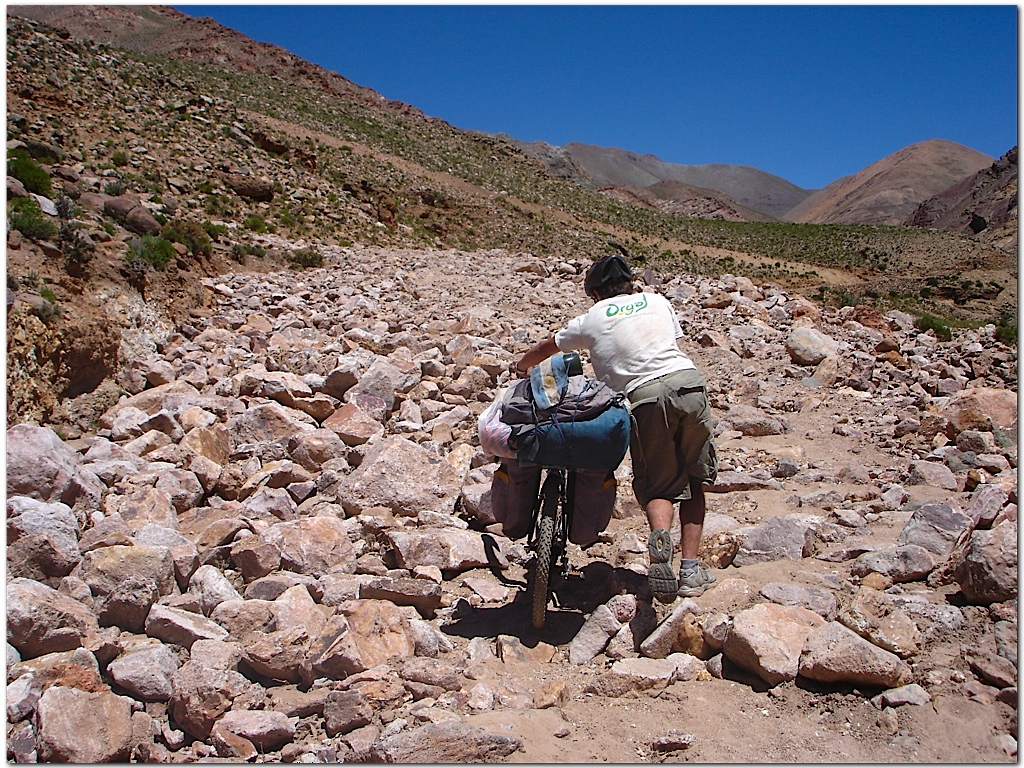
\includegraphics[width=300px]{images/DSC0369.jpg}
\textsc{\\Derrumbe sobre la Ruta 40.} \end{center}

Nos despedimos y continuamos el pedaleo. Pasamos por su casa, donde dejamos a la
vista nuestras galletitas para los dos caminantes, seguros de nuestro cruce.
Subimos mucho, nos cansamos moralmente: horas de subidas y curvas, paisajes
siempre iguales, cada vez m'as falta de aire, \textexclamdown el viento en
contra! Despu'es de cada curva esper'abamos ver la bajada, pero se demoraba
invariablemente. Continuamos sin que importe el paso de las horas: ten'iamos que
cruzar o volver para evitar el campamento en alturas.

Yo iba adelante, esperando poder anunciar la buena noticia a Ezequiel, y poder
levantar los 'animos. Y entonces, luego de una curva, lo vimos. Fue
desesperanzador. Estaba lejano, alt'isimo, subiendo una monta\~na por el camino
haciendo eses. Si cada veinte pasos --ni hablar de pedalear-- par'abamos a
tomar aire, probablemente llegar'iamos a medianoche, o ni lo lograr'iamos.
Desanimados, nos tiramos en la banquina. Abr'i una lata de carne y empec'e a
comer, no era agradable pero estaba hambriento. Ezequiel, asqueado, prefer'ia
evitarlo. Lo obligu'e a comer: ``Eze, uno de los s'intomas del apunamiento es
falta de hambre, justamente cuando m'as lo necesit'as. Comelo igual, dale''.
Pero lo vomit'o, sinti'endose cada vez peor. Me empec'e a desesperar:
\textquestiondown qu'e hacer? Somos inexpertos, \textquestiondown qu'e se hace
en estos casos? \textquestiondown Dormir en las alturas? \textquestiondown
Seguir, para poder luego bajar a San Antonio y comer a los m'as amigables
3700msnm? \textquestiondown Volver por donde vinimos, volver a La Poma? Ya no
quedaba suficiente agua y alimentos para alargar el viaje.

Durante esos pensamientos bajaban dos espa\~noles en bicicleta, reci'en hab'ian
cruzado en sentido inverso. Nos confirmaron que no llegar'iamos antes de la
fr'ia noche, restaban a'un 5~km. Aunque lleg'aramos, no ten'ia sentido describir
semejante bajada en las penumbras; deb'iamos hacerlo bajo el sol. Describimos el
camino de bajada que les esperaba, y nos dejaron un poco de agua, necesaria y
salvadora. Agradecimos, y siguieron bajando velozmente.

Intentaba preguntar a Ezequiel qu'e prefer'ia, pero le costaba pensar y
responder. Se sent'ia borracho, mareado al cerrar los ojos y con movimientos
poco exactos. Decid'i bajar un tramo, hasta alguna cueva formada por la
monta\~na donde armar la carpa y dormir. Si nos despert'abamos sinti'endonos
peor, volver'iamos sobre nuestra huella, y en caso contrario, la siguiente
ma\~nana seguir'iamos. Volvimos un par de kil'ometros, yo sent'ia miedo. En una
curva de 180$^\circ$ de unos caracoles que describ'ia el camino, contra la pared
de la monta\~na, armamos precariamente la carpa. Me acost'e en la bolsa de
dormir, vestido, pensando en que hab'iamos regalado provisiones seguros de
nuestra cena en San Antonio, pero nos tocaba este imprevisto cambio de planes. A
pesar de los minutos que transcurr'ian de descanso f'isico (pero no mental), mi
coraz'on no se calmaba, sent'ia taquicardia estando completamente quieto. Una
sensaci'on totalmente nueva e inquietante. Me asustaba el hambre y apunamiento,
lo que nos esperar'ia en el largo d'ia de ma\~nana, c'omo se sentir'ia Ezequiel
y yo, qu'e desayunar'iamos (sin hablar del est'omago vac'io de mi
compa\~nero).

Dormimos bien, a pesar del muy irregular y duro suelo rocoso. Nos despertamos a
las 8 de la ma\~nana al calor del sol. Abrimos la carpa y salimos, a'un
atontados por el profundo sue\~no. La sorpresa fue grande al vernos en medio
de ese imponente paisaje, peque\~nitos, luego de haber subido los caracoles que
se ve'ian hacia abajo, por subir los que nos esperaban adelante, y al costado
del profundo valle por donde bajaba un a'un peque\~no curso de agua, que
despu'es crec'ia. Levantarse as'i en el medio de la nada, pero de esos Paisajes,
es algo que no se puede describir. \textexclamdown Una sensaci'on moment'anea y
muy intensa!

Nos sent'iamos un tanto mejor f'isicamente, por buena suerte. Desayunamos leche
en polvo con la no mucha agua que quedaba. Mientras Eze terminaba con su
equipaje me recost'e sobre una roca, cerrar los ojos me acercaba casi
instant'aneamente al mundo de los sue\~nos. Y encaramos los 7~km que faltaban a
las 9:15 de la ma\~nana. Se sucedieron horas de profundo desgaste f'isico y
psicol'ogico, y sorpresa por nuestro ininterrumpidamente acelerado coraz'on. Sin
embargo, ahora pod'iamos ver desde arriba a las cadenas monta\~nosas que antes
rode'abamos subiendo impotentemente, y al pasarlas con la mirada pod'iamos ver
las distintas cadenas que se suced'ian. Luego de muchas horas de tener la vista
interrumpida por paredes, uno puede observar desde arriba a esa monta\~na que lo
encerraba y a las que le siguen, una sensaci'on enorme dentro del siempre
presente sentimiento de peque\~nez.

\begin{center} 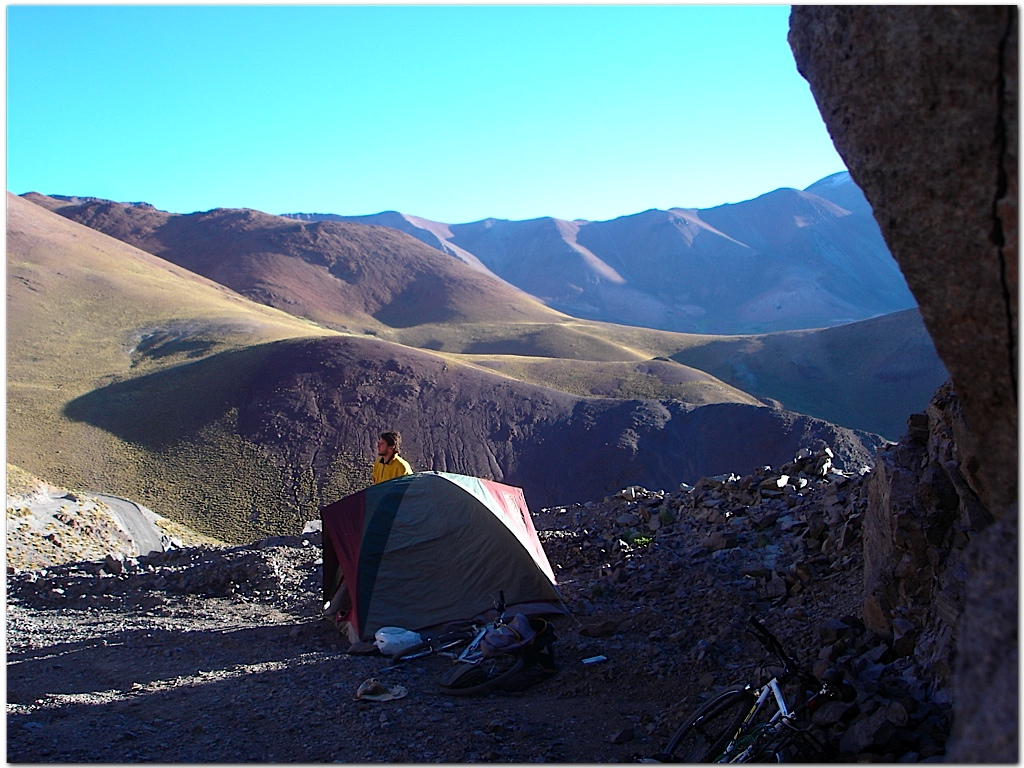
\includegraphics[width=300px]{images/DSC0375.JPG}
\textsc{\\Amanecer en el camino.} \end{center}

La otra sensaci'on que nos acompa\~naba ya fue descripta, pero intentar'e
transmitir la monoton'ia: uno sube las ``zetas'', sabiendo que luego de la curva
llega a la meta. Pero no, luego de la curva hay otra recta en subida, otra curva
m'as, y paisaje invisible desde esa perspectiva. Entonces se resigna, sigue con
la cabeza gacha, mirando hacia atr'as, o adelante seg'un el 'animo, llega la
curva, se da vuelta ansioso por ver el (\textexclamdown por fin!) Abra, pero no:
existe una nueva recta de iguales caracter'isticas. Los latidos se sienten en
todo el cuerpo. El sol abrasa. \textexclamdown Cu'anas subidas restan, Dios! Es
como si nunca se terminara, es como el juego ``viboritas'' en que la situaci'on
nunca mejora sino que empeora, a pesar de todas las frutitas que uno comi'o.
Pero lleg'o el momento en que no se ve'ia nada m'as que el cielo, y entonces era
seguro que ser'ia la 'ultima subida. Yo se que no pod'ia m'as, se que no ten'ia
energ'ias, pero se tambi'en que aceler'e imparablemente, hasta llegar a
comprobarlo. Y lo comprob'e. \textexclamdown Y hab'ia llegado! ``\textexclamdown
\textexclamdown {\small EZEQUIEL, LLEGAMOS}!!'' No m'as fr'io,
no m'as hambre, no m'as sed, no m'as cansancio. Euforia. Los Gemelos estaban
casi a nuestra altura. El camino se ve'ia desde arriba serpentear en ambos
sentidos. Era la cresta de la ola, el l'imite geogr'afico que podr'ia impedir
llegar a nuestro objetivo; era el inicio de nuestra Quebrada de Humahuaca.

Ezequiel estaba a dos curvas de distancia hacia abajo, unos 500 m. En un momento
de peligrosa confianza baj'e, no por el camino sino cort'andolo por la
monta\~na, para contarle, emocionado, que all'i mismo se encontraba el Abra, con
todos sus carteles, vistas y pompas. Hac'ia cinco minutos no serv'ia ni para
acostarme a mirar el cielo sin quedarme dormido, y ahora bajaba a ayudarlo a
empujar su bicicleta hasta el Abra; el estado emocional es tanto o m'as
importante que el f'isico, no se necesitan pruebas. Ezequiel tambi'en se
emocion'o y gan'o en energ'ias y voluntad, pero a'un se sent'ia mal
f'isicamente. Yo sub'i sin parar su bicicleta --que en estas altitudes es m'as
bien un obst'aculo-- hasta lograr posicionarla al lado de la m'ia, y lograr
``la foto'', algo incomprensible teniendo en cuenta que par'abamos a tomar aire
cada 100 metros o menos de caminata. Yo saqu'e dos fotos tontas como siempre (mi
talento fotogr'afico es cercano a nulo), y mi amigo, encargado de este aspecto,
de suerte que quiso acomodar la c'amara sobre alguna piedra para que nos
retrat'aramos juntos. Ni importaban las bicicletas. Lo 'unico que quer'iamos
luego de aquella foto de forzada pero muy alegre sonrisa, era bajar a San
Antonio, respirar, y volver a saciar nuestros vac'ios est'omagos. Debilita, la
altura, no es redundante el dato: como bichos de ciudad pampeana no lo
entend'iamos. Julio Godoy en su libro relata que en su primer gran cumbre
sinti'o\ldots\ humildad. No fue euforia, no fue orgullo, sino llana humildad
ante la enormidad que lo rodeaba.

Transitar esos 7~km nos llev'o 4 horas, muchas paradas hasta calmar pulsaciones.
\textexclamdown Los corazones hicieron m'as fuerza que las piernas!

Paisajes fenomenales, curvas, ripio, arena\ldots\ la bajada no permit'ia
aburrimiento. Si bien era muy divertido y extra\~no no pedalear para avanzar, no
era f'acil, avanzando un tanto mareados, r'apido sobre un suelo tan irregular.
Cuando llegamos a la recta (de la Nacional 40, no se lo pierdan) \textexclamdown
ten'ia tantos vados, canaletas, arena y piedras de todos los tama\~nos,
\textexclamdown que mantener el equilibrio sobre las r'apidas bicis se hac'ia
dif'icil! Cruzaban llamas a veces, se las ve'ia correr por los valles desde
arriba en el camino.

Luego de otra larga recta con fuerte viento en contra (como todos estos d'ias,
el viento) llegamos a San Antonio de los Cobres en estado de inanici'on: hac'ia
dos d'ias, casi, que no com'iamos, con todo el esfuerzo que hicimos. A las 5 de
la tarde entramos en un restaurant sin cartel a pedir comida.

\subparagraph{}\label{ssub:comerAhora} --- \textquestiondown Comida?
\textquestiondown Pero ahora? \\ --- \textexclamdown S'i! \textexclamdown
\textexclamdown Como si fuera un almuerzo o cena!!\\ \hangindent=1cm

As'i que comimos de entrada una suculenta pizza, para dejar lugar al plato
principal: una milanesa napolitana con ensalada. Dos gaseosas\ldots\
\textexclamdown comimos como si fu'eramos cuatro! ``Gracias por la merienda", le
dijimos a la buena mujer, y a instalarnos en una suerte de hostal vac'io, donde
dejaron la calefa puesta. Ba\~naditos, al cyber, postres dulces, \textexclamdown
y a dormir!

Hermosa gente encontramos por la 40. S'olo lugare\~nos, y otros dos mochileros.
\emph{Nadie} m'as. No llegamos a conocer a un ciclista ingl'es que iba un d'ia
m'as adelante que nosotros (nos llev'o un d'ia m'as de lo pensado el gran
trayecto).

\textexclamdown Bueno, eso ser'a todo, resumid'isimo aunque no lo crean! El Abra
ser'a algo dif'icil de olvidar. Lo comparaba con el cruce de la cordillera por
Mendoza, s'olo que much'isimo m'as dif'icil (ripio, arena, viento, falta de
aire, de gente y de provisiones). Y, claro, tambi'en \emph{hermos'isimo}. Las
monta\~nas que 'ibamos rodeando se iban viendo desde arriba a medida que
ascend'iamos. Se siente.

Ma\~nana, colectivo a Purmamarca: a Eze no le dan los d'ias para pedalear por
las Salinas y tambi'en llegar a Iruya, que creemos prioritario.

\textexclamdown Un abrazo enorme a todos!

Tute.

\section{Vuelven las vacaciones: hacia la Quebrada}

\subsection*{1 de Febrero}

\textexclamdown Hola, familia y amigos! \textquestiondown C'omo andan?

Llegamos a San Antonio muy cansados y hambrientos, por fin bastante aire y
suficientes alimentos. Dormimos en su oficina tur'istica a'un no oficial, y
desde aqu'i avanzar'iamos por Pozo Largo y Tres Morros, a trav'es de las Salinas
Grandes, para bajar por la Cuesta del Lip'an a Purmamarca: la Quebrada. Para
ello deb'iamos quedarnos descansando otro d'ia, y viajar a pedal otros tres,
pero las cuentas para llegar a principios de Febrero ya no daban, por lo que
aquella misma ma\~nana tomamos un colectivo a Purmamarca, con transbordo de
pocas horas en Salta (hermosa, verdaderamente). La ruta a Salta, incre'ible, y
luego nos tocaba la selv'atica ruta 9. El d'ia de descanso avanz'abamos,
\textexclamdown extra\~no!

Purmamarca es un pueblito hermoso, es famoso su cerro de los 7 colores, que se
debe llamar as'i por tener todos los colores que en la Quebrada abundan pero en
ese 'unico accidente geogr'afico. Sorprende de este poblado la uni'on de turismo
familiar y mochilero, siempre separados kilom'etricamente, pero ahora casi
compartiendo los mismos lugares. Descansamos dos d'ias: primero viajando en
colectivo, luego recorriendo los alrededores: pues no nos quisimos perder, a
pesar del cambio de ruta, las Salinas Grandes, y tomamos un colectivo para
conocerlas. La Cuesta del Lip'an fue maravillosa: el camino sube 2000 metros en
pocos~km, para bajar luego desde esos 4000 a las Salinas, a unos 3000 msnm.
Incontables curvas pavimentadas, en buen declive, y en ese marco monta\~noso.
Bajarlas en bici era sin precio, pero de verdad no podr'iamos llegar a completar
el viaje, de hacerlo. Y las Salinas\ldots\ perder la vista en esa plana s'abana
blanca y encandilante, luego de semanas de monocrom'aticas monta\~nas, fue
m'agico.

Buen sol todos los d'ias. Buen camping, buena gente. Cenando toc'o un d'uo medio
candombero espectacular, con caj'on de percusi'on, guitarra, voces y muy, muy
buena onda. Alegr'ia.

Bici a Tilcara, 20~km de viento a favor y pavimento, no podemos creer lo poco
que nos llev'o. Paramos en Maimar'a, poca gente lugare\~na, interesados en el
viaje y muy simples y abiertos. Aqu'i, la Oficina Tur'istica, la Terminal de
Omnibus y el Registro Civil, comparten un mism'isimo edificio. Mientras hablaba
con pap'a por tel'efono luego de varios d'ias sin comunicaci'on, Ezequiel
charlaba sin parar con un ni\~no que bajaba por una calle en su bici; cuando yo
cortaba ellos se desped'ian con un fuerte abrazo. Le hab'ia dejado \$2 para que
puediera ba\~narse en la pileta del club municipal, un regalo perfecto para la
calurosa tarde. \textexclamdown Creo que la sonrisa de Eze era m'as grande que
la del chico!

La Quebrada de Humahuaca es como conocer en pocas horas distintos pa'ises,
\textexclamdown todo el tiempo cambia el paisaje! Un buen viaje: el decidido
viento Sur convirti'o las subidas en planicies. Tilcara es otro lindo pueblo,
luego de recorrerlo en bici las dejamos en alg'un campamento, y subimos a pie al
Pucar'a de Tilcara, ruinas ind'igenas con vista interminable a trav'es de la
Quebrada de Humahuaca, y adelante, hacia otro valle. Los Pucar'a pod'ian ver
acercarse personas a decenas de kil'ometros de distancia, pero no aprendimos
mucho m'as sobre su historia.

Y ma\~nana, a Humahuaca: unos 40~km de buen viento Sur. Los d'ias ya aprietan,
eso no est'a tan bueno, sin embargo vamos a llegar a Iruya si todo sigue como
viene, bien.

\textexclamdown Un abrazo grande a todos!

Tute.

\subsection*{2 de Febrero}

\textexclamdown Hola a todos! \textquestiondown C'omoandan? (De nuevo noanda la
barra espaciadora.)

Che, me invitaron por mail a unirme a un apag'on de 5 minutos para solidarizarme
con el calentamiento global. \textexclamdown No saben que nos estamos
solidarizando desde hace tres semanas! Cuando lleguemos vamos a prender y apagar
la luz como ``El N'aufrago''.

Es sensacional pedalear por lugares como Humahuaca. Las angostas callecitas de
piedra, grandes plazas, casas coloniales, y los grandes faroles antiguos del
centro hist'orico de Humahuaca nos cautivaron. Adem'as, llegamos el d'ia de la
Fiesta de la Virgen de la Candelaria, mitad cat'olica mitad pagana. No
esper'abamos combinar con ninguna de las fiestas norte\~nas, fue algo
inolvidable. Hab'ia diversos grupos musicales de los alrededores, todos tocando
m'usica andina con sus tambores, sicus y otros; dos ``leones'' dando la vuelta a
la plaza tirando fuegos de artificio; cientos de turistas mirando y escuchando
extasiados; y la iglesia tocando sus campanas en plena noche y madrugada. Fue
asombroso y bien divertido. De visitar la Quebrada, hay que visitar alguna de
sus fiestas regionales.

Hab'ia mucha gente. Los sicus sonaban met'alicos, como un carrito de
supermercado que chilla, no como aire en una ca\~na; raro. Tipo 1:00
interrumpi'o una repentina y potente tormenta de verano, pero como tal se alej'o
en breves minutos. Las celebraciones comenzaron de nuevo a las 6 de la
madrugada, mientras dorm'iamos pl'acidamente. La iglesia empez'o media hora de
campanadas, todo empezaba de nuevo, sin embargo seguimos durmiendo como
lechonazos.

Nos levantamos a duras penas a las 11am, desayunamos, compramos uvas a falta de
sand'ia para el camino, y a pedalear a Chaup'i Rodeo, a mitad de camino de
Iruya, unos 45~km. Ma\~nana estaremos llegando all'a si todo va bien. Estoy
ansioso y expectante.

Vamos encontrando gente de otros campings, todos vamos al mismo paso; lo empiezo
a sentir, claro, en la Quebrada y no por la 40.

Si bien ayer en la tarde me informaron de la inminente aunque impredecible
muerte de mi abuelo, y Ezequiel me acompa\~nar'ia de vuelta en caso de querer
estar en Pergamino cuanto antes, decid'i seguir a Iruya. 'El estaba enfermo
desde hac'ia tiempo, y tuve ocasi'on de despedirme antes de mi partida. El
intercambio de palabras que mantienen un viejo ya cercano a su muerte y un
joven, donde el primero eval'ua c'omo vivi'o y c'omo vivir, desde su peque\~na
o gran experiencia. Lo enorme es la irremediable humildad desde la que habla, no
importa, justamente, su grandeza o peque\~nez en la vida que llev'o. Eso, creo,
es lo que aporta valor a esos pensamientos.

Volviendo a Humahuaca, es una ciudad cuyo centro es espectacular, bien colonial;
aunque en las afueras se parece m'as a la ciudad de Tucum'an. Ac'a todos muy
abiertos: encontramos introvertidos o caraduras por el camino; \textexclamdown
no hay lugare\~nos ``t'ermino medio''!

Contentos, a ver c'omo nos tratan las piernas en nuestro segundo tramo de
subidas en ripio. Los paisajes, dicen, prometen. La bajada a Iruya, dicen, es la
mejor frutilla del postre que hayamos podido elegir. \textexclamdown No est'a
bueno esperar tanto de una cosa, pero as'i es como estoy!

\textexclamdown Un abrazo grande a todos! \textexclamdown Cuenten como andan!
Beso grande;

Tute.

\subsection*{3 de Febrero}

\textexclamdown Hola a todos! \textquestiondown C'omo andan?

Llev'abamos un buen viaje cuando a los 20~km, la tormenta que me tocaba los
talones me desesper'o, y entr'e en Hornaditas m'as nervioso de lo que deb'ia.
Para colmo era una enorme nube pasajera que a la media hora desapareci'o (aunque
hubo otras). Lleg'o Eze y pens'o en quedarse una horita a descansar, o ``lo que
queramos'', as'i que estando de acuerdo nos echamos bajo la copa de un gran
'arbol. Hornaditas es una comunidad aborigen, este era una suerte de centro
institucional, con canchita de f'utbol, iglesia, jard'in de infantes, y un
caser'io. Nunca nos levantamos para seguir.

Estamos mal, hay algo que sentimos y no sabemos si es por altura, luego de tres
semanas de aclimataci'on: cansancio extremo, dolor de cabeza, ganas de dormir y
dormir, y de no comer porque no podemos digerir. Descans'abamos bajo un hermoso
'arbol, cuando pas'o un t'imido lugare\~no a pie, lo saludamos y si contest'o lo
hizo muy bajito. El hombre, Beto, entr'o en el sal'on de la iglesia y se nos
vino la imagen de Uspallata: ``\textexclamdown en este viaje nos falta dormir en una iglesia!''
dec'ia Eze. Al salir le pedimos alojamiento, nos ofrec'ia un sucucho bien sucio.
Luego ofici'o de gu'ia tur'istico mostrando un tremendo mirador (los colores del
cielo, irreales), el card'on m'as viejo y grande de toda la Quebrada, y nos
dec'ia que el desv'io a Iruya no tiene cartel (\textexclamdown mentira!) y que
m'as vale llegar de d'ia (era el atardecer). Sin decirlo aceptamos no
seguir viaje, as'i que fuimos a arrear unas cabras y a divertirnos con un perro
que devolv'ia los cabezazos que 'estas le tiraban. Pasamos una buena tarde, se
hizo de noche, y nos permiti'o dormir en el sal'on de la iglesia, con olor a
vino por el festival del s'abado pasado. Buen'isimo, ni carpa armamos. (A
medianoche y desesperados, s'i, \textexclamdown malditos mosquitos!)

\begin{center}
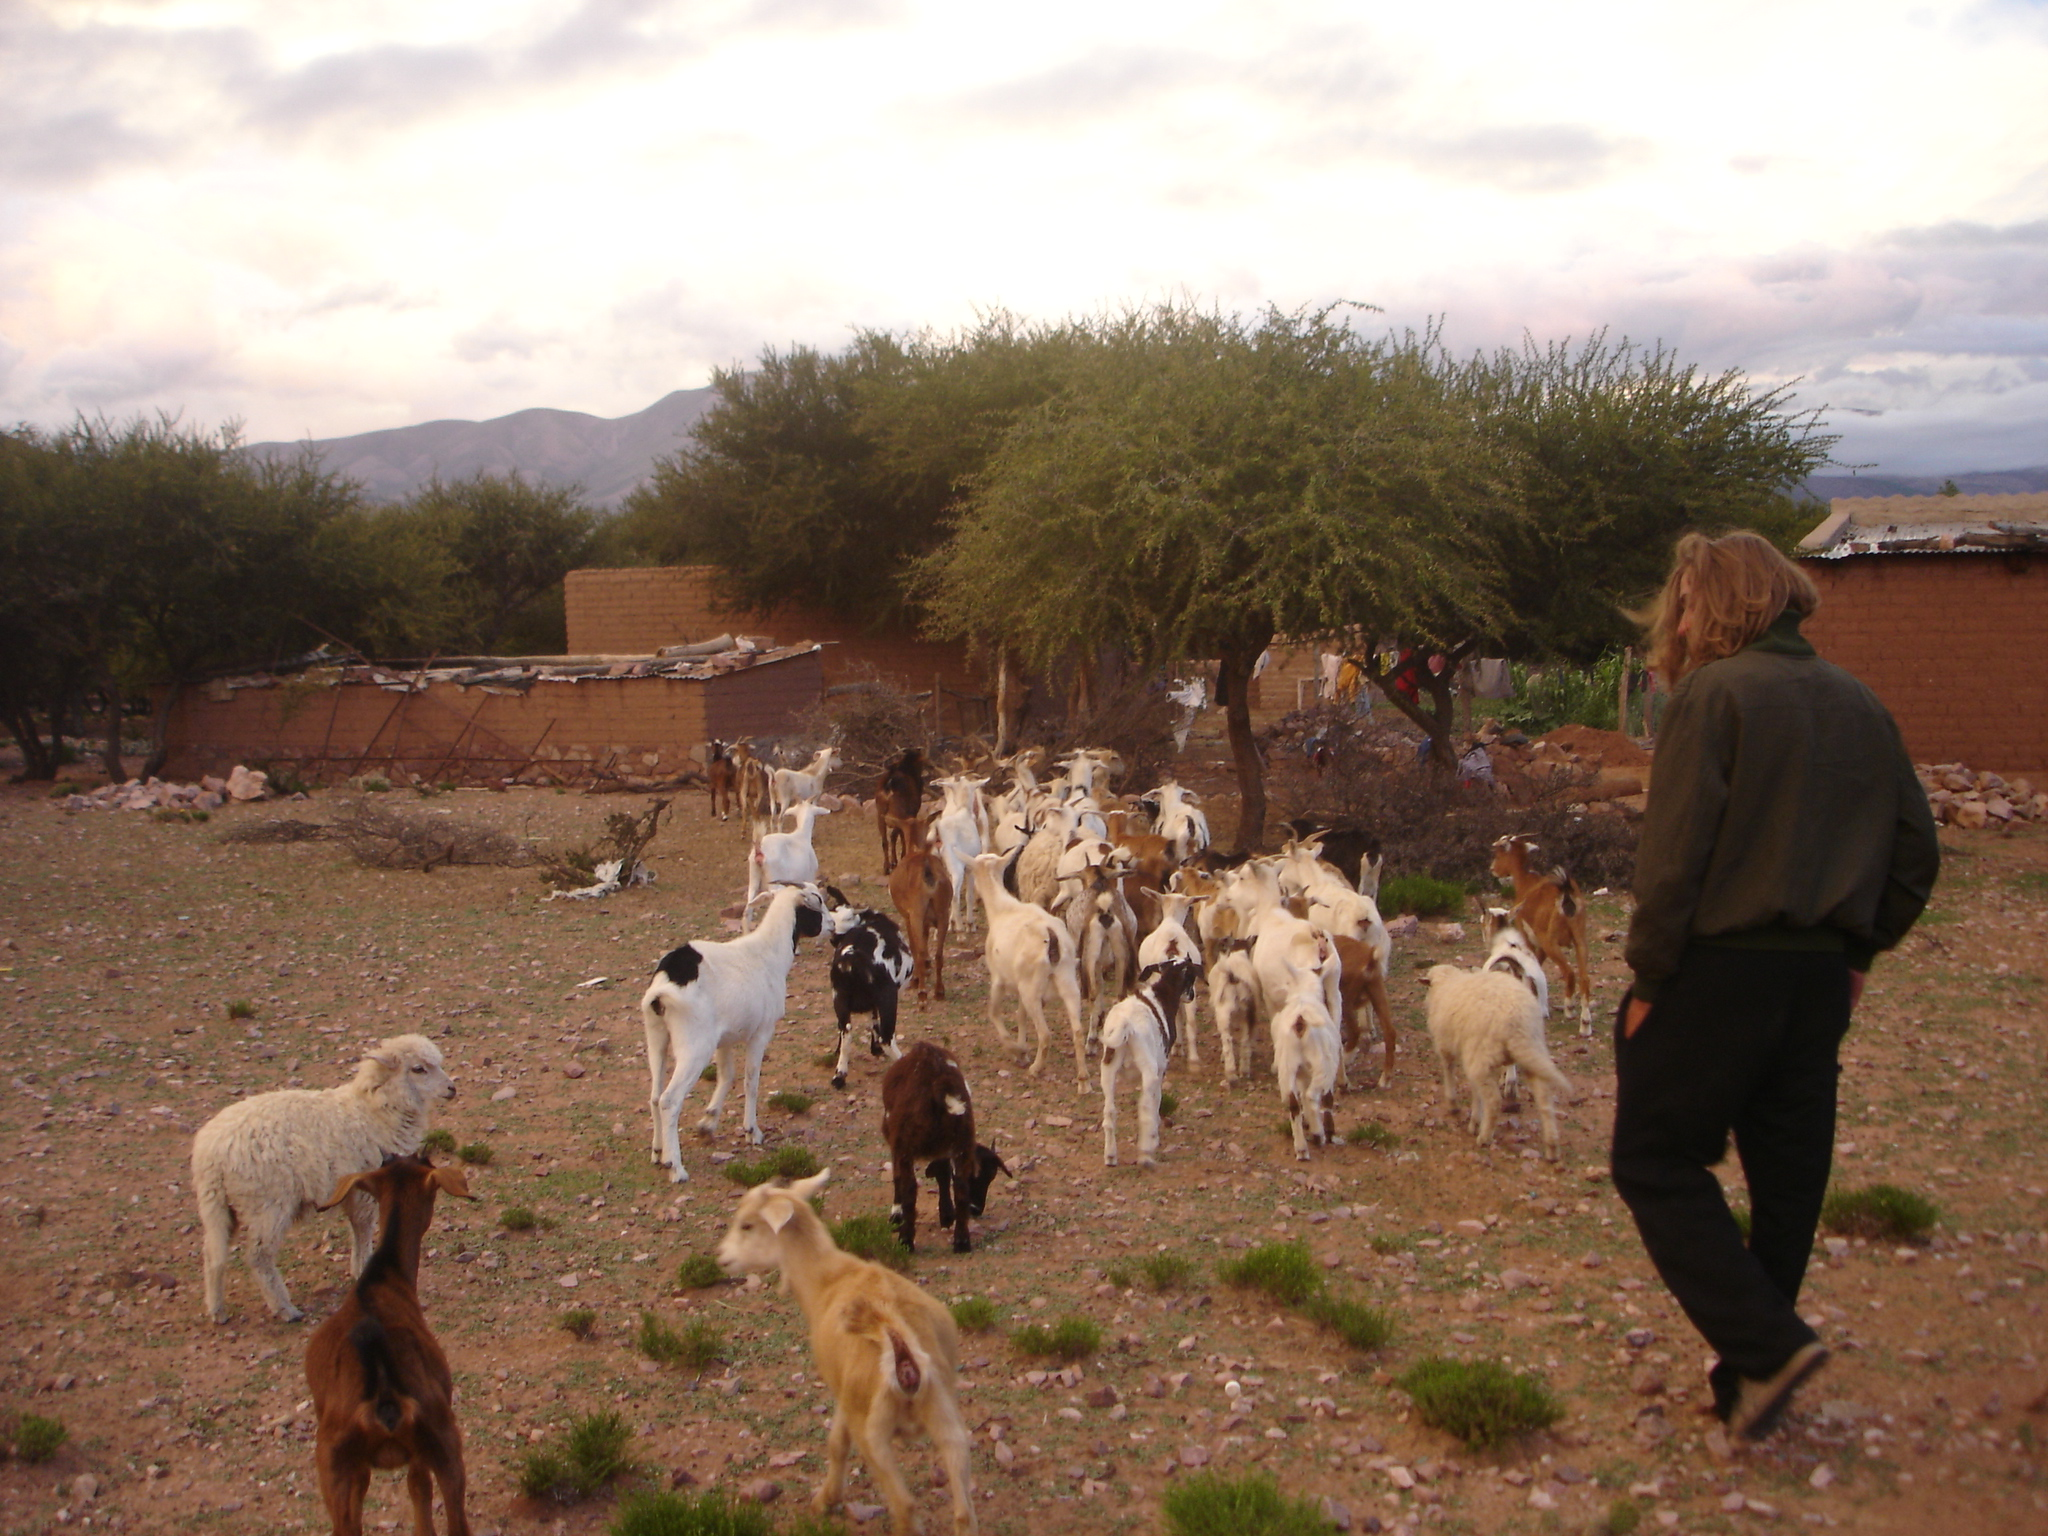
\includegraphics[width=300px]{images/DSC0446.JPG}
\textsc{\\D'ia de descanso.}
\end{center}

Cenamos poco arroz en el sal'on de la Iglesia que el muchacho nos prest'o, y ya
m'as en confianza, nos empez'o a contar de su vida. Beto es de Hornaditas, 26
a\~nos, soltero, m'as bueno que el pan lactal. Se encarga de muchas cosas, pero
oficialmente nos coment'o que de encender y apagar la bomba del agua todos los
d'ias. Pero por ejemplo, esas cabras no eran de 'el, sino del hermano, aunque lo
llamaba ``vecino''. Lo invitamos a un arroz tan rico como pudimos y, contaba que
un d'ia llegaron (es por desv'io, no es tan com'un la gente por aqu'i) dos
sacerdotes espa\~noles y le hicieron muchas preguntas que 'el contest'o con
buena predisposici'on. Tiempo despu'es les lleg'o la noticia de que la comunidad
de Hornaditas era beneficiaria de una ayuda econ'omica proveniente de no-se-qu'e
fundaci'on religiosa para que instalen la bomba de agua con su trabajo, y que
puedan dejar de llevarla en bidones de 5lts. Cumplieron tan bien que fueron
enviando m'as peticiones y se las fueron concediendo, as'i que con esa ayuda
concretaron otras cuantas obras. \textexclamdown Orgulloso el hombre de lo que
hab'ian logrado entre todos!

Un tipo muy interesante, simple, amigable y de personalidad humilde; escucha
atento las historias de todos los turistas que pasan, usualmente mochileros. No
pod'ia creer que nunca hayamos cruzado por Buenos Aires a famosos de la
televisi'on que 'el nombraba; le describimos c'omo es la Capital, comparando con
las extensiones de aquella ruta, ya que no pod'ia imaginarse la dimensi'on.
\textexclamdown Tantas personas! Tambi'en se sorprend'ia el buen hombre de que
no supi'eramos lavar ropa, ``\textexclamdown Mir'a esos cuellos!'' Claro, ese
lavarropas que nos acostumbra. Escuchaba atento el hombre, pero siempre para
conocer y de modo simple, agradable.

Luego de una charlita con 'el y una discusi'on entre nosotros decidimos tomar
los colectivos ``Mendoza'' hasta Iruya, o por lo menos al Abra del C'ondor, el
punto m'as alto del camino (4000 msnm) para hacer la bajada; ya que no nos
sentimos bien ni con ganas de hacer esa ruta de subida. Todav'ia ten'iamos que
arreglar una rueda pinchada. Nos acostamos a domir invitando a Beto al desayuno
de ma\~nana, aunque ten'iamos poca chocolatada y galletitas. Dejamos sonar el
despertador de las 7, y cuando lleg'o a las 8 se sorprendi'o de que a'un
durmi'eramos. 'El se volvi'o a Humahuaca dej'andonos desayunar, y nos sugiri'o
el colectivo de las 11. Nos levantamos, desayunamos poco, y lleg'o su hermano
mayor del festival de Humahuaca

Era un borracho que empez'o a relatar todos sus problemas, debilidades y ciertos
miedos, porque nos encontr'o amigables. Admiraba a Beto, y a mi me daban
l'astima sus muy bien aprendidos hijos. Uno, Alejandro, de unos 10 a\~nos, es el
que hace ah'i de gu'ia, y se lo notaba muy abierto, atento e interesado.
\textexclamdown Fuerte! Pero me daban l'astima por su padre, que no dej'o de
mostrarles cari\~no aunque hablaba demasiado. Mientras hablaba
seguimos organizando, descansando y nos despedimos para ir a buscar el cole.

Contentos por el rotundo cambio de planes y la gente conocida fuimos a esperar a
la banquina, un tanto nerviosos por si suben o no las bicis. Pasaron dos sin
parar haciendo se\~nas de que esper'aramos, y el tercero (van de a tres o
cuatro) par'o, as'i que las subimos. A'un nos dol'ia un poco la cabeza. Subimos
al ``Mendoza'', hermoso, de los de las publicidades de la pel'icula ``R'io
Arriba''. Le dijimos que vamos hasta el ``Abra del Condor'', no Iruya:
\textexclamdown subimos en cole y bajamos en bici! Nos permitimos la licencia.

Camino espectacular, charlando con un amigable neoyorquino jubilado, que
oportunamente se fue a otro asiento para seguir contemplando los paisajes en
silencio. Llegamos a esos 4000msnm, donde empezamos a bajar del techo las bicis.
Eso s'i que sorprendi'o al pasaje, no se esperaban que sigamos la bajada en la
bici. Todos nos deseaban suerte, una gran buena onda. ``\textexclamdown As'i
cualquiera anda en bici!'', y risas.

Ah'i, a unos 22~km de Iruya, abandonamos el colectivo para seguir en dos ruedas,
el pasaje y el conductor nos miraban sorprendidos mientras luch'abamos en el
techo para bajar las dos bicis.

Este camino es similar al de la bajada del Abra del Acay pero con buen viento,
muy divertido. A diferencia de otras bajadas que vivimos, tiene pendientes m'as
empinadas, y la bajada es ininterrumpida hasta Iruya. Tres veces llegamos a
velocidades peligrosas {\sl (adrenalina)}, y hasta en un declive saltamos con
bicis y bolsos, \textexclamdown fascinante! Llegu'e a unas ``eses'' que se
pod'ian cortar por una recta que las atravesaba por el medio. Me mand'e con una
gran sonrisa pero las m'as grandes piedras mordieron la rueda trasera, que se
desinfl'o en instantes. La cambi'e en instantes y segu'i bajando, con el
objetivo de alcanzar los colectivos. Los perdimos, el tema del equipaje llevaba
su tiempo y tuvimos que reorganizarlo porque se iba desarmando con el traqueteo.
Comparo este viaje con un rally: frenando la trasera para entrar mejor en las
``U''s, haciendo fuerza en el manubrio para que siguiera el camino que quer'ia;
rocas, piedras, canaletas, cursos de agua\ldots\ s'i, la bajada era fabulosa.
Necesito m'as fuerza en las manos.

Llegamos, vimos desde el camino aquel famoso campanario cuadrado y celeste de
Iruya, cerraba el incre'ible viaje y nos dieron ganas de cortar las cintas de la
llegada. En realidad, dos cuadras antes empezaba una intensa subida.
\textexclamdown Casi que llegamos caminando a nuestra meta final!
\textexclamdown Llegamos de suerte a'un pedaleando!

Iruya se asienta en la parte baja de la uni'on de tres valles, es decir que
est'a rodeado de altas, inmensas, paredes de piedra y tierra. Luego de caminar
todas sus calles (cansador, \textexclamdown no hay una cuadra plana!) fuimos a
descansar a una bella hoster'ia, cuatro cuadras m'as adelante (y arriba) que la
iglesia central. \textexclamdown Paramos dos veces a tomar aire camino a
nuestras camas!\\

Aqu'i pasaron cosas interesantes. Eze se intoxic'o no sabemos con qu'e, por
suerte justito al llegar a nuestra meta. El el'astico que sostiene todo mi
equipaje se cort'o dos veces\ldots\ \textexclamdown llegados a Iruya! Es decir
que ya pod'iamos volver tranquilos.

Recorrimos poco Iruya, no conocimos mucho. Nos perdimos una caminata por el r'io
hasta San Isidro que plane'abamos hacer. Caminar las calles del poblado no
llev'o demasiado tiempo, y la verdad es que ya ten'ia ganas de volver. Hoy
Domingo tomamos un cole de vuelta a Humahuaca. Y desde aqu'i combinar'iamos con
Salta y Pergamino, pero hay un colectivo que sale derecho de Humahuaca a
Rosario, y como ya estaba ansioso, lo tomamos. Lo 'unico que me queda en el
tintero, y no es poca cosa, es conocer mejor Salta capital. Pero es lo 'unico
porque de la ruta, \textexclamdown todo concretado! Contentos.

En el viaje a nuestras Pampas comenzamos a ver verde de nuevo; planicies, y
'arboles\ldots\ se extra\~naban. \textexclamdown Ya no vemos piedras y rocas en
las banquinas!

Contentos de haber recorrido todo el viaje. Nos llev'o casi un mes, poco m'as de
600~km. Super'o las altas expectativas. Grandes vivencias.

\section{Hogar, dulce hogar}

\textexclamdown Me doy la bienvenida a la civilizaci'on! Qu'e hermoso es volver.
Placenteramente ocup'e buena parte de mis primeros d'ias en ba\~narme, comer,
tomar las aguas y gaseosas que quise, visitar queridos, conducir veh'iculos,
arreglar la bici, cambiar de ropas a diario, meterme en la pileta (pero no tomar
sol), salir de noche, dormir en s'abanas\ldots\

Extra\~n'e profundamente cada simpleza que ennumero, y sin embargo en la vida
all'a con la bici y mi amigo disfrut'e tant'isimo como ahora, adoptando aquello
por normal y todo esto como lujo. Esa es la sensaci'on que me invaden los
Febreros de cada a\~no, y \emph{me encanta}.

Una de mis razones para tomar estos viajes exigentes. Volver, y amar todo lo
cotidiano como la primera vez, como un buen ni\~no. Ahora me toca aterrizar, y
decantar todo lo vivido.

\newpage
\thispagestyle{empty}

\chapter{Bolivia y Per\'u}
\begin{flushright}
\item \emph{\small ``Sue\~na como si fueras a vivir para siempre. Y vive como
si fueras a morir hoy.''\\
James Dean}
\item \emph{\small ``[Esto] es como leer la puerta del ba\~no, pero m\'as
grande.''\\
Graffitti en una pared del Hostal ``El Carretero'', en La Paz, Bolivia.}
\end{flushright}

Salí al viaje por Bolivia y Perú luego de casi terminar de compaginar este
libro. Desde ahí envié mails contando el viaje a conocidos de distintas áreas
(trabajo, amigos, familia cercana y lejana), dirigiéndome con tanta cercanía
como la variedad de personas me permitía. También tenía en cuenta el entonces
proyecto de libro, para el que también escribía.

Mis familiares notaron un cambio de discurso en estos relatos, se lo atribuían
al gran viaje por dos países de Latinoamérica. Entre agradecimientos
contestaba que el cambio se debía más bien al estudio de mis relatos
anteriores y modo de vivir cada viaje, a un aprendizaje de mí mismo más que de
estos nuevos países.

La familia de mis compañeros (Eugenio y Guido), cuando llegamos, me preguntó
cómo había sido nuestra convivencia, cómo había salido el viaje (salimos
casi sin conocernos, ya contaré la historia). Y contesté que todo ese año
2008 rumiaría tantas experiencias y que, mientras tanto, sí que estaba muy
feliz.

Y así encontré otro placer en escribir mis viajes. El revivir los momentos ya
vividos, repensarlos, y continuar aprendiendo y seguir creciendo y disfrutando
aún después del viaje. Si viví Bolivia de una manera fue gracias a lo
aprendido en otros viajes y sus escritos; si aprendo del viaje también
participan las personas con quienes me relacioné y estos relatos.

Mi amigo Ezequiel había decidido no viajar en bici ese verano, y volver al
Noroeste Argentino con otros amigos nuestros. Me invitaron, pero preferí
conocer lugares nuevos, si bien aún no tenía planes definidos.

Un fin de semana nos visitaron unos amigos de mis padres de Rosario, entre otras
cosas nos contaron que sus hijos deseaban conocer Bolivia y Perú, y me
invitaban a unirme. Mis viejos conocían a estos dos hermanos, y los cuatro
``adultos'' me decían con entusiasmo que tendríamos gran afinidad, y les
parecía una buena idea que viajáramos juntos.

Mi pasaporte estaba aún en regla, decidí entonces unirme a los chicos en
conocer nuevos países. Un fin de semana de Diciembre viajaba a Rosario para
comprar el pasaje, pensando en tomar primero una cerveza con ellos, conocerlos,
evaluar la amistad y el viaje que podríamos lograr, y en base al supuesto
encuentro decidir o no la salida juntos. Pero nos encontramos en la Terminal
(les describí por teléfono cómo estaba vestido para reconocernos), y casi
nuestro primer cruce de palabras se ocupó de la decisión (a la que me
participaban, si bien me unía a un viaje ya en teoría planeado) de en qué
empresa viajar, y si llegar primero a Jujuy o directamente a La Quiaca. Fue
sorpresivo, pero desde esa primer encuentro encontré afinidad y comodidad.
Compramos pasaje en ``El Rápido'' hasta Jujuy. Y después fuimos a tomar una
buena cerveza al río.

\section{El altiplano boliviano}

\subsection*{5 de Enero -- Uyuni}

¡Hola, queridos! ¿Cómo andan? Por aquí todo de
lujo. ¡Me refiero a que está todo bien, nada más!

Después de treinta horas de viaje llegamos a La Quiaca, dormimos bien, y
caminamos hasta la frontera. En el Hospital me pusieron gratuitamente la vacuna
contra la Fiebre Amarilla, todo un alivio, el trámite inconcluso que traía
atragantado.

Cambiamos a pesos bolivianos en Villazón (Bolivia), y preguntamos por
colectivos a Uyuni, para visitar el Salar. Nos contaron que no hay ruta hasta
ahí, así que nos mandaron (en un proceso bastante desordenado) en un colectivo
hacia Tupiza, que queda camino a Uyuni. ¡Y la ruta desde
Villazón a Tupiza es de feo ripio! ¡Los colectivos son
altísimos, casi todo terreno, porque no hay caminos! Primera sorpresa.

Tupiza nos pareció un poco feo, y, luego de unas cuantas idas y venidas
(incluida la organización de 35 mochileros para contratar un bus), terminamos
contratando una Toyota Land Cruiser de los 80'\ para que nos lleve a la ciudad
del gran Salar. El viaje fue impresionante. Eramos nueve: tres bolivianos que
necesitaban viajar (y pagaron el precio ``turista'' porque sino tendrían que
esperar días a la salida del colectivo), nosotros tres (Eugenio Siri, Guido
Siri y yo), un cuarto argentino de San Antonio de Areco, el conductor y un amigo
suyo. Tres filas de tres, en un vehículo que se movía --no exagero-- como una
montaña rusa. El conductor conocía tanto al camino (sin contar los constantes
imprevistos) como a la camioneta.

Para completar los 210~km estuvimos seis o siete horas de puro todo terreno,
bien safari. Ruta de roto ripio, muchas veces siguiendo el cauce del río, al
principio bajo una lluvia torrencial (hasta adentro de la camioneta se llovía),
a veces cruzando vados grandes\ldots\ Las sorpresas durante el camino fueron
muchas (y sus correspondientes frenazos), no entiendo cómo algunos eligen
circularla de noche\protect\footnote{Todos los que recorrieron esta ruta de
noche en colectivo (charlamos con cinco personas, de tres grupos de amigos
diferentes) terminaron ``shockeados'', seguros de no querer repetir la
experiencia.}. Todas son camionetas de este estilo: todo terreno agresivo, pero
viejo. Sin embargo no vi Land Rovers, como las hay tanto por nuestro Sur. Los
bolsos viajan en el techo, junto con las ruedas de auxilio. En el camino
limpiamos el filtro de combustible, el conductor instaló \emph{un}
limpiaparabrisas porque habíamos salido sin, y cerramos una puerta con un nylon
en el medio para que no se lloviera tanto. Faltaba un tigre merodeando y
estábamos en 'Africa. Al principio selvático, luego paisaje del altiplano,
más árido y seco.

Casi chocamos, en un momento de casi nula visibilidad, con otra camioneta que
iba bastante rápido. Entre vidrios empañados y mal-limpiados, apareció una
(en dirección perpendicular en frente nuestro) tan rápido como desapareció.
``¡Casi vemos la luz!'' decía el conductor, entre nervioso y
gracioso. Nosotros contestamos que casi nos encandilamos con ``la luz'', entre
nerviosos y graciosos.

Cruzamos varias minas, y rondamos los 4000msnm. En La Quiaca me sentí débil y
mal, pero después me acostubré al aire enrarecido. Conocimos un pueblo minero
llamado Atocha, las casas forman desprolijas gradas cayendo de la montaña. Muy
histórico todo. Hay muchas esculturas a mineros, trabajadores y madres, por
todos lados. En La Quiaca en un monumento comparan a la mujer con Dios, por el
gran amor que tienen y dan, o algo así.

Uyuni es el primer pueblo que parece más bonito, llegamos y comimos en un lugar
de lugareños, pollo frito con papas fritas. Pa'\ engañá'\ al estómago.
Recién llegado y un poco cansado, me di el primer baño del viaje (a pesar del
agua \emph{congelada}), y a dormir, que mañana vamos tempranísimo al salar
para ver ahí el amanecer.

Los bolivianos conocidos son todos unos grandes. Lo del regateo que tanto se
habla parece verdad, pero nunca nos estafaron (Eugenio Siri se dedica a regatear
todos los precios). Estos de las Toyota tienen muy buena onda, y cobran
relativamente barato, mañana nos llevan al salar porque los volvimos a elegir.
Los tres bolivianos que nos acompañaron a Uyuni nos dieron la plata del viaje
a nosotros (unos \$100{\small AR} cada uno) para que arreglemos con el de
la camioneta, mucha confianza sobre completos desconocidos. Y con los Siri nos
llevamos muy bien, muy buena onda.

Mañana vamos a la tarde para Potosí, esta carrera es peor que las mías en
bici. Sin embargo conocemos mucho (y dormimos poco).

¡Un abrazo grande, y un beso grande a quien corresponda!

Tute.

\subsection*{6 de Enero -- Potosí}

¡Hola, queridos! ¿Cómo andan?

Ayer al amanecer fuimos a la mañana al salar en las Toyota. Como había
llovido tenía una capa de agua de 5cm, quietita como estatua reflejaba
perfectamente lo que hubiera sobre sí misma. ¡La camioneta
andaba sobre el cielo y las nubes! Leí que estar en el salar en una noche
estrellada lo hace sentir a uno en una nave espacial, ya que todo lo visible
está cubierto por estrellas, y pensé entonces: ``¡qué
`fumones'!'' Pero realmente se siente así. Las montañas en ese paisaje
crecen para arriba y también para abajo. Alucinante.

Conocimos el Hotel de sal, publicitado por la Secretaría de Turismo de Bolivia.
Era un desastre, atendido por un inexpresivo joven boliviano, que estaba más
quieto que el agua del salar. Los cables colgaban de los techos, los adornos
estaban desordenados, el ``museo'' parecía un engaño\ldots\ Podría ser un
lugar mágico, único en el mundo, pero ahora está descuidado.

El de nuestra Toyota estaba muy de acuerdo con Evo Morales y veía muuy
positivamente el estado del país; los muchachos de la otra Toyota nos contaron
que el conductor estaba en desacuerdo con Evo. El único que mencionó el
conflicto con Bolivia Oriental fue el primero, quien no emitió opinión
concreta, y no cree que se separen\protect\footnote{Referencia al conflicto
detonado semanas antes, cuando hubo dos muertos por cruces entre dos partidos
políticos opuestos, cuando Evo aprobó una Constitución sin presencia de la
oposición, según lo que leí.}. El hotel de sal tenía la foto presidencial de
Evo, pero le habían agregado por computadora la bandera indígena al lado de la
boliviana. De no creer.

Volvimos a la ciudad de Uyuni, almorzamos carne de llama, pedimos unos cafecitos
y trajeron tazas de desayuno llenas. Al terminar los cafés --aproximadamente
dos horas después-- caminamos al Cementerio Ferroviario, donde hay miles de
toneladas de hierro oxidado y retorcido, abandonados sobre las vías. Había
varias locomotoras a vapor antiguas, enormes; y muchos vagones y ejes. Los
durmientes son de hierro, no madera. ``Parece --decía Guido-- que les sobra el
metal, los tiran en lugar de volver a fundir''.

Tomamos unas cervezas en este día gris en un barcito, con otros grupos
mochileros. El contraste con los viajes en bici es notable. En bici se vive más
``ermitaño'', con mucho tiempo en silencio y de ejercicio, y mucha menos vida
social. De mochila se vive de modo mucho más social, y para estar en silencio
hay que buscarlo. Los dos estilos de viaje son igualmente excelentes,
invalorables y por eso incomparables.

Saldríamos a las 18hs hacia Potosí, pero las lluvias no permitieron llegar a
la Terminal al colectivo de nuestra empresa. Preguntamos en otra empresa si
tenían lugar y nos dijo la señora que sí, pero que seguro se quedaría
varado en la noche en el camino y nos moriríamos de frío; más valía
quedarse. Sincera la buena mujer. Rutas asfaltadas es lo que extrañamos.
Volvimos a otro hostal, un poco cabizbajos y con poco por hacer, pero salimos a
tomar cervezas con unas chicas de pueblo cercano a Pergamino, estudiantes de
Medicina en Buenos Aires, una más grande que la otra, interesantes en su
cerebro. Charlamos sin parar, hasta que llegaba la medianoche, hora en que
cierra el hostal. Quienes atienden tienen una hermosa buena onda, los chistes
van y vienen y no paran de trabajar.\\

A las 8 de la mañana salimos (esta vez sí) en cole a Potosí. Por el camino
subía gente hasta que, por falta de lugar, tuve que viajar con el bolso de uno
sobre mis rodillas. Llegamos luego de seis horas de recorrer paisajes
altísimos, por un camino impactante de alta montaña, de una mano y ripio, muy
parecido al de Iruya. Cruzamos varios camiones cisterna, otros que llevan
grandes máquinas mineras, varios colectivos y 4$\times$4\ldots\ imaginen la
velocidad a la que se circula.

Llegamos a Potosí, y nos asustamos un poco: se veía muy pobre, fea y
aglomerada, y con poca bienvenida turística. Cruzando la desprolija calle,
recién colgadas las mochilas a las espaldas, vi cómo una combi casi choca al
auto que tenía adelante; crucé corriendo sin entender la maniobra. El auto le
dejó lugar, y la combi empezó a escapar mientras dos tipos la perseguían
gritando: ``¡¡PARENLA, FRENENLA!! \textexclamdown
¡CRUZATE, CRUZATE!! (a un auto que había de frente)''. La
estaban robando. La camioneta y los dos bolivianos desaparecieron por una calle.

Nerviosos y callados, empezamos a subir para el otro lado, a 50 metros
encontramos dos tranquilos policías. ¿No se habrán enterado?
Nos indicaron el centro, diez cuadras hacia arriba. Caminando a arriba paramos
dos veces a tomar aire, el corazón acelerado nos muestra los 4000msnm a los que
lo hacemos trabajar. Llegamos a un hermosísimo centro. En info turística nos
hablaron con mucho placer de las minas y el volcán con aguas termales, del que
se desconoce la profundidad. Preguntré si las minas están en uso, a lo que
contestó que sí: ``¡Trabajan 9.000 obreros!''

Por \$10{\small AR} (pero en otra empresa, bienvenido Euge Siri
organizando) lo llevan a uno en minibus a las minas con trajes de minero, y lo
hacen entrar mientras trabajan. Uno puede aprender de los obreros, charlar, y
hasta trabajar con ellos (¡!). El salario de minero se debe
componer en buena parte del turismo. A europeos cobran \geneuronarrow{10}, unos
\$40{\small AR}, alrededor de \$80{\small BO}; con estos clientes
en mente otra empresa turística nos hechó antipáticamente de sus oficinas.

Aquí se nota más crudamente la diferencia rico/pobre: el centro (de estilo muy
colonial) no tiene nada que ver con el barrio donde bajamos del bus. Circulan
nuevas Mitsubishi al lado de destartalados taxis. El mercado de carne no tiene
refrigeración. Hay casi indígenas vendiendo pan casero en puertas de casas de
financiamiento. Hay cientos de abogados y dentistas. Vimos un sucio cartel
promocionando un cirujano, y una oficina de Ingeniería Civil. La Universidad de
Potosí es la más antigua de Bolivia.

Tenemos hambre: ayer no salimos a comer para ahorrar, y no cocinamos por vagos.
Hoy desayunamos mate y galletitas, y no almorzamos en el pueblo que nos sugería
el colectivero. En el centro potosino no encontramos ni un puto restaurantito
mochilero (los Domingos no abren estos chiringuitos), ni siquiera había
tamales. Decidimos esperar hasta el anochecer, para que se justifique pagar un
restaurant. ¡Los chicos se quejaban de que soy medio ciruja, pero
la ``cirujearon'' de lo lindo recorriendo restaurantes! Muchos abogados en
Potosí, pero pocos cocineros.

Dormimos en un ex-convento bicentenario muy lujoso, que raramente es hostal
mochilero, el ``Compañía de Jesús''. Los dueños, divinos. Hay ostentosos y
grandes edificios católicos por todo el centro. Sin embargo, en las minas creen
en ``el Tío'', el dueño de los minerales. Mañana lo conoceré.

Eso será todo por ahora. ¡Un abrazo grande a todos!

Tute.

\subsection*{9 de Enero -- Potosí y Sucre}

¡Hola, queridos! Muchas gracias por sus mails. Vine muerto de
cansancio seguro de que no escribiría, pero siempre lo mismo. Gracias de
verdad. Me alegran mucho todas las buenas noticias.

Ayer a la mañana fuimos a las Minas, al Cerro Rico de Potosí. Subimos en un
cole de línea, nos disfrazaron de mineros, y nos bajamos en un mirador. Nos
daba un poco de verg\"uencita bajarnos --turistas disfrazados-- mientras la
gente entra a envenenarse y trabajar hasta el cansancio por un pequeño jornal;
creíamos que los trajes no tenían sentido.

La esperanza de vida de los mineros es de alrededor de 45 años, al escucharlo
se nos atragantó la saliva. Los minerales, luego de separados de la piedra, son
enviados a Bélgica (para armamento) y Japón (para fotografía), entre otros
lugares. La guía es hija y nieta de mineros. Hoy le hicieron una multa, por
llevar tres turistas más de los permitidos por guía (11). Irónicamente se le
perdieron tres antes de entrar (por no esperarlos) que por suerte consiguieron
otro guía y no se perdieron la experiencia. En el mirador hicieron explotar
dinamita, el eco se sintió tres veces en el valle. Y entramos en la mina.

La pequeñita puerta daba miedo. La atravesamos y caminamos sobre una vieja e
inundada vía, agachados, siguiendo la única luz de nuestras linternitas, nunca
suficiente. Tomamos un desvío y bajamos por una escalera vertical que me
asustó un poquín. Mientras esperaba que bajen los compañeros vi pasar un
minero empujando una pesada manguera por el camino de la entrada. Después de
otras escaleras y caminar por ahí otro rato, bajamos por un ``tobogán'': una
caída cilíndrica de piedras, del tamaño de un cuerpo humano flaco. Había
que arrastrarse sobre el movedizo y húmedo suelo para llegar al tercer nivel
bajo la entrada, pero contra la pared derecha porque a la izquierda había un
respetable pozo. Volviendo a subir, para sortear el tobogán tuvimos que usar
las uñas y mucha fuerza, y las piedras de quienes iban adelante golpeaban a
los de abajo. Escribo todos estos detalles porque me sorprende lo rústico y
riesgoso del tour, poco ``turístico'' en el sentido grande del término. Al
principio daba mucha claustrofobia, luego se pasa. El ``inútil'' disfraz quedó
completamente embarrado, tenía piedras y agua en las botas. El ``inútil''
casquito amarillo me salvó de varios golpes contra los tirantes del techo, que
cada uno cruza a distinta altura. ¡El golpe seco mareaba!

Ya en el camino principal encontramos unos obreros que subían y bajaban un gran
balde mediante una polea, desagotando los niveles bajos de la mina. Por eso el
agua en las vías. Charlamos un rato, nos contaban que les pagan casi
\$100{\small BO} (una cena de restaurant sale \$30, una buena empanada
sale \$1, un viaje en colectivo sale \$1) si sacan dos vagoncitos de
piedras/piedras-preciosas por día, tarea que casi siempre logran. Les dejamos
las provisiones que la guía sugirió les compremos (gaseosas, cigarrillos,
hojas de coca, ``alcohol potable'' a 85$^\circ$). Estos chicos eran muy
jóvenes. Acá trabajan hombres, niños ({\small ONG}s de Alemania e
Italia invierten en su educación) y también mujeres (quienes separan los
minerales). El trabajo en la mina es casi obligado para los ciudadanos, no
tienen un abanico de posibilidades para elegir.\\

Bajamos con todo el olor de los minerales a la ciudad de Potosí, y recorrimos
el Museo de Santa Teresa. Esto era un convento de las monjas Carmelitas del
siglo {\small XVII} (ahora mudadas al edificio vecino para permitir la
apertura del museo). En la época, la decisión era muy social, no tan
religiosa: allí asistían pocas hijas de aristócratas españoles. Estos
podían comprar indulgencias mediante regalos a la Iglesia, por eso el museo
goza de una cantidad de arte y piedras preciosas. Me dejó picando varias ideas
que tengo que aún rumiar. Estos aristócratas, si había lugar en el convento
--para 22 monjas, que pasaban allí toda su vida-- dejaban a su segunda hija (el
primogénito era heredero, el segundo era para Dios) a los quince años en el
convento, y ya nunca más las podían volver a ver (ahora no es tan cerrado). Su
educación en la niñez era religiosa, y luego adoptaban votos de castidad y
humildad. Si bien ahora es tan ostentoso porque es museo, ellas vivían allí
una vida más sencilla. Su carisma era y es la Oración. Pero qué se yo\ldots\
creo en esta religión y sin embargo no me sentí en mi salsa. Ellas vestían a
Jesús y María con todas las pompas, yo los imagino muchísimo más simples
(que no es más que la descripción de los Evangelios). Conozco un sacerdote de
este estilo: a él le regalan ropas y cosas para mejorar su nivel de vida, pero
él está contento como vive. Vuelve a regalar lo que regalan, y continúa
vistiendo sus ``viejas'' camisas. Simple y llana humildad, con eso comulgo más.
Pero en fin, cada uno con su carisma.

Cenamos unas flacas empanadas en la peatonal (triste estafa la gordura que
ostentaban), y vimos pasar 4 veces a los mismos 50 habitantes del Centro: la
vuelta al perro parece ser. Y a dormir.

Fuimos esta madrugada a Sucre, recorrimos la primer ruta asfaltada del viaje por
Bolivia. La entrada al pueblo se hizo larga entre muchas construcciones
precarias, luego llegamos al centro colonial que tiene viejas y hermosas
construcciones. Caminamos mucho, todo nos impresionó. Visitamos la Casa de la
Libertad, donde se declaró la Independencia boliviana, un lugar emocionante
(hubo mucha participación argentina). Néstor (Kirchner) colgó una placa con
su nombre grande frente a una que nombra a Belgrano, saludando al pueblo
Boliviano en un aniversario. No incluye a ningún otro argentino más que a este
Kirchner, todos los turistas argentinos mostramos sonrisa molesta. En 2009 se
cumplen 200 años de esta Declaración, los festejos se vienen a lo grande
(igual que en 1909).

Luego visitamos el Museo Folklórico, cuyo objetivo es mostrar las comunidades
indígenas que actualmente viven cerca de Uyuni con sus costumbres ancestrales.
Es gratuito, bien por Sucre. Un extranjero no podía cerrar su boca cuando le
hicieron entender que sí, que esas fotos que parecen ilustraciones
enciclopédicas son actuales. Una larga sala era dedicada a caretas
carnavalescas, la alegrísima y autóctona música de fondo invita a quedarse
también en Febrero. ¡Quedará para 2009, junto al bicentenario!

Sucre presenta mucha evidencia de las últimas manifestaciones. El cuartel de
policía fue saqueado: tiene prendida fuego una puerta y otra rota, todos los
vidrios rotos, y algunos graffitis xenófobos y contra Evo. El edificio de
Prefectura también tenía vidrios rotos. Acá se nota más el caldo caliente
que tiene que gobernar el pobre Evo\ldots\ odio entre los mismos conciudadanos
muestran los graffittis, no se si serán tres locos o un porcentaje
significativo de Bolivia.

También vimos bastante pobreza de emergencia: gente avejentada con cara de
hambre mendigando pocas monedas. La pobreza anterior es ``digna'', en el sentido
de que tienen llamas o empanadas para comer, y una lata o pajas bajo las cuales
reposar. Un grupo de revoltosos niños morían por lustrar nuestras embarradas
zapatillas, negociamos en cuatro paquetes de galletitas para los seis, sin
lustre. Tuvimos que darles unos tirones de orejas para que las compartieran.
Pregunté a una señora por direcciones de lugares, y me contestó que no
entiende lo que digo: sólo habla Quechua.

A las 18hs salía nuestro bus, así que en taxi conocimos la Recoleta, un
selecto barrio sobre un cerro, con vista panorámica a toda la ciudad. Después
fuimos a la terminal. Nos restó otro día para conocer diversas Iglesias (hay
una cada dos cuadras) y el histórico Cementerio; ¡para 2009!

Un beso muy grande a todos;

Tute.

\subsection*{10 de Enero -- La Paz}

¡Hola, queridos! ¿Cómo andan?

Ayer a la mañana fuimos a la Casa de Moneda de Potosí. Mostraron la parte
técnica de cómo los españoles hacían sus monedas con minerales del Cerro
Rico, cómo las transportaban en complejas cajas fuertes, por dónde las
llevaban al mar y a Europa, etc. Dicen que la riqueza que salió de aquí hacia
España es más grande que la de Tutankamón, y la comparaban con la de otro
reino. Un barco con cajas fuertes provenientes de aquí se hundió cerca de
Miami, lo encontraron hace poco. Nuestras monedas de un peso argentino conservan
el histórico logo PS (``Potosí'', solapado de un modo raro), por algo
relacionado con Belgrano que no recuerdo. También hablaron de la ironía de que
los billetes bolivianos se produzcan ahora en España. Mundo loco.

¡Me entreré en la Casa de la Libertad, en Sucre, que nuestra
bandera tenía celeste en el medio y blanco en los costados! Estos colores
corresponden a la casa de Borbón, Belgrano era promonárquico. Y yo me tragué
el sapo de los colores del cielo; qué verg\"uenza, maestros de primaria y
escuelas argentinas. A los niños no les surje pensar en la casa de Borbón a
los diez años, pero podrían mandar otro sapo menos na\"ive, y enseñar algo
más real en años posteriores.

Fuimos a la iglesia de San Francisco, conocimos sus catacumbas y una increíble
vista panorámica a Potosí. Imaginen subir al techo (literalmente, a las tejas)
de una gran iglesia, para mirar desde allí (ya arriba de una montaña) al
pueblo y valle.

Conseguimos pasajes para esa noche a La Paz, vía Oruro por falta de lugar; un
viaje cansador. Y utilizamos las horas que restaban tomando un bus a Tarapaya.
La ruta baja de los 4.200msnm a los 2.500msnm aproximadamente, por un valle
edénico. Si bien queríamos conocer un volcán con un lago de aguas termales en
su cráter, el bus nos dejó bajo una montaña, que tendríamos que trepar con
las mochilas. Luego de 20 minutos de cansancio llegamos a una primer pileta, de
alrededor de 45$^\circ$C. Después, otra que largaba humo y burbujas:
120$^\circ$C. Sí, quemaba. Al final, y luego de un morro, apareció el cráter
junto a un muy amigable y simple cuidador.

El hombre nos explicaba, con una paz oriental, que este piletón de 50m de
radio, lugar sagrado Inca, ``no tiene profundidad''. Nos permitía cruzarlo, y
de hecho nos aconsejaba hacerlo, a pesar de los rumores de remolinos y de
peligro. ``Lo que pasa --decía-- es que acá vino gente que no sabía nadar, o
se metieron borrachos. El único requisito para meterse es saber
nadar''. De todos modos creo que no prestó atención al posible gran cansancio
o relajación de los pampeanos, no creo que fuera peligroso pero tampoco
sencillo. Estaba completamente seguro el hombre de su fortuna, pues le toca
vivir en un lugar cercano al Paraíso. Se lamentó que no pasáramos la noche, y
nosotros también.

Este cráter envía desde su centro burbujas a modo de hidromasajes, y el agua
tiene una temperatura de 35$^\circ$C (en el centro más, en la periferia menos).
Uno hace la plancha y ve límpidos cielo y sol; o mira hacia adelante nadando y
ve el valle alejarse, creciendo desde abajo hacia arriba; o mira a los costados
y ve enorme y pura Cordillera de los Andes. Sí que es un lugar sagrado. Nadando
no pensaba en la literalmente inmensurable profundidad, al hacerlo me
desesperaría queriendo salir y perdería el aire. Guido fue el primero en
meterse: con un pie en la playa, puso el otro sobre el agua, y desapareció
instantáneamente. El cráter tiene paredes casi verticales.

A pesar de la increíble belleza no lo visita mucha gente, no sabemos porqué.
Pero lo hace más particular. Y nos fuimos casi corriendo a tomar el último
cole a Potosí, con mucha alegría nos despidió el hombre, invitándonos
--varias veces-- a volver. Le quedan 3 años de bonanza y paz, cuidando este
punto único del globo.

Y empezamos el viaje a La Paz. Llegamos cansados a la madrugada, conseguimos
gracias a amigos mochileros un increíble hotel cerca de la plaza central. Hotel
Torino, a media cuadra de la Plaza Murillo. La suerte en este viaje juega de
nuestro lado: lo que puede salir mal o bien, sale bien. Conseguir pasaje a La
Paz fue otro ejemplo. Llegar a tomar el último cole a Potosí (y no perder el
cole a Oruro), otro. Y así cuentan\ldots

Tomando vacaciones de las vacaciones dormí una buena siesta, y después salí a
caminar. Los chicos recorrieron durante mi siesta. Alrededor de esta plaza
central, además de la Catedral, Casa de Gobierno y otros edificios
institucionales, hay mercaditos como en cualquier galería barata porteña.
Sorprende. Otros edificios institucionales se reparten entre las cuadras de
alrededor. La Paz es muy linda en su centro, con casas coloniales históricas,
una buena peatonal, y calles relativamente ordenadas. Se siente la falta de
``cafetines de Buenos Aires'', entre el frío y el hambre que incitan a
buscarlos. El único que encontré en decenas de cuadras tiene vista a la calle
sólo a través de su vieja puerta.

Caminando, uno mira siguiendo una calle a la montaña lejana, y parece paisaje
típico cordillerano, pero lo extraño es que no se trata de una simple y
lejana montaña sino que está llena de construcciones. El centro de La Paz
presenta edificios, y las montañas que lo rodean también están cubiertas de
edificios. Un paisaje nuevo.

Así como en Sucre había graffitis y papeles exhibiendo firmes ``La Capital se
mueve'', en La Paz los carteles rezan ``La Capital no se mueve. En lucha por la
unidad.'' Oportunamente las monedas tienen grabado un ``La unión hace la
fuerza''. Si Evo Morales no visita el volcán de Tarapaya se queda pelado del
estrés en poco tiempo\ldots

Visitamos el Museo de Arte Nacional, estos muchachos me están enseñando a
mirar arte.

¡Un beso y un abrazo muy grande a todos!

Tute.

\subsection*{13 de Enero -- Coroico}

¡Hola a todos los queridos!

El 11 de Enero fuimos en la mañana a Tiwanaku, ruinas precolombinas cercanas a
La Paz. Aparte de muy interesante lo mostrado, el guía era muy buena onda, así
que la pasamos bien. Lo ``más'' de esta civilización preincaica: usaban
canales de agua para que la amplitud térmica de la tierra no fuera tan alta, y
poder así cultivarla. También, las construcciones, y el dominio de metales que
lograron. Hablaban Aymará, que dio forma al Quechua (Inka), junto con otro
dialecto.

Las dos noches en La Paz salimos a bailar, estuvo perfecto. A las 4am cierran
por ley todos los bares, y volvíamos a dormir.

Esa tarde contratamos un tour en bici por la ``ruta de la muerte'', que une La
Paz con Coroico, 64~km. Pasa por La Cumbre, donde llega a 4.700msnm, y baja
hasta los 1.200msnm: ¡3.500m por descender! Tiene el ancho
promedio de un camión, y es en su mayor parte de ripio. Está tendida sobre una
montaña muy escarpada, casi vertical, y recorre desde la inhóspita y nevada
Cordillera de los Andes hasta las verdes y húmedas Yungas bolivianas. En fin,
legendaria.

A las 6:45am nos levantó un guía, tienen los dos una buena onda fenomenal. Me
levanté cansado (con Euge dormimos dos horas) pero, todavía con la euforia de
ayer, no paré de hacer chistes, todo el día. Desayunamos juntos el grupo de
quince personas, y salimos en cole a ``La Cumbre'', el punto más alto de esta
ruta.

En el colectivo fui charlando con una de las aventureras: era estudiante de
Teología en G\"ottingen, que hizo un curso en Flores, Buenos Aires. El mundo es
un (increíble) pañuelo. Nos entregaron las buenas bicis más abajo de la
cumbre por la cantidad de nieve que había, ¡y a empezar! La
primer mitad por la ruta nueva, con autos y camiones pero ancha.

Se avanzaba naturalmente rápido, aunque aprendiendo el equilibrio de la
desconocida bici y frenando con cautela por lo mojado de la ruta. Muertos de
frío, veíamos a las montañas ``crecer'' a nuestro alrededor a medida que
bajábamos. Se iban tornando verdes, con innumerables y enormes cascadas
decorando todo el paisaje; la vista se turnaba entre el valle y la ruta. Se
sentían los vientos, las lluvias, las nieblas, las lloviznas, los olores\ldots\
todos distintos, todos en la cara. Los dedos sólo sentían frío.

Recorridos unos kilómetros, tomamos el desvío a la ruta vieja; fue la primera
vez en mi vida que sentí peligro en serio. Ibamos rápido por las piedras por
\emph{ese} camino: una piedra que descolocara hacia afuera al manubrio implicaba
instantánea y larga caída. Sin embargo era muy divertido. Cuando uno podía
olvidarse del precipicio y miraba al paisaje, al camino, y pedaleaba
frenando\ldots\ se divertía mucho. La mayor parte sabía que no iba a morir,
porque soy joven. ¿Cómo podría? Pero los escasos minutos que
sabía lo contrario se hacían largos y nerviosos, hacían difícil andar bien
en la bici. Por eso más valía olvidarse, y concentrarse en la diversión. Esto
deben hacer los que practican deportes de riesgo.

Hubo una parte increíble: a la derecha se levantaba una pared vertical de
decenas o cientos de metros, que se abría hacia afuera hasta pasarnos a modo de
techo. Y desde allá arriba se veían caer grandes cascadas, que formaban una
cortina de lluvia torrencial todo a nuestro lado. Ver las gotas ir cayendo por
el precipicio despacito, todas separadas, chocando al camino y cayendo al
profundo valle, emociona.

Había que hacer fuerza para accionar los frenos a disco, y con el frío de las
eventuales lluvias yungueras y el constante traqueteo del manubrio los dedos se
entumecían. Los descansos eran por eso necesarios.

Paramos a tomar algo en un mirador, mientras nos contaban la historia de esta
ruta: antes se cobraba hasta doscientes vidas al año. Ahora construyeron la
nueva, que tampoco es gran alivio: el suelo húmedo no ofrece sostén perfecto
para el asfalto, que a veces se derrumba. Han muerto ciclistas del modo más
estúpido: dejando lugar a un camión para que maniobre (exigen que sea del lado
del precipicio, para que los camiones que suben carguen con su peso la parte
interna de la ruta), y patinándose un poquito, para nunca más volver\ldots\ No
hay árboles que frenen: uno apoya un pie afuera y cae, como en el lago vertical
de Tarapaya. Lo irónico es que a veces perdíamos la atención del camino
pensando en lo peligroso que se veía el precipicio al costado, inquietante. La
invulnerabilidad y el miedo se interrumpían del mismo modo que en estas
líneas; era cuestión de divertirse, o andar con (pero sin) necesario cuidado.
O frenar y subir al bus.

Era cuestión de divertirse, los guías aquí se relajaron y nos contagiaron: la
ruta se tornaría desde allí más ancha, los precipicios serían menos
agresivos y con más vegetación; y, los que quisieran, podrían acelerar,
siempre que no adelantaran al primer guía. Un holandés, un peruano, el guía y
yo liderábamos, pasándonos entre nosotros, fue emocionante. Cruzando vados a
fondo, doblando todo lo que las piedras sueltas permitieran, frenando con fuerza
antes y durante las curvas\ldots\ todo terreno. Siempre el paisaje perfecto,
pero no teníamos mucho tiempo para poder verlo, sólo en paradas.

Y llegamos a Coroico, todos tomaron cervezas menos yo (continuando el chiste de
la resaca). Almorzamos, y tomamos sol en una pileta alta de Coroico, mirando al
enorme paisaje. Lo particular que tiene, lo que lo distingue de todo lo que
conozco, es que las selvas cubren montañas cordilleranas altas. Es como
Villavicencio (Mendoza) pero con la vegetación del Sur, o como el Sur pero con
las altas montañas mendocinas. (¡Conozco el Sur, Mendoza y
Bolivia como verán!) Y las rutas escapándose de esto como serpientes: la
vieja y la nueva tendidas sinuosamente sobre los accidentes grográficos.

Me acosté en un hostal de Coroico a las 21hs, ``un ratito'', y me levanté a
las 3am muerto de hambre. Un buen hombre me calmó con dos panes. Seguimos
durmiendo hasta las 9am.\\

Conocimos en La Paz a un alemán que está haciendo su servicio social
obligatorio: trabaja en El Alto, la parte pobre y lejana del centro paceño.
Fuera de esto, también ofrece facilidades via {\small ONG} a las
familias de numerosos niños lustrabotas de la Capital, en su tiempo libre
digamos. 20 años alemanes, uno acá conociendo la vida boliviana y sus
turistas, y vuelta a Alemania a empezar, probablemente, Ingeniería Civil. Una
cabeza grande.\\

Hoy visitamos una comunidad afro-boliviana cercana a Coroico, Tocaña. Los
trajeron para trabajar en las minas, pero los negros no se habituaban al frío y
a la altura; los bajaron entonces a estas Yungas para que cultiven coca y café.
Conservan pocas de sus costumbres africanas, entre ellas, un canto a la muerte
cuando muere un viejo casado. Son 35 familias ahora libres y dueñas de sus
plantaciones. Tienen todos una sonrisa enorme.

Adelantaron los Carnavales de Oruro: 2 y 3 de Febrero. Tenemos los ojos
desorbitados, con decirles que Guido va a llegar tarde a las primeras clases en
la facu. ¡No llegaremos de vuelta en Enero como creíamos!

Con los chicos decimos que Machu Picchu termina siendo para este viaje una
consecuencia, dado que cada día vivimos algo que justifica todo un viaje.
¡Cada día vivido acá justifica un viaje! Cuzco nos llegará
como un \emph{buen} postre. Y es que para vivir así, más vale no morirse
nunca. Estamos durmiendo poco por todo esto.

¡Un abrazo muy grande a todos! Muchas gracias por sus mails;

Tute.

\section{Lago Titicaca} \subsection*{16 de Enero -- Copacabana}

¡Hola, queridos! ¿Cómo andan?

Nosotros, antes de ayer en Coroico, hicimos una caminata por arriba en la
montaña --un buen sendero con constante vista panorámica-- para conocer tres
cascadas. Cinco horas estuvimos caminando, a Dios gracias que un minibus nos
acercó a la vuelta al pueblo. Sin querer seguimos semejante camino:
típicamente se usa el camino ancho y bajo de los autos. Pero, perdidos por
perdidos, seguimos caminando, y conocimos las cascadas casi desde donde nacen.
Dos brasileros que nos encontraron se volvieron en la segunda, no era fácil la
verdad. Euge incentivaba a estos dubitativos caminantes.\\

Esta tarde conocimos la ya mencionada colonia afro, en Tocaña. Conocimos ahí
al ``Pulga'', un antropólogo paceño y anarquista que vive ahí, y charlaba
interesante. Un muy buen tipo, nos hubiese encantado pasar la noche en su casa
junto a otros turistas pero ya habíamos contratado la vuelta, y teníamos los
equipos en Coroico. Todo no se puede, ¡siempre con sorpresas! Y
al siguiente día viajamos a Caranavi, un pueblito en las Yungas de Bolivia, por
la continuación de la ``ruta de la muerte'' pero sin el nombre turístico. Se
nos hizo largo el viaje, sin asiento entre tanto traqueteo.

La verdad es que era feo Caranavi, y parecíamos los únicos turistas. Con clima
lluvioso, salió una caminata para conocer el río, única actividad que
encontramos. Caminar por paisajes selváticos es bien placentero, si bien nos
mojábamos con la lluvia y los mosquitos me robaban la mitad de la sangre.
Encontramos por ahí a tres viajeros que ya habíamos cruzado en Coroico, y nos
sentamos a charlar un rato. Estaban en la misma que nosotros. Son una pareja
israelí, y un español que era un meo de la risa; todos haciendo largos viajes
latinoamericanos.

A las tres de la tarde empezó a llover de forma torrencial, así que nos
guarecimos tomando cervezas en un quincho que ellos conocían. A las 19 y luego
de unas cuantas cervezas surgió hacer un asado, la buena mujer nos permitió
usar su quinchito. Nos llamaba cariñosamente ``mis gringuitos'', y nos ayudaba
siempre que le pidiéramos (¡contadas veces, aparte de pedirle el
quincho!). Hicimos dos pollos asados y otra carne (bien asados, dada la falta de
refrigeración), y una ensalada tan grande que no logramos terminarla. El
español soñaba con esto desde que supo que somos argentinos, recordaba con
alegre melancolía el asado gratuito con que lo recibieron en su primera noche
en Buenos Aires. Dice que allá en España hay ``asados'', pero el circo
argentino es lo que lo hace sentir especial; esa espontaneidad y simpleza\ldots\
Ese ``¡Dale! Hoy asado en casa''. Lo escuchábamos sonrientes.

Todas las charlas eran de lo más interesantes. El israelí nos contaba que
allá no hay tanto lío como nosotros le describíamos, no se vive con miedo en
Tel-Aviv como yo imaginaba. ``Es más --decía-- si hoy un fundamentalista hace
explotar un colectivo lleno, mañana todos salimos a continuar nuestra vida
diaria y nos subimos a la misma línea de colectivos. Un par de locos no van a
detener nuestras vidas. No haremos como en Atocha, que la gente tenía miedo de
volver a salir.'' El español asentía.

Odia su servicio militar obligatorio de tres años. Luego de cumplir con esa
condena su Gobierno los puede llamar 40 días al año, siempre que les sean
necesarios al ejército. Su hermano ahora andaba disparando no sé dónde,
cumpliendo esta obligación. Triste. Sin embargo, contaba, hay judíos en el
exterior que viajan con gusto a Israel para cumplirlo: derramar su sangre para
defender el (¡por fin!) propio país les significa un gran
orgullo. Los israelíes tienen lío, según él, con fundamentalistas palestinos
(la Franja de Gaza recién tomada por Hammas creo). Y contaba también que en
todo alrededor de la dividida Palestina se ve mal a sus pobladores, sea por
parte de Israel, de Egipto, o de Irán (otro loco ese presidente).

En un momento David nombró un arma para darnos idea del tamaño, pero le
respondimos con cara de signo de pregunta. Entonces el español lo gastaba:

\subparagraph{}\label{ssub:israelies} --- ¿Han visto?
¡Estos tíos saben pollas de armas! -- a lo que ellos contestaron
casi a coro:\\ --- Ojalá no tuviéramos que aprender todas esas mierdas, pero
tenemos que hacerlo porque nos obligan. Ojalá no supiéramos disparar un arma.
Pero eso dicen todas las generaciones, nuestros padres dijeron esto, y es
siempre igual.\\ \hangindent=1cm

Contaba que cuando salió del liceo besó fervientemente el suelo y su libertad.
Desolador.

Luego nos hablaba con fanatismo del relativamente nuevo país: dice que al ser
una unión de judíos provenientes de cualquier punto de la Tierra, gozan de
muchas culturas y, por ejemplo, se jactaba de tener la mejor cocina y las
mejores mujeres del mundo. Comidas africanas, americanas, europeas, asiáticas;
lo mismo con las personas. Dice que es curioso pero común ver increíbles rusas
al lado de petisos marroquíes, parece que se gustan. Su novia moría de la
risa.

Durante el asado cayó un personaje de Caranavi, de unos 50 años. Dijo pocas
cosas, entre ellas que a él se le facilita hacerse amigo de los turistas porque
no los mira como a marcianos, como otros bolivianos (lo sentimos más de una
vez), sino que simplemente se sienta y charla. Nos invitó a dos cervezas
demostrando que no le interesaba si veníamos con plata o no (actitud opuesta a
muchos, realmente), y se fue. Un tipo simple, que participó poco de las charlas
religiosas.

El español enseña buceo en Barcelona, sus charlas se dividían entre
graciosas y técnicas, cuando le preguntábamos. Nosotros hablábamos de cómo
se vive tal o cual cosa que mencionábamos, en nuestras ciudades y país. Por
ejemplo, hablábamos de que estudiamos carreras, y la chica moría de envidia:
para poder estudiar idiomas ella tiene que hacer malabares con el trabajo,
porque la Universidad les es muy cara. Dado que sus viajes continúan por Chile
y Argentina, les recomendamos mucho por hacer y conocer.

El israelí, David, nos terminó contando del aparente hallazgo del cuerpo de
Jesús y sus ``discépolos'' en Jerusalén (tirando por la borda la Ascención
en cuerpo y alma del Mesías católico). Y empezamos a ordenar el quincho, para
volver a nuestros aposentos.

Un día fiero pintaba, pero salió un increíble encuentro. Besos a la dueña
del quinchito (irónicamente llamaba ``Jesús'' a David, porque se parece al
Jesús de las estampitas), y a medianoche volvimos a nuestros hostales.\\

Ayer pasamos un día completo viajando, para llegar a Copacabana. Imaginen estar
a alrededor de 4.000msnm, con un lago tan enorme frente a sus ojos que la vista
se pierde en el horizonte. Es como el glaciar Perito Moreno: uno puede sentarse
horas para mirarlo sin aburrirse. Y eso hicimos hoy, en el mirador de Copacabana
(hermosa ciudad), donde también leímos y conocimos gente. Las ciudades
costeras son mi debilidad, las amo por su olor a aguas, su gente generalmente
relajada caminando, sus platos de pescados frescos y baratos, y su --también
generalmente-- hermosura. Si es con montañas, mucho mejor. ¡Y
si es arriba, en la Cordillera de los Andes, ni les cuento!

\begin{center} 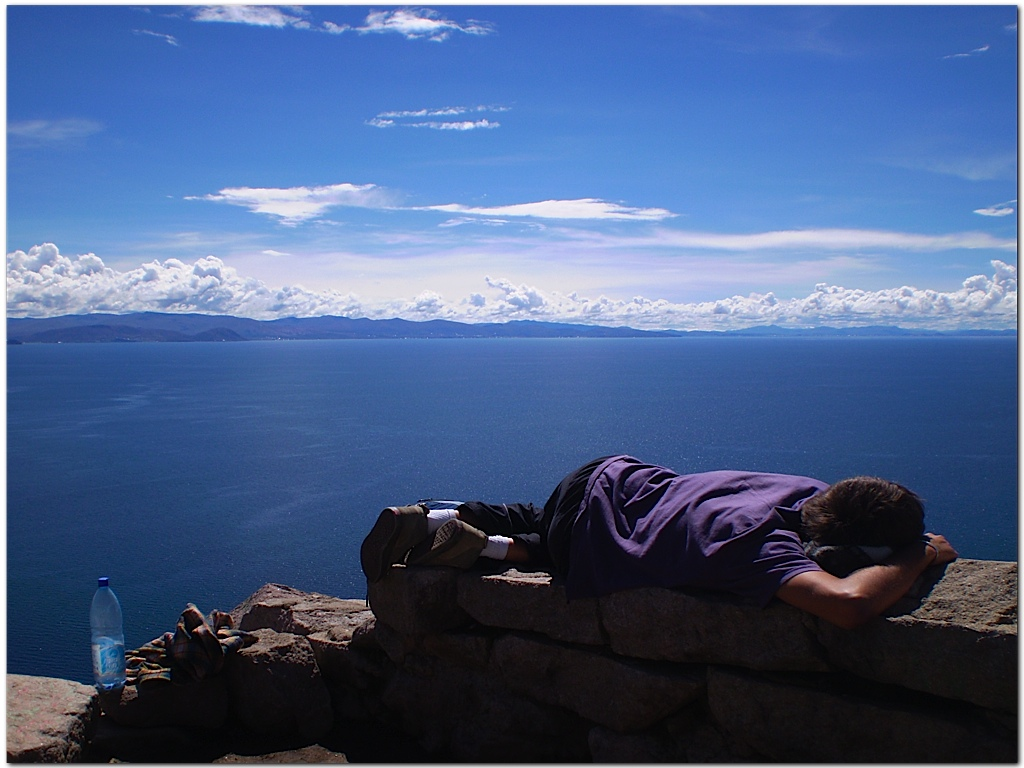
\includegraphics[width=300px]{images/P1160059.JPG} \textsc{\\Paz
en el lago.} \end{center}

Siempre que podemos desayunamos, almorzamos y cenamos en comedores municipales.
Son galpones llenos de mesitas (cada una correspondiente a cada cocinera), con
todos los precios iguales, informados en pizarrones colgados sobre la pared.
Viene más gente vaqueana del lugar que turismo, y nos encantan a pesar de la
nata de la leche.

Por Bolivia encontré común la imagen del Cristo completamente lastimado, luego
de los azotes. Es característico de este arte barroco-mestizo parece. Se le da
mucha bolilla al Cristo y la Virgen dolorosas, será por el pueblo oprimido
sobre el que instalaban esta Religión, tal vez. También vimos hoy muchas
ofrendas a la Pachamama. No me gustó que pedían todo material, pero nos
divertía ver la mezcla: tirando cerveza a la Madre Tierra, haciendo explotar
pirotecnia, con una cruz cristiana e incienso quemándose\ldots\ extraño, y un
toque milagrero. Pero vi otros devotos de la Pachamama que hablaban más,
digamos, a nuestro estilo (el de los chicos y yo): simple, y con amor y fe en el
centro.

¡Un beso enorme a todos!

Tute.

\subsection*{19 de Enero -- La Isla del Sol}

¡Hola, queridos! ¿Como andan? Este mail sale de
teclado norteamericano, en Perú. ¿Descuido o mucho turismo por
Cuzco?

Recorrimos Copacabana, la ciudad turística boliviana, lindante con el Lago
Titicaca. Divino. Comimos pescados más que pollos fritos por aquí, un placer.
Al otro día tomamos una lancha a la Isla del Sol.

La Isla del Sol es una islita montañosa de casi 20~km de largo por 8~km de
ancho. Se llega a su parte Norte luego de pagar \$15{\small BO}, y de unas dos o tres
horas de navegación. Es paradisíaca. Un nativo hizo de guía, llevándonos a
miradores y a las ruinas Incas que hay al Norte de la isla. Caminamos un buen
rato, y luego de unas charlas sobre su modo de vida e historia de la Isla, nos
describió el camino al Sur, donde descansaríamos y dormiríamos. Nos
despedimos, ya que él volvía a su pueblo, y nos sentamos un rato a descansar.

Como casi todos los días, en la mañana llovió, pero desde el mediodía
acompañó un buen sol. Desde este punto en que tomábamos mates se veían
varias playitas casi vírgenes, de arena clarita, agua azulada, y el lago y
otras islas cercanas. Quedábamos cinco viajeros, tres niños del lugar, y de
vez en cuando cruzaba algún pastor cuidando ovejas, no se porqué tan poquita
gente en tamaño lugar. Bajé a la playa para sentir el agua, daban ganas de
instalar una carpa y quedarse una semana de sereno ocio. El paisaje es perfecto,
las aves van y vienen, hay gran silencio interrumpido por ovejas, y rodean las
ruinas sobre la verde montaña. El agua es fresca, casi tan fría como la de
Mar del Plata; sólo molestan las algas del suelo. Huele un poco a mar, ya que
tiene muchos peces y es lago salado (se formó, como el Salar de Uyuni, a partir
un mar que cubría todo).

Subí fresco a donde me esperaban, y empezamos la caminata a la parte Sur. Cinco
horas de fuerte sol por la cresta de las montañas que dan forma, a la isla,
cansador pero perfecto. Cada ondulación significaba un increíble mirador al
Lago.

Ya en el Sur descansamos, leimos mirando el atardecer nublado y de vivos colores
celestes y rojos, cenamos bien, y a dormir, mucho. A las 5am nos levantamos para
ver si valía la pena salir a mirar el amanecer, pero estaba un poco nublado y
decidimos seguir durmiendo. El frío, ademas, es intenso cuando no hay sol.\\

Esa mañana (de ayer, 18) visitamos el Templo del Sol, casi en la punta sur de
la isla, y luego bajamos a una playita de rocas también casi virgen, donde nos
pasaría a buscar una lancha para volver a Copacabana (de película). A los 15
minutos apareció, subimos, y nos trajo de vuelta al pueblo, desde donde
empezaríamos el viaje a Perú.

Luego de trámites rápidos en la frontera, llegamos a la tarde a Puno, Perú.
Ahí visitamos a los Uros, una comunidad aborigen antigua distinta de los
Aymarás e Inkas. Ellos se instalaron literalmente en el Lago Titicaca, sobre
islas flotantes artificiales armadas a partir de la planta de Totora, para
escapar de los invasores Inkas. Ya dominaban la navegación con sus barcos de
Totora, uniéndolos y haciendo otros trabajitos formaban las mencionadas islas.
Las casas también son de Totora, los barcos, el suelo, todo; el paisaje es
sorpendentemente monocromático, de amarillos anaranjados. Por la humedad de su
hábitat sufren reuma desde los 30 años, si bien todos los días comen Totora
que tiene mucho calcio (y es rica).

Hay comunidades de Uros que prefieren no tener contacto con el turismo y
obviamente no las visitamos, pero éstos tenían todas las instalaciones y
estaban muy acostumbrados a recibirlos. Nos mostraban sus casas, sus
manualidades, nos contaban de su modo de organización (parte del dinero se
destina a un fondo común para ancianos enfermos, por ejemplo), de su escuela,
etc. Segun la estación del año mudan las islas, porque el nivel del lago
varía mucho y de no moverse se inutilizarían las estacas que las
inmovilizan. ``Imaginen --decía el guía-- que podrían aparecer en el lado
boliviano, ¡y eso es muy indeseable!'' Ahora gozan de paneles
solares, donación del ex presidente Fujimori. Se imaginan, ¡uno
se dormía con la vela encendida y se prendía fuego toda la comunidad! Cocinan
con fuego desde hace poquito, antes comían todo crudo.

Ahora hablan Aymará en las casas, mientras que la escuela y el turismo les
enseñan español. Los que conocimos son muy afectuosos.

Esa misma noche continuamos el viaje a Cuzco. Llegamos a la madrugada, nos
instalamos en un hostal, y salimos a caminar. El contraste con la vida boliviana
se nota mucho, realmente. Cuzco es una ciudad hermosísima, a la misma vez
preincaica, incaica y colonial. Sobre muros incaicos de enormes piedras de
granito perfectamente encastradas hay construidas grandes iglesias, y también
se conservan muros preincaicos (con piedras menos trabajadas y encastres menos
prolijos). Hay balcones de madera tipo galería en casi todas las casas,
trabajados minuciosamente.

En Bolivia nos hablaban con resentimiento de Perú, en Perú nos hablan a la
misma vez con humor y desprecio de Bolivia. Da un poco de tristeza.

Visitamos varios museos, y hoy sábado saldremos a unos bares. Mañana
caminaremos más tranquilos (no tantos museos), y pasado comenzamos el viaje a
Machu Picchu. Iremos por Ollantaytambó a Aguas Calientes, para volver luego por
la ruta alternativa: Santa María y Santa Teresita. Es la ruta más barata
que encontramos, tambien con ruinas durante el camino, y divertida de hacer
(colectivitos y caminatas). Hay otras rutas dignas de conocer: el Camino del
Inka largo, el corto, ir en bici, etc. Pero todo dolarizado, y no llegamos.
Encontramos al tren la menos entretenida de las opciones, dado que es rápido y
no hace paradas para conocer. El camino del Inca debe ser la mejor opción para
acercarse a Machu Picchu, pero no baja de U\$S 150 y de diez días de espera. Lo
podríamos hacer solos con agallas y con carpa, es que no trajimos lo segundo.

Un beso muy grande a todos;

Tute.


\section{Cuzco}

\subsection*{25 de Enero -- Cuzco y alrededores}

¡Hola, queridos! Muchas gracias por sus mails.

Una mañana empezamos el camino a Aguas Calientes. Dejamos las mochilas en el
hostal, y llevamos lo mínimo necesario sabiendo que esperaban 4 días de
movimiento. Empezamos por Pisaq, en un tour, donde caminamos un buen rato hasta
llegar a unas ruinas Inkas fenomenales. El trabajo faraónico que hacían sobre
las montañas para cultivar en forma de terrazas sorprende, aún más, que el
minucioso encastre de enormes piedras, que dan forma a todas las paredes (sean
templos, casas importantes, o las mismas terrazas).

El guía parecía muy culto, y no habló de nada ``místico'', todo
histórico-lógico. Muy interesante escucharlo. Por ejemplo, rompió mi amor con
la cruz andina, ``un invento más bien colonial'', a su decir. En realidad es
más moderna: se hizo famosa en una campaña política del 80'.

Luego visitamos Ollantaytambó, donde sorprenden las mismas cosas que en Pisaq.
Los esclavos subían enormes bloques de piedra a la montaña, y las lijaban con
agua y arena para que encastren perfectamente unas sobre otras (una macho y otra
hembra, además) de modo de lograr esas bellezas de fuertes construcciones.
Además, en la montaña de enfrente (donde choca el frío viento) almacenaban
toneladas de papas y carnes deshidratadas, una técnica que les permitía
almacenar alimentos por décadas.

A Pizarro y sus doscientos hombres se le hizo relativamente fácil la conquista,
dado que el 70\% de los miles de Inkas eran esclavos y no estaban satisfechos
con el Imperio. Además, el líder y su hermano estaban peleados, así que,
organizando esta oposición, pudo derrumbar el inmenso y entonces poderoso
imperio. Llamar ``Inkas'' a estos indios no es exacto: Inka significa en quechua
``hijo del sol'' y había sólo uno, el líder. El Sol es la deidad principal
Inka, de modo que su hijo era algo así como nuestro Mesías. Supongo que lo
correcto es llamar ``quechua'' a esta cultura.

Ahí tomamos un minibus al kilómetro 82 de esta ruta. Desde ahí
caminaríamos por las vías hasta Aguas Calientes, kilómetro 112
(recorreríamos 30~km), y de noche para que los guardias no nos lo impidieran.
¡``Turismo ciruja''! Además nos reconforta no tomar los
dolarizados trenes, crudo monopolio que cobra por un viaje de 40 minutos U\$S 8.
Y sí, en dólares, no les hablen de soles peruanos. La caminata de protesta me
costó numerosas y dolorosas ampollas, ya llegaré.

Llegamos al 82 al atardecer. Subimos a un café para hacer tiempo hasta las 4am,
nos atendió efusivamente un peruano que insistió tanto en servirnos, que
aceptamos tomar unos café con leche. Nos sugirió (la enorme sonrisa nunca se
le borró) que saliéramos después del último tren, a las 9pm, porque sino
llegaríamos a Aguas Calientes a la mañana y por ahí tendríamos que coimear
a algún guardia de allá que nos recibiera. Llegaríamos así de madrugada si
todo iba bien, antes del primer tren. Aceptamos esperar esas dos horas en su
nuevo restaurant, el primero en esta zona.

Nos mostró una galería donde nos dejó descansar, con vista a las escarpadas
montañas, al río, y a las vías donde pasaban eventuales trenes. Mirábamos
en silencio la desaparición del sol, pensando con ansiedad, emocionados, en
cómo sería lo que nos esperaba. Unos momentos con mucha magia.

Volvimos adentro para charlar un rato, y este hombre, Rubén, nos contó su
vida. Alrededor de 35 años, estudiante de chef, enfermero y administrador
hotelero; viajó por Bolivia, Chile y Argentina durante su formación, donde
recibió no pocos malos tratos, de los que aprendió a tratar a la gente como la
gente merece (o mejor). Hablaba de las grandes capitales como circos demasiado
artificiales, y de su charla se desprendía un inmenso amor por su madre tierra,
y por eso amaba poder ahora emprender este restaurant en este bellísimo punto
de su país. Sin embargo se le complica con la soledad, pero en la negociación
gana la serenidad de vida, la directa conexión con la naturaleza, las cercanas
ruinas indígenas que lo rodean, y la general alegría de los turistas que lo
visitan.

Nos despedimos agradecidos (a pesar de que los cafés costaban como nuestras
cenas), cenamos afuera unos sanguchitos, y estuvimos quince minutos vigilando a
los vigilantes, para saber cuándo lanzarnos a las vías. Una viejita nos vio
expectantes y nos sugirió, a las 9:40pm, empezar viaje: los guardias ya
estarían dormidos. ¡Con buena adrenalina empezamos viaje, a
saltar eufóricamente sobre los durmientes! Cuando las nubes no interrumpían la
luz de la luna llena, los picos nevados brillaban azulados. Me sentía tan
hermanado con la Naturaleza como nunca. Estábamos los chicos (Guido y Eugenio),
Laura (mochilera que iba a ir en tren, pero le tentó nuestra aventura), y yo.

A los 15 minutos encontramos las primeras ruinas, como Rubén nos indicó.
Entramos en medio de la oscuridad. De nuevo notamos la construcción hecha con
minuciosas piedras encastradas. Era movilizante estar solos en ese valle donde
antaño vivió una comunidad Inka, jóvenes turistas del siglo {\small
XXI}. Irónicamente, la realidad más concreta daba la sensación de estar
viviendo algo ficticio.

En el kilómetro 12 de nuestra caminata empezó a llover, ininterrumpidamente
hasta nuestra llegada. Como llevé zapatillas de Guido que me quedan grandes
(perdí las mías, que se desataron alguna vez de la mochila) las ampollas
fueron más violentas que las que siempre tuve, y realmente me molestaron para
llegar.

A la mitad del viaje ya llevaba un paso lento y cansado, a veces sufrido. Todos
estábamos igualmente exhaustos; como Eugenio lleva un paso rápido a veces se
sentaba a esperarnos, y lo encontrábamos dormido sobre alguna roca. Entre la
oscuridad y la lluvia asustaba el bulto, y nos costaba reconocerlo.

Luego de ocho horas de exigencia llegamos a Aguas Calientes, eran las 5:40am. El
primer hostal que se nos cruzó costaba 15 soles, Euge nos preguntó si estaba
bien y contestamos con una sentida risa. El precio no importaba dado el
cansancio, y además era bueno. A dormir mucho.

Nos despertamos a las 11am, desayunamos, y nos volvimos a dormir. Nos
despertamos de nuevo a las 3pm, Laura nos trajo almuerzo y comimos acostados.
Euge y Laura salieron a conocer, pero con Guido estuvimos durmiendo/leyendo
hasta las 7 de la tarde, hora en que nos levantamos obligadamente para comprar
las entradas a las ruinas de Machu Picchu. Cenamos unos sanguchitos de verduras,
y a volver a dormir. Un día de necesario y profundo descanso.

La siguiente mañana encaramos a las ruinas. Los chicos subieron a pie, yo en
los dolarizados colectivitos (malditas ampollas). Machu Picchu no sorprende por
el trabajo minucioso de sus construcciones, sólo los templos se muestran tan
trabajados, siendo todas las terrazas, casas y depósitos de piedras pequeñas
de cualquier forma, unidas por barro. Lo que sorprende de estas ruinas es que no
son sólo paredes o una unión de casitas, verdaderamente tiene forma de ciudad,
y los diversos puntos panorámicos permiten contemplarlo. La única emoción que
me provocó todo este día fue el primer vistazo, apenas cruzada la puerta de
entrada, cuando aparece de modo instantáneo frente a uno la eterna postal de
estas ruinas, pero la de verdad. Porque las ruinas anteriores, especialmente
Ollantaytambó, me recrearon muchos más pensamientos que esta ciudadela. Hice
el tour con guía del lugar, para entender todos los detalles que pudiera, y
realmente encontré pocas novedades frente a lo anterior. No pretendo
desmerecerlo, Machu Picchu es enorme y digno de conocerse, pero quiero mostrar
que se habla mucho de todo esto y sus precios son adecuados a su gran demanda,
mientras se menciona tan poquito del resto del territorio peruano, que atesora
varias y grandes ruinas indígenas. Es sin dudas un muy buen negocio, y una
visita interesantísima.

Bajamos a Aguas Calientes, y averig\"uamos para volver a Cuzco por el camino
alternativo (el barato). No hay otra opción (¡qué odio!) que
empezar el viaje tomando el tren a una represa hidroeléctrica: U\$S 8.
Caminamos otras dos horas por las vías para evitarlo (esta vez en ojotas), y
dormimos en un sucucho que había por ahí, a la vera de los rieles. Como los
chicos estaban muy cansados, bajé a pedir algo para cenar. Me había indicado
el dueño de este lugar una casita sobre las vías que corren más abajo.
Encontré ahí a una viejita y a su hijo cenando un buen plato de fideos. Les
pedí comida para tres, y acordamos en que unos sanguchitos con los fideos que
sobraban y con huevos fritos no estarían nada mal. Los llevé en una bolsa que
se condensaba, y eso comimos. ¡Riquísima cena!\\

La siguiente mañana tomamos colectivo a Santa María, y si bien nos íbamos a
quedar en sus aguas termales, no nos gustó, y tomamos un minibus directo a
Cuzco. Esto fue a las diez de la mañana de hoy.

El camino era increíble, con un agresivo precipicio y eventuales
desprendimientos de la montaña. Volvimos a sentir peligro. Cruzamos un Abra a
4000msnm, en ruta ya asfaltada pero con niebla, lluvia y varios derrumbes que
teníamos que atravesar. Los enormes paisajes dan a uno la sensación de
irremediable pequeñez.

A las 7 de la tarde llegamos duros de la incomodidad, luego de nueve horas en
una camionetita que andaba lento. Baño reparador, y a tomar cervezas por mi
querido Cuzco.

Al fin, Machu Picchu llegó como una consecuenca de todo lo que veníamos
haciendo. La ciudadela se cruzó justo después de nuestra recorrida por Bolivia
y de una buena caminata por las vías. El objetivo, nuevamente, fue el viaje, y
no el punto, digamos, final. Amo este viaje.

Ahora nos espera la bajada a Oruro y sus carnavales, conoceremos otros puntos
por el medio.

Un beso muy grande a todos. ¡Muchas gracias por su compañía, y
la info que mandaron!

Tute.

\section{Carnavales de Oruro} \subsection*{31 de Enero -- Sorata}

¡Hola queridos! ¿Cómo andan?

Aquí hace unos días empezamos a bajar. Hubiésemos esperado a la diablada
carnavalesca en Cuzco, pero la moneda peruana nos dejó casi sin billetes. El
cálculo del dinero que nos quedaba por día nos dejó boquiabiertos, decidimos
volver a Bolivia. Con paradas en Puno (Perú), y en Copacabana (Bolivia),
llegamos una mañana a Sorata para conocer, casi de casualidad ya que casi
nadie nos la nombró. Es la Capital del Trekking, y es una hermosura. Dicen que
al fondo está lleno de picos nevados, pero sólo podíamos ver las grandes
montañas verdes y cercanas, porque las nubes van y vienen, pero nunca se
separan del fondo.

La ciudad parece colonial, antigua; tiene hermosos edificios que alguna vez
fueron grandes casas, ahora abandonadas. Las paredes pintadas contrastan con los
ladrillos de construcción sin revoque que abundan por la Bolivia que conocimos.
(Al final no vamos a conocer la otra campana, la parte oriental; es el moño
para cerrar este viaje pero no llegamos.) Sin embargo, casi todas las
construcciones céntricas están ahora abandonadas.

Paramos en el hostal Mirador, a precio de Hostal, con vista de hotel de lujo.
Hicimos una caminata de tres horas (en cada curva, un buen punto panorámico) a
las Grutas de San Pedro, unas cuevas naturales cavadas en la montaña, de 400m
de largo. Tiene un lago que, según dicen, la profundidad máxima es de 400m
aprox. Al entrar encendieron las luces, y todos los murciélagos que iban de
acá para allá chillando se empezaron a calmar, únicos habitantes vertebrados
de las cuevas.

Unos chinos hace años bucearon por el lago, aparentemente encontraron que esta
cueva se comunica con otra a través del agua. Sin embargo nunca enviaron
detalles, y ya no vinieron investigadores extranjeros ni bolivianos a
comprobarlo. Raro.

El punto turístico parece mucho más organizado desde el Estado que muchos
otros que visitamos: entre el BID y otros fondos invirtieron casi U\$S 100.000
en folletos, construcciones, etc. Sin embargo, llegar es un poco difícil y el
turismo parece seguir siendo mochilero. Hay tres caminos desde Sorata: por la
ruta (debido a los derrumbes sólo la pudimos completar a pie), por una
montaña (debe ser divertido, gran desgaste físico), y por el río, imposible
en época de lluvias. La ruta hasta Sorata tampoco asegura la llegada, estas
montañas con clima tan húmedo se derrumban en forma constante.

El cuidador nos contó varios mitos de las cuevas, por los que
``mucha gente'' no se anima a investigarlas. Cómo gustan de los mitos;
¡las montañas se tragan personas porque son peligrosas, no
porque tienen vida y se enojan! Nos contaba también que antes había graffitis
en las rocas, los tuvieron que limpiar a todos. ``Son los peruanos, que vienen a
Bolivia a ensuciar.'' Igual que dos taxistas: ``ojo, chicos, que vienen muchos
peruanos a Bolivia para robar''. Me dan ganas de contestarles que es más
negocio robar en soles, pero más vale seguir con el tema del clima. Me enerva
pensar en el bruto prejuicio que estos comentarios empiezan a generar.

Volvimos de las cuevas bajo lluvia, esta vez con Euge usamos una hora y media.
Ahora se me está rompiendo una alpargata, voy a llegar de vuelta a casa
descalzo, parece. El placer de la vuelta será este viaje las zapatillas que me
esperan.

Y llegamos a La Paz. Paramos en el Hostal Carretero esta vez, más lejos y
barato, y con más onda social digamos. Tres españoles, dos andaluces de
Málaga y un gallego, hacían música y chistes, cuando no charlábamos entre
todos. El gallego hacía música desde botellas, cubiertos, el mueble de madera,
las camas de metal\ldots\ después contó que es profesor de teatro, la creativa
improvisación venía de algún lado. La pareja de Málaga, ya adultos,
parecían drogarse que daba miedo. Mientras fumaban cigarrillos nos contaban que
allá fuman mucho hachís (algo así como marihuana concentrada, explicaron),
que es muy buena porque viene de Marruecos. Marruecos, aprendí, es la meca de
los fumones. Anduvo Jimmy Hendrix entre otros, viendo elefantes rosas
sobrevolando 'Africa. Mucha droga cruza a Málaga en barco, por el Estrecho.
Cuando los helicópteros los están por descubrir, tiran los cargamentos al agua
(sellados de modo impermeable), y las lanchas se guarecen en el Estrecho de
Gibraltar, gobernado por ingleses, donde España no puede meter mano. ``Qué
buen negocio debe ser'', concluía el andaluz.

Por Bolivia vemos miles de mini-buses, muchos taxis, y pocas modernas
4$\times$4. Parece no haber clase media con Renault Clios o Ford Fiestas.

¡Ya es 31! Pasado mañana vamos a los Carnavales, nos advierten
de ladrones y precios dolarizados. De ahí tomaremos tren a Villazón si
conseguimos, y colectivo de La Quiaca a Rosario.

Un beso muy grande a todos. ¡Gracias por su compañía!

Tute.

\subsection*{4 de Febrero -- Carnavales de Oruro}

¡Hola, queridos! ¿Cómo andan?

Nosotros muy bien: viajamos el primero de Febrero a Oruro, y llegamos de noche.
El alojamiento está muy caro en temporada tan alta, así que dormimos en un
proyecto de hostel, sobre el piso de cemento de la construcción. A \$20{\small
BO} bolivianos, ¡como un hostal bueno de otras ciudades! Sin ducha, sólo un
limpio inodoro y el sucio suelo. Entonces había alternativas baratas, sólo hay
que llegar, y caminar buscando.

Esa noche previa al carnaval, salimos a caminar por la calle principal, toda
rodeada de gradas, algunas pobladas con bandas tocando música carnavalesca.
Tomamos unos Singani, aguardiente de Bolivia, mezclados con té o leche
calientes, muy rico. Y caminamos un buen rato, nos hicimos amigos de un montón
de gente. El circo que se arma es grande. Esa noche parecía que todos los
orurenses habían salido a caminar y a bienvenir turistas. Sólo Euge se cruzó con
uno medio cruzado, lo trataba con tenso desprecio, al principio al menos. Varios
nos dijeron que en Argentina los discriminamos y los tratamos de ``bolitas'', a
todos les contestamos que sin dudas es verdad, de hecho lo sienten, pero que
también hay gente más lógica, como en todos lados incluyendo Bolivia. Casi todos
lo entienden, pero algunos generalizan.

Nos acostamos a las 5am, horas antes de que empiece el carnaval. La bebida
desconocida nos mató: tirados en el suelo sentíamos que las peladas paredes
daban vueltas sobre nosotros. Queríamos ``tirar el ancla'' (bajar un pie de la
cama para que se inmovilice el mundo) pero más abajo que el piso no podíamos
llegar, ¡qué desesperación! Una tortura, hasta que nos dormimos.

Nos despertamos tarde (tipo 11, empezados los bailes), compramos pasaje en
colectivo a Potosí (directo a Villazón no había), y empezamos a caminar por la
calle principal para mirar los grupos musicales y de bailarines. Cada grupo
consta de unas 40 mujeres y unos 40 hombres, todos con unos trajes
increíblemente trabajados y coloridos, bailando alegremente al compás de las
bandas, que se forman de unos 30 músicos, entre trombones, trompetas, tambores,
redoblantes, etc. Juro que no exagero: ¡cada grupo, de los cientos que hay, se
conforma de más de 100 artistas! El camino que recorren bailando tiene más de
3~km, imaginen que empezaron a las 7am, y terminaron a las 5am del día
siguiente: 22 horas de grupos, y uno no se cansa de mirarlos.

Caminar por las calles es complicado: donde no hay gradas hay cientos y cientos
de personas yendo y viniendo, tirándose espuma y globos de agua, y muriéndose de
risa. ¡El circo que se arma es enorme! Subimos hasta la plaza, donde los grupos
dan una vuelta para seguir subiendo a la montaña. Aquí se concentra mucho el
turismo, las gradas cuestan más de 100 bolivianos, más de 14 dólares. Para los
mochileros acostumbrados a precios de Bolivia es impensable. Así que miramos
desde las libres esquinas. Aquí los bailarines se ponían eufóricos y los
espectadores también, era espectacular. Los primeros bailaban como locos, ¡como
si fuera carnaval!, y los segundos alentaban de un modo que ponía la piel de
gallina. Mucha fuerza. Los globitos de agua cruzaban la calle, iban de grada en
grada. Todas risas. De los miles de personas que vimos, sólo vimos dos enojadas
por lo mojado. ¡Que se jodan! La gente los cargaba siguiendo la diversión.

Seguimos subiendo hasta la Iglesia de la Virgen de la Candelaria, donde el
camino se ensancha en forma de campo dejando lugar a los grupos para mostrar su
arte. Encontramos unos asientos en primera fila a 15 bolivianos, nos sentamos
sin dudarlo. Aquí se reunían los familiares de los artistas, casi todos
bolivianos y estos tres turistas. Llegaban los grupos, se abrían para avanzar
bailando, la banda caminaba llenando el abierto ambiente con su música, y, luego
de un rato, los artistas entraban en la gran iglesia. El espectáculo de gente es
tan numeroso, tan inmenso, y las bandas hacen una música tan fuerte y alegre,
que verdaderamente emociona. Las montañas se veían llenas de gente, como en los
rallys. ¡Los globos cayendo desde arriba daban miedo!

Los grupos llegan de este modo artístico a orar a la Virgen de la Candelaria,
agradeciendo unas cosas y pidiendo por otras. Además de mucha historia y
cultura, acá el carnaval tiene matices religiosos. ¡Igual que en Pergamino!

Los bailarines tienen cascabeles en las botas, parte de la música es creada por
sus bailes. Los grupos que más me impresionaron fueron las diabladas: un
conjunto de diablos vestidos con los trajes más espectaculares y enormes,
bailando como locos, seguidos por un arcángel, que guía con sus Virtudes a otro
grupo de diablos, los Pecados Capitales. Esto del arcángel empezó este 2008
parece. Estos grupos jugaban con fuegos de artificio, y con una música de lo más
movida, además de ser los más numerosos. Impresionaba. También provocaban gran
emoción las Morenadas, sobre los negros traidos a trabajar a Potosí. Todas las
máscaras son, sin excepción, dignas de admiración.

Nos acostamos tipo 4am, antes de que terminara todo porque moríamos del sueño.
Bajamos al proyecto de hostal, y dormimos hasta las 9. Desayunamos charqui
(carne de llama disecada), y estos días comimos también ishbi (tipo cornalitos,
pero empanados y del Titikaka), anticuchos (carne, riñones o corazón; asados con
un aderezo lujurioso y a la vez barato), y ceviche (pejerrey --en nuestro caso--
cocinado con limón y otros aderezos, pero sin calor; crudo para nuestras
costumbres, se puede decir). Todo en sucuchos en la calle, todo de lo más rico y
sabroso.

Tomamos el cole a Potosí, y dado que no salían de ahí coles a Villazón (Bolivia
en carnaval se detiene, y todos festejan) tomamos una Toyota junto con otros 6
pasajeros bolivianos. ¡Eramos diez en la Land Cruiser, en un viaje de 8 horas!
La pasamos bien a pesar de que el traste sigue cuadrado. Ya bajando a Argentina
empezamos a recordar anécdotas del viaje, nuestros compañeros escuchaban
divertidos. En un momento nos callamos: empezamos a escuchar noticias argentinas
en tonada argentina: {\small AM}630. Dijo el conductor: ``¿Saben para qué la
puse? ¡Para que escuchen! ¡Y se callen un rato!'', y risas de todo el auto,
había muy buena onda. Pinchamos nada menos que tres cubiertas en el camino; en
la última, ya secos de repuestos y mientras peleaban con parches improvisados,
subimos a un cole que justo pasaba y amablemente aceptó a los nueve pasajeros.
El pobre conductor de la camioneta se quedó a esperar no sé qué cosa. Cambiar
las ruedas con ese frío era un sufrimiento.

Llegamos a la frontera de madrugada. Cruzamos hoy a La Quiaca, ¡bienvenidos a
Argentina! Tenía ganas, ya. El Pasaporte está quedando hermoso con tantos
sellos. Comimos medialunas, facturas, bizcochos; no lo podemos creer porque
podríamos haber comprado también pan ``felipe'', el ``pan de verdad''. En fin,
¡comemos todo lo que extrañamos, y vamos a extrañar todo lo que comimos!

En un rato sale el cole, mañana 5 de Febrero llegamos al mediodía a Rosario.
Seguro caeré en la tarde por Perga. Estamos felices, luego de semejante viaje.

¡Disfruten de por lo menos 5 meses sin noticias viajeras! 11 meses, a juzgar por
las deudas contraídas estos días.

Un abrazo muy grande a todos, y muchas gracias por su compañía. Nos vemos;

Tute.



\backmatter
\chapter{Agradecimientos}
\begin{flushright}
\item \emph{\small ``El agradecimiento en la mayor\'ia de los hombres no es
sino un oculto deseo\\de recibir mayores beneficios.''\\
Fran\c{c}ois de La Rochefoucauld}
\end{flushright}

No fue f\'acil dedicar el libro. \textexclamdown Las concisas l\'ineas que
pretend\'ia se inundaron de nombres y motivos! A la minuciosa revisi\'on
sobrevivi\'o el (ciertamente sentido) clich\'e: quedaron los viejos, y mis
amigos y compa\~neros de viajes Ezequiel, Guido y Eugenio. Ser\'a que no
merecieron cap\'itulo aparte pero, sea como sea, sigue la lista de las
personas a quienes quiero agradecer en forma especial:

\begin{itemize}
  \item A Julio Godoy, quien me llev\'o de la oreja a cruzar la Cordillera en
  bici a mis 14 a\~nos, con su auto de apoyo conducido por mi t\'io, otro
  viajero de profesi\'on. Fue el primer \emph{viaje}, y no lo pude creer.
  \item A la familia espa\~nola, especialmente a ``Eugen\'in'', quien se
  tom\'o vacaciones en las semanas que los visitar\'ia para ense\~narme buena
  parte de Espa\~na y Asturias.
  \item A los Piaggio, especialmente a Gustavo e Ina. Mi casa y Hogar en
  Alemania.
  \item A Axel Becker, otro viajero de profesi\'on (pero este de verdad).
  Luego de dejarme su bicicleta para conocer los alrededores de G\"ottingen,
  con generosidad y sonrisa me la dej\'o para todo el viaje por el sur
  alem\'an tambi\'en.
  \item A Mangacha y a Richard, quienes me ofrecieron un hogar mucho m'as
  cercano que Am'erica, en caso de que no me encontrara a gusto en Alemania.
  \item A Claus. No se preocup\'o de integrarme a una charla de alemanes, sino
  para ofrecerse de gu\'ia y mostrarme lugares imperdibles para la bici. Estas
  actitudes, dignas de imitaci\'on, dan belleza al mundo.
  \item A Sim\'on y Ale Drucaroff. Sin su incentivo y ayuda dif\'icilmente
  hubiera llegado a armar Relatos de Viajes a partir de aquella desordenada
  seguidilla de e-mails.
\end{itemize}

En fin, agradezco a quienes se relacionan como Humanos. Por esa obvia pero a
veces olvidada simpleza, uno vive tan plenamente como s\'olo un Humano puede,
y merece, hacerlo.

\newpage
\thispagestyle{empty}

\chapter{Ep\'ilogo}
\begin{flushright}
\item \emph{\small ``Lo mejor de los viajes es lo de antes y lo de
despu\'es.''\\
Maurice Maeterlinck}
\end{flushright}

Me parece casi necesario viajar, seguramente, porque en cada viaje crec\'i un
poquito, evolucion\'e como persona, pens\'e cosas que nunca --en la vida
diaria-- pienso. Vuelvo cuestionando cosas, celebrando otras, con ganas de
empezar algo nuevo y de dejar algo viejo; en fin, con ganas de mejorar.

Encontr\'e que en la vida curricular no cuento con la simpleza y apertura
mental que tengo de viaje, lo atribuyo a dos cosas.

La primera es que estar de viaje implica un corte en mi rutina, dejando todo
el tiempo libre para ocupar el cerebro en lo que quiera, sin obligaciones
pendientes. Estoy abierto a pensamientos que en la rutina juzgar\'ia como
``p\'erdidas de tiempo'', y que sin embargo son m\'as profundos y de largo
plazo que los que tengo durante el a\~no.

La segunda raz\'on es que los tiempos de fin de a\~no (que es cuando
generalmente tengo vacaciones) se prestan para estas evaluaciones: qu\'e se
logr\'o en el a\~no pasado, cu\'anto se lo disfrut\'o, qu\'e ser\'ia bueno
hacer (o dejar de hacer) en el a\~no entrante. Es m\'as f\'acil de que surjan
esos pensamientos en estas \'epocas del a\~no, mirar si el camino recorrido se
acerca a lo que queremos y creemos bueno, o hay que ajustarlo un poco.

En cambio, ocuparme de estos cuestionamientos ``de fondo'' durante el a\~no,
me alejan de las metas m\'as cortitas y cercanas (aprobar el examen que se
acerca, terminar el trabajo a tiempo). M\'as vale terminar las tareas que
estoy haciendo, y, una vez concluidas, hacer un entretiempo para evaluarlas.
As\'i, creo, me acerco a un equilibrio, y voy proponiendo peque\~nas y grandes
metas a mi vida, e intento seguirlas.

\textexclamdown Pensar que en un principio cre\'ia que viajar se trataba de
divertirse y de mejorar mi entrenamiento en bici! La verdad es que la
experiencia result\'o siempre mucho m\'as espiritual.

Por eso me parece tan importante salir a conocer lugares. Descubro ahora que,
en gran medida, por eso amo viajar.\\

Eugenio Costa.

26 de Diciembre de 2007

\end{document}
